

\documentclass[10pt]{article}
% \documentclass[10.8pt, a4paper, USenglish, twocolumn]{article}

\usepackage{isaks_template} % Contains all included packages. See isaks_template.sty.

% latex margins
% \linespread{1.5}
% \newgeometry{vmargin={15mm}, hmargin={25mm,37mm}}
\newgeometry{vmargin={15mm}, hmargin={30mm,30mm}}
%
% \title{Project Thesis\\ Solving the Biharmonic Equation using \\ a Continuous Interior Penalty Method}
% \author{Isak Hammer, \\[1cm]{\small Advisor: André Massing} }

\begin{document}


\begin{titlepage}
    \begin{center}
        \vspace*{1cm}

        \Huge
        \textbf{Master Thesis}

        \vspace{0.5cm}
        \Large
        Solving Cahn-Hilliard equation using a CutCIP method   \\

        \vspace{1.5cm}

        \textbf{Isak Hammer} \\
        \vspace{0.5cm}
        Supervisor: André Massing \\
        \vspace{0.5cm}
        \today


        \vfill

        \vspace{0.8cm}

        % \includegraphics[width=0.5\textwidth]{figures/front_page/molly.jpeg}\\

        \Large
        Department of Mathematical Sciences\\
        Norwegian University of Science and Technology\\

    \end{center}

\end{titlepage}
    % \begin{titlepage}
    %     \maketitle
    %     \begin{figure}
    %     \centering
    %     % \includegraphics[width=0.5\textwidth]{figures/front_page/dog.jpg}\\
    %     \includegraphics[width=0.5\textwidth]{figures/front_page/molly.jpeg}\\
    %     \end{figure}
    %     \thispagestyle{empty}
    % \end{titlepage}


    \newpage




    \section{Introduction}


\begin{frame}{Introducing Myself}
    \begin{columns}
        % Column 1
        \begin{column}{0.5\textwidth}
            \begin{itemize}
                \item Isak Hammer, 27 year old, Lofoten
                \item Graduate student in Industrial Mathematics
                \item Research Focus: Numerical methods for Partial Differential Equations (PDEs).
            \end{itemize}
        \end{column}

        % Column 2
        \begin{column}{0.5\textwidth}
            \begin{figure}
                \centering
                \includegraphics[width=0.7\textwidth]{figures/isak.jpg}
            \end{figure}
        \end{column}
    \end{columns}
\end{frame}

\begin{frame}{Importance and Motivation of the Cahn Hilliard Equation}
    \begin{columns}
        % Column 1
        \begin{column}{0.5\textwidth}
            \begin{itemize}
                \item Thermodynamically modelling of a two-component liquid separation\footnotemark[1].
            \item Modelling of so-called lipid rafts in biological membrane dynamics \footnotemark[2].
            \end{itemize}
        \end{column}
        \begin{column}{0.5\textwidth}
            \begin{itemize}
                \item Droplet dynamics, i.e., coalescence, breakup and movement by coupling with Navier-Stokes \footnotemark[3].
            \end{itemize}
        \end{column}
    \end{columns}
    \footnotetext[1]{\fullcite{cahn1959free}}
    \footnotetext[2]{\fullcite{yushutin2019computational}}
    \footnotetext[3]{\fullcite{zimmermann2019calculation}}
\end{frame}

\begin{frame}
    \begin{block}{The Cahn Hilliard Equation}
        The general Cahn Hilliard Equation  has the form $u( x, t): \Omega \times [0,T] \mapsto [-1,1]   $ s.t.
            \[
            \begin{split}
                 u_t+\Delta\left(\varepsilon \Delta u-\frac{1}{\varepsilon} f(u)\right)&=0 \quad \text{in } \Omega \\
\partial_n u=\partial_n \Delta u& =0 \quad \text{on } \Gamma  \\
 u & =u_0 \quad \text{on } \Omega
            \end{split}
            \]
where $f(s)=F^{\prime}(s)$ and $F(s)=\frac{1}{4}\left(s^2-1\right)^2$ and $\Omega \subset \mathbf{R}^d, d=2,3$, is a bounded domain.
\end{block}

\begin{block}{Challenges}
    \begin{enumerate}
        \item Highly nonlinear and stiff. Often practical applications require $\varepsilon \ll 1$.
        \item 4th order system.
        % \item Conservation of mass and the Neumann conditions conditions.
    \end{enumerate}
\end{block}

\end{frame}

\begin{frame}
    \begin{block}{Why Finite Element Method (FEM)}
        \begin{enumerate}
            \item \textbf{Robust mathematical framework}
            \item \textbf{Can easily handle complex geometries}
            \item \textbf{High flexibility of basis functions}
            \item \textbf{Other: } Supports adaptive refinements, easily adaptable to multi-physics problems ++ .
        \end{enumerate}
    \end{block}
\end{frame}

% \begin{frame}
%     \begin{block}{Strategy to solve the Cahn-Hilliard problem on smooth domains}
%         \begin{enumerate}
%             \item Solve the biharmonic problem $\Delta ^2 u = f$ for polygonal domains.
%             \item Modify the method to handle smooth domains.
%             \item Utilize the time integration to handle non-linearity.
%         \end{enumerate}
%     \end{block}
% \end{frame}

% \begin{frame}
%     \begin{block}{Strategy to solve the Cahn-Hilliard problem on smooth domains}
%         \begin{enumerate}
%             \item First find a suitable method to solve an 4th order PDE for polygonal domains.
%             \item Modify the problem formulation to take account for smooth domains.
%             \item Utilize the time integration to handle nonlinearity.
% \item \textcolor{red}{Make the time-steps small enough or implement adaptivity time schemes.}
%         \end{enumerate}
%     \end{block}
% \end{frame}


% \begin{frame}
% \begin{columns}
% \column{0.55\textwidth}
% \begin{block}{The Biharmonic Problem}
% Let $\Omega \subseteq \mathbb{R} ^d$ be a bounded domain with boundary $\Gamma $ . Let the biharmonic problem have the form s.t. $u:\Omega \mapsto \mathbb{R} $,
% \begin{equation}
% \label{eq:bi_problem}
% \begin{split}
% \Delta^2 u + \alpha u & = f( x) \quad \text{in } \Omega, \\
% \partial_{n} u & = g_{1} \quad \text{on } \Gamma , \\
% \partial_{n} \Delta u & = g_{2} \quad \text{on } \Gamma . \\
% \end{split}
% \end{equation}
% Here is $\Delta ^2 = \Delta \left( \Delta \right) $ the biharmonic operator. The functions $g_{1},g_{2}: \Omega \to \mathbb{R}$ are denoted as boundary conditions.
% \end{block}

% \column{0.45\textwidth}
% \begin{figure}[htpb!]
%     \centering
%     \begin{tikzpicture}
%         % Circle
%         \draw (0.0,0.0) circle (1.5cm);
%         \fill[blue!30] (0.0,0.0) circle (1.5cm);

%         \draw[->, line width=1.0pt] ({1.5*cos(65)}, { 1.5*sin(65) }) -- ({ 2.5*cos(65)  }, { 2.5*sin(65)  }) node[ above left] {$n $};
%         % \draw[->, line width=1.0pt] ({1.5*cos(45)}, { 1.5*sin(45) }) -- ({ 1.5*cos(45) - 1.5*sin(45) }, { 1.5*sin(45) + 1.5*cos(45) }) node[ above right] {$t $};

%         % Labels
%         \node[below right] at (0.5,0.5) {$\Omega$};
%         \node[below right] at (-1.5,-1.2) {$\Gamma$};
%     \end{tikzpicture}
%     \caption{ Illustration of the domain $\Omega $, the boundary $\Gamma $ and the normal vector $n$. }
%     \label{fig:domain_construction}
% \end{figure}
% \end{columns}

% \end{frame}

\begin{frame}
    \frametitle{The Biharmonic Problem (on a polygon)}
    \begin{columns}
        \column{0.55\textwidth}
        \begin{block}{}
            Let $\Omega \approx \Omega_{h} = \mathcal{T}_{h}$ be a bounded \textcolor{red}{polygonal} domain with boundary $\Gamma $ . Let the biharmonic problem have the form s.t. $u:\Omega \mapsto \mathbb{R} $,
            \begin{equation}
                \label{eq:bi_problem}
                \begin{split}
                    \Delta^2 u + \alpha u & = f( x) \quad \text{in } \Omega, \\
                    \partial_{n} u & = 0 \quad \text{on } \Gamma , \\
                    \partial_{n} \Delta u & = 0 \quad \text{on } \Gamma . \\
                \end{split}
            \end{equation}
            Here is $\Delta ^2 = \Delta \left( \Delta \right) $ the biharmonic operator.
        \end{block}

        \column{0.45\textwidth}
        \begin{figure}[htpb!]
            \centering
            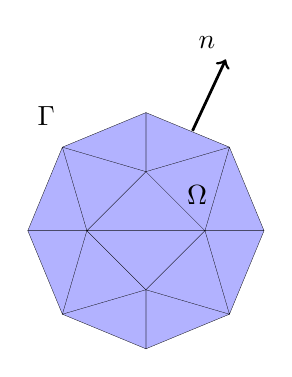
\begin{tikzpicture}
                % FIGURE OF FITTED MESH
                % Boundary points
                \foreach \i in {0, 45, ..., 315} {
                    \coordinate (boundary-\i) at (\i:1.5cm);
                }
                % Interior points
                \coordinate (interior-1) at (0.75, 0);
                \coordinate (interior-2) at (-0.75, 0);
                \coordinate (interior-3) at (0, 0.75);
                \coordinate (interior-4) at (0, -0.75);

                % Create a cycle connecting all the boundary points
                \fill[blue!30] (boundary-0) -- (boundary-45) -- (boundary-90) -- (boundary-135) -- (boundary-180) -- (boundary-225) -- (boundary-270) -- (boundary-315) -- cycle;

                % Labels
                \node[below right] at (0.4,0.7) {$\Omega $};
                \node[below right] at (-1.5,1.7) {$\Gamma $};

                % Triangulation (manually specified)
                \draw[line width=0.1pt] (boundary-0) -- (boundary-45) -- (interior-1) -- cycle;
                \draw[line width=0.1pt] (boundary-45) -- (boundary-90) -- (interior-3) -- cycle;
                \draw[line width=0.1pt] (boundary-90) -- (boundary-135) -- (interior-3) -- cycle;
                \draw[line width=0.1pt] (boundary-135) -- (boundary-180) -- (interior-2) -- cycle;
                \draw[line width=0.1pt] (boundary-180) -- (boundary-225) -- (interior-2) -- cycle;
                \draw[line width=0.1pt] (boundary-225) -- (boundary-270) -- (interior-4) -- cycle;
                \draw[line width=0.1pt] (boundary-270) -- (boundary-315) -- (interior-4) -- cycle;
                \draw[line width=0.1pt] (boundary-315) -- (boundary-0) -- (interior-1) -- cycle;

                % Triangulation between interior points
                \draw[line width=0.1pt] (interior-1) -- (interior-2) -- (interior-3) -- cycle;
                \draw[line width=0.1pt] (interior-1) -- (interior-2) -- (interior-4) -- cycle;

                \draw[->, line width=1.0pt] ({1.4*cos(65)}, { 1.4*sin(65) }) -- ({ 2.4*cos(65)  }, { 2.4*sin(65)  }) node[ above left] {$n $};

            \end{tikzpicture}
            \caption{ Illustration of the mesh $\Omega_{h} $, the boundary $\Gamma $ and the normal vector $n$. }
            \label{fig:domain_construction}
        \end{figure}
    \end{columns}
\end{frame}



\begin{frame}
\frametitle{ $C^0$ Interior Penalty Method (CIP) for the Biharmonic Problem }

\begin{block}{}
The proposed numerical scheme is to find an  $w \in V_{h}$ .t.
\begin{equation*}
\label{eq:CP_A_F}
a_{h}( w, v )   = l_{h}( v) = ( f,v)_{\Omega } , \quad \forall v \in V_{h}  .
\end{equation*}
where
\begin{equation*}
\begin{split}
a_{h} \left( w, v \right)   =&
    \left( \alpha  w, v \right) _{\Omega }   +  \left( \Delta  w, \Delta v \right) _{\Omega } \\
 & +
  \left( \mean{  \Delta  w }, \jump{ \partial _{n }v} \right)_{\mathcal{F}_{h}}  +
 \left( \mean{ \Delta  v }, \jump{ \partial _{n}w }      \right)_{\mathcal{F}_{h}}  + \frac{\gamma }{h}  \left( \jump{ \partial _{n} w}, \jump{ \partial _{n} v   }   \right)_{\mathcal{F}_{h}}
 % l_{h}( v_{h}) & =  \left( f, v \right) _{\Omega }
\end{split}
\end{equation*}

Which is inspired from Brenner2012 \footnotemark[1]
\end{block}

\footnotetext[1]{\fullcite{brenner2012}}

\end{frame}


\begin{frame}
\frametitle{Cut Finite Element Method (CutFEM)}

\begin{block}{Unfitted mesh vs fitted mesh}
    CutFEM is a numerical method for solving partial differential equations (PDEs) using an unfitted mesh.

\begin{figure}
    \centering
    % First TikZ picture
    \begin{minipage}{0.45\textwidth}
        \centering
        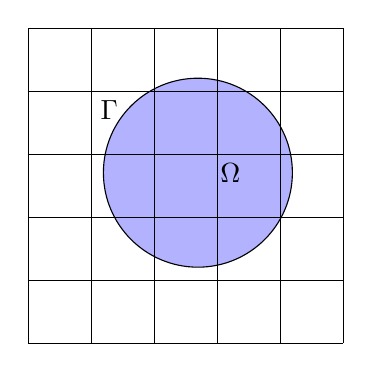
\begin{tikzpicture}[scale=0.80]
            \draw[fill=blue!30] (0.2, 0.2) circle (1.5cm);
            % Background mesh
            \foreach \i in {-2.5, -1.5, ..., 2.5} {
                \draw[line width=0.1pt, shift={(-2.5,\i)}] (0,0) -- (5,0);
                \draw[line width=0.1pt, shift={(\i,-2.5)}] (0,0) -- (0,5);
            }
            % Labels
            \node[below right] at (0.4,0.5) {$\Omega $};
            \node[below right] at (-1.5,1.5) {$\Gamma $};
            % \draw[blue, thick] (-2.5, -2.5) rectangle (2.5, 2.5);
        \end{tikzpicture}
    \end{minipage}
    \hfill
    % Second TikZ picture
    \begin{minipage}{0.45\textwidth}
        \centering
        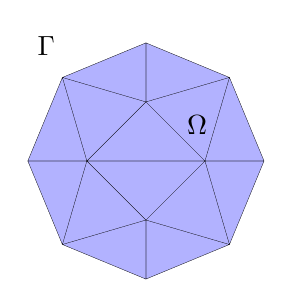
\begin{tikzpicture}[scale=1.0]
            % FIGURE OF UNFITTED MESH
            % Boundary points
            \foreach \i in {0, 45, ..., 315} {
                \coordinate (boundary-\i) at (\i:1.5cm);
            }
            % Interior points
            \coordinate (interior-1) at (0.75, 0);
            \coordinate (interior-2) at (-0.75, 0);
            \coordinate (interior-3) at (0, 0.75);
            \coordinate (interior-4) at (0, -0.75);

            % Create a cycle connecting all the boundary points
            \fill[blue!30] (boundary-0) -- (boundary-45) -- (boundary-90) -- (boundary-135) -- (boundary-180) -- (boundary-225) -- (boundary-270) -- (boundary-315) -- cycle;

            % Labels
            \node[below right] at (0.4,0.7) {$\Omega $};
            \node[below right] at (-1.5,1.7) {$\Gamma $};

            % Triangulation (manually specified)
            \draw[line width=0.1pt] (boundary-0) -- (boundary-45) -- (interior-1) -- cycle;
            \draw[line width=0.1pt] (boundary-45) -- (boundary-90) -- (interior-3) -- cycle;
            \draw[line width=0.1pt] (boundary-90) -- (boundary-135) -- (interior-3) -- cycle;
            \draw[line width=0.1pt] (boundary-135) -- (boundary-180) -- (interior-2) -- cycle;
            \draw[line width=0.1pt] (boundary-180) -- (boundary-225) -- (interior-2) -- cycle;
            \draw[line width=0.1pt] (boundary-225) -- (boundary-270) -- (interior-4) -- cycle;
            \draw[line width=0.1pt] (boundary-270) -- (boundary-315) -- (interior-4) -- cycle;
            \draw[line width=0.1pt] (boundary-315) -- (boundary-0) -- (interior-1) -- cycle;

            % Triangulation between interior points
            \draw[line width=0.1pt] (interior-1) -- (interior-2) -- (interior-3) -- cycle;
            \draw[line width=0.1pt] (interior-1) -- (interior-2) -- (interior-4) -- cycle;

            % \draw[blue, thick] (-2.5, -2.5) rectangle (2.5, 2.5);

        \end{tikzpicture}
    \end{minipage}


    % \caption{Mesh comparison: unfitted mesh (left) adheres to domain and boundary, while fitted mesh (right) employs a triangular mesh for polygonal approximation of the circular domain.}
    \label{fig:domain_mesh}
    \end{figure}
\end{block}

\end{frame}

\begin{frame}
    \frametitle{Cut Finite Element Method}
Background Mesh
    \begin{block}{}
        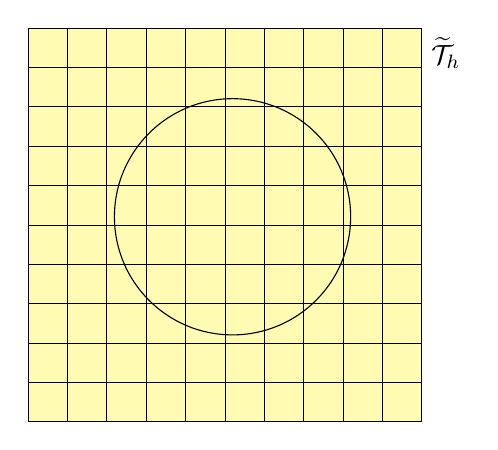
\begin{tikzpicture}[scale=1.0]

            \fill[yellow!30] (-2.5,2.5) -- (2.5,2.5) -- (2.5,-2.5) -- (-2.5,-2.5) -- cycle;

            \draw (0.1, 0.1) circle (1.5cm);
            % Background mesh
            \foreach \i in {-2.5, -2, ..., 2.5} {
                \draw[line width=0.1pt, shift={(-2.5,\i)}] (0,0) -- (5,0);
                \draw[line width=0.1pt, shift={(\i,-2.5)}] (0,0) -- (0,5);
            }


            % Labels
            \node[below right] at (2.5,2.5) {$\widetilde{\mathcal{T}}_{h}$};
        \end{tikzpicture}
    \end{block}
\end{frame}

\begin{frame}
    \frametitle{Cut Finite Element Method}
    Active Mesh
    \begin{block}{}
        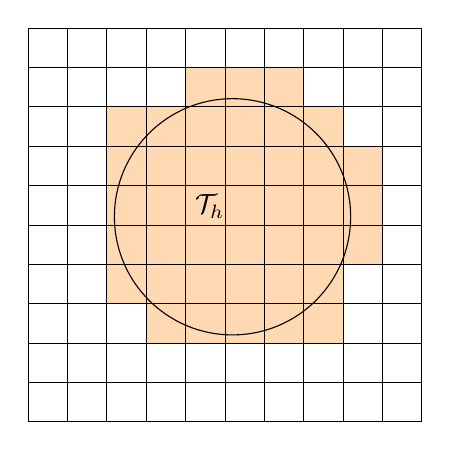
\begin{tikzpicture}[scale=1.0]

            % POTENTIAL ACTIVE MESH
            \fill[orange!30] (2,2) -- (2,-1.5) --(-1.5,-1.5) -- (-1.5,2) -- cycle;

            % ELEMENTS WITH NO INTERSECTION
            % lower left
            \fill[white] (-1.5,-1.5) rectangle (-1.0,-1.0);
            \fill[white] (-1.5,2.0) rectangle (-1.0,1.5);
            \fill[white] (-1.0,2.0) rectangle (-0.5,1.5);
            \fill[white] (2,2) rectangle (1.5,1.5);
            \fill[white] (1.5,2) rectangle (1.0,1.5);
            \fill[white] (2,1.5) rectangle (1.5,1.0);
            \fill[white] (1.5,-1) rectangle (2,-1.5);
            \fill[white] (1.5,-0.5) rectangle (2,-1.0);

            % CUT ELEMENTS
            \fill[orange!30] (-0.5,2.0) rectangle (1.0,1.5);
            \fill[orange!30] (-1.5,1.5) rectangle (0.0,1.0);
            \fill[orange!30] (0.5,1.5) rectangle (1.5,1.0);
            \fill[orange!30] (-1.5,1.0) rectangle (-1.0,-1.0);
            \fill[orange!30] (-1.0,-0.5) rectangle (-0.5,-1.5);
            \fill[orange!30] (-0.5,-1.5) rectangle (1.5,-1.0);
            \fill[orange!30] (1.5,-1) rectangle (1.0,-0.0);
            \fill[orange!30] (1.5,-0.5) rectangle (2.0,1.0);
            \fill[orange!30] (1.0,0.5) rectangle (1.5,1.0);

            \draw (0.1, 0.1) circle (1.5cm);
            % Background mesh
            \foreach \i in {-2.5, -2, ..., 2.5} {
                \draw[line width=0.1pt, shift={(-2.5,\i)}] (0,0) -- (5,0);
                \draw[line width=0.1pt, shift={(\i,-2.5)}] (0,0) -- (0,5);
            }


            % Labels
            % \node[below right] at (2.5,2.5) {$\widetilde{\mathcal{T}}_{h}$};
            % \node[below right] at (0.4,0.5) {$\mathcal{T}_{int}$};
            \node[below right] at (-0.5,0.5) {$\mathcal{T}_{h }$};
        \end{tikzpicture}
    \end{block}
\end{frame}

\begin{frame}
    \frametitle{Cut Finite Element Method}
    Interior Mesh and Cut Cells
    \begin{block}{}
        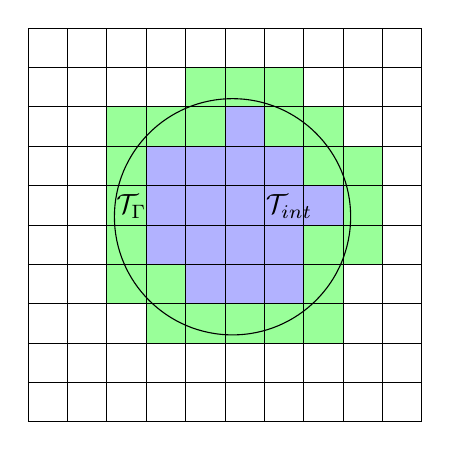
\begin{tikzpicture}[scale=1]

            % POTENTIAL ACTIVE MESH
            \fill[blue!30] (2,2) -- (2,-1.5) --(-1.5,-1.5) -- (-1.5,2) -- cycle;

            % ELEMENTS WITH NO INTERSECTION
            % lower left
            \fill[white] (-1.5,-1.5) rectangle (-1.0,-1.0);
            \fill[white] (-1.5,2.0) rectangle (-1.0,1.5);
            \fill[white] (-1.0,2.0) rectangle (-0.5,1.5);
            \fill[white] (2,2) rectangle (1.5,1.5);
            \fill[white] (1.5,2) rectangle (1.0,1.5);
            \fill[white] (2,1.5) rectangle (1.5,1.0);
            \fill[white] (1.5,-1) rectangle (2,-1.5);
            \fill[white] (1.5,-0.5) rectangle (2,-1.0);

            % CUT ELEMENTS
            \fill[green!40] (-0.5,2.0) rectangle (1.0,1.5);
            \fill[green!40] (-1.5,1.5) rectangle (0.0,1.0);
            \fill[green!40] (0.5,1.5) rectangle (1.5,1.0);
            \fill[green!40] (-1.5,1.0) rectangle (-1.0,-1.0);
            \fill[green!40] (-1.0,-0.5) rectangle (-0.5,-1.5);
            \fill[green!40] (-0.5,-1.5) rectangle (1.5,-1.0);
            \fill[green!40] (1.5,-1) rectangle (1.0,-0.0);
            \fill[green!40] (1.5,-0.5) rectangle (2.0,1.0);
            \fill[green!40] (1.0,0.5) rectangle (1.5,1.0);

            \draw (0.1, 0.1) circle (1.5cm);
            % Background mesh
            \foreach \i in {-2.5, -2, ..., 2.5} {
                \draw[line width=0.1pt, shift={(-2.5,\i)}] (0,0) -- (5,0);
                \draw[line width=0.1pt, shift={(\i,-2.5)}] (0,0) -- (0,5);
            }


            % Labels
            \node[below right] at (0.4,0.5) {$\mathcal{T}_{int}$};
            \node[below right] at (-1.5,0.5) {$\mathcal{T}_{\Gamma }$};
        \end{tikzpicture}
    \end{block}
\end{frame}

\begin{frame}
\frametitle{Cut Finite Element Method (CutFEM)}

A recent and promising numerical technique for PDEs, has gained significant momentum in the past decade \footnotemark[1]\footnotemark[2].

\begin{block}{}
    \begin{itemize}
        \item  Complex domains and moving domains efficiently.
        \item Utilizing so-called ghost penalties to ensure well-posedness.
        % \item Dividing the computational domains into \textbf{background} , \textbf{active}, \textbf{cut}  and \textbf{interior} mesh.
    \end{itemize}
\end{block}
\footnotetext[1]{\fullcite{burman2015cutfem}}
\footnotetext[2]{\fullcite{gurkan2019stabilized}}

\end{frame}




% \begin{frame}
% \frametitle{ Cut $C^0$ Interior penalty method (CutCIP) }

% \begin{block}{}
% The discretized numerical problem is to solve $w \in V_{h}$ such that
% \begin{equation*}
% \label{eq:CP_A_F}
% A( w, v )  = a_{h}( w,v) + \textcolor{red}{g_{h}( w,v)}  = l_{h}( v), \quad \forall v \in V_{h}  .
% \end{equation*}

% Where the additional bilinear term $g_{h}( w,v) : V_{h} \times V_{h} \to  \mathbb{R} $ is the so-called \textbf{ghost penalty}, which does the numerical regularization to ensure stability on cut cells.

% \end{block}

% \end{frame}

\begin{frame}
\frametitle{ CutCIP Method}

My master's thesis is dedicated to demonstrating that the relevant properties remain valid for CutCIP formulation still holds.

    \begin{block}{Well-posedness }
         The discrete bilinear form $a_{h}$ is wellposed on $V_{h}$ if this holds; \[
             \begin{split}
                 (Coercivity) \quad  A( v,v) &  \gtrsim  \| v \|_{A }^{ 2 } \quad  \forall v \in  V_{h} \\
            (Boundedness) \quad A( v,w) & \lesssim  \| v \|_{A }^{  }\| w \|_{a_{h} }^{  } \quad  \forall v,w \in  V_{h}
             \end{split}
        \]
    \end{block}

    \begin{block}{Apriori Estimates }

         Let $u$ be the solution to the strong problem with the corresponding discrete solution $u_{h}$ with polynomical order $k\ge 2$ .
        Then does it exist  $l = \min_{} ( 2, k)  $ s.t.
\[
        \| u - u_{h} \|_{a_{h}  }^{  } \lesssim  h^{l-1} \| u \|_{ H^{l} ( \Omega ) }^{  }
\]
    \end{block}
    % \footnotetext[1]{\fullcite{Gu2012}}
\end{frame}



\begin{frame}
\frametitle{ Cut $C^0$ Interior Penalty Method (CutCIP) Results }
% \frametitle{Manufactured Solution}


\begin{block}{Manufactured solution}
    In the experiments will we only consider polynomial order $k=2$.
We consider the manufactured solution:
$$
u_{ex}(\mathbf{x}) = \left(x_1^2 + x_2^2 - 1\right)^2 \cos(2\pi x_1) \cos(2\pi x_2)
$$
where $\mathbf{x}=(x_1,x_2)$ and $\Omega=\{(x_1,x_2): x_1^2 + x_2^2 \le  1\}$.
This manufactured solution can be used to test the accuracy of numerical methods for solving the above differential equation.
\end{block}
\end{frame}


\begin{frame}
\frametitle{ Cut $C^0$ Interior penalty method (CutCIP) Results }
\resizebox{\textwidth}{!}{
\begin{tabular}{rrrrrrrrr}
    \hline\hline
    \textbf{$n$} & \textbf{$\Vert e \Vert_{L^2}$} & \textbf{EOC} & \textbf{$ \Vert e \Vert_{H^1}$} & \textbf{EOC} & \textbf{$\Vert e \Vert_{ a_h,* }$} & \textbf{EOC} & \textbf{Cond number} & \textbf{ndofs} \\\hline
    4 & 2.4E+00 &  & 3.3E+00 &  & 6.2E+01 &  & 8.7E+04 & 8.1E+01 \\
    8 & 3.6E-01 & 2.72 & 1.1E+00 & 1.60 & 3.9E+01 & 0.68 & 5.1E+05 & 2.4E+02 \\
    16 & 2.2E-02 & 4.06 & 2.5E-01 & 2.12 & 1.4E+01 & 1.51 & 3.7E+06 & 8.3E+02 \\
    32 & 5.6E-03 & 1.97 & 6.0E-02 & 2.04 & 3.6E+00 & 1.93 & 2.8E+07 & 3.0E+03 \\
    64 & 1.4E-03 & 2.00 & 1.5E-02 & 2.02 & 9.2E-01 & 1.96 & 2.1E+08 & 1.1E+04 \\
    128 & 3.5E-04 & 2.00 & 3.7E-03 & 2.01 & 2.4E-01 & 1.94 & 1.7E+09 & 4.3E+04 \\\hline\hline
  \end{tabular}
}
\end{frame}






\begin{frame}
\frametitle{ Cut $C^0$ Interior penalty method (CutCIP) Results }

\begin{figure}[h!]
    \centering
    \resizebox{0.6\textwidth}{!}{% Recommended preamble:
% \usetikzlibrary{arrows.meta}
% \usetikzlibrary{backgrounds}
% \usepgfplotslibrary{patchplots}
% \usepgfplotslibrary{fillbetween}
% \pgfplotsset{%
%     layers/standard/.define layer set={%
%         background,axis background,axis grid,axis ticks,axis lines,axis tick labels,pre main,main,axis descriptions,axis foreground%
%     }{
%         grid style={/pgfplots/on layer=axis grid},%
%         tick style={/pgfplots/on layer=axis ticks},%
%         axis line style={/pgfplots/on layer=axis lines},%
%         label style={/pgfplots/on layer=axis descriptions},%
%         legend style={/pgfplots/on layer=axis descriptions},%
%         title style={/pgfplots/on layer=axis descriptions},%
%         colorbar style={/pgfplots/on layer=axis descriptions},%
%         ticklabel style={/pgfplots/on layer=axis tick labels},%
%         axis background@ style={/pgfplots/on layer=axis background},%
%         3d box foreground style={/pgfplots/on layer=axis foreground},%
%     },
% }

\begin{tikzpicture}[/tikz/background rectangle/.style={fill={rgb,1:red,1.0;green,1.0;blue,1.0}, fill opacity={1.0}, draw opacity={1.0}}, show background rectangle]
\begin{axis}[point meta max={nan}, point meta min={nan}, legend cell align={left}, legend columns={1}, title={}, title style={at={{(0.5,1)}}, anchor={south}, font={{\fontsize{14 pt}{18.2 pt}\selectfont}}, color={rgb,1:red,0.0;green,0.0;blue,0.0}, draw opacity={1.0}, rotate={0.0}, align={center}}, legend style={color={rgb,1:red,0.0;green,0.0;blue,0.0}, draw opacity={1.0}, line width={1}, solid, fill={rgb,1:red,1.0;green,1.0;blue,1.0}, fill opacity={1.0}, text opacity={1.0}, font={{\fontsize{8 pt}{10.4 pt}\selectfont}}, text={rgb,1:red,0.0;green,0.0;blue,0.0}, cells={anchor={center}}, at={(1.02, 1)}, anchor={north west}}, axis background/.style={fill={rgb,1:red,1.0;green,1.0;blue,1.0}, opacity={1.0}}, anchor={north west}, xshift={1.0mm}, yshift={-1.0mm}, width={94.6mm}, height={74.2mm}, scaled x ticks={false}, xlabel={$\delta$}, x tick style={color={rgb,1:red,0.0;green,0.0;blue,0.0}, opacity={1.0}}, x tick label style={color={rgb,1:red,0.0;green,0.0;blue,0.0}, opacity={1.0}, rotate={0}}, xlabel style={at={(ticklabel cs:0.5)}, anchor=near ticklabel, at={{(ticklabel cs:0.5)}}, anchor={near ticklabel}, font={{\fontsize{11 pt}{14.3 pt}\selectfont}}, color={rgb,1:red,0.0;green,0.0;blue,0.0}, draw opacity={1.0}, rotate={0.0}}, xmajorgrids={true}, xmin={-0.001471665988344504}, xmax={0.05052719893316125}, xticklabels={{$0.00$,$0.01$,$0.02$,$0.03$,$0.04$,$0.05$}}, xtick={{0.0,0.010000000000000002,0.020000000000000004,0.030000000000000006,0.04000000000000001,0.05000000000000001}}, xtick align={inside}, xticklabel style={font={{\fontsize{8 pt}{10.4 pt}\selectfont}}, color={rgb,1:red,0.0;green,0.0;blue,0.0}, draw opacity={1.0}, rotate={0.0}}, x grid style={color={rgb,1:red,0.0;green,0.0;blue,0.0}, draw opacity={0.1}, line width={0.5}, solid}, axis x line*={left}, x axis line style={color={rgb,1:red,0.0;green,0.0;blue,0.0}, draw opacity={1.0}, line width={1}, solid}, scaled y ticks={false}, ylabel={$\kappa(A)$}, y tick style={color={rgb,1:red,0.0;green,0.0;blue,0.0}, opacity={1.0}}, y tick label style={color={rgb,1:red,0.0;green,0.0;blue,0.0}, opacity={1.0}, rotate={0}}, ylabel style={at={(ticklabel cs:0.5)}, anchor=near ticklabel, at={{(ticklabel cs:0.5)}}, anchor={near ticklabel}, font={{\fontsize{11 pt}{14.3 pt}\selectfont}}, color={rgb,1:red,0.0;green,0.0;blue,0.0}, draw opacity={1.0}, rotate={0.0}}, ymode={log}, log basis y={10}, ymajorgrids={true}, ymin={100000.0}, ymax={1.0e25}, yticklabels={{$10^{5}$,$10^{10}$,$10^{15}$,$10^{20}$,$10^{25}$}}, ytick={{100000.0,1.0e10,1.0e15,1.0e20,1.0e25}}, ytick align={inside}, yticklabel style={font={{\fontsize{8 pt}{10.4 pt}\selectfont}}, color={rgb,1:red,0.0;green,0.0;blue,0.0}, draw opacity={1.0}, rotate={0.0}}, y grid style={color={rgb,1:red,0.0;green,0.0;blue,0.0}, draw opacity={0.1}, line width={0.5}, solid}, axis y line*={left}, y axis line style={color={rgb,1:red,0.0;green,0.0;blue,0.0}, draw opacity={1.0}, line width={1}, solid}, colorbar={false}]
    [\addlegendimage{empty legend}] \addlegendentry[font={{\fontsize{11 pt}{14.3 pt}\selectfont}}, text={rgb,1:red,0.0;green,0.0;blue,0.0}] {\hspace{-.6cm}{\textbf{$(\gamma, \gamma_1, \gamma_2)$}}}
    \addplot[color={rgb,1:red,0.0;green,0.0;blue,1.0}, name path={e73f70a5-bbbd-4a24-8407-eef9d08bc09d}, draw opacity={1.0}, line width={1}, solid]
        table[row sep={\\}]
        {
            \\
            0.0  1.2679164207221107e8  \\
            0.012263883236204186  1.2718633484176141e8  \\
            0.024527766472408372  1.2693944128424127e8  \\
            0.03679164970861256  1.2718633338545807e8  \\
            0.049055532944816745  1.2679164340263365e8  \\
        }
        ;
    \addlegendentry { $1.0 \cdot 10^{1}$, $0.5 \cdot 10^{1}$, $1.0 \cdot 10^{-1}$ }
    \addplot[color={rgb,1:red,1.0;green,0.0;blue,0.0}, name path={8dbacc37-3690-4b1f-9d5d-1b6f1fc900ac}, draw opacity={1.0}, line width={1}, solid]
        table[row sep={\\}]
        {
            \\
            0.0  4.639960110962716e10  \\
            0.012263883236204186  4.932252358128007e12  \\
            0.024527766472408372  4.0959531093983247e12  \\
            0.03679164970861256  4.932252223523245e12  \\
            0.049055532944816745  4.639960117645048e10  \\
        }
        ;
    \addlegendentry { $1.0 \cdot 10^{1}$, $ 0.0 \cdot 10^{0} $, $ 0.0 \cdot 10^{0} $ }
\end{axis}
\end{tikzpicture}
}
    \caption{The plot presents the $L^2$ and $H^1$ error norms and the error in the energy norm ($\Vert e \Vert_{a_h,*}$).}
    \label{fig:CutFEM_error1}
\end{figure}

\end{frame}

\begin{frame}
\frametitle{The Cahn Hilliard Equation}
    \begin{columns}
        % Left column
        \begin{column}{0.5\textwidth}
            \begin{block}{Recall}
                The problem has the form $u( x, t): \Omega \times [0,T] \mapsto [-1,1]$ s.t.
                \[
                \begin{split}
                    u_t+\Delta\left(\varepsilon \Delta u-\frac{1}{\varepsilon} f(u)\right)&=0 \quad \text{in } \Omega \\
                    \partial_n u=\partial_n \Delta u& =0 \quad \text{on } \Gamma  \\
                    u & =u_0 \quad \text{on } \Omega
                \end{split}
                \]
                where $f(u)$ is a nonlinear function.
            \end{block}
        \end{column}
        % Right column
        \begin{column}{0.5\textwidth}
            \begin{block}{Plan forward}
                \begin{enumerate}
                    \item We have now a tool to solve the $\Delta ( \Delta u) $ operator
                    \item Will utilize the time-iteration scheme to solve non-linearity
                \end{enumerate}
            \end{block}
        \end{column}
    \end{columns}
\end{frame}


\begin{frame}
\frametitle{The CutCIP Cahn-Hilliard Formulation}


Drawing upon the concepts delineated in Feng\footnotemark[1], the most efficient approach to address the nonlinear term is by employing an implicit-explicit (IMEX) scheme.

\begin{block}{IMEX method on the CutCIP formulation}
    Let $u^{m}_{h} \in V_{h}$ for the timesteps $m=0,1,\ldots,M$. Let $u_{h}^{0} = u_{0}$ be the initial timestep, then is.
\[
(\overline{\partial}  _{t} u_{h}^m, v_h ) + \varepsilon A (u_{h}^{m}, v_h )+\frac{1}{\varepsilon} c_h ( u_{h}^{m-1}, v_h)=0 \quad \forall v_h \in V_h^m .
\]
Here is $c_{h}( . , .) $ an the nonlinear terms handled in a implicit fashion. The $ \overline{\partial}  _{t}$ operator is simply a finite difference scheme in time-dimension.

\end{block}

\footnotetext[1]{\fullcite{feng2007fully}}
\end{frame}

\begin{frame}
\frametitle{The CutCIP Cahn-Hilliard Experiments}
Implemented using the Gridap FEM framework written in Julia \footnotemark[1].


\begin{block}{Simulation parameters}
    \begin{itemize}
        \item Physical domain $\Omega$  is a 4 discs of radius $R=1$ with distance $d=0.999$, i.e. they are touching!
        \item Inital data is $u_0 = random(-1,1)$ in physical domain $\Omega $.
        % \item Backgroundmesh with size ($L\times L$ ) for $L=2$ and $n=128$.
        % \item Polynomial order $k=2$ .
        % \item Physical parameter $\varepsilon  = \frac{1}{30}$.
        % \item Time-step $\tau = \varepsilon ^{2} \frac{1}{10} $ for the interval $ 0\le t \le 10^3 \tau $.
    \end{itemize}
\end{block}

\footnotetext[1]{\fullcite{badia2020gridap}}


\end{frame}

\begin{frame}
\frametitle{The CutCIP Cahn-Hilliard Experiments}

\begin{figure}[h]
    \centering
    \includegraphics[width=0.5\textwidth]{CH-example/0.png}
    \caption{Iteration 0}
    \label{fig:your_image_label}
\end{figure}
\end{frame}

\begin{frame}
\frametitle{The CutCIP Cahn-Hilliard Experiments}

\begin{figure}[h]
    \centering
    \includegraphics[width=0.5\textwidth]{CH-example/1.png}
    \caption{Iteration 1}
\end{figure}
\end{frame}

\begin{frame}
\frametitle{The CutCIP Cahn-Hilliard Experiments}
\begin{figure}[h]
    \centering
    \includegraphics[width=0.5\textwidth]{CH-example/10.png}
    \caption{Iteration 10}
\end{figure}
\end{frame}

\begin{frame}
\frametitle{The CutCIP Cahn-Hilliard Experiments}
\begin{figure}[h]
    \centering
    \includegraphics[width=0.5\textwidth]{CH-example/50.png}
    \caption{Iteration 50}
\end{figure}
\end{frame}

\begin{frame}
\frametitle{The CutCIP Cahn-Hilliard Experiments}
\begin{figure}[h]
    \centering
    \includegraphics[width=0.5\textwidth]{CH-example/200.png}
    \caption{Iteration 200}
\end{figure}
\end{frame}

\begin{frame}
\frametitle{The CutCIP Cahn-Hilliard Experiments}
\begin{figure}[h]
    \centering
    \includegraphics[width=0.5\textwidth]{CH-example/1000.png}
    \caption{Iteration 1000}
\end{figure}
\end{frame}


\begin{frame}
\frametitle{Further work}
\begin{enumerate}
    \item Adaptive time steps.
    \item Further numerical validation.
    \item Extend the method to handle moving domains.

\end{enumerate}
\end{frame}


\begin{frame}
\frametitle{Questions?}
\end{frame}



    %%% old
    % 
\section{Mathematical Background}%
\label{sec:mathematical_background}

We will in this section will we review standardized and well know methods and notations. Generally is the notation followed from \cite[Chapter 1]{pietro2012}.


\subsection{Notation}%
\label{sub:notation}

We will in this report assume $\Omega $ to be a compact and open set in $\mathbb{R} ^{d}$. Let $p \in \mathbb{R} $, $ 1 \le  p \le  \infty$, and  define the space $L^{p}\left( \Omega  \right) $ to be the set of all measurable functions $u: \Omega  \mapsto \mathbb{R} $ such that
$\left\lvert f \right\rvert ^{p}$ is Lebesgue integrable, i.e,

\begin{equation*}
    L^{p}\left( \Omega  \right) = \left\{ u: \Omega \mapsto \mathbb{R}  \mid \int_{\Omega }^{} \left\lvert u \right\rvert ^{p} d \Omega  < \infty  \right\}
.\end{equation*}
Let $u \in L^{p}\left( \Omega  \right) $. We define the integral norm of order $p$ to be \[
\| u \|_{ L^{p}\left( \Omega  \right)  }^{  }  = \left( \int_{\Omega }^{} \left\lvert u \right\rvert ^{p} dx  \right) ^{\frac{1}{p}}.
\]
Since $p=2$ is frequently used in this report, we also define for convenience a compact notation $\| u \|_{ \Omega  }^{  }  = \| u \|_{ L^{2}\left( \Omega  \right)  }^{  } $ .  Recall that $L^{2}\left( \Omega  \right) $ is a Hilbert space if it is equipped with a inner
product of two functions $u,v \in L^{2}\left( \Omega  \right) $ such that
    $
\left( u,v \right) _{\Omega } = \left( u,v \right) _{L^2\left( \Omega  \right) } = \int_{\Omega }^{} u  v dx.
$
The following definition for derivatives is employed,
\begin{equation}
\label{eq:mixed_derivative}
\partial ^{\alpha  } u = \frac{\partial ^{\left\lvert \alpha  \right\rvert } u}{ \partial ^{\alpha _{1} } x_{1} \partial ^{\alpha _{2}} x_{2}  }, \quad \text{for } \alpha=\left( \alpha _{1}, \alpha _{2} \right) \text{ and } f \in C^{\left\lvert \alpha  \right\rvert }
\left( \Omega  \right)
.\end{equation}
For $d$ dimensions of order $k$ we define the multi-index $\alpha  = ( \alpha _{1}, \ldots, \alpha _{d})  $ with the absolute value $\abs{ \alpha  } = \sum_{i=1}^{d}  \alpha _{i} = k $ s.t.
\[
\partial ^{\alpha} u = \frac{\partial ^{ \alpha_{1}  }  } {\partial^{} x_{1}^{\alpha _{1}}  } \ldots \frac{\partial ^{ \alpha_{d}  }  } {\partial^{} x_{d}^{\alpha _{d}}  } u
\]

  Let $m\ge 0$ be an integer and let $1 \le  p \le  \infty$ be a real number. Then the Sobolev space $H^{m}( \Omega ) $ are defined by
\[
H^{m}\left( \Omega  \right) = \left\{ u \in L^{2}\left( \Omega  \right)  \mid  \partial ^{\alpha } u \in L^{2}\left( \Omega  \right)  \forall \alpha : \left\lvert \alpha  \right\rvert  \le m \right\}.
\]
Equipped with the inner product for $u,v \in H^{m}\left( \Omega  \right) $, \[
    \left( u,v \right) _{H^{m}\left( \Omega   \right) } = \sum_{\left\lvert \alpha  \right\rvert  \le  m}^{}  \int_{\Omega }^{} \partial ^{\alpha } u \partial ^{\alpha } v dx,
\]
with the corresponding norm
$
\| u \|_{ H^{m}\left( \Omega  \right)  }^{2  }  =  \| u \|_{ L^{2}\left( \Omega  \right)    }^{2} + \sum_{k = 1}^{m}  \left\lvert u \right\rvert ^{2} _{  H^{k}\left( \Omega  \right) }.
$
Here the seminorm is defined such that, $ \left\lvert u \right\rvert _{H^{k}( \Omega  ) }^{2} =  \sum_{\left\lvert \alpha  \right\rvert  = k}^{} \| \partial ^{\alpha }u \|_{ \Omega  }^{ 2 }  .
$
We will often use the shorthand notation $ \| u \|_{ k, \Omega  }^{  } = \| u \|_{ H^{k}( \Omega)  }^{  } $ and $ \abs{ u }_{ k, \Omega  }^{  }  = \abs{ u }_{ H^{k}( \Omega)  }^{  }$.

Given the context of Sobolev spaces, we consider the functions $ u \in H^{2}( \Omega )$ and $ v \in H^{1}( \Omega )$. We can denote Greens theorem, which links integrals over a volume and its boundary, as follows,
\[
( \Delta u, v) _{\Omega } = -( \nabla u, \nabla v)_{\Omega } + ( u, \partial _{n}v)_{\Gamma }
\]
This identity serves as an essential tool for the calculations done.



\subsection{Computational Domains}%
\label{sub:computational_domain}
Assume that $\Omega \subset \mathbb{R} ^{d} $ is a compact set with a boundary  $\Gamma $. In standard FEM methods a key assumption is that the set $\Omega $ is a polyhedra. This is useful since a polyhedra can be fully covered by a collection of polyhedra and, hence, motivating us to define a fitted mesh.
We define a fitted mesh $\mathcal{T} $ of the domain $\Omega $ to be a collection of disjoint polyhedra $\left\{ T \right\}  $ forming a partition of $\Omega $ s.t $\overline{\Omega } = \bigcup _{T \in \mathcal{T} } T $, for illustration see Figure
\ref{fig:domain_mesh}.
Here we say that each $T \in  \mathcal{T} $ is a mesh element or an element.
The mesh size is defined as the maximum diameter $h := h_{max} $ of any polyhedra in the mesh $\mathcal{T} = \left\{ T \right\}  $, that is, $ h_{max} = \max_{T \in \mathcal{T} }  h_{T}$ s.t.
$h _{T}  = \mathrm{diam}\left( T \right)   = \mathrm{max}_{x_1, x_{2} \in T} \ \mathrm{ dist }(x_{1}, x_{2})$
Hence, motivating us to use the notation $\mathcal{T} _{h}$ for a mesh $\mathcal{T} $ with size $h$.

For simplicity will we restrict ourself to simplicial and quadrilateral elements.
A mesh $\mathcal{T}_{h}$ in $ \mathbb{R} ^{d}$ is said to be matching if
for all neighbouring elements $T_{1}, T_{2} \in \mathcal{T} _{h}$ such that the intersection $T_{1} \cap T_{2} $ is a manifold of dimensions $( d-1)$, then $T_{1} \cap T_{2} $ a entire facet of both $T_{1}$ and $T_{2}$.

Let the chunkiness parameter $c_{T} := h_{T}/r_{T}$, where $r_{T}$  is the largest ball that be inscribed inside a element $T \in \mathcal{T}_{h} $.
A mesh is said to be shape regular if $c_{T}\le  c$ is independent of $T$  and $h$. We also say that the mesh is quasi-uniform only if it is shape regular and $h_{\mathrm{ max }} \le  c h_{\mathrm{ min }}$.
For a more complete description of meshes, see \cite[Chapter 8]{ErnGuermond2021}.

In this thesis will we assume that a mesh $\mathcal{T}_{h} $ is matching, shape regular and quasi-uniform unless specified.
 The fact that the mesh is conform makes is a useful property since the interface between mesh elements has come into contact in the sense
that it is either a vertex or a facet. This with the combination of shape regularity and quasi-uniformity is a major key to prove important inequalities in broken Sobolev spaces \cite[Chapter 1.4.1]{pietro2012}. Hence, the assumptions are very handy when proving convergence.


Let $\mathcal{T}_{h}  = \left\{ T \right\} $ be a mesh of $\Omega \subset  \mathbb{R} ^d $ consisting of polygons $T \in \mathbb{R} ^{d}$.
The set of all facets is the union of external and internal facets, $\mathcal{F} _{h} = \mathcal{F} ^{ext}_{h} \cup \mathcal{F} _{h}^{int} $, where each are defined by
\[
            \mathcal{F}^{int} _{h}  = \left\{ F=T^{+}\cap T^{-}  \mid  T^{+}, T^{-} \in \mathcal{T}_{h}  \right\} \text{ and }
            \mathcal{F}^{ext} _{h}  = \left\{ F= \partial T \cap \partial \Omega    \mid  T  \in \mathcal{T}_{h}  \right\}.
\]
Assume $T^{+} \neq T^{-}$ . Next, we define the following normal vectors.
\begin{enumerate}[label=\arabic*)]
    \item We define $ n= n  _{\partial T}$ to be unit outward normal on $\partial T$ for each $T \in \mathcal{T}_{h} $
\item Let $F \in \mathcal{F }^{int} _{h}$. We define $n$ to be the facet normal $ n =  n _F = n | _{\partial T^{+}} $  from $T^{+}$ to $T^{-}$, illustrated in Figure \ref{fig:normal}. \red{Ask Andre about his comment here.}
 \item Let $F \in \mathcal{F} ^{ext}_{h}$. Then we define the facet normal $n | _{F} = n | _{\partial T} $ to be the unit outward normal.
\end{enumerate}
Please note that we for convenience employ the notation $n$ when it is clear what entity the normal is associated with.

    Let $v\in L^2( \Omega ) $ be a scalar function on $\Omega$ with a corresponding shape regular and quasi-uniform mesh $\mathcal{T}_{h} $. We will use the following definitions.
    \begin{enumerate}[label=\arabic*)]
        \item Let $F \in \mathcal{F}^{int} _{h}$ and $v^{\pm}| _{F} = \lim_{t\to 0^{+}} v( x \mp tn)   $ for $x \in F$. We define the mean as $\mean{ v} |_{F} = \frac{1}{2} (v^{+}_{F} + v^{-}_{F})   $ and the jump as $\jump{v}|_{F} =  v^{+}_{F} - v^{-}_{F} $.
        \item Let $F \in \mathcal{F}^{ext} _{h}$ and let $ v( x) =  v(x)|_{F} $ for  $x \in F$.
We define the mean as $\mean{ v} |_{F} = v    $ and the jump as $\jump{v}|_{F} = v$.

    \end{enumerate}
    To simplify will we use the notation $\mean{ v } = \mean{ v }|_{F}    $ and $\jump{ v } = \jump{ v }| _{F}    $ for all $F \in \mathcal{F} _{h}$.
    Remark that if we have two functions $u,v$, for which $u^{\pm}( x) $ and $v^{\pm}( x) $ are defined, then the following identity holds $  \jump{ uv }    = \jump{ u }   \mean{ v }    + \mean{ u }  \jump{ v }$ along all facets $ \mathcal{F}_{h} $ associated with the
    triangulation $\mathcal{T} _{h}$.


\begin{figure}[h!]
\centering
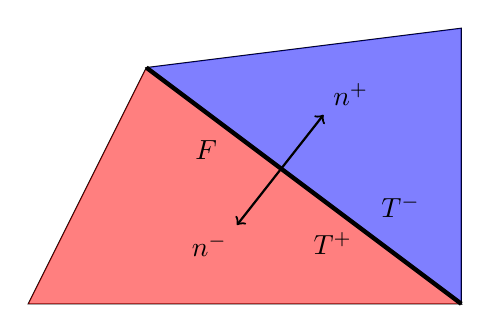
\begin{tikzpicture}[scale=1]
\coordinate (A) at (-1.5, -0);
\coordinate (C) at (0,3);
\coordinate (B) at (4,0);
\coordinate (D) at (4,3.5);

\draw (A) -- (B) -- (C) -- cycle;
\draw (B) -- (C) -- (D) -- cycle;
\fill[red, opacity=0.5] (A) -- (B) -- (C);
\fill[blue, opacity=0.5] (B) -- (C) -- (D);
\draw[ultra  thick] (C) -- (B);

\coordinate (Tm) at (3.6,1.5);
\coordinate (Tp) at (2.0, 0.5);
\coordinate (e) at (0.5, 2.2);
\node[below left] at (Tm) {$T^{-} $ };
\node[above right] at (Tp) {$T^{+}$ };
\node[below right] at (e) {$F$ };

\coordinate (start) at (1.7, 1.7);
\coordinate (endPlus) at (2.25, 2.4);
\coordinate (endMinus) at (1.15, 1.0);

\draw [->, thick] (start) -- (endPlus);
\node[above right] at (endPlus) {$n^{+}$};

\draw [->, thick] (start) -- (endMinus);
\node[below left] at (endMinus) {$n^{-}$};

\end{tikzpicture}

\caption{Facet $F \in \mathcal{F}_h^{int} $ shared by the triangles $T^{+}, T^{-} \in \mathcal{T}_{h} $ and the normal unit vector $n^{+}$ and $n^{-}$. If we pick $T=T^{+}$ and want to evaluate the normal vector $n$ along a facet $F$, then we define $n = n  \mid _{F} = n^{+}$.}
    \label{fig:normal}
\end{figure}



\subsection{Broken Sobolev spaces}%
\label{sub:broken_sobolev_spaces}

In this work will we compute norms on discontinuous elements, thus, it will be necessary to define broken Sobolev spaces.
Let $\mathcal{T}_{h} $ be a mesh and some integer $m\le n$. Then we define the broken Sobolev space to be \[
    \begin{split}
H^{m}( \mathcal{T}_{h} ) & := \left\{ v \in L^2( \Omega )  \mid \ v|_{T} \in H^{m}( T) \quad     \forall T \in  \mathcal{T} \right\}\\
        L^{2}( \mathcal{F}_{h} ) &:= \left\{ v \in L^2( \mathcal{T}_{h}  )  \mid   \ v|_{F} \in L^{2}( F)  \quad  \forall F \in  \mathcal{F}_{h}   \right\}.
    \end{split}
\]
This motivates us to define broken Sobolev norms and inner products using summation over mesh elements,
\[
 \| v \|_{H^{m}( \mathcal{T}_{h} ) }^{2} = \sum_{T \in  \mathcal{T}_{h} }^{} \| v  \|_{ H^{m}( T ) }^{2  } \quad \text{ and } \quad
 (v ,w )_{H^{m}( \mathcal{T}_{h} ) }^{} = \sum_{T \in \mathcal{T} _{h}}^{} (v ,w )_{ H^{m}( T ) }^{  } .
\]
As before, we use the shorthand notation,  $\| v \|_{\mathcal{T}_{h}} =  \| v \|_{L^{2}( \mathcal{T}_{h} ) }$ and  $(v ,w )_{ \mathcal{T}_{h} }^{} = (v ,w )_{L^2( \mathcal{T}_{h} ) }^{} $.
That is,
\[
 \| v \|_{L^{2}( \mathcal{F}_{h} ) }^{2} = \sum_{F \in  \mathcal{F}_{h} }^{} \| v  \|_{ L^{2}( F ) }^{2  } \quad \text{ and } \quad
 (v ,w )_{L^{2}( \mathcal{F}_{h} ) }^{} = \sum_{T \in \mathcal{F} _{h}}^{} (v ,w )_{ L^{2}( F ) }^{  } .
\]
Again, we often use the more compact notation $\| v \|_{\mathcal{F}_{h}} =  \| v \|_{L^{2}( \mathcal{F}_{h} ) }$ and  $(v ,w )_{ \mathcal{F}_{h} }^{} = (v ,w )_{L^2( \mathcal{F}_{h} ) }^{} $.
A very useful lemma when working with estimates on broken Sobolev spaces is that a if a function is continuous, then the jump between the mesh elements is zero. A function $ v \in  H^{1}( \mathcal{T}_{h} ) $ belongs to $ H^{1}( \Omega )  $ if and only
if $ \jump{ v }   = 0 \text{ for }  F \in \mathcal{F}^{int}_{h}$.



\subsection{Useful inverse estimates}%
\label{sub:useful_inverse_estimates}

We first some the standard inequalities.
\begin{enumerate}[label=(\roman*)]
    \item A fundamental property of the inner-product the so-called Cauchy-Schwarz inequality
    \[
     ( u,v)_{H^{m}( \Omega )  }   \le \| u \|_{H^{m}( \Omega )   }^{  } \| v \|_{H^{m}( \Omega )    }^{  } \forall u,v \in H^{m}( \Omega )
    \]

    \item For any $a,b >\mathbb{R} $ the well known Youngs $\varepsilon $-inequality is on the form,
        \[
            2ab \le \varepsilon a^2+ \frac{1}{\varepsilon } b^2.
        \]
\end{enumerate}

Choose any triangle $T \in \mathcal{T}_{h} $ and let $v \in \mathcal{P}( T)  $. Then does the local inverse estimate hold,
$$
\abs{ v }_{H^{l}( T) } \lesssim h^{m-l} \abs{ v }_{H^{m}( \Omega ) }.
$$
for $l \le m$. For proof, see \cite[Lemma 12.1]{ErnGuermond2021}. An essential example is the following inequality.
$$\| D^2v \|_{T  }^{ 2 } \lesssim h^{-1} \| \nabla v  \|_{ T  }^{  } \lesssim h^{-2} \| v \|_{T  }^{  }   $$

Another very useful inequality is the so-called trace inequality which connect the relationship of evaluating the norm on element $ T $ and with any of the corresponding facets $F \in \partial T$. The general form is $\| v \|_{F   }^{  }  \lesssim
h^{-\frac{1}{2}} \| v \|_{ T  }^{  } $, see \cite[Lemma 12.8]{ErnGuermond2021}.
Let $\partial _{n} v = \nabla v \ n$ and $\partial_{nn} v = n^{T} D^2 v \ n $, and keeping in mind that the normal vector has a unit length, can we evidently apply the trace inverse inequality to conclude, \[
\begin{split}
    \| \partial _{n} v \|_{F  }^{  }  & \le \| \nabla v \|_{F  }^{  }  \le h^{-\frac{1}{2}} \| \nabla  v \|_{T  }^{  },  \\
    \| \partial _{nn} v \|_{ F }^{  } & \le  \| D^2 v \|_{ F }^{  }   \le  h^{-\frac{1}{2}} \| D^2 v \|_{ T }^{  }.
\end{split}
\]

% \begin{enumerate}[label=(\roman*)]
%     \item General inverse inequality.
%     Let $\alpha = ( \alpha _{1}, \ldots, \alpha _{N}) $ and $\beta = ( \beta _{1}, \ldots, \beta _{N} ) $.
%     Assume $u \in H^{\abs{ \beta  }  }( T) $. The following inverse inequalities hold.
%     \[
%         \begin{split}
%         \| \partial ^{\alpha } u \|_{T  }^{  } & \lesssim h^{ - \abs{ \beta  }  } \| \partial ^{\alpha - \beta } u \|_{T }^{  } \\
%         \| \partial ^{\alpha }_{n} u  \|_{F  }^{  } &\lesssim h^{-\frac{1}{2}  } \| \partial ^{\alpha } u \|_{T }^{  }
%         \end{split}
%     \]
% \end{enumerate}
    % For a full triangle we have \[
    % \| v \|_{ \partial T }^{  } \lesssim h_{T}^{-\frac{1}{2}} \| v \|_{ T }^{  } + h_{T}^{\frac{1}{2}} \| \nabla v \|_{ T }^{  }
    % \]




\subsection{Lax-Milgram lemma}%
\label{sub:lax_milgram_lemma}


\begin{definition}[Linear bounded functional]
    \label{def:linear_function}
Let $X$ be a Hilbert space. Furthermore, we define the dual space $X' $ to be the space of linear and bounded functionals $F: X  \mapsto \mathbb{R} $, i.e., \[
X'  = \left\{ F: X \to \mathbb{R}   \mid  F \text{ is linear and bounded} \right\}
\]
\end{definition}

\begin{problem}[Abstract linear problem]
    \label{def:abstract_linear_problem}
    Assume $X$ and $Y$  to be two Hilbert spaces. Let the vector space $\mathcal{L}( X,Y)  $ be all linear bounded operators spanned from $X$ to $Y$. We define the abstract linear problem as follows; find $u \in X$ s.t. \[
    a( u,v)  = l(v ) := \left<f,v \right>_{X' , X}  \forall v \in X
    \]
    Where $a \in  \mathcal{L} ( X, X,\mathbb{R} ) $ is a bounded bilinear form and $f \in X':= \mathcal{L} ( X,\mathbb{R} )  $ is a bounded linear form. Here we denote by $\left<\cdot ,\cdot  \right>_{X' .X} $ the duality pairing between $X' $ and $X $.

\end{problem}


\begin{definition}[Coercivity and Boundedness]
    \label{def:coercivity}
    Let $X$ be a Hilbert space and let $a( \cdot ,\cdot )  \in  \mathcal{L} ( X, X,\mathbb{R} )  $. Recall that the bilinear form $a( \cdot ,\cdot ) $ is coercive on $X$ if there exists an constant $C_{1} > 0 $ such that \[
     a( v,v) \ge  C_{2} \| v \|_{ X }^{  } \quad  \forall v \in  X
    \]
     The bilinear form $a( \cdot ,\cdot ) $ is said to bounded if there exists an constant $C_{2}$  \[
    a( u,v)  \le C_{1} \| u \|_{ X }^{  }  \| v \|_{X }^{  }
    \]
\end{definition}


\begin{lemma}[Lax-Milgram]
    \label{def:lax-milgram}
    The abstract linear problem \ref{def:abstract_linear_problem} is well-posed if $a(\cdot , \cdot  ) $ is bounded and coercive. Moreover, the following a priori estimate holds true.\[
    \| v \|_{ X }^{  } \lesssim  \| f \|_{ X'  }^{  }
    \]
\end{lemma}
\begin{proof}
    The problem can easily be proved using a special case of the Banach–Nečas–Babuška theorem. See \cite[Lemma 1.4]{pietro2012}
\end{proof}



\subsection{Finite element method}%
\label{sub:finite_element_method}


The finite element method (FEM) is a numerical method to solve partial differential equation by finding an approximation of the Problem \ref{def:abstract_linear_problem}.  Let $X_{h}$ be a finite-dimensional (polynomial) approximation space on the mesh
$\mathcal{T} _{h}$. We say that a method is conform if $X_{h}\subset X $ and non-conform if $X _{h} \not\subset X$. We define the approximate problem as follows.
\begin{problem}[The approximate problem]
    \label{def:approx_problem}
    Find  $u \in X_{h}$ s.t. \[
    a_{h}(u,v ) = \left<f,v \right>   \forall v \in X_{h}
    \]
\end{problem}

We denote the functional $a_{h}: X_{h} \times X_{h} \to \mathbb{R} $ as an consistent approximation of $a: X \times X \to \mathbb{R} $, and similarly for the right-hand side.
In this report will we generally specify any discrete space $X_{h}(\mathcal{T}_{h})$  as the $C^{0}$ continuous polynomial space $\mathcal{P}^{k}(\mathcal{T}_{h})$, of order $k$.

\begin{definition}[Broken polynomial spaces]
    Let $\mathcal{T}_{h} $ be a mesh of $\Omega \in \mathbb{R} ^{d} $. Let $\mathcal{P}^{k}(T) $ be the space of all polynomials of order $k$ in the mesh element $T$ in $\mathcal{T}_{h}$ . We define the broken polynomial space as \[
    \mathcal{P}^{k} ( \mathcal{T}_{h} ) := \left\{ v \in L^{2}( \mathcal{T}_{h} )    \mid  v|_{T} \in \mathcal{P}^k( T) \quad  \forall T \in  \mathcal{T}_{h}   \right\}.
    \]
    Similarly, the global $C^{0}$ continuous polynomial space is denoted as
    \[
    \mathcal{P}^{k}_{c} ( \mathcal{T}_{h} ) := \left\{ v \in C^{0}( \Omega )   \mid  v|_{T} \in \mathcal{P}^k( T) \quad  \forall T \in  \mathcal{T}_{h}   \right\}.
    \]

\end{definition}

\begin{definition}[Local polynomial space]
    \label{def:local_space}
    Let $T$ be a element in a mesh $\mathcal{T}_{h} $,  $x = \left[ x_{1}, \ldots, x_{d} \right] $ be a vector, and $\alpha  = \left[ \alpha _{1}, \ldots, \alpha _{d} \right] $ be a multi index.
    The local polynomial space $\mathcal{P} ^{k}( T) $ is denoted as
    \begin{equation}
    \label{eq:pol_space}
        \mathcal{P}^{k}( T) =  \mathrm{span}\left\{ x^{\alpha } \ \text{for } x \in T \text{ and } 0 \le  \alpha _{i} \le k \right\}.
    \end{equation}
    where  $x^{\alpha }$ is a monomial such that $x^{\alpha } = x_{1}^{\alpha _{1}} \ldots x_{d}^{\alpha _{d}}$.

\end{definition}

Following Ciarlet \cite[pp.93]{ciarlet1991basic}, the abstract definition of a finite element is defined as the triplet $( T, \mathcal{P}, \Sigma ) $. In our case is $T$ a simplex or a quadrilateral geometry and the $\mathcal{P} $ a finite dimensional polynomial space consisting of $N$ shape
functions $\left\{ \phi_{i}  \right\}_{i\in N} $ such as \eqref{eq:pol_space}.
On the other hand, $\Sigma $ is the so-called dual of $\mathcal{P}$, that is, the set of linear forms $\left\{ \sigma _{i} \right\} $ such that. $ \sigma_{j} ( \phi_{i} ) = \delta _{ij}$ and $p( x) = \sum_{i\in N}^{} \sigma_{i} ( p) p_{i} $.

If there is a set of points $\left\{ a_{i} \right\}_{i \in N} $  in $T$ such that
$\sigma_{i}( p) = p( a_{i}) \  \forall p \in \mathcal{P}$,  then the triple $( T, \mathcal{P}, \Sigma  ) $ is called a Lagrangian finite element. The set of points $\left\{ a_{i} \right\}_{i \in N}  $ is called nodes and is associated with the
so-called nodal basis of $\mathcal{P} $ such that  $\phi ( a_{i}) = \delta _{ij} \ \forall i,j  \in N$
As anticipated, the node configuration of the polynomial space, denoted as $\mathcal{P}^{k}( T)$, is influenced by the form of $T$. For the purpose of our discussion, let us represent the polynomial basis for a simplicial element and a quadrilateral
element as $\mathbb{P} ^{k}(T )$ and $\mathbb{Q} ^{k}( T)$, both of polynomial order $k$. In Figure \ref{fig:ill_nodes} is it illustrated for  $k=1,2,3$ in dimension $d=2$ on how the node configuration evolve.


\begin{figure}[hb!]
    \centering
    \hfill
    \subfloat[$\mathbb{P}^{1}( T)  $]{
        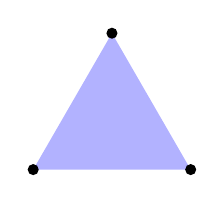
\begin{tikzpicture}[scale=1.0]
            % Define the coordinates
            \coordinate (A) at (0,0);
            \coordinate (B) at (2,0);
            \coordinate (C) at (1,{sqrt(3)});

            % Draw the triangle
            \fill[blue!30] (A) -- (B) -- (C) -- cycle;

            % Draw the nodes
            \fill (A) circle (2pt);
            \fill (B) circle (2pt);
            \fill (C) circle (2pt);
        \end{tikzpicture}
    }
    \hfill
    \subfloat[ $\mathbb{P}^{2}( T)  $]{
        \begin{tikzpicture}[scale=1.0]
            % Define the coordinates
            \coordinate (A) at (0,0);
            \coordinate (B) at (2,0);
            \coordinate (C) at (1,{sqrt(3)});

            % Define the midpoints
            \coordinate (D) at ($(A)!0.5!(B)$);
            \coordinate (E) at ($(B)!0.5!(C)$);
            \coordinate (F) at ($(A)!0.5!(C)$);

            % Draw the triangle
            \fill[blue!30] (A) -- (B) -- (C) -- cycle;

            % Draw the nodes
            \fill (A) circle (2pt);
            \fill (B) circle (2pt);
            \fill (C) circle (2pt);
            \fill (D) circle (2pt);
            \fill (E) circle (2pt);
            \fill (F) circle (2pt);
        \end{tikzpicture}
    }
    \hfill
    \subfloat[$\mathbb{P} ^{3}( T)  $ ]{
        \begin{tikzpicture}[scale=1.0]
            % Define the coordinates
            \coordinate (A) at (0,0);
            \coordinate (B) at (2,0);
            \coordinate (C) at (1,{sqrt(3)});

            % Define the additional points along the edges
            \coordinate (D) at ($(A)!0.3333!(B)$);
            \coordinate (E) at ($(B)!0.3333!(C)$);
            \coordinate (F) at ($(C)!0.3333!(A)$);
            \coordinate (G) at ($(A)!0.6667!(B)$);
            \coordinate (H) at ($(B)!0.6667!(C)$);
            \coordinate (I) at ($(C)!0.6667!(A)$);

            % Define the centroid
            \coordinate (J) at (1, {sqrt(3)/3});

            % Draw the triangle
            \draw (A) -- (B) -- (C) -- cycle;
            \fill[blue!30] (A) -- (B) -- (C) -- cycle;

            % Draw the nodes
            \fill (A) circle (2pt);
            \fill (B) circle (2pt);
            \fill (C) circle (2pt);
            \fill (D) circle (2pt);
            \fill (E) circle (2pt);
            \fill (F) circle (2pt);
            \fill (G) circle (2pt);
            \fill (H) circle (2pt);
            \fill (I) circle (2pt);
            \fill (J) circle (2pt);
        \end{tikzpicture}
    }
    \\
    \hfill
    \subfloat[$\mathbb{Q}^{1}( T)  $]{
        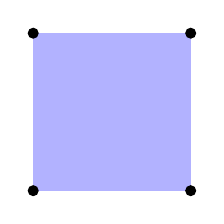
\begin{tikzpicture}[scale=1.0]
            % Define the coordinates
            \coordinate (A) at (0,0);
            \coordinate (B) at (2,0);
            \coordinate (C) at (2,2);
            \coordinate (D) at (0,2);

            % Draw the square
            \fill[blue!30] (A) -- (B) -- (C) -- (D) -- cycle;

            % Draw the nodes
            \fill (A) circle (2pt);
            \fill (B) circle (2pt);
            \fill (C) circle (2pt);
            \fill (D) circle (2pt);
        \end{tikzpicture}
    }
    \hfill
    \subfloat[ $\mathbb{Q} ^{2}( T)  $]{
        \begin{tikzpicture}[scale=1.0]
            % Define the coordinates
            \coordinate (A) at (0,0);
            \coordinate (B) at (2,0);
            \coordinate (C) at (2,2);
            \coordinate (D) at (0,2);

            % Define the midpoints
            \coordinate (E) at ($(A)!0.5!(B)$);
            \coordinate (F) at ($(B)!0.5!(C)$);
            \coordinate (G) at ($(C)!0.5!(D)$);
            \coordinate (H) at ($(D)!0.5!(A)$);
            % Define the centroid
            \coordinate (M) at (1, 1);

            % Draw the square
            \fill[blue!30] (A) -- (B) -- (C) -- (D) -- cycle;

            % Draw the nodes
            \fill (A) circle (2pt);
            \fill (B) circle (2pt);
            \fill (C) circle (2pt);
            \fill (D) circle (2pt);
            \fill (E) circle (2pt);
            \fill (F) circle (2pt);
            \fill (G) circle (2pt);
            \fill (H) circle (2pt);
            \fill (M) circle (2pt);
        \end{tikzpicture}
    }
    % And so on for $\mathcal{P}^{3}( S)  $, $\mathcal{P}^{4}( S)  $, etc.
    \hfill
    \subfloat[ $\mathbb{Q} _{3}( T)  $]{
        \begin{tikzpicture}[scale=1.0]
            % Define the coordinates
            \coordinate (A) at (0,0);
            \coordinate (B) at (2,0);
            \coordinate (C) at (2,2);
            \coordinate (D) at (0,2);

            % Define the additional points along the edges
            \coordinate (E) at ($(A)!0.3333!(B)$);
            \coordinate (F) at ($(B)!0.3333!(C)$);
            \coordinate (G) at ($(C)!0.3333!(D)$);
            \coordinate (H) at ($(D)!0.3333!(A)$);
            \coordinate (I) at ($(A)!0.6667!(B)$);
            \coordinate (J) at ($(B)!0.6667!(C)$);
            \coordinate (K) at ($(C)!0.6667!(D)$);
            \coordinate (L) at ($(D)!0.6667!(A)$);

            % Define the internal nodes
            \coordinate (M) at ($(E)+(0,0.6667)$);
            \coordinate (N) at ($(E)+(0,1.332)$);
            \coordinate (O) at ($(I)+(0,0.6667)$);
            \coordinate (P) at ($(I)+(0,1.332)$);

            % Draw the square
            \draw (A) -- (B) -- (C) -- (D) -- cycle;
            \fill[blue!30] (A) -- (B) -- (C) -- (D) -- cycle;

            % Draw the nodes
            \fill (A) circle (2pt);
            \fill (B) circle (2pt);
            \fill (C) circle (2pt);
            \fill (D) circle (2pt);
            \fill (E) circle (2pt);
            \fill (F) circle (2pt);
            \fill (G) circle (2pt);
            \fill (H) circle (2pt);
            \fill (I) circle (2pt);
            \fill (J) circle (2pt);
            \fill (K) circle (2pt);
            \fill (L) circle (2pt);
            \fill (M) circle (2pt);
            \fill (N) circle (2pt);
            \fill (O) circle (2pt);
            \fill (P) circle (2pt);
        \end{tikzpicture}
        }
        \caption{Illustration of the nodes for the element of either a simplex or a quadrilateral for dimension $d=2$.}
        \label{fig:ill_nodes}
\end{figure}




    % 
\newpage
\section{Unfitted cut discontinuous Galerkin method for the Poisson problem}%
\label{sec:elliptic}

\subsection{Poisson problem}%
\label{sub:possion_problem}
We will first consider the continuous Poisson problem. Let $f \in H^1( \Omega ) $ and $g \in H^{\frac{1}{2}}( \Gamma ) $ and $\Omega  \in \mathbb{R} ^{d}$ . We then define the strong formulation of the Possion problem to be \[
\begin{split}
    -\Delta u &= f \quad  \text{in }\Omega  \\
     u &= g  \quad \text{on } \Gamma    \\
\end{split} .
\]
Let us define the Hilbert spaces $V=H^{1}( \Omega ) $,   $V_{g} = \left\{ v \in H^{1}( \Omega ): v \mid _{\Gamma } = g \right\} $, the bilinear form $a: V \times V  \to \mathbb{R}  $ and the linear form $l: V'\to \mathbb{R}  $ s.t. \[
a( u,v) = ( \nabla u, \nabla v) _{\Omega }, \quad l( v) = (f,v)_{\Omega }.
\]
We say the weak formulation is to find a $u \in V_{g}$ so this equation holds  \[
a( u,v) = l( v), \quad  \forall v \in V
\]
\subsection{CutFEM }%
\label{sub:cutfem}

One of the key element to unfitted methods is that is relying on a background mesh. Let $\widetilde{\Omega }$ as a background domain with a corresponding shape regular and quasi-uniform background mesh $\widetilde{\mathcal{T}}_{h} $. We will assume we
have a physical domain $\Omega
\subset \widetilde{\Omega }$ with a corresponding $\Gamma \in C^2 $ boundary. For $\mathcal{T}_{h} $ we define a the so-called active mesh
$\mathcal{T} _{h} \subset \widetilde{\mathcal{T} }_{h}$ consisting of those elements that intersect with the interior of $\Omega^{\circ } = \Omega  \setminus \Gamma   $. That is,\[
\mathcal{T }_{h} = \left\{ T \in  \mathcal{T}_{h}  \mid  T \cap \Omega \neq \emptyset   \right\}.
\]
The set of interior facets in $\mathcal{T}_{h} $ is defined as $\mathcal{F}_{h} $.
Let the submesh $\mathcal{T}_{\Gamma } \subset \mathcal{T}_{h}  $ consisting of all cut elements, \[
\mathcal{T} _{\Gamma  } = \left\{ T \in \mathcal{T} _{h}  \mid  T \cap  \Gamma  \neq \emptyset  \right\}.
\]

\todo[inline]{ Wrap the above definitions into definitions blocks.}

We denote the discrete to function space $V_{h}$ to be the broken polynomial space of order $k$, that is, $V_{h} := \mathcal{P}^{k}( \mathcal{T}_{h} )  $.


Let the bilinear form $a_{h}: V_{h} \times V_{h} \to \mathbb{R} $  and the linear form $l_{h}: V_{h} \to \mathbb{R} $. We denote the symmetric interior penalty discontinuous Galerkin Poisson (DG Poisson)  formulation to be

\begin{equation}
\label{eq:poisson_DG}
\begin{split}
    a_{h}( v,w)  = &( \nabla v, \nabla w)_{\mathcal{T} _{h} \cap \Omega } - ( \partial _{n} v,w)_{\Gamma } - ( v, \partial _{n} w)_{\Gamma } + \beta ( h^{-1} v,w)_{\Gamma } \\
    & - ( \mean{ \partial _{n} v }  , \jump{ w }  ) _{\mathcal{F} _{h} \cap \Omega } - ( \jump{ v }  , \mean{ \partial _{n} w }  )_{\mathcal{F} _{h}\cap \Omega } + \beta ( h^{-1} \jump{ v }  , \jump{ w }  )_{\mathcal{F}_{h}\cap \Omega  } \\
    l_{h}( v)  &=  ( f,v) _{\mathcal{T} _{h} \cap \Omega } - ( \partial _{n} v,g) _{\Gamma } + \beta ( h^{-1} g,v)_{\Gamma }
\end{split}
\end{equation}
For more information about the derivation, see \cite[Chapter 4.2]{pietro2012}. Remark that this formulation is defined on unfitted meshed and, thus, imposing Nitsche penalty to fulfill the boundary condition.
\todo[inline]{ Need source of the derivation or maybe need to to it myself }
However, to show well-posedness will we later see that it is necessary to add a stability term . Hence, the symmetric interior penalty cut discontinuous Galerkin Poisson (CutDG Poisson) formulation,
\[
A_{h}( u, v) := a_{h}( u, v) + g_{h}( u_{h}, v) = l_{h}(v)
\]
We denote the stability term $g_{h}: V_{h} \times V_{h} \to \mathbb{R} $ as the so-called ghost penalty term.

\begin{definition}[CutDG Poisson problem]
    \label{def:cutdg_poisson_problem}

We denote the CutDG Poisson problem as follows; to find a unique $u_{h} \in V_{h}$ s.t.  \[
A_{h}(u_{h}, v ) = l_{h}( v)  \quad \forall  v \in V_{h}.
\]
\end{definition}

Our main goal is to determine the necessary stability criteria for the ghost penalty term for the CutDG Poisson problem to be well-posed. We can then apply these criteria to engineer a ghost penalty to handle this problem. For convenience will we make some assumptions on our problem.


\begin{assumption}[G1]
    \label{as:G1}
    The boundary $\Gamma $ is $C^{2}$.
\end{assumption}

\begin{remark}
In most applications is $\Gamma $ represented with a level-set function, that is a sufficiently smooth function $\phi ( x)  = 0$. There exists several methods to discretize this properly s.t. it can we can compute the integral over the cut elements.
    However, to simplify the analysis will we assume the numerical contributions of the cut elements consisting of $\mathcal{T}_{h} \cap \Gamma   $ and $\mathcal{F}_{h} \cap \Omega  $ to be exact.
\end{remark}


\begin{assumption}[G1]
   The active mesh $\mathcal{T}_{h} $ is mesh conform, quasi-uniform and shape regular.
\end{assumption}

\begin{assumption}[G3]
    For $T \in \mathcal{T} _{\Gamma   }$ there is a path $P$ of $diam(P) \lesssim h$ which contains $T$ and an element $T'$ with a "fat" interaction satisfying $\left\lvert T' \cap \Omega  \right\rvert \ge c_{s} \left\lvert T'  \right\rvert _{d}$
    \todo[inline]{ Don't understand this definition}
    \todo[inline]{ TODO: Define patch in mathematical background. }
\end{assumption}


\subsection{Well-posedness}%
\label{sub:well_posedness}

Our goal is to show that the problem \ref{def:cutdg_poisson_problem} is well posed. We can do this by applying Lax-Milgram theorem \ref{def:lax-milgram} by showing that the bilinear form $A_{h}$ is bounded and coercive.

First of all, to be able to prove well-posedness we need proper norms for $A_{h}$ .
That is, let $v \in V_{h}$ we then define the following norms,
\[
\begin{split}
    \| v \|_{ a_{h} }^{ 2 }  & = \| \nabla v \|_{ \mathcal{T} _{h} \cap \Omega  }^{ 2 } + \| h^{-\frac{1}{2}} \jump{ v }   \|_{ \mathcal{F} _{h} \cap \Omega   }^2 + \| h^{-\frac{1}{2} } v \|_{ \Gamma  }^{ 2 }   \\
    \left\lvert v \right\rvert _{g_{h}}^{2} & = g_{h}( v,v)  \\
    \| v \|_{ A_{h} }^{ 2 } &= \| v \|_{ a_{h} }^{ 2 } + \left\lvert v \right\rvert_{g_{h}}^{2}     \\
\end{split}
\]
While for $v \in H^2( \mathcal{T} _{h}) + V_{h}$ we define the following norm,\[
\| v \|_{ a_{h},* }^{ 2 } = \| v \|_{ a_{h} }^{ 2 } +   \| h^{\frac{1}{2}} \jump{ \partial _{n} v }    \|_{  \mathcal{F} _{h} \cap \Omega }^{  2} + \| h^{\frac{1}{2}} \partial _{n} v \|_{ \Gamma  }^{ 2 }.
\]

Before we prove well-posedness will we first establish some important inequalities which will be used in the proof.
Recall the much known local inverse estimate in \ref{lemma:local_inverse_estimates}. In the case of unfitted methods the corresponding inverse estimates are,
\begin{equation}
\label{eq:unfitted_localinv}
\begin{split}
    \| \partial _{n} v \|_{ F\cap \Omega  }^{  } & \le \| \partial _{n}  v \|_{F  }^{  } \le  C_{I} h_{T} ^{-\frac{1}{2}} \| \nabla v \|_{ T }^{  } \\
    \| \partial _{n} v \|_{ T\cap \Gamma   }^{  } &  \le  C h_{T} ^{-\frac{1}{2}} \| \nabla v \|_{ T }^{  } \\
\end{split}
\end{equation}


Again, the first inequality is a quite trivial extension of the original estimate. However, the second inequality may be cumbersome to prove. For a proof, see \cite{hansbo2003finite}.
An useful extension is to generalize this equality for the full mesh $\mathcal{T} _{h}$.
Remark that the $C_{\Gamma } $ is dependent on the local curvature of $\Gamma $. \todo[inline]{ TODO: Look into\cite{hansbo2003finite} and actually find the proof.}
We will now present a slightly generalized version.
\begin{corollary}[Unfitted inverse estimates]
    \label{cor:unfitted_inverse_estimates}
    Assume that $v \in V_{h} $ and let $\mathcal{T}_{h} $ be a active mesh. Then the following estimates holds,
    \[
\begin{split}
    \| \mean{ \partial _{n} v }   \|_{ \mathcal{F}_h \cap \Omega  }^{  } & \le   C_{I} h ^{-\frac{1}{2}} \| \nabla v \|_{ \mathcal{T}_{h}  }^{  } \\
    \| \partial _{n} v \|_{ \mathcal{T}_{h} \cap \Gamma   }^{  } &  \le  C_{\Gamma } h ^{-\frac{1}{2}} \| \nabla v \|_{ \mathcal{T} _{h} }^{  } \\
\end{split}
    \]
    Or equivalently,
    \[
\begin{split}
    h^{\frac{1}{2}}\| \mean{ \partial _{n} v } \|_{ \mathcal{F}_h \cap \Omega  }^{  } & \le  C_{I}  \| \nabla v \|_{ \mathcal{T}_{h}  }^{  } \\
    h^{\frac{1}{2}}\| \partial _{n} v \|_{ \mathcal{T}_{h} \cap \Gamma   }^{  } &  \le  C_{\Gamma }  \| \nabla v \|_{ \mathcal{T} _{h} }^{  } \\
\end{split}
    \]
Where $C_{I}$ depends on the dimension $d$, the degree $k$ and shape regularity of $T$. Compared to $C_{I}$ the constant $C_{\Gamma }$ also depends on the curvature of $\Gamma $.
\end{corollary}


To be able to apply the \eqref{eq:unfitted_localinv} globally can we make the following assumption for the ghost penalty term.

\begin{assumption}[EP1]
    \label{as:est_EP1}
    Let $\Omega $ be the physical domain to the active mesh $\mathcal{T} _{h}$. The ghost penalty is a symmetric, positive semi-definite bilinear form, and satisfies the following inequality  \[
    \| \nabla v \|_{ \mathcal{T}_{h}  }^{ 2 }  \le C_{g} ( \| \nabla v \|_{ \Omega  }^{ 2 }  + \left\lvert v  \right\rvert _{ g_{h} }^{ 2 } ) \forall v \in  V_{h}
    \]
    Here the constant $C_{g}$ depends on the diameter $h$, the order $k $ and the dimension $d$.
\end{assumption}
\begin{remark}
Note that since we assume the ghost penalty is to be a symmetric, positive semi-definite bilinear term, the Cauchy-Schwarz inequality holds, that is,\[
g_{h}( v,u)  \le \abs{ v } _{g_{h}} \abs{ u }_{g_{h}} \forall v,u \in V_{h}.
\]
\end{remark}


\begin{corollary}
    \label{cor:g_h_inverste_results}
    Let $g_{h}$ satisfy the assumption \ref{as:est_EP1} and applying the ideas in \eqref{eq:unfitted_localinv}, then the following estimate holds true.
    \[
    \| h^{\frac{1}{2}} \partial _{n} v \|_{ \Gamma   }^{ 2 } + \| h^{\frac{1}{2}} \partial _{n} v \|_{ \mathcal{F} _{h} \cap \Omega  }^{ 2 }  \le  C_{g}( C_{\Gamma } + C_{I}) ( \| \nabla v  \|_{ \Omega   }^{2  }
     + \left\lvert v \right\rvert _{g_{h}}^{2}) \le C \| v \|_{ A_{h} }^{ 2 }
    \]
    We can observe that $C$ depends on the diameter $h$, the order $k $ and the dimension $d$.
\end{corollary}


Finally being able to control the estimates on cut elements can we start showing well-posedness for the formulation.

\begin{lemma}
    $A_{h}$ is coercive, i.e., satisfying the general definition \ref{def:coercivity}.
\end{lemma}
\begin{proof}
We want to show that $  \| v \|_{A_{h}}^{2}   \lesssim A_{h}( v,v) \forall v \in V_{h} $.
    Assume that $v \in V_{h} $. Then does in short this inequality hold,
\[
    \begin{split}
A_{h}( v, v)   =& a_{h}( v, v) + \abs{ v }  _{g_{h}}^{2} \\
=&  \| \nabla v \|_{  \mathcal{T}_{h} \cap \Omega }^{ 2 } + \abs{v  }  _{ g_{h} }^{ 2 } + \beta \| h^{-\frac{1}{2}} \jump{ v }   \|_{\mathcal{F} _{h} \cap \Omega   }^{  2}   + \beta \| h^{-\frac{1}{2}}  v    \|_{ \Gamma}^{  2}
\\ & - 2( \mean{ \partial _{n} v  },  \jump{ v })_{\mathcal{F} _{h} \cap \Omega }
\\ & - 2 ( \partial _{n} v,v)_{\Gamma \cap \Omega }     \\
\ge  &  \| \nabla v \|_{  \mathcal{T}_{h} \cap \Omega }^{ 2 } + \left\lvert v \right\rvert_{ g_{h} }^{ 2 } + \beta \| h^{-\frac{1}{2}} \jump{ v }   \|_{\mathcal{F} _{h} \cap \Omega   }^{2  }   + \beta \| h^{-\frac{1}{2}}  v    \|_{ \Gamma}^{  2}
\\ & - \varepsilon \| h^{\frac{1}{2}}  \mean{  \partial _{n} v}      \|_{ \mathcal{F} _{h} \cap \Omega  }^{2  } - \varepsilon ^{-1} \| h^{-\frac{1}{2}} \jump{ v }   \|_{\mathcal{F} _{h} \cap \Omega   }^{ 2 }
\\ & - \varepsilon \| h^{\frac{1}{2}} \partial _{n} v \|_{ \Gamma \cap \Omega  }^{2  } -  \varepsilon ^{-1} \| h^{-\frac{1}{2}} v \|_{  \Gamma \cap  \Omega }^{ 2 } \\
\ge & ( 1-\varepsilon C)  ( \| \nabla v \|_{\Omega   }^{2  } + \left\lvert v \right\rvert _{g_{h}}   ) + ( \beta - \varepsilon ^{-1} ) ( \| h^{-\frac{1}{2}} \jump{ v }   \|_{ \mathcal{F} _{h}\cap  \Omega  }^{ 2 } + \| h^{\frac{1}{2}} v \|_{\Gamma
}^{  2}  )    \\
\ge & \frac{1}{2} \| v \|_{ A_{h} }^{ 2 }
    \end{split}
\]
where we used $C= C_{g} ( C_{\Gamma } + C_{I}) $ and chose $\varepsilon = \frac{1}{2C}$ and $\beta  = 4C$.
\todo[inline]{ Why use the notation $\Gamma \cap \Omega $ in the paper? It is equivalent with $\Gamma $.   }

Remark that we in the second step we expanded $ 1 =  h^{\frac{1}{2}} h^{-\frac{1}{2}}$ and used the Youngs $\varepsilon $-inequality \ref{lemma:youngs_epsilon} s.t.,
 \[
     \begin{split}
         - 2( \mean{ \partial _{n} v  },  \jump{ v })_{\mathcal{F} _{h} \cap \Omega } &\ge - \varepsilon \| h^{\frac{1}{2}}  \mean{  \partial _{n} v}      \|_{ \mathcal{F} _{h} \cap \Omega  }^{2  }
  - \varepsilon ^{-1} \| h^{-\frac{1}{2}} \jump{ v }   \|_{\mathcal{F} _{h} \cap \Omega   }^{ 2 } \\
- 2 ( \partial _{n} v,v)_{\Gamma \cap \Omega }   &\ge- \varepsilon \| h^{\frac{1}{2}} \partial _{n} v \|_{ \Gamma \cap \Omega  }^{2  }
-  \varepsilon ^{-1} \| h^{-\frac{1}{2}} v \|_{  \Gamma \cap  \Omega }^{ 2 }
     \end{split}
 \]

 On the third step we first rearranged the terms, that is,
 \[
     \begin{split}
   \| \nabla v \|_{ \mathcal{T}_{h} \cap  \Omega }^{ 2 } & + \left\lvert v \right\rvert_{ g_{h} }^{ 2 } + \beta \| h^{-\frac{1}{2}} \jump{ v }   \|_{\mathcal{F} _{h} \cap \Omega   }^{  }   + \beta \| h^{-\frac{1}{2}}  v    \|_{ \Gamma}^{  }
\\  &- \varepsilon \| h^{\frac{1}{2}}  \mean{  \partial _{n} v}      \|_{ \mathcal{F} _{h} \cap \Omega  }^{2  } - \varepsilon ^{-1} \| h^{-\frac{1}{2}} \jump{ v }   \|_{\mathcal{F} _{h} \cap \Omega   }^{ 2 }
\\ &-  \varepsilon \| h^{\frac{1}{2}} \partial _{n} v \|_{ \Gamma \cap \Omega  }^{2  } -  \varepsilon ^{-1} \| h^{-\frac{1}{2}} v \|_{  \Gamma \cap  \Omega }^{ 2 } \\
&=  \| \nabla v \|_{ \mathcal{T}_{h} \cap  \Omega }^{ 2 }  + \left\lvert v \right\rvert_{ g_{h} }^{ 2 } \\
&\quad  + ( \beta \| h^{-\frac{1}{2}} v \|_{\Gamma   }^{  } - \varepsilon ^{ -1}\| h^{-\frac{1}{2}} v \|_{\Gamma \cap \Omega    }^{  } )  \\
&\quad  -  \varepsilon ( \| h^{\frac{1}{2}} \mean{ \partial _{n} v }    \|_{  \mathcal{F}_{h} \cap \Omega  }^{  } + \| h^{\frac{1}{2}} \partial _{n} v \|_{ \Gamma \cap \Omega  }^{  }  ) \\
&\quad  - \varepsilon ^{-1} ( \| h^{-\frac{1}{2}} \jump{ v }   \|_{ \mathcal{F}_{h} \cap \Omega   }^{2  } + \| h^{-\frac{1}{2}} v \|_{ \Gamma \cap \Omega   }^{  }  )
     \end{split}
 \]
 And then we $\ldots$.
 \\
 \todo[inline]{ Need to finish this proof. }

\end{proof}

Another important recipe before we can use Lax-Milgram is that the we need to show that $A_{h} $ is a bilinear bounded operator.

\begin{lemma}
    $A_{h}$ is bounded, i.e.,
    $$ \left\lvert A_{h}( v,u) \right\rvert \lesssim \| v \|_{A_{h}  }^{  }     \| u \|_{A_{h}  }^{  } \quad  \forall v,u \in V _{h}, $$
    whenever $\beta $ is large enough. Moreover, for $v \in  H^{2}( \mathcal{T}_{h} ) + V_{h} $
    and $w \in V_{h}$ satisfies \[
    \left\lvert a_{h}( v,w) \right\rvert  \lesssim \| v \|_{ a_{h},* }^{  }  \| w \|_{ a_{h},* }^{  }
    \]
\end{lemma}

\begin{proof}
 We will then show that
$a_{h}( v,u) \lesssim \| v \|_{ a_{h},* }^{  }  \| u \|_{ a_{h},* }^{  }$
for $ \forall v \in  H^{2}( \mathcal{T}_{h} ) + V_{h} $ and $ \forall u \in V_{h}$.

    \begin{enumerate}[label=\arabic*)]
        \item
The goal is to show that $\left\lvert A_{h}( v,u) \right\rvert \lesssim \| v \|_{A_{h}  }^{  }     \| u \|_{A_{h}  }^{  }  \forall v,u \in V_{h} $.
            By definition we know that \[
    \left\lvert A_{h}( v,u) \right\rvert \le  \left\lvert a_{h}( v,u)  \right\rvert  + \left\lvert g_{h}( v,u)  \right\rvert,
    \]
    thus, it is only necessary to show that each of those terms are bounded.

         First of all, by assumption does the ghost penalty satisfy the Cauchy-Schwartz inequality, that is,  \[
\left\lvert g_{h}( v,u)  \right\rvert \le \left\lvert v \right\rvert _{g_{h}} \left\lvert u \right\rvert _{g_{h}} \le \| v \|_{ A_{h} }^{  } \| u \|_{ A_{h} }^{  }
    \]

    Similarly, we can see that,      \[
        \begin{split}
    \left\lvert a_{h}( v,u)  \right\rvert & \le  \left\lvert( \nabla v, \nabla u)_{\mathcal{T} _{h} \cap \Omega }  \right\rvert +  \left\lvert  ( \partial _{n} v,u)_{\Gamma } \right\rvert   + \left\lvert ( v, \partial _{n} u)_{\Gamma } \right\rvert  +
    \left\lvert\beta ( h^{-1} v,u)_{\Gamma }  \right\rvert  \\
    & \quad  + \left\lvert( \mean{ \partial _{n} v }  , \jump{ u }  ) _{\mathcal{F} _{h} \cap \Omega }  \right\rvert  + \left\lvert ( \jump{ v }  , \mean{ \partial _{n} u }  )_{\mathcal{F} _{h}\cap \Omega } \right\rvert  + \left\lvert \beta ( h^{-1} \jump{ v }  ,
    \jump{ u }  )_{\mathcal{F}_{h}\cap \Omega  } \right\rvert \\
     & \lesssim  \| u \|_{ A_{h} }^{  } \| v \|_{ A_{h} }^{  }
        \end{split}
    \]

This is proved by showing that each term is bounded by applying the Cauchy-Schwartz inequality, Assumption \ref{as:est_EP1} and Corollary \ref{cor:g_h_inverste_results} and \ref{cor:unfitted_inverse_estimates}. That is, here is some
    detailed calculations,
    \begin{itemize}
        \item For the first terms we can see that \[
\begin{split}
\left\lvert( \nabla v, \nabla u)_{\mathcal{T} _{h} \cap \Omega }  \right\rvert & \le \| \nabla v \|_{ \mathcal{T} _{h}\cap \Omega  }^{  }\| \nabla u \|_{ \mathcal{T} _{h} \cap \Omega  }^{  } \\
& \le \| \nabla v \|_{ \mathcal{T} _{h}  }^{  }\| \nabla u \|_{ \mathcal{T} _{h}   }^{  } \\
        & \lesssim   ( \| \nabla v \|_{ \Omega  }^{  } + \abs{ v } _{g_{h}} )( \| \nabla u \|_{ \Omega  }^{  } + \abs{ u } _{g_{h}} )\\
        &  \lesssim  \| v \|_{ A_{h} }^{  } \|u  \|_{ A_{h} }^{  }
\end{split}
            \]

        \item For the second and third terms along the boundary we get,
            \[
                \begin{split}
                 \left\lvert ( \partial _{n} v,  u)_{\Gamma } \right\rvert & \le \|h^{\frac{1}{2}} \partial _{n}v  \|_{ \Gamma   }^{  } \| h^{-\frac{1}{2}} u  \|_{ \Gamma  }^{  }  \\
                 & \le \| \nabla v \|_{\mathcal{T}_{h}   }^{  } \|h^{-\frac{1}{2}} u \|_{ \Gamma    }^{  } \\
 &  \le ( \| \nabla v \|_{ \Omega  }^{  } + \abs{ v } _{g_{h}} ) \|h^{-\frac{1}{2}} u \|_{ \Gamma    }^{  } \\
                 & \lesssim   \| v \|_{A_{h}   }^{  } \| u \|_{ A_{h}    }^{  }
                \end{split}
            \]

        \item The boundary penalty term
            \[
                \begin{split}
                    \left\lvert\beta ( h^{-1} v,u)_{\Gamma }  \right\rvert  & \le \beta \| h^{-\frac{1}{2}} v \|_{\Gamma   }^{  } \| h^{-\frac{1}{2}} u \|_{\Gamma   }^{  } \\
                                                                            &\lesssim \| u \|_{\mathcal{A}_{h}   }^{  }\| v \|_{\mathcal{A}_{h}   }^{  }
                \end{split}
            \]

        \item For the jump terms \[
                \begin{split}
                    \left\lvert( \mean{ \partial _{n} v }  , \jump{ u }  ) _{\mathcal{F} _{h} \cap \Omega }  \right\rvert &\lesssim  \| h^{\frac{1}{2}} \mean{ \partial _{n} v }   \|_{ \mathcal{F}_{h}\cap \Omega   }^{  } \|h^{-\frac{1}{2}} \jump{ u }   \|_{ \mathcal{F}_{h}\cap
                    \Omega   }^{  } \\
&\lesssim  \| u   \|_{ A_{h}    }^{  } \|  u    \|_{ A_{h}   }^{  }
                \end{split}
        \]
        \todo[inline]{ Find a way to argue  $\| \mean{ \partial _{n} v }  \|_{\mathcal{F} _{h} \cap \Omega   }^{  } $}

    \item And for the DG penalty term
        \[
            \begin{split}
         \left\lvert \beta ( h^{-1} \jump{ v }  ,
         \jump{ u }  )_{\mathcal{F}_{h}\cap \Omega  } \right\rvert &\le  \beta \| h^{-\frac{1}{2}    }\jump{ v } \|_{ \mathcal{F}_{h} \cap \Omega  }^{  }\| h^{-\frac{1}{2}    }\jump{ u } \|_{\mathcal{F}_{h} \cap \Omega   }^{  } \\
    &\lesssim \| v \|_{A_{h}  }^{  } \| u \|_{A_{h}  }^{  }
            \end{split}
        \]
        Hence, the statement $\left\lvert A_{h}( v,u) \right\rvert \lesssim \| v \|_{A_{h}  }^{  }     \| u \|_{A_{h}  }^{  }  \forall v,u \in V_{h} $ holds.
    \end{itemize}

\item We want to show $a_{h}( v,u) \lesssim \| v \|_{ a_{h},* }^{  }  \| u \|_{ a_{h},* }^{  }$
for $ \forall v \in  H^{2}( \mathcal{T}_{h} ) + V_{h} $ and $ \forall u \in V_{h}$.
    \end{enumerate}


\end{proof}


\subsection{Constructing ghost penalties}%
\label{sub:constructing_ghost_penalties}



To show well-posedness have we used the following assumptions of $g_{h}$

\begin{assumption}[EP1]
    \label{as:EP1_2}
    $H^{1}$ semi-norm extension property for $v \in  V_{h}$,  \[
    \| \nabla v \|_{ \mathcal{T} _{h} }^{  }  \lesssim \| \nabla v \|_{ \Omega  }^{  }  + \abs{ v } _{g_{h}}
    \]
\end{assumption}

\begin{assumption}[EP2]
    \label{as:EP2}
    Weak consistency for $v \in H^{s}( \Omega ) $ and $r = \min\{s, k+1\} $, \[
    \abs{ \pi ^{e}_{h} v }_{g_{h}} \lesssim  h^{r-1} \| v \|_{ r,\Omega  }^{  }
    \]
\end{assumption}

\begin{assumption}[EP3]
    \label{as:EP3}
    $L^{2}$ norm extension property for $v \in V_{h}$,\[
    \| v \|_{ \mathcal{T} _{h} }^{  } \lesssim \| v  \|_{H_{h}  }^{  }   + \abs{ v } _{g_{h}}
    \]
\end{assumption}

\begin{assumption}[EP4]
    \label{as:EP4}
    Inverse inequality for $v \in  V_{h}$,
    \[
    \abs{ v } _{g_{h}} \lesssim h^{-1} \| v \|_{ \mathcal{T} _{h} }^{  } .
    \]
\end{assumption}


\todo[inline]{ I am not proving condition numbers in this report. Should I still use all the assumptions and refer to the paper? }
\todo[inline]{TODO: Define norm $\| \cdot  \|_{ r,\Omega  }^{  } $ in mathematical background.  }

\subsubsection{Face-based ghost penalties}%
\label{ssub:face_based_ghost_penalties}

\subsubsection{Projection-based ghost penalties}%
\label{ssub:projection_based_ghost_penalties}



    % 
\newpage
\section{CIP biharmonic problem }%
\label{sec:CIP_biharmonic_problem}


\subsection{Strong form of the biharmonic problem}%
\label{sub:strong_form_of_the_biharmonic_equation}

Let $\Omega \subseteq    \mathbb{R} ^d$ be a bounded polygonal domain and $\Gamma $ be its corresponding boundary. Let the biharmonic problem have the form,

\begin{equation}
\label{eq:bi_problem}
\begin{split}
    \Delta^2  u  + \alpha  u  & = f( x)  \quad \text{in } \Omega,   \\
    \partial _{n} u & = g_{1}  \quad \text{on } \partial \Omega,  \\
    \partial _{n} \Delta  u & = g_{2}  \quad \text{on } \partial \Omega .  \\
\end{split}
\end{equation}
Here is $\Delta ^2 = \Delta  \left( \Delta  \right) $ the biharmonic operator, also known as the bilaplacian. We will assume for the strong form that $u \in H^{4}\left( \Omega  \right) $, $\alpha  \in  \mathbb{R} $ and $f, \in L^{2}\left( \Omega  \right)
$. The functions $g_{1},g_{2}: \Omega  \to \mathbb{R}$ are denoted as boundary conditions.

\subsection{  Weak form biharmonic equation in $H^{4}\left( \Omega  \right) $}%
\label{sub:continious_weak_form_of_biharmonic_equation}

The goal is to find a useful full weak formulation of \eqref{eq:bi_problem}. Now, let the solution space be on the form,
\begin{equation*}
V = \left\{ v \in H^2( \Omega  ) : \partial _{n} v = g_{1}    \text{ on }
\Gamma   \right\}.
\end{equation*}
Let $u,v \in  V$, then the derivation of the general weak form is,
\[
\begin{split}
\left( \Delta ^2 u,v \right) _{\Omega }  &  = \left( \partial _{n} \Delta u, v \right) _{\Gamma  } - \left( \nabla \left( \Delta  u \right) , \nabla v \right) _{\Omega }  \\
\end{split}
\]
In fact, the simplest formulation has the form,
\[
  \left( \nabla \left( \Delta u \right) , \nabla v \right) _{\Omega } =   \left( \Delta u, \partial _{n} v \right) _{\Gamma  } - \left( \Delta u, \Delta v \right)_{\Omega },
\]
A major issue with this formulation is that we do not have boundary condition for $\Delta u$. Instead, we can expand the term in the following fashion.

\begin{equation*}
    \begin{split}
\left( \nabla \left( \Delta u \right) , \nabla v \right) _{\Omega } & = \sum_{i = 1}^{ d}  \left( \Delta  \partial _{x_{i}} u, \partial _{x_{i}}v \right) _{\Omega }  \\
&= \sum_{i = 1}^{d}  \left( \nabla \cdot \left( \nabla \partial _{x_{i}} u \right) , \partial _{x_{i}} v \right)_{\Omega }  \\
&= \sum_{i = 1}^{d}  \left( \partial_n  \partial _{x_{i}} u, \nabla  \partial _{x_{i}} v \right) _{\Gamma } -   \left( \nabla \partial _{x_{i}} u, \nabla \partial _{x_{i}} v \right)_{\Omega }  \\
&= \left(  \partial_n\nabla u, \nabla v \right) _{\Gamma  } - \left( D^2 u, D^2v \right) _{\Omega } \\
&= \left( \partial _{nn} u, \partial _{n} v  \right)_{\Gamma  }   + \left( \partial _{nt} u, \partial _{t} v \right) _{\Gamma  } - \left( D^2u, D^2v \right) _{\Omega } .
    \end{split}
.\end{equation*}
Hence, the boundary condition of $\Delta u$ is integrated into the formulation.  It can be denoted that $D^2$ is the Hessian matrix operator s.t.
$$( D^2u, D^2v )_{\Omega } = \int_{\Omega }^{} D^{2}u : D^2v  dx,$$
where $D^2u:D^2v$ is the inner product and similarly for $\partial _{nn} u = n\cdot D^2 u \cdot n$. Thus, we now have a weak form identity,
\begin{equation}
\label{eq:weak_form_identity}
\left( \Delta ^2 u, v \right) _{ \Omega } = \left( D^2u, D^2v \right) _{\Omega} +   \left( \partial _{n} \Delta u, v  \right) _{\Gamma  }  - (\partial _{nn} u, \partial _{n} v )_{\Gamma  } - \left( \partial _{nt} u, \partial _{t}v
\right) _{\Gamma  }
.\end{equation}

Using weak form identity \eqref{eq:weak_form_identity} and the boundary conditions stated in the strong form \eqref{eq:bi_problem} can we write

\begin{equation}
\begin{split}
\left( \Delta ^2 u, v \right) _{ \Omega } & = \left( D^2u, D^2v \right) _{\Omega} +   \underbrace{\left( \partial _{n} \Delta u, v  \right) _{\Gamma  }}_{ = \left( g_{2},v \right) _{\Gamma  }}   - \underbrace{(\partial _{nn} u, \partial
    _{n} v )_{\Gamma  }}_{ = 0}  - \underbrace{\left( \partial _{nt} u, \partial _{t}v \right) _{\Gamma  }}_{ = 0} \\
    &= \left( D^2u, D^2v \right) _{\Omega } + \left( g_{2},v \right) _{\Gamma  }  \\
\end{split}
.\end{equation}
\todo[inline]{ Is it a way to prove $\partial _{nn} u = 0$ and $\partial _{nt} u = 0$ on $\Gamma  $? }

Finally, we can define the following bilinear functional $a:V\times V \to  \mathbb{R} $ and the linear functional $F: V \to \mathbb{R} $ s.t.
\begin{equation}
\label{eq:weak_formulation}
\begin{split}
a\left( u,v \right)_{\Omega } & =    \left( D ^2 u , D ^2 v\right)_{\Omega }  +
\alpha \left( u, v \right)_{\Omega }   , \\
F\left( v \right)_{\Omega } & = \left( f,v \right)_{\Omega } - \left(g,v \right)_{\partial \Omega }.
\end{split}
\end{equation}

Thus, we have now the necessary definitions to define the biharmonic problem.

We define the biharmonic problem to solve for $u \in V  $ s.t.
\begin{equation}
    \label{eq:bi_weak1}
a\left( u,v \right) = F(v)\quad \forall v \in
V,
\end{equation}
where $ V = \left\{ v \in H^2\left( \Omega  \right) : \partial _{n} v = 0  \text{ on }
\partial \Omega  \right\}$.

Remark that the problem the solution is only unique for $\alpha  > 0$. However, for $\alpha  = 0$ is it necessary to apply the solvability condition,
\begin{equation*}
 \int_{\Omega }^{} f dx = \int_{\Gamma  }^{} g ds
.\end{equation*}
This condition easily arise when using the substitution $v=1$ in \eqref{eq:bi_weak1}. To handle this, can we extended the solution space \[
V^{*} = \begin{cases}
    V \quad & \alpha  > 0 \\
    \left\{ v \in V: \int_{\Omega }^{} v dx  = 0\right\} \quad & \alpha  = 0,
\end{cases}
\]
However, we will from now generally assume that $\alpha >0$.
Thus, the unique solution in $v \in V^{*}$ belongs to $H^{3 }(\Omega ) $ and we get the following
elliptic regularity estimate \cite{gu2012c0},
\begin{equation*}
\label{eq:bi_harmonic_ellitpic_regularity}
\left| u \right| _{H^{3 }\left( \Omega  \right) }  \le C_{\Omega } \left( \| f \|_{  L^{2}( \Omega ) }^{  } + ( 1 + \alpha  ^{\frac{1}{2}}
) \cdot \| w  \|_{ H^{4}\left( \Omega  \right)  }^{  }    \right) \quad w\in H^{4}\left( \Omega  \right).
\end{equation*}

Finally, we can define the complete weak formulation of the biharmonic problem.
We define the biharmonic problem to find $u \in V^*  $ s.t.
\begin{equation}
a\left( u,v \right) = F(v)\quad \forall v \in
V^* .
\end{equation}


% \subsection{Constructing Continuous Interior Penalty Method}%
% \label{sub:constructing_continious_interior_penalty_method}

%  Let us assume that $u,v \in
% H^{4}\left( T  \right) $. Using that the weak form identity \eqref{eq:weak_form_identity} also holds for a triangle $T$ can we write
% \begin{equation}
% \label{eq:bi_basic_dg}
% \left( \Delta  ^{2} u,v \right) _{T} =  \left( D^2u,D^2v \right) _{T } - \left(\partial _{nt} u, \partial _{t}v
% \right)_{\partial T} - \left(\partial _{nn} u, \partial _{n}v \right)_{\partial T} + \left(\partial _{n} \Delta  u,v
% \right)_{\partial T}
% .\end{equation}
% For global continuity, let  $v \in V =  \left\{ v \in H^{1}\left( \Omega  \right): v_{T} \in  H^{4}\left( T \right), \ \forall T \in
% \mathcal{T}_{h}    \right\} $ and $u \in  H^{4}\left( \Omega  \right) $ such that,

% \begin{equation}
% \label{eq:bi_basic_dg2}
% \left( \Delta  ^{2} u,v \right) _{\Omega } = \sum_{T \in  \mathcal{T} _{h}}^{}  \left( D^2u,D^2v \right) _{T } - \left(\partial _{nt} u, \partial _{t}v
% \right)_{\partial T} - \left(\partial _{nn} u, \partial _{n}v \right)_{\partial T} + \left(\partial _{n} \Delta  u,v
% \right)_{\partial T}.
% \end{equation}
% However, this expression can be written to distinguish integrating over triangles $\mathcal{T} _{h}$ , integrating over exterior facets $\mathcal{F} _{h}^{ext}$ and then integrate interior facets $\mathcal{F} _{h}^{int}$.

% \begin{equation}
% \label{eq:bi_basic_dg_full_1}
% \begin{split}
% \left( \Delta  ^{2} u, v \right) _{\Omega } =& \sum_{T \in  \mathcal{T} _{h}}^{} \left( D^2u, D^2v \right)_{T}    \\
% & + \sum_{F \in \mathcal{F}_{h}^{ext}}  \left(\partial _{n} \Delta u, v  \right) _{F} - \left(\partial _{nt} u, \partial _{t} v \right) _{F}-
% \left( \partial _{nn} u, \partial _{n} v \right)_{F}  \\
% & + \sum_{F \in \mathcal{F}_{h}  ^{int}}^{} \left(\partial _{nn} u , \jump{ \partial _{n} v }
% \right)_{F} \\
% & = \sum_{T \in  \mathcal{T} _{h}}^{} \left( D^2u, D^2v \right)_{T} + \sum_{F \in
% \mathcal{F} ^{ext}_{h}}^{} \left(g, v  \right) _{F}
%   + \sum_{F \in \mathcal{F}_{h}  ^{int}}^{} \left( \partial _{nn} u , \jump{ \partial_{n} v } \right)_{F}
% \end{split}
% \end{equation}
% Keep in mind that any jump over a interior facet $F \subset \mathcal{F} _{h}^{int}   $, visualized in figure \ref{fig:normal}, is defined as $\jump{ a } =    a^{+} - a^{-} $
% and likewise for the mean, $\mean{ a  } = \frac{1}{2}(   a^{+}
% + a^{-})$.    The equivalence of \eqref{eq:bi_basic_dg2} and \eqref{eq:bi_basic_dg_full_1} comes from the following argumentation.

% \begin{equation*}
%     \begin{split}
%  \left( \Delta  ^{2} u,v \right) _{\Omega } & =\sum_{T\in \mathcal{T} _{h}}^{} \left( D^2u,D^2v \right) _{T } - \left(\partial _{nt} u, \partial _{t}v
% \right)_{\partial T} - \left(\partial _{nn} u, \partial _{n}v \right)_{\partial T} + \left(\partial _{n} \Delta  u,v
% \right)_{\partial T} \\
% &= \sum_{T\in \mathcal{T} _{h}}^{} \left( D^2u,D^2v \right) _{T } \\
% &  \quad + \sum_{F \in \mathcal{F}_{h}^{ext} }^{} \underbrace{\left( \partial _{n} \Delta  u, v  \right)_{F}}_{= \left( g,v \right)_{F} }  -  \left(
% \partial _{nt} u, \partial _{t} v \right) _{F}  - \underbrace{\left( \partial _{nn} u, \partial _{n} v \right)_{F}}_{ = 0}    \\
% & \quad  + \sum_{F \in \mathcal{F} _{h}^{int}}^{} \underbrace{\left( \left(\partial _{n^{+}} \Delta  u^{+}
%         ,v^{+}\right)_{F}
% + \left(\partial _{n^{-}} \Delta  u^{+} ,v^{-}\right)_{F}  \right)}_{(I)} \\
%  & \quad \quad \quad  \quad +
% \underbrace{\left( \left(\partial _{n^{+}t} u^{+}, \partial_{t} v^{+} \right)_{F} +  \left(\partial _{n^{-}t} u^{-},
%         \partial_{t} v^{-}
% \right)_{F}  \right) }_{(II)} \\
%  & \quad \quad \quad  \quad  +
% \underbrace{\left( \left(\partial _{n^{+}n^{+}} u^{+}, v^{+} \right) _{F} + \left(\partial _{n^{-}n^{-}} u^{-}, v^{-}
% \right) _{F} \right) }_{(III)}
%     \end{split}
% .\end{equation*}

% Where integration over all interior facets $ \forall F \in \mathcal{F}_{h}^{int}$ is computed in this way.
% \begin{equation*}
%     \begin{split}
%         (I) &  =    \left(\partial _{n^{+}} \Delta  u^{+} ,v^{+}\right)_{F} +
%         \left(\partial _{n^{-}} \Delta  u^{-} ,v^{-}\right)_{F}  \\
%         & =   \int_{F}^{}
%         \jump{ \partial _{n} \Delta  u \cdot v } =
%          \int_{F}^{}
%          \mean{ \partial _{n} \Delta  u } \underbrace{\jump{ v }}_{= 0}    + \underbrace{\jump{ \partial _{n} \Delta  u
%          }}_{= 0}    \mean{ v } = 0 \\
%         (II) &  =     \left(\partial _{n^{+}t} u^{+}, \partial_{t} v^{+}
%         \right)_{F} +  \left(\partial _{n^{-}t} u^{-}, \partial_{t} v^{-}
% \right)_{F}   \\
% &  =   \int_{F}^{}
%         \jump{ \partial _{nt} u \cdot  \partial_{t} v } =
%          \int_{F}^{}
%          \mean{ \partial _{nt} u    } \underbrace{\jump{ \partial_{t} v }  }_{= 0}    + \underbrace{\jump{ \partial
%                  _{nt}  u
%          }}_{= 0}    \mean{ \partial _{t}v }  = 0\\
%         (III) &  =     \left(\partial _{n^{+}n^{+}} u^{+}, \partial_{n^{+}} v^{+} \right)_{F} +  \left(\partial _{n^{-}n^{-}} u^{-}, \partial_{n^{-}} v^{-} \right)_{F}    =    \int_{F}^{} \jump{ \partial _{nn} u \cdot  \partial_{n} v }  \\
%         & = \int_{F}^{}
%         \mean{ \partial _{nn} u    } \underbrace{\jump{ \partial_{n} v }  }_{\neq 0}    + \underbrace{\jump{ \partial
%                  _{nn}  u
%          }}_{= 0}    \mean{ \partial _{n}v }   =  \left( \partial _{nn} u, \jump{ \partial_{n} v } \right)_{F}   \end{split}
% .\end{equation*}
% Observe that the cancellations in the term $(I)$ appears of the continuity of $v\in V $ and $u\in H^{4}\left( \Omega  \right) $ which makes the jumps zero. For the second term $(II)$ does the terms become zero cancelled because the tangential
% derivative at the facet has no jump. However, The third term $(III)$  is fairly interesting since the discontinuity in
% normal vector for $v \in V$ is a jump, while the second term is still continuous. It can also be raised that $\mean{
% \partial _{nn} u } = \partial _{nn} u  $ holds by the continuity of $H^{4}\left( \Omega  \right) $. Hence,
% \eqref{eq:bi_basic_dg2} and \eqref{eq:bi_basic_dg_full_1} is equivalent.

% \subsection{Formulation of the Continious Interior Penalty Method}%
% \label{sub:formulation_of_continious_interior_penalty_method}


% We can finally start defining the fully discrete formulation. Let the basis be a $\mathcal{P}_{2} $ Lagrange finite element space so,
% \[
% V_{h} = \left\{ v \in C^{0}\left( \Omega  \right): v_{T} = v | _{T} \in \mathcal{P} _{2}\left( T \right), \forall T \in
% \mathcal{T}_{h}    \right\}
% \]
% and
% \[
% V_{h}^{*} = \begin{cases}
%     V_{h} & \text{ if } \alpha  > 0 \\
%     \left\{ v \in V_{h}: \int_{\Omega }^{} v dx   = 0   \right\} &  \text{ if } \alpha   = 0
% \end{cases}
% \]
% Now, if we choose $u \in V_{h}$, then we must take account that the jump is discrete.
%  Finally, the CIP formulation can be stated as follows.
% The discretized numerical problem is to solve $w_{h} \in V_{h}^{*}$ such that
% \begin{equation}
% \label{eq:CP_A_F}
% \mathcal{A}\left( w_{h}, v_{h} \right)   = F\left( v_{h} \right), \quad \forall v_{h} \in V_{h}^{*}  .
% \end{equation}
% where
% \begin{equation}
% \label{eq:CP_A_h_1}
% \begin{split}
% \mathcal{A} \left( w_{h}, v_{h} \right)   =&
%   \quad  \left( \alpha  w_{h}, v_{h} \right) _{\Omega }\\
% &  + \sum_{T \in \mathcal{T} _{h}}^{} \left( D^2 w_{h}, D^2v_{h} \right) _{T} \\
%  & +
%   \sum_{F \in \mathcal{F}_{h}^{int} }^{}
%   \left( \mean{  \partial _{n n} w_{h} }, \jump{ \partial _{n }v_{h}} \right)_{F}  +
%  \left( \mean{ \partial _{n n} v_{h} }, \jump{ \partial _{n}w }      \right)_{F} \\
% & \quad \quad \quad \quad  + \frac{\gamma}{h}  \left( \jump{ \partial _{n} w_{h}}, \jump{ \partial _{n} v_{h}   }   \right)_{F}
% \end{split}
% \end{equation}
% and
% \begin{equation}
% \label{eq:CP_F_h}
% F\left( v_{h} \right)  = \left( f, v_{h} \right) _{\Omega } +  \sum_ {F \in \mathcal{F}_{h} ^{ext}}^{} - \left(g, v_{h}  \right) _{F}.
% \end{equation}
% Notice that the regulation term determined by respectively a global tuning parameter $\gamma >0 $. Another key component to the formulation
% in \eqref{eq:CP_A_h_1} after introduction of $ w_{h}, v_{h} \in V^{*}_{h}$  is that we expanded $\left( \partial _{nn}w, \jump{ \partial _{n} v }  \right)_{F} \to \left( \mean{ \partial _{nn}w_{h} }  , \jump{ \partial _{n} v_{h} }  \right)_{F} $ since we can longer not guarantee a
% continuous jump. For symmetric purposes we also added $ \left( \mean{ \partial _{nn} v_{h}}  , \jump{ \partial _{n} w_{h} }  \right)_{F} $. For convenience will we introduce the compact notation of \eqref{eq:CP_A_h_1},

% \begin{equation}
% \label{eq:CP_A_h}
% \begin{split}
% \mathcal{A} \left( w_{h}, v_{h} \right)   =&
%   \quad  \left( \alpha  w_{h}, v_{h} \right) _{\Omega }\\
% &  +  \left( D^2 w_{h}, D^2v_{h} \right) _{\mathcal{T} _{h}} \\
%  & +
%   \left( \mean{  \partial _{n n} w_{h} }, \jump{ \partial _{n }v_{h}} \right)_{\mathcal{F}_{h}}  +
%  \left( \mean{ \partial _{n n} v_{h} }, \jump{ \partial _{n}w }      \right)_{\mathcal{F}_{h}}
%  \\
%  & + \frac{\gamma }{h}  \left( \jump{ \partial _{n} w_{h}}, \jump{ \partial _{n} v_{h}   }   \right)_{\mathcal{F}_{h}} \\
% \end{split}
% .
% \end{equation}

% \todo[inline]{ I think I need to work on how $ \mathcal{A}$ incorporates the $\partial _{n} v \mid _{\partial \Omega } = 0$ boundary condition.   }


\subsection{Constructing Continuous Interior Penalty Method}%
\label{sub:constructing_continious_interior_penalty_method}

 Let us assume that $u,v \in
H^{4}\left( T  \right) $. Using that the weak form identity \eqref{eq:weak_form_identity} also holds for a triangle $T$ can we write
\begin{equation}
\label{eq:bi_basic_dg}
\left( \Delta  ^{2} u,v \right) _{T} =  \left( D^2u,D^2v \right) _{T } - \left(\partial _{nt} u, \partial _{t}v
\right)_{\partial T} - \left(\partial _{nn} u, \partial _{n}v \right)_{\partial T} + \left(\partial _{n} \Delta  u,v
\right)_{\partial T}
.\end{equation}
For global continuity, let  $v \in V =  \left\{ v \in H^{1}\left( \Omega  \right): v_{T} \in  H^{4}\left( T \right), \ \forall T \in
\mathcal{T}_{h}    \right\} $ and $u \in  H^{4}\left( \Omega  \right) $ such that,

\begin{equation}
\label{eq:bi_basic_dg2}
\left( \Delta  ^{2} u,v \right) _{\Omega } = \sum_{T \in  \mathcal{T} _{h}}^{}  \left( D^2u,D^2v \right) _{T } - \left(\partial _{nt} u, \partial _{t}v
\right)_{\partial T} - \left(\partial _{nn} u, \partial _{n}v \right)_{\partial T} + \left(\partial _{n} \Delta  u,v
\right)_{\partial T}.
\end{equation}
However, this expression can be written to distinguish integrating over triangles $\mathcal{T} _{h}$ , integrating over exterior facets $\mathcal{F} _{h}^{ext}$ and then integrate interior facets $\mathcal{F} _{h}^{int}$.

\begin{equation}
\label{eq:bi_basic_dg_full_1}
\begin{split}
\left( \Delta  ^{2} u, v \right) _{\Omega } =& \sum_{T \in  \mathcal{T} _{h}}^{} \left( D^2u, D^2v \right)_{T}    \\
& + \sum_{F \in \mathcal{F}_{h}^{ext}}  \left(\partial _{n} \Delta u, v  \right) _{F} - \left(\partial _{nt} u, \partial _{t} v \right) _{F}-
\left( \partial _{nn} u, \partial _{n} v \right)_{F}  \\
& + \sum_{F \in \mathcal{F}_{h}  ^{int}}^{} \left(\partial _{nn} u , \jump{ \partial _{n} v }
\right)_{F} \\
& = \sum_{T \in  \mathcal{T} _{h}}^{} \left( D^2u, D^2v \right)_{T} + \sum_{F \in
\mathcal{F} ^{ext}_{h}}^{} \left(g, v  \right) _{F}
  + \sum_{F \in \mathcal{F}_{h}  ^{int}}^{} \left( \partial _{nn} u , \jump{ \partial_{n} v } \right)_{F}
\end{split}
\end{equation}
Keep in mind that any jump over a interior facet $F \subset \mathcal{F} _{h}^{int}   $, visualized in figure \ref{fig:normal}, is defined as $\jump{ a } =    a^{+} - a^{-} $
and likewise for the mean, $\mean{ a  } = \frac{1}{2}(   a^{+}
+ a^{-})$.    The equivalence of \eqref{eq:bi_basic_dg2} and \eqref{eq:bi_basic_dg_full_1} comes from the following argumentation.

\begin{equation*}
    \begin{split}
 \left( \Delta  ^{2} u,v \right) _{\Omega } & =\sum_{T\in \mathcal{T} _{h}}^{} \left( D^2u,D^2v \right) _{T } - \left(\partial _{nt} u, \partial _{t}v
\right)_{\partial T} - \left(\partial _{nn} u, \partial _{n}v \right)_{\partial T} + \left(\partial _{n} \Delta  u,v
\right)_{\partial T} \\
&= \sum_{T\in \mathcal{T} _{h}}^{} \left( D^2u,D^2v \right) _{T } \\
&  \quad + \sum_{F \in \mathcal{F}_{h}^{ext} }^{} \underbrace{\left( \partial _{n} \Delta  u, v  \right)_{F}}_{= \left( g,v \right)_{F} }  -  \left(
\partial _{nt} u, \partial _{t} v \right) _{F}  - \underbrace{\left( \partial _{nn} u, \partial _{n} v \right)_{F}}_{ = 0}    \\
& \quad  + \sum_{F \in \mathcal{F} _{h}^{int}}^{} \underbrace{\left( \left(\partial _{n^{+}} \Delta  u^{+}
        ,v^{+}\right)_{F}
+ \left(\partial _{n^{-}} \Delta  u^{+} ,v^{-}\right)_{F}  \right)}_{(I)} \\
 & \quad \quad \quad  \quad +
\underbrace{\left( \left(\partial _{n^{+}t} u^{+}, \partial_{t} v^{+} \right)_{F} +  \left(\partial _{n^{-}t} u^{-},
        \partial_{t} v^{-}
\right)_{F}  \right) }_{(II)} \\
 & \quad \quad \quad  \quad  +
\underbrace{\left( \left(\partial _{n^{+}n^{+}} u^{+}, v^{+} \right) _{F} + \left(\partial _{n^{-}n^{-}} u^{-}, v^{-}
\right) _{F} \right) }_{(III)}
    \end{split}
.\end{equation*}

Where integration over all interior facets $ \forall F \in \mathcal{F}_{h}^{int}$ is computed in this way.
\begin{equation*}
    \begin{split}
        (I) &  =    \left(\partial _{n^{+}} \Delta  u^{+} ,v^{+}\right)_{F} +
        \left(\partial _{n^{-}} \Delta  u^{-} ,v^{-}\right)_{F}  \\
        & =   \int_{F}^{}
        \jump{ \partial _{n} \Delta  u \cdot v } =
         \int_{F}^{}
         \mean{ \partial _{n} \Delta  u } \underbrace{\jump{ v }}_{= 0}    + \underbrace{\jump{ \partial _{n} \Delta  u
         }}_{= 0}    \mean{ v } = 0 \\
        (II) &  =     \left(\partial _{n^{+}t} u^{+}, \partial_{t} v^{+}
        \right)_{F} +  \left(\partial _{n^{-}t} u^{-}, \partial_{t} v^{-}
\right)_{F}   \\
&  =   \int_{F}^{}
        \jump{ \partial _{nt} u \cdot  \partial_{t} v } =
         \int_{F}^{}
         \mean{ \partial _{nt} u    } \underbrace{\jump{ \partial_{t} v }  }_{= 0}    + \underbrace{\jump{ \partial
                 _{nt}  u
         }}_{= 0}    \mean{ \partial _{t}v }  = 0\\
        (III) &  =     \left(\partial _{n^{+}n^{+}} u^{+}, \partial_{n^{+}} v^{+} \right)_{F} +  \left(\partial _{n^{-}n^{-}} u^{-}, \partial_{n^{-}} v^{-} \right)_{F}    =    \int_{F}^{} \jump{ \partial _{nn} u \cdot  \partial_{n} v }  \\
        & = \int_{F}^{}
        \mean{ \partial _{nn} u    } \underbrace{\jump{ \partial_{n} v }  }_{\neq 0}    + \underbrace{\jump{ \partial
                 _{nn}  u
         }}_{= 0}    \mean{ \partial _{n}v }   =  \left( \partial _{nn} u, \jump{ \partial_{n} v } \right)_{F}   \end{split}
.\end{equation*}
Observe that the cancellations in the term $(I)$ appears of the continuity of $v\in V $ and $u\in H^{4}\left( \Omega  \right) $ which makes the jumps zero. For the second term $(II)$ does the terms become zero cancelled because the tangential
derivative at the facet has no jump. However, The third term $(III)$  is fairly interesting since the discontinuity in
normal vector for $v \in V$ is a jump, while the second term is still continuous. It can also be raised that $\mean{
\partial _{nn} u } = \partial _{nn} u  $ holds by the continuity of $H^{4}\left( \Omega  \right) $. Hence,
\eqref{eq:bi_basic_dg2} and \eqref{eq:bi_basic_dg_full_1} is equivalent.

\subsection{Formulation of the Continious Interior Penalty Method}%
\label{sub:formulation_of_continious_interior_penalty_method}


We can finally start defining the fully discrete formulation. Let the basis be a $\mathcal{P}_{2} $ Lagrange finite element space so,
\[
V_{h} = \left\{ v \in C^{0}\left( \Omega  \right): v_{T} = v | _{T} \in \mathcal{P} _{2}\left( T \right), \forall T \in
\mathcal{T}_{h}    \right\}
\]
and
\[
V_{h}^{*} = \begin{cases}
    V_{h} & \text{ if } \alpha  > 0 \\
    \left\{ v \in V_{h}: \int_{\Omega }^{} v dx   = 0   \right\} &  \text{ if } \alpha   = 0
\end{cases}
\]
Now, if we choose $u \in V_{h}$, then we must take account that the jump is discrete.
 Finally, the CIP formulation can be stated as follows.
The discretized numerical problem is to solve $w_{h} \in V_{h}^{*}$ such that
\begin{equation}
\label{eq:CP_A_F}
\mathcal{A}\left( w_{h}, v_{h} \right)   = F\left( v_{h} \right), \quad \forall v_{h} \in V_{h}^{*}  .
\end{equation}
where
\begin{equation}
\label{eq:CP_A_h_1}
\begin{split}
\mathcal{A} \left( w_{h}, v_{h} \right)   =&
  \quad  \left( \alpha  w_{h}, v_{h} \right) _{\Omega }\\
&  + \sum_{T \in \mathcal{T} _{h}}^{} \left( D^2 w_{h}, D^2v_{h} \right) _{T} \\
 & +
  \sum_{F \in \mathcal{F}_{h}^{int} }^{}
  \left( \mean{  \partial _{n n} w_{h} }, \jump{ \partial _{n }v_{h}} \right)_{F}  +
 \left( \mean{ \partial _{n n} v_{h} }, \jump{ \partial _{n}w }      \right)_{F} \\
& \quad \quad \quad \quad  + \frac{\gamma}{h}  \left( \jump{ \partial _{n} w_{h}}, \jump{ \partial _{n} v_{h}   }   \right)_{F}
\end{split}
\end{equation}
and
\begin{equation}
\label{eq:CP_F_h}
F\left( v_{h} \right)  = \left( f, v_{h} \right) _{\Omega } +  \sum_ {F \in \mathcal{F}_{h} ^{ext}}^{} - \left(g, v_{h}  \right) _{F}.
\end{equation}
Notice that the regulation term determined by respectively a global tuning parameter $\gamma >0 $. Another key component to the formulation
in \eqref{eq:CP_A_h_1} after introduction of $ w_{h}, v_{h} \in V^{*}_{h}$  is that we expanded $\left( \partial _{nn}w, \jump{ \partial _{n} v }  \right)_{F} \to \left( \mean{ \partial _{nn}w_{h} }  , \jump{ \partial _{n} v_{h} }  \right)_{F} $ since we can longer not guarantee a
continuous jump. For symmetric purposes we also added $ \left( \mean{ \partial _{nn} v_{h}}  , \jump{ \partial _{n} w_{h} }  \right)_{F} $. For convenience will we introduce the compact notation of \eqref{eq:CP_A_h_1},

\begin{equation}
\label{eq:CP_A_h}
\begin{split}
\mathcal{A} \left( w_{h}, v_{h} \right)   =&
  \quad  \left( \alpha  w_{h}, v_{h} \right) _{\Omega }\\
&  +  \left( D^2 w_{h}, D^2v_{h} \right) _{\mathcal{T} _{h}} \\
 & +
  \left( \mean{  \partial _{n n} w_{h} }, \jump{ \partial _{n }v_{h}} \right)_{\mathcal{F}_{h}}  +
 \left( \mean{ \partial _{n n} v_{h} }, \jump{ \partial _{n}w }      \right)_{\mathcal{F}_{h}}
 \\
 & + \frac{\gamma }{h}  \left( \jump{ \partial _{n} w_{h}}, \jump{ \partial _{n} v_{h}   }   \right)_{\mathcal{F}_{h}} \\
\end{split}
.
\end{equation}

% \subsection{ Stability Results}%
% \label{sub:error_and_stability_analysis_of_c0ip}

% To guarantee convergence and stability we may want to check coercivity and boundedness of the method.

% First of all, let us now establish some important inequalities.
% \[
% \begin{split}
%     \textbf{Cauchy-Schwarz inequality: } & \| ab \|_{  }^{  }  \le \| a \|_{  }^{  } \| b \|_{  }^{  }   \\
%     \textbf{Inverse inequality: } & \frac{1}{h}\| \partial _{nn}  v_{h} \|_{\mathcal{F}_{h}   }^{2  }  \le C_{j} \| D ^2 v_{h} \|_{ \mathcal{T} _{h} }^{ 2 }   \\
%     \textbf{Youngs epsilon inequality: } & 2ab =   2\sqrt{\varepsilon }a\cdot    \frac{b}{\sqrt{\varepsilon } } \le \varepsilon a^2+ b^2 \frac{1}{\varepsilon }
% \end{split}
% \]

% Let the energy norm be on the form,
% \begin{equation}
% \label{eq:A_energy_norm}
%     \begin{split}
% \| v_{h} \|_{ h }^{2  } & = \| v_{h} \|_{ a_{h} }^{ 2 } =  \| v_{h} \|_{ \Omega  }^{2  }  +  \| D ^2 v_{h} \|_{ \mathcal{T} _{h}  }^{ 2 }  + \|  h^{-\frac{1}{2}} \jump{ \partial _{n} v_{h}    }\|_{  \mathcal{F} _{h} }^{2  }, \\
% \| v \|_{ h }^{ 2 }  &= \| v \|_{ a_{h},* }^{ 2 } = \| v \|_{ a_{h} }^{ 2 }  + \| h^{\frac{1}{2}} \left\{ \partial _{nn } v\right\}  \|_{ \mathcal{F}_{h}   }^{  2}, \quad  v\in V \oplus V_{h}.
%     \end{split}
% \end{equation}
% The method is said to be coercive if $\mathcal{A} _{h}\left( v_{h}, v_{h} \right) \ge  C \| v_{h} \|_{ a_{h} }^{  } $. Similarly, it is bounded if $ \mathcal{A} _{h} \left( v_{h}, u_{h} \right) \le  C \| u_{h} \|_{  a_{h}}^{ 2 }  \| v_{h} \|_{ a_{h}
% }^{ 2 } $ and then, according to Lax Milgram the problem is said to be well posed.

% \subsubsection{Coercivity}%
% \label{ssub:coercitivity}


% Suppose we have the CIP problem described in \eqref{eq:CP_A_F}. Then is the coercivity be computed such that,
% \[
%     \begin{split}
% \mathcal{A} \left( v_{h}, v_{h} \right)  =& \quad  \alpha \|  v_{h}  v_{h} \|_{ \Omega  }^{  } +  \| D^2v_{h} \|_{ \mathcal{T} _{h} }^{2  }   \\
% & \quad + 2 \left(  \mean{ \partial _{nn} v_{h} }    ,  \jump{ \partial _{n}v_{h} }     \right) _{\mathcal{F} _{h}} +  \frac{\gamma}{h} \|  \jump{ \partial _{n} v_{h} }
%   \|_{ \mathcal{F} _{h} }^{ 2 } \\
% \quad \textit{Cauchy-Schwarz inequality} \quad
%  \ge& \quad  \alpha \| v_{h}  \|_{\Omega   }^{  } \| v_{h} \|_{\Omega   }^{  } +   \| D ^2 v_{h} \|_{ \mathcal{T} _{h} }^{2  } \\
% & \quad -2 \| h^{\frac{1}{2}} \mean{ \partial _{nn}v_{h} }    \|_{  \mathcal{F} _{h}}^{  } \| h^{-\frac{1}{2}} \jump{ \partial _{n}v_{h} }    \|_{  \mathcal{F} _{h}}^{  } + \gamma \| h^{-\frac{1}{2}}  \jump{ \partial _{n}v_{h} }   \|_{ \mathcal{F} _{h}  }^{ 2 } \\
% \quad \textit{Inverse inequality} \quad
%    \ge & \quad  \alpha \| v_{h}  \|_{\Omega   }^{  } \| v_{h} \|_{\Omega   }^{  } + \| D ^2 v_{h}  \|_{ \mathcal{T} _{h}  }^{ 2  }  \\
%  &  \quad - 2 C^{\frac{1}{2}}_{j} \|   D ^2 v_{h}    \|_{ \mathcal{T} _{h}  }^{  } \| h^{-\frac{1}{2}} \jump{ \partial _{n} v_{h} }   \|_{ \mathcal{F} _{h} }^{  }  + \gamma \| h^{ -\frac{1}{2}} \jump{
%  \partial _{n } v_{h}}   \|_{ \mathcal{F}_{h}}^{2}  \\
% \quad \textit{ Youngs epsilon inequality} \quad
%     \ge  &  \quad  \alpha \| v_{h}  \|_{\Omega   }^{  } \| v_{h} \|_{\Omega   }^{  } +  \| D ^2 v_{h} \|_{ \mathcal{T}_{h}  }^{2  } - \varepsilon C_{j} \| D ^2 v_{h} \|_{ \mathcal{T} _{h} }^{2  } \\
%   & \quad  - \frac{1}{\varepsilon } \| h^{\frac{1}{2}} \jump{ \partial _{n} v_{h} }   \|_{ \mathcal{F} _{h} }^{2  }  + \gamma \|
%   h^{-\frac{1}{2}} \jump{ \partial _{n} v_{h}}   \|_{ \mathcal{F} _{h} }^{2  }  \\
%    =&  \quad  \alpha \| v_{h}  \|_{\Omega   }^{  } \| v_{h} \|_{\Omega   }^{  } +\left( 1 - \varepsilon C_{j} \right) \| D ^2 v_{h} \|_{\mathcal{T} _{h}  }^{ 2 }  \\
%   & \quad + \left( \gamma  - \frac{1}{\varepsilon } \right) \| h^{-\frac{1}{2}} \jump{ \partial _{n} v_{h} }   \|_{ \mathcal{T} _{h} }^{ 2 } \\
%   (\varepsilon  = \frac{1}{2 C_{j} })  \implies  \quad \quad =& \quad  \alpha \| v_{h}  \|_{\Omega   }^{  } \| v_{h} \|_{\Omega   }^{  } +\frac{1}{2} \| D ^2 v_{h} \|_{ \mathcal{T} _{h} }^{ 2 }  + \underbrace{\left( \gamma -2 C_{j} \right)}_{ \ge  \frac{1}{2}}  \| h^{\frac{1}{2}} \jump{ \partial _{n} v_{h} }   \|_{
%   \mathcal{F} _{h} }^{2  } \\
%    \ge & \quad  C \| v_{h} \|_{ a_{h} }^{  2}
%     \end{split}
% \]
% This holds if $C=\min\left\{  \alpha , 1 /2\right\}$.
% Observe that for the first inequality is the standard \textbf{Cauchy-Schwarz inequality} such that $$\left( \mean{ \partial_{nn} v_{h} }  , \jump{ \partial _{n} v_{h} }   \right) _{\mathcal{F} _{h}} \ge - \| h^{-\frac{1}{2}} \mean{ \partial _{nn}
% v_{h} }    \|_{\mathcal{F}_{h}   }^{  } \| \mean{ \partial _{n}v_{h} }   \|_{ \mathcal{F}_{h}   }^{  } .  $$ On the second inequality the \textbf{Inverse inequality} was applied,
% \[
% - \| h^{\frac{1}{2}} \mean{ \partial _{nn}v }   \|_{ \mathcal{F} _{h}  }^{  }\ge - C_{j}^{\frac{1}{2}} \| D ^2 v_{h} \|_{ \mathcal{T} _{h} }^{  }
% \]
% The next step is then to use the \textbf{Youngs epsilon inequality} to separate the facets and triangulation norms, \[
%  - 2 C^{\frac{1}{2}}_{j} \|  D ^2 v_{h}    \|_{ \mathcal{T} _{h}  }^{  } \| h^{\frac{1}{2}} \jump{ \partial _{n} v_{h} }   \|_{ \mathcal{F} _{h} }^{  } \ge- \varepsilon C_{j} \| D ^2 v_{h} \|_{ \mathcal{T} _{h} }^{2  } -
%  \frac{1}{\varepsilon } \| h^{\frac{1}{2}} \jump{ \partial _{n} v_{h} }   \|_{ \mathcal{F} _{h} }^{2  }
% .\]
% The last step was to choose a $\varepsilon $ and $\gamma $ as some positive constant so that the second term is restricted to be multiplied with something bigger than $\frac{1}{2}$. Thus, the term fulfils coercivity of the \eqref{eq:A_energy_norm}.
% Hence, the CIP method is coercive.

% \subsubsection{Boundedness}%
% \label{ssub:bounded}
% We want the CIP method to be bounded.


% \begin{equation*}
%     \begin{split}
% \mathcal{A} \left( w_{h}, v_{h} \right)   =& \quad \left( \alpha w_{h}, v_{h} \right) _{\Omega } +
%     \left( D ^2 w_{h}, D ^2v_{h} \right) _{\mathcal{T} _{h}}
%    \\
%     &\quad  +
%   \left( \mean{  \partial _{n n} w_{h} }, \jump{ \partial _{n }v_{h}} \right)_{\mathcal{F}_{h}}  +
%  \left( \mean{ \partial _{n n} v_{h} }, \jump{ \partial _{n}w }      \right)_{\mathcal{F}_{h}} \\
%  & \quad + \frac{\gamma }{h}  \left( \jump{ \partial _{n} w_{h}}, \jump{ \partial _{n} v_{h}   }   \right)_{\mathcal{F}_{h}} \\
% \quad \textit{Cauchy-Schwarz inequality }\quad  \le& \quad  \alpha  \|  w_{h} \|_{\Omega   }^{  } \| v_{h} \|_{ \Omega  }^{  }     +
% \| D ^2w_{h} \|_{\mathcal{T} _{h}   }^{  }  \| D ^2v_{h} \|_{\mathcal{T} _{h}   }^{  } \\
% & \quad  + \| h^{\frac{1}{2}}\mean{ \partial _{nn} w_{h} } \|_{ \mathcal{F}_{h}  }^{  } \| h^{-\frac{1}{2}}\jump{ \partial _{n} v_{h} } \|_{ \mathcal{F}_{h}  }^{  }    \\
% & \quad  + \| h^{\frac{1}{2}}\mean{ \partial _{nn} v_{h} }
% \|_{ \mathcal{F}_{h}  }^{  } \| h^{-\frac{1}{2}}\jump{ \partial _{n} w_{h} } \|_{ \mathcal{F}_{h}  }^{  }  \\
% & \quad + \gamma \| h^{-1} \jump{ \partial _{n} v_{h}}   \|_{ \mathcal{F} _{h} }^{  }   \|  \jump{ \partial _{n} w_{h}}   \|_{ \mathcal{F} _{h} }^{  } \\
% \quad \textit{Inverse inequality }\quad  \le & \quad   \alpha  \|  w_{h} \|_{\Omega   }^{  } \| v_{h} \|_{ \Omega  }^{  }  +
% \| D ^2w_{h} \|_{\mathcal{T} _{h}   }^{  }  \| D ^2v_{h} \|_{\mathcal{T} _{h}   }^{  } \\
% & \quad + C_{j}^{\frac{1}{2}} \| D ^2 w_{h} \|_{\mathcal{T} _{h}  }^{  }  \| h^{-\frac{1}{2}}\jump{ \partial _{n} v_{h} } \|_{ \mathcal{F}_{h}  }^{  }
%  \\
% & \quad +  C_{j}^{\frac{1}{2}} \| D ^2 w_{h} \|_{\mathcal{T} _{h}  }^{  }
%  \| h^{-\frac{1}{2}}\jump{ \partial _{n} w_{h} } \|_{ \mathcal{F}_{h}  }^{  }\\
%  & \quad  + \gamma \| h^{-1} \jump{ \partial _{n} v_{h}}   \|_{ \mathcal{F} _{h} }^{  }   \|  \jump{ \partial _{n} w_{h}}   \|_{ \mathcal{F} _{h} }^{  } \\
% \textit{ Using \eqref{eq:bounded_ineq}}  \quad  \le & \quad \alpha  \|  w_{h} \|_{a_{h}   }^{  } \| v_{h} \|_{ a_{h}   }^{  } + \| w_{h} \|_{ a_{h} }^{  } \| v_{h} \|_{ a_{h} }^{  }  + 2C_{j}^{\frac{1}{2}} \| w_{h} \|_{ a_{h} }^{  } \| v_{h} \|_{
% a_{h} }^{  }  \\
%  & \quad + \gamma \| v_{h} \|_{ a_{h} }^{  } \| w_{h} \|_{ a_{h} }^{  } \\
%  \le& \quad   \left( \alpha + 1 + 2C_{j}^{\frac{1}{2}} + \gamma  \right)  \| v_{h} \|_{a_{h}  }^{  }  \| w_{h} \|_{ a_{h} }^{  }  \le  K  \| v_{h} \|_{a_{h}  }^{  }  \| w_{h} \|_{ a_{h} }^{  }
% \end{split}
% \end{equation*}

% Thus, the CIP method is shown to be bounded.
% Again, the first step was to apply the \textbf{Cauchy-Schwarz inequality} for every term. On the second inequality the \textbf{Inverse inequality} was applied so that
% \[
% \| h^{\frac{1}{2}} \mean{ \partial _{nn}v_{h} }   \|_{ \mathcal{F} _{h}  }^{  }\le   C_{j}^{\frac{1}{2}} \| D ^2 v_{h} \|_{ \mathcal{T} _{h} }^{  } \quad \text{and} \quad   \| h^{\frac{1}{2}} \mean{ \partial _{nn}w_{h} }   \|_{ \mathcal{F} _{h}
% }^{  }\le   C_{j}^{\frac{1}{2}} \| D ^2 w_{h} \|_{ \mathcal{T} _{h} }^{  }.
% \]
% The second step can we luckily observe that all terms invidually is less than the norm, that is,

% \begin{equation}
% \label{eq:bounded_ineq}
% \begin{split}
% \| w_{h} \|_{\Omega    }^{  }  \| v_{h} \|_{ \Omega    }^{  } & \le \| w_{h} \|_{ a_{h} }^{  } \| v_{h} \|_{ a_{h} }^{  }, \\
% \| D ^2w_{h} \|_{\mathcal{T}_{h}   }^{  }  \| D ^2v_{h} \|_{\mathcal{T}_{h}   }^{  } & \le \| w_{h} \|_{ a_{h} }^{  } \| v_{h} \|_{ a_{h} }^{  }, \\
% \|  D ^2 w_{h} \|_{ \mathcal{T} _{h} }^{ } \| h^{-\frac{1}{2}} \jump{ \partial _{n} v_{h} }   \|_{ \mathcal{F} _{h} }^{  }  & \le  \| w_{h} \|_{ a_{h} }^{  } \| v_{h} \|_{ a_{h} }^{  }, \\
%    \|  D ^2 v_{h} \|_{ \mathcal{T} _{h} }^{ } \| h^{-\frac{1}{2}} \jump{ \partial _{n} w_{h} }   \|_{ \mathcal{F} _{h} }^{  }   & \le \| w_{h} \|_{ a_{h} }^{  } \| v_{h} \|_{ a_{h} }^{  }, \\
%  \gamma \| h^{-1 } \jump{ \partial _{n} v_{h} }    \|_{ \mathcal{F} _{h}  }^{  }  \| \jump{ \partial _{n} w_{h} }    \|_{\mathcal{F}_{h}   }^{  }   & \le \gamma \| w_{h} \|_{ a_{h} }^{  }  \| v_{h} \|_{ a_{h} }^{  }.
% \end{split}
% \end{equation}
% Hence, the CIP method is does fulfills the Lax Milgram criteria because it is both bounded and unique.

% \subsection{Interpolations Estimates}%
% \label{sub:clements_lemma}


% We want to compute the expected convergence rate of the energy norm \eqref{eq:A_energy_norm}. An important tool in the process is the Cléments interpolation operator, $C_{h}$.
% It is used for interpolation on non smooth functions and is defined as a local $L^{2}$ projection onto the so-called macroelements, that is, $C_{h}: H^{m} \left( \Omega  \right) \mapsto V_{h}$. For further detailed information, please investigate \cite{ern04}.


% Recall the definition \eqref{eq:mixed_derivative} and let us define the integral norm notation,
% \[
% \| u \|_{ m,2,T }^{  } = \left( \sum_{ \left\lvert \alpha  \right\rvert \le m}^{} \int_{T}^{}  \left\lvert  \partial ^{\alpha } u \right\rvert^{2} dx   \right)^{\frac{1}{2}}
% \]
% We denote a patch, $\omega \left( T \right) $, as the set of elements in $\mathcal{T} _{h}$  sharing at least one vertex with $T \in \mathcal{T} _{h}$ . And similarly we denote a another patch, $\omega \left( F \right) $, as the set of all elements in $\mathcal{T}_{h} $
% sharing at least one vertex with $F \in  \mathcal{F} _{h}$.
% Furthermore, we also introduce the notation $\partial T$ for integration along the facets for a triangle $T$.

% Now, let the interpolation estimate have the form $u - C_{h}u$.
% The stability and interpolation properties of the Cléments interpolation operator has proven to be useful. In fact, Cléments lemma says that the operator satisfies \cite{ern04},
% \[
%  \| C_{h} v \|_{H^{m}\left( \Omega  \right)   }^{  } \lesssim \| v \|_{ H^{m}\left( \Omega  \right)  }^{  } \quad \forall v \in H^{m}\left( \Omega  \right),
% \]
% and if the following conditions for $m,l$ and $k$ is satisfied, it exists error estimates such that,
% \[
%     \begin{split}
%       m\le l \le k+1  \implies \| v - C_{h} v \|_{ m,2,T   }^{  }  &  \lesssim h^{l-m}_{T} \| v \|_{l,2,\omega \left( T \right)  }^{  } \quad  \forall T \in \mathcal{T} _{h}, \forall v \in H^{l}\left( \omega \left( T \right)
%       \right), \\
%       m +\frac{1}{2}\le l \le k+1  \implies \| v - C_{h} v \|_{ m,2,F }^{  } & \lesssim h^{l-m- \frac{1}{2}}_{T} \| v \|_{l,2,\omega \left( F \right)  }^{  } \quad  \forall \partial T \in \mathcal{T} _{h}, \forall v \in H^{l}\left( \omega \left( F
%       \right)  \right).
%     \end{split}
% \]
% We will use these estimates to compute convergence rate.

% Firstly and foremost, let the energy norm error be formulated as, \[
%     \begin{split}
% \| u - C_{h}u \|_{ a_{h},* }^{ 2 }  =&  \underbrace{\| D^2( u - C_{h}u ) \|_{\Omega   }^{2  }}_{(I)}  + \gamma \underbrace{\| h^{-\frac{1}{2}} \jump{ \partial _{n}\left( u - C_{h}u \right)  }    \|_{ \mathcal{F} _{h}  }^{2  }}_{(II)} \\
% & +  \underbrace{\alpha ^2 \| u - C_{h}u \|_{\Omega   }^{2}}_{(III)}  + \underbrace{\| h^{\frac{1}{2}} \mean{ \partial _{nn}\left(  u - C_{h}u\right)  }   \|_{\mathcal{F} _{h}  }^{ 2 }}_{(IV)}.
%     \end{split}
% \]


% Observe that by summing over triangles the jump and mean terms (respectively term $II$ and
% $IV$) is notable simplified, \[
%     \begin{split}
% \sum_{F \in \mathcal{F}_{h} }^{}  \| \jump{ v }   \|_{F  }^{  } & =\sum_{F \in \mathcal{F}_{h} }^{}  \|  v^{+} - v^{-}    \|_{F  }^{  } \le \sum_{F \in \mathcal{F}_{h} }^{} \| v^{+} \|_{  F}^{  }  + \| v^{-} \|_{F }^{  } \le \sum_{T \in
% \mathcal{T}_{h} }^{} \| v \|_{ \partial T }^{  } \\
% \sum_{F \in \mathcal{F}_{h} }^{}  \| \mean{ v }   \|_{F  }^{  } & =\sum_{F \in \mathcal{F}_{h} }^{} \frac{1}{2} \|  v^{+} + v^{-}    \|_{F  }^{  } \le \sum_{F \in \mathcal{F}_{h} }^{} \frac{1}{2} \| v^{+} \|_{  F}^{  }  +\frac{1}{2} \| v^{-} \|_{F }^{  } \le \sum_{T \in
% \mathcal{T}_{h} }^{} \| v \|_{ \partial T }^{  }. \\
%     \end{split}
% \]
% Using this fact and applying Cléments lemma we get,
% \begin{equation*}
%     \begin{split}
% (I) & \le  \| D^2\left( u - C_{h}u \right)  \|_{ \mathcal{T} _{h} }^{ 2 } = \sum_{T \in \mathcal{T} _{h}}^{} \| D^2 \left( u - C_{h}u \right)  \|_{ T }^{ 2 } \\
%  & \lesssim \sum_{T \in \mathcal{T} _{h}}^{}  \| \left( u - C_{h}u \right)  \|_{2,T  }^{  2} \lesssim  \sum_{T \in \mathcal{T} _{h}}^{}  h_{T}^{2\left( l-2 \right) } \| u \|_{l, \omega \left( T \right)   }^{2  }, \\
%     (II) & \le  \sum_{T \in \mathcal{T} _{h}}^{}  h^{-1} \| \partial _{n} \left( u - C_{h} \right)  \|_{ \partial T  }^{  } \le  \sum_{T \in \mathcal{T} _{h}}^{}  h^{-1} \left( h^{l -1 -\frac{1}{2}} \| u \|_{ l, \omega \left( T \right)  }^{  }
%     \right)^{2},  \\
%     & \lesssim \sum_{T \in \mathcal{T} _{h}}^{}  h^{2(l-2)} \| u \|_{ l, \omega \left( F \right)  }^{ 2 } \\
%  (III)  &\le   \alpha^2  \sum_{T \in \mathcal{T} _{h}}^{}  \| u - C_{h} \|_{ T }^{ 2 } \lesssim   \sum_{T \in \mathcal{T} _{h}}^{} h^{2l} \| u \|_{ \omega \left( T \right)  }^{ 2 }, \\
% (IV) & \le \sum_{T \in \mathcal{T} _{h}}^{}  h \| \partial _{nn} \left( u - C_{h} \right)  \|_{\partial T  }^{2  } \lesssim  \sum_{T \in  \mathcal{T} _{h}}^{} h \left( h^{l -2 -\frac{1}{2}} \| u \|_{ l, \omega \left( F \right)  }^{  }  \right)^{2}
% \lesssim
% \sum_{T  \in  \mathcal{T} _{h}}^{} h^{2(l-2)}  \| u \|_{ l, \omega \left( F \right)  }^{ 2 }.
%  \end{split}
% \end{equation*}
%  The result then follows easily,
% \[
%     \begin{split}
%         (I) + (II) + (III) +  (IV)  &  \lesssim  \sum_{T \in \mathcal{T} _{h}}^{}  h_{T}^{2\left( l-2 \right) } \| u \|_{l, \omega \left( T \right)   }^{  } +   2\cdot h^{2(l-2)}  \| u \|_{ l, \omega \left( F \right)  }^{ 2 } + h_{T}^{2l} \| u \|_{l, \omega \left( T \right)}
%         \\
%         &  \lesssim  h^{2\left( l-2 \right) } \| u \|_{ H^{l}\left( \Omega  \right)  }^{2  }.
%     \end{split}
% \]
% Ergo, we now have a convergence rate estimate,
% \[
% \| u - C_{h}u \|_{a_{h},*  }^{  } \lesssim  h^{l(l-2)} \| u \|_{H^{l} \left( \Omega  \right)  }^{  }.
% \]



% It is easy to that we must require $u$ to be at least be in $H^{3}\left( \Omega  \right) $ since,
% \[
% u \in H^3\left( \Omega  \right)  \implies \begin{cases}
%     \Delta u \in  H^{1}\left( \Omega  \right ) \\
%     \nabla u \in H^2\left( \Omega  \right), \partial _{n} u \in H^{\frac{3}{2}}\left( \Gamma  \right) \\
%     D^2u \in H^{1} \left( \Omega  \right), \quad  \partial _{nn}u \in  H^{\frac{1}{2}}\left( \Gamma  \right)
% \end{cases}.
% \]
% Thus, if we let $u_{h} \in \mathcal{P} ^{k}$ and $u \in  H^{l}\left( \Omega  \right) $, then a reasonable assumption is that $3 \le  l \le k+1$.



% \subsection{A Priori Estimates}%
% \label{sub:apriori_estimates}

% We will now introduce the notion of an a priori estimate, which can be used the estimate the size of a solution even before we have a solution. Since we have discrete coercivity, then $V_{h} \not \subseteq  V$, thus the standard method does not work.
% Firstly, we want to use the results from \ref{sub:error_and_stability_analysis_of_c0ip}. We have shown that,
% \begin{equation*}
%     \begin{split}
%     \textit{Discrete coercivity } \quad & \hat{\alpha } \| u_{h} \|_{ a_{h} }^{ 2 }  \le  \mathcal{A} \left( u_{h}, u_{h} \right) \quad  \forall u_{h} \in  V_{h} \\
%     \textit{Boundedness (semi-discrete) }\quad  & \mathcal{A} \left( v,w_{h} \right)  \le  \widetilde{C} \| v \|_{ a_{h,*} }^{  }  \| w_{h} \|_{ a_{h} }^{  } \quad \forall v \in  V_{h} \oplus H^{4}\left( \Omega  \right),  \forall w_{h} \in V_{h} \\
%     \textit{Boundedness (fully discrete) }\quad  & \mathcal{A} \left( v_{h},w_{h} \right)  \le  \overline{C}  \| v \|_{ a_{h} }^{  }  \| w_{h} \|_{ a_{h} }^{  } \quad \forall v_{h}, w_{h} \in V_{h}
%     \end{split}
% \end{equation*}

% Let the difference have the form $u - u_{h} = (u - v_{h} )  + (v_{h} - u_{h})$ and the define identity,
% $$
% \| w_{h} \|_{ a_{h,*} }^{  }  \le  D \| w_{h} \|_{ a_{h} }^{  }, \forall w_{h} \in V_{h} .
% $$
% Thus, the norm can now be computed such that,\[
% \| u - u_{h} \|_{ a_{h,*} }^{  } \le \|u - v_{h}  \|_{a_{h,*}  }^{  }  + \| v_{h} - u_{h} \|_{a_{h,*}  }^{  } \\
% \le \| u -v_{h} \|_{ a_{h,*} }^{  }  + D \| u_{h} - v_{h} \|_{a_{h}  }^{  }.
% \]
% Finally, following the same procedure as in Ceas Lemma we get,
% \[
%     \begin{split}
% \| u_{h} - v_{h} \|_{a_{h}  }^{2  } \hat{\alpha } & \le  \mathcal{A} \left( u_{h} - v_{h}, u_{h} - v_{h} \right) \\
% & =  \mathcal{A} \left( u_{h} -u, u_{h} -v_{h} \right) + \mathcal{A} \left( u - v_{h}, u_{h} - v_{h} \right) \\
%  &  \le  \mathcal{A}  \left( u - v_{h}, u_{h} - v_{h} \right)   \\
%  &\le  \widetilde{C} \| u - v_{h} \|_{ a_{h,*} }^{  } \| u- v_{h} \|_{ a_{h} }^{  }.
%     \end{split}
% \]

% Observe that we now have $ \| u_{h} - v_{h} \|_{ a_{h} }^{  }   \le \frac{\widetilde{C}}{\hat{\alpha }}  \| u - v_{h} \|_{ a_{h, *} }^{  }$ and $\| u - u_{h} \|_{ a_{h,*} }^{  }   \le \left( 1 + D \widetilde{C} /\hat{\alpha } \right)\cdot  \| u -
% v_{h} \|_{ a_{h,*} }^{  } $. Hence, we have derived a equivalent Céa's lemma for the CIP method.
% \[
%     \begin{split}
% \| u_{h} - v_{h} \|_{ a_{h} }^{  }  & \le \frac{\widetilde{C}}{\hat{\alpha }}  \inf_{v_{h} \in  V_{h}} \|  v_{h} - u \|_{ a_{h, *} }^{  } \\
% \| u - u_{h} \|_{ a_{h,*} }^{  }  & \le \left( 1 + D \widetilde{C} /\hat{\alpha } \right)\cdot \inf_{v_{h} \in  V_{h}}   \| u - v_{h} \|_{ a_{h,*} }^{  }
%     \end{split}
% \]
% By combing Cléments lemma and Céa's lemma can we now, in fact, conclude that the energy norm has the convergence rate estimate,
% \begin{equation}
% \label{eq:conv_estimate}
% \| u - u_{h} \|_{ a_{h}, * }^{  } \lesssim h^{k-1}.
% \end{equation}

\subsection{Note on the Biharmonic Mixed Formulation}%
\label{subsec:biharmonic_mixed_formulation}

It is easy to see that the formulation can be rewritten in an equivalent mixed formulation , that is, to find $\sigma, \tau  \in H^2( \Omega ) $ s.t. \[
    \begin{split}
\Delta \sigma  & = f \quad  \text{in } \Omega \\
\sigma   & = \Delta u  \text{ in } \Omega \\
\partial _{n} \sigma  & = g_{1} \text{ on } \Gamma  \\
\partial _{n} u   & = g_{2} \text{ on } \Gamma
    \end{split}
\]
The goal is to obtain an useful weak formulation. Using Greens theorem on the first equation we get,
\[
( \sigma, v)_{\Omega } = ( \nabla  u , \nabla v  )_{\Omega } - ( \nabla _{n} u , v) _{\Gamma }.
\]
Similarly for the second equation we obtain
\[
( \nabla \sigma , \nabla \varphi  )_{\Omega} - ( \nabla _{n} \sigma ,  \varphi )_{\Gamma } = ( f,\varphi ) _{\Omega}
\]
Putting it all together we have the following mixed weak formulation; Find $( u, \sigma ) \in H^{1}( \Omega ) \times H^{1}( \Omega )  $ s.t. \[
    \begin{split}
     ( \nabla  u , \nabla v  )_{\Omega } -( \sigma, v)_{\Omega }  & =   ( g_{1} , v) _{\Gamma } \quad  \forall v \in H^{1}( \Omega ) \\
( \nabla \sigma , \nabla \varphi  )_{\Omega}  & = ( f,\varphi ) _{\Omega} + ( g_{2} ,  \varphi )_{\Gamma } \quad  \forall \varphi \in H^{1}( \Omega )
    \end{split}
\]
Now we want to relate this formulation to the abstract saddle point problem (SPP) (find references).
Let $V = H^{1}( \Omega ) $  and $W=H^{1}( \Omega ) $ be  Hilbert spaces and define the bilinear form $a: V\times V \to \mathbb{R}  $ and $b: V \times W \to \mathbb{R} $ s.t. $a( \sigma,v ) = - ( \sigma , v) _{\Omega }  $ and $b( u,v) = ( \nabla u,
\nabla v)_{\Omega  }  $. We also may define the linear forms, $G,F: V \to \mathbb{R} $ s.t. $ G( v)  = ( g_{1}, v) _{\Gamma } $ and $F( \varphi ) = ( f, \varphi )_{\Omega } + ( g_{2}, \varphi )_{\Gamma } $.

Hence, we can connect it to the SPP. We want to find $( u,\sigma ) \in V \times W$ s.t.  \[
    \begin{cases}
       a( \sigma ,v) + b ( u, v )  & = G( v)   \quad  \forall v \in V \\
       b( u, \varphi  )  & = F( \varphi )     \quad \forall \phi \in W
    \end{cases}
\]
This is useful since we can now apply standard saddle point theory to do an analysis for the problem. We will see that it is now easier to handle the constraints with the cost of a more challenging time discretization step when applying the formulation to the Cahn-Hilliard Problem.
A well known and mature application for SPP is the well known Stokes equation \cite{john2016finite, knabner2003numerical}. One of the more classical papers for the biharmonic mixed formulation is and still in active research going on \cite{babuvska1980analysis,cai2023nitsche}.

However, in this master thesis is the focus on solving the biharmonic equation avoiding the mixed formulation using the CIP formulation, which does in fact handle the downsides with the SPP problem.



    %%%
    \newpage
\section{Cut continuous interior penalty methods for the biharmonic problem}%
\label{sec:cutcip_biharmonic_problem}


Questions arise when we want to allow for complex geometries where some physical domain $\Omega $ has a smooth boundary $\Gamma $.
A method would be to generate a structured background mesh which fully covers $\Omega $, but does not necessarily fit to the boundary perfectly.
For consistency, integration of the contribution is performed on the physical domain, but the involved discrete test and trial functions in $V_{h}$ are defined on the background mesh.
However, we will run into geometrical problems when
so-called cut finite elements has a very small intersection of the physical domain, i.e, $\abs{ T \cap \Omega  }_{d} \ll \abs{ T }_{d}  \lesssim h^{d}$ and $\abs{ \Gamma \cap T }_{d-1} \ll  h^{d-1}$, where $\abs{\ \cdot \  }_{d} $ is the
measure of the volume in dimension $d$.
The cut elements are identified as a crucial geometric issue since the inverse inequalities outlined in Section \ref{sub:some_general_inequalities} do not generalize well to these elements. This identifies the challenges in establishing theoretical stability and a priori estimates for any geometric arrangement.

One way do handle this issue is to introduce the so-called cut finite element method (CutFEM).
The method involves adding a stabilization term, commonly referred to as the ghost penalty term.
This term serves the purpose of controlling the energy norm associated with the bilinear form, utilizing the entire background mesh to ensure stabilization and geometric robustness.
For more information, see
\cite{burman2015cutfem, burman2010ghost, burman2022cutfem, burman2012fictitious}.
Inspired by the corresponding CutFEM DG elliptic framework outlined in \cite{gurkan2019stabilized}, the objective of this section is to engineer suitable stabilized ghost penalty terms for the biharmonic problem, starting from the CIP methods introduced in Section \ref{sec:CIP_biharmonic_problem}.
We will show what assumptions are needed for the ghost-penalty method for the discrete problem to be stable in Section \ref{sub:stability_estimate} and derive optimal convergence in Section \ref{sec:a_priori_estimates}.  Once
this is fulfilled we propose a ghost penalty which fulfills these assumptions in Subsection \ref{sec:constructing_ghost_penalties}.


\subsection{Computational domain}%
\label{sub:unfitted_mesh}

\begin{figure}[h!]
    \centering
% \subfloat[]{\label{a1}
%         \begin{tikzpicture}[scale=0.7]

%             \draw[fill=blue!30] (0.1, 0.1) circle (1.5cm);
%             % Background mesh
%             \foreach \i in {-2.5, -2, ..., 2.5} {
%                 \draw[line width=0.1pt, shift={(-2.5,\i)}, opacity=0.2] (0,0) -- (5,0);
%                 \draw[line width=0.1pt, shift={(\i,-2.5)}, opacity=0.2] (0,0) -- (0,5);
%             }


%             % Labels
%             \node[below right] at (-0.2,0.4) {$\Omega$};
%             \node[below right] at (1.2,1.5) {$\Gamma$};
%         \end{tikzpicture}

% }\hfill
\subfloat[]{\label{a}
        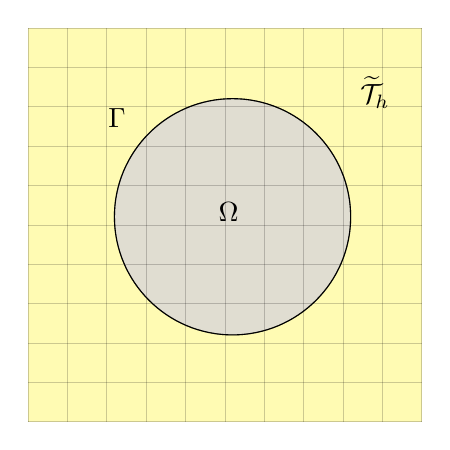
\begin{tikzpicture}[scale=1.0]

            \fill[yellow!30] (-2.5,2.5) -- (2.5,2.5) -- (2.5,-2.5) -- (-2.5,-2.5) -- cycle;
            \draw[fill=blue!30, opacity=0.4] (0.1, 0.1) circle (1.5cm);

            \draw (0.1, 0.1) circle (1.5cm);
            % Background mesh
            \foreach \i in {-2.5, -2, ..., 2.5} {
                \draw[line width=0.1pt, shift={(-2.5,\i)}, opacity=0.2] (0,0) -- (5,0);
                \draw[line width=0.1pt, shift={(\i,-2.5)}, opacity=0.2] (0,0) -- (0,5);
            }

            \node[below right] at (-0.2,0.4) {$\Omega$};
            \node[below right] at (-1.6,1.6) {$\Gamma$};

            % Labels
            \node[below right] at (1.6,2.0) {$\widetilde{\mathcal{T}}_{h}$};
        \end{tikzpicture}

}\hfill
\subfloat[]{\label{c}
        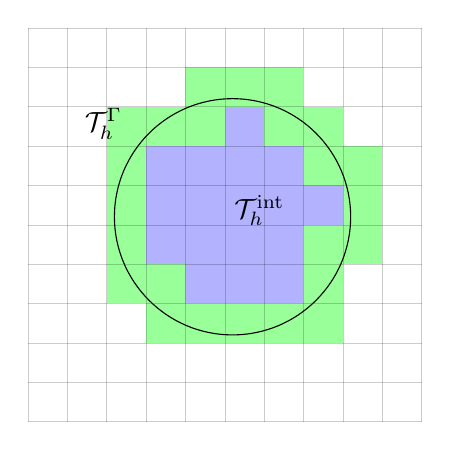
\begin{tikzpicture}[scale=1.0]

            % POTENTIAL ACTIVE MESH
            \fill[blue!30] (2,2) -- (2,-1.5) --(-1.5,-1.5) -- (-1.5,2) -- cycle;

            % ELEMENTS WITH NO INTERSECTION
            % lower left
            \fill[white] (-1.5,-1.5) rectangle (-1.0,-1.0);
            \fill[white] (-1.5,2.0) rectangle (-1.0,1.5);
            \fill[white] (-1.0,2.0) rectangle (-0.5,1.5);
            \fill[white] (2,2) rectangle (1.5,1.5);
            \fill[white] (1.5,2) rectangle (1.0,1.5);
            \fill[white] (2,1.5) rectangle (1.5,1.0);
            \fill[white] (1.5,-1) rectangle (2,-1.5);
            \fill[white] (1.5,-0.5) rectangle (2,-1.0);

            % CUT ELEMENTS
            \fill[green!40] (-0.5,2.0) rectangle (1.0,1.5);
            \fill[green!40] (-1.5,1.5) rectangle (0.0,1.0);
            \fill[green!40] (0.5,1.5) rectangle (1.5,1.0);
            \fill[green!40] (-1.5,1.0) rectangle (-1.0,-1.0);
            \fill[green!40] (-1.0,-0.5) rectangle (-0.5,-1.5);
            \fill[green!40] (-0.5,-1.5) rectangle (1.5,-1.0);
            \fill[green!40] (1.5,-1) rectangle (1.0,-0.0);
            \fill[green!40] (1.5,-0.5) rectangle (2.0,1.0);
            \fill[green!40] (1.0,0.5) rectangle (1.5,1.0);

            \draw (0.1, 0.1) circle (1.5cm);
            % Background mesh
            \foreach \i in {-2.5, -2, ..., 2.5} {
                \draw[line width=0.1pt, shift={(-2.5,\i)}, opacity=0.2] (0,0) -- (5,0);
                \draw[line width=0.1pt, shift={(\i,-2.5)}, opacity=0.2] (0,0) -- (0,5);
            }


            % Labels
            \node[below right] at (0.0,0.5) {$\mathcal{T}^{\mathrm{int} }_{h}$};
            \node[below right] at (-1.9,1.6) {$\mathcal{T}^{\Gamma }_{h}$};
        \end{tikzpicture}
}
\hfill
\subfloat[]{\label{b}
        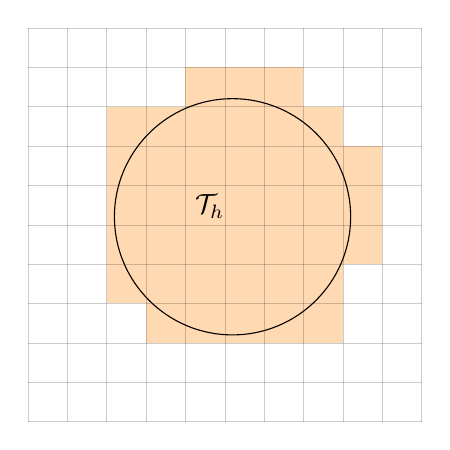
\begin{tikzpicture}[scale=1.0]

            % POTENTIAL ACTIVE MESH
            \fill[orange!30] (2,2) -- (2,-1.5) --(-1.5,-1.5) -- (-1.5,2) -- cycle;

            % ELEMENTS WITH NO INTERSECTION
            % lower left
            \fill[white] (-1.5,-1.5) rectangle (-1.0,-1.0);
            \fill[white] (-1.5,2.0) rectangle (-1.0,1.5);
            \fill[white] (-1.0,2.0) rectangle (-0.5,1.5);
            \fill[white] (2,2) rectangle (1.5,1.5);
            \fill[white] (1.5,2) rectangle (1.0,1.5);
            \fill[white] (2,1.5) rectangle (1.5,1.0);
            \fill[white] (1.5,-1) rectangle (2,-1.5);
            \fill[white] (1.5,-0.5) rectangle (2,-1.0);

            % CUT ELEMENTS
            \fill[orange!30] (-0.5,2.0) rectangle (1.0,1.5);
            \fill[orange!30] (-1.5,1.5) rectangle (0.0,1.0);
            \fill[orange!30] (0.5,1.5) rectangle (1.5,1.0);
            \fill[orange!30] (-1.5,1.0) rectangle (-1.0,-1.0);
            \fill[orange!30] (-1.0,-0.5) rectangle (-0.5,-1.5);
            \fill[orange!30] (-0.5,-1.5) rectangle (1.5,-1.0);
            \fill[orange!30] (1.5,-1) rectangle (1.0,-0.0);
            \fill[orange!30] (1.5,-0.5) rectangle (2.0,1.0);
            \fill[orange!30] (1.0,0.5) rectangle (1.5,1.0);

            \draw (0.1, 0.1) circle (1.5cm);
            % Background mesh
            \foreach \i in {-2.5, -2, ..., 2.5} {
                \draw[line width=0.1pt, shift={(-2.5,\i)}, opacity=0.2] (0,0) -- (5,0);
                \draw[line width=0.1pt, shift={(\i,-2.5)}, opacity=0.2] (0,0) -- (0,5);
            }


            % Labels
            % \node[below right] at (2.5,2.5) {$\widetilde{\mathcal{T}}_{h}$};
            % \node[below right] at (0.4,0.5) {$\mathcal{T}_{int}$};
            \node[below right] at (-0.5,0.5) {$\mathcal{T}_{h }$};
        \end{tikzpicture}


}


\caption{Illustration of the domain $\Omega$ with the corresponding boundary $\Gamma$, the background mesh $\widetilde{\mathcal{T}}_{h} $,  the cut cells $\mathcal{T} _{\Gamma }$, the interior cells $\mathcal{T} _{int}$ and the active set $\mathcal{T} _{h} =
\mathcal{T}^{ \mathrm{int}  }_{h} \cup \mathcal{T}_{h }^{ \Gamma  }  $. }
\label{fig:background_mesh}
\end{figure}


We want to devise a CutFEM based on the CIP formulation for the biharmonic problem. Assume that the physical domain $\Omega \subseteq    \mathbb{R} ^d$ to be open and bounded with a corresponding a sufficiently smooth boundary $\Gamma  $.
 Let $\widetilde{\mathcal{T}_{h} } $ be a shape-regular and quasi-uniform mesh which covers $\Omega $, but does not need to fit the
domain. Let us denote the active set $\mathcal{T} _{h} \subseteq \widetilde{\mathcal{T}_{h}}$ which intersects the interior of the active domain $\Omega $, that is
\begin{equation}
\label{eq:active_set}
\mathcal{T} _{h} = \left\{ T \in \widetilde{\mathcal{T} }_{h}  \mid  T \cap \Omega   \neq \emptyset    \right\}.
\end{equation}
We define the corresponding set of interior facets, \[
    \mathcal{F} _{h}^{\mathrm{int} } = \left\{ F = T^{+} \cap T^{-}  \mid  T^{+}, T^{-} \in \mathcal{T} _{h} \text{ and } T^{+} \neq T^{-} \right\},
\]
and the set of elements cut by the boundary \[
\mathcal{T}_{h} ^{\Gamma } = \left\{ T \in \mathcal{T} _{h}   \mid  T \cap \Gamma \neq \emptyset  \right\}.
\]
For convenience, will we define also the interior of the active set as $\mathcal{T} _{int}$.
\[
\mathcal{T} ^{\mathrm{int} }_{h} = \left\{ T \in \mathcal{T} _{h}   \mid  T \cap  \mathrm{Int}(\Omega ) \neq \emptyset  \right\}.
\]
Hence, we have that the active set is the union of the interior and cut elements, $\mathcal{T} _{h} = \mathcal{T}_{h} ^{\mathrm{int} } \cup  \mathcal{T} ^{\Gamma }_{h}$. For an illustration, see Figure \ref{fig:background_mesh}.



\subsection{Cut continuous interior penalty methods }%
\label{sub:cut_cip_method}

As $\Omega $ is static is it easy to observe that having a polynomial basis on the full mesh, $\widetilde{\mathcal{T}}_{h}$, is not necessary. Restricting us to the active set, we define the domain $\Omega _{h} = \bigcup _{T \in \mathcal{T} _{h}} T$.
Hence, we define the polynomial space only on the active set $\mathcal{T}_{h} $ from \eqref{eq:active_set},
\begin{equation}
V_{h} = \left\{ v \in C^{0}( \Omega _{h}  )  \mid  v_{T} = v | _{T} \in \mathcal{P} ^{k}\left( T \right) \text{ or } Q^{k}\left( T \right) \ \ \forall T \in
\mathcal{T}_{h}    \right\}.
\end{equation}
Here is $k$ the polynomial order.
Furthermore, drawing on the principles outlined in Section \ref{sec:CIP_biharmonic_problem}, we can indeed recall two CIP formulations for the biharmonic equation: the Hessian formulation \eqref{eq:hessian_prob} and the Laplace formulation \eqref{eq:laplace_prob}.

To make sure the problem is stabilized will we add a consistent symmetric positive semi-definite bilinear ghost-penalty term  $g_{h}: V_{h} \times  V_{h} \to \mathbb{R} $ to our bilinear form. That is, we define the discrete problem to be:
\begin{equation}
\label{eq:discrete_CutCIP_prob}
\text{ Find } u_{h} \in V_{h}  \text{ such that }    A_{h}( u_{h} ,v ) := a_{h}( u_{h}, v)  + g_{h}( u_{h},v) = l_{h} ( v) \quad  \forall v \in  V_{h}.
\end{equation}
Here $a_{h}( \cdot,\cdot  ) $ stand for either $a_{h}^{L}( \cdot ,\cdot ) $ or $a_{h}^{H}( \cdot ,\cdot ) $.

In this section, we provide a full proof for the Hessian formulation, however, the proof of the Laplace formulation does not differ too much. For simplification will we use the notation $a_{h}(u,v ) = a_{h}^{H}( u,v)$ and $l_{h}(v) =l_{h}^{H}(v)$ for the rest of the stability and convergence analysis.

Keep in mind that in contrast to the standard CIP methods our proposed method is defined on an unfitted mesh. As we will see in the analysis, the ghost penalty is a method to ensure numerical stability on cut cell $\mathcal{T} ^{\Gamma }_{h}$. The main reason why
this numerical instability is happening for a unfitted mesh is when a cell is badly cut, see examples in Figure \ref{fig:intersection-example}.
In other words, when a cell is "badly cut," it means that it is intersected by the boundary $\Gamma$ in such a way that only a very small part of the interior of an element $T$  intersects with the physical domain $\Omega $ , i.e. $\abs{ \Omega \cap
T }_{d} \ll h^{d}$. This can lead to both stability issues and a very poor condition number of the system matrix causing numerical instability.

The ghost penalty stabilization technique is designed to tackle this issue. Essentially, this approach introduces additional terms into the finite element method that penalize jumps in the discrete solution and its gradients across cell interfaces,
typically the cut-cells. This penalty not only improves the conditioning of the system matrix but also enhances the robustness of the method with respect to the location of the boundary inside each cell. However, to make this possible, we assume a
so-called fat-intersection property, which will be relevant in Section \ref{sec:constructing_ghost_penalties}.

Our first assumption as as follows;
for a $T \in \mathcal{T} ^{\Gamma }_{h}$ there always exists a patch $\omega ( T) $ which contains $T$ and an element $T'$ with a so-called fat intersection $
        \abs{ T' \cap \Omega  } _{d} \gtrsim \abs{ T' } _{d}$, where $\abs{ \cdot  }_{d} $ is the measure of an element of dimensions $d =2,3  $ . For an illustration, see Figure \ref{fig:fat_intersection_property}.

\begin{figure}[t]
    \centering
    \begin{tikzpicture}
        \coordinate (center) at (0, 0);

        % Reference hexagon vertices
        \coordinate (A1) at (0:2.5);
        \coordinate (A2) at (55:2.5);
        \coordinate (A3) at (125:2.5);
        \coordinate (A4) at (180:2.5);
        \coordinate (A5) at (235:2.5);
        \coordinate (A6) at (305:2.5);

        \fill[green!40] (center) --(A1) -- (A2) -- (A3) -- (A4) -- (A5)  -- cycle;
        \fill[blue!30] (center) -- (A5)--(A6) -- (A1) -- cycle;

        % Draw the individual edges
        \draw (center) -- (A1);
        \draw (center) -- (A2) --(A1);
        \draw (center) -- (A3);
        \draw (center) -- (A4);
        \draw (A2) -- (A3);
        \draw (A3) -- (A4);
        \draw (A5) -- (A6);
        \draw (A4) -- (A5);
        \draw (center) -- (A5);
        \draw (center) -- (A6) -- (A1);

        \coordinate (Ti) at (-0,-1.5);
        \coordinate (Tg) at (0.5,2.1);
        % \node[below] at (Tg) {$\mathcal{T}_{\Gamma }$};
        % \node[below] at (Ti) {$\mathcal{T}_{int }$};

        \coordinate (T0) at (1.1,1.0);
        \coordinate (T1) at (-1.1,-0.4);
        \node[below] at (T0) {$T$};
        \node[below] at (T1) {$T'$};

        \coordinate (C1) at (-3,-1.0);
        \coordinate (C2) at (2.6,0.4);
        \draw[-, line width=2pt, >=stealth] ($(C2)$) to[bend right=16.9] node[midway,xshift=-2.3cm, yshift=-1.3cm] {$\Gamma $} ($(C1)$);

        % \coordinate (D1) at (1,0.0);
        % \coordinate (D2) at (1.0,0.4);
        % \coordinate (D3) at (1.2,0.2);
        % \node at (D3) {$\varepsilon$};
        % \draw[line width=1.3pt, dotted] (D1) -- (D2);

        % Draw the line with brackets

    % Legend
    \begin{scope}[shift={(2.3,0.3)}]
        \draw (0,0.4) rectangle (1.3,1.5);
        \fill[green!30] (0.2,1.3) rectangle (0.4,1.1);
        \node[right] at (0.4,1.2) {$\mathcal{T}_{\Gamma}$};
        \fill[blue!30] (0.2,0.8) rectangle (0.4,0.6);
        \node[right] at (0.4,0.7) {$\mathcal{T}_{int}$};
    \end{scope}

    \end{tikzpicture}
\caption{Illustration of the fat intersection property. Let $T \in \mathcal{T}_{\Gamma } $. It shows a patch $\omega ( T) $ that contains elements $T \in  \mathcal{T}_{\Gamma } $ and $T'\in \mathcal{T} _{int} \cup \mathcal{T} _{\Gamma } = \mathcal{T} _{h}$, with $T' $ having a sufficiently large intersection with $\Omega$.}
    \label{fig:fat_intersection_property}
\end{figure}


We define the underlying norms for $ v \in V_{h} $ as
    \begin{align}
        \label{eq:bi_ah_norm}
        \| v \|_{ a_{h} }^{ 2 } & =    \alpha \|   v \|_{ \mathcal{T} _{h} \cap \Omega  }^{ 2}  + \| D^2 v \|_{\mathcal{T} _{h} \cap \Omega   }^{ 2 } +  \| h^{-\frac{1}{2}} \jump{ \partial _{n} v }   \|_{ \mathcal{F}_{h}^{}\cap \Omega    }^{ 2
        } +  \| h^{-\frac{1}{2}}  \partial _{n} v    \|_{ \Gamma   }^{ 2 },    \\
        \label{eq:bi_gh_norm}
\abs{ v } _{g_{h}}^{2} & = g( v,v), \\
        \label{eq:bi_Ah_norm}
\| v \|_{A_{h}  }^{  2}  & = \| v \|_{ a_{h} }^{ 2 } + \abs{ v } _{g_{h}}^{2}, \\
    \end{align}
and for $v \in V \oplus V_{h}$ we also introduce,
\begin{equation}
    \label{eq:astarnorm}
\| v \|_{ a_{h}, * }^{  2}  =\| v \|_{ a_{h} }^{ 2 } +  \| h^{\frac{1}{2}} \mean{ \partial _{nn} v }   \|_{\mathcal{F} _{h}^{} \cap \Omega   }^{  2} +  \| h^{\frac{1}{2}} \partial _{nn} v    \|_{ \Gamma }^{  2}.
\end{equation}
\begin{remark}
Note that it holds that $\mathcal{T} _{h} \cap  \Omega   = \Omega  $ and $\mathcal{T} _{h} \cap  \Gamma  = \Gamma $. Depending on context, we choose the best suitable notation.
\end{remark}
\begin{remark}
    The necessity to define the supplementary terms in the $\| \cdot   \|_{a{h},* }^{ } $  may raise certain questions.  The reason is because when $v$ is continuous, i.e. $v \in V$, the local inverse estimates  \ref{eq:fund_inv_est} does not hold for $\| \mean{ \partial
    _{nn} v }  \|_{ \mathcal{F}_{h} \cap \Omega    }^{  }  $ and  $\|  \partial
    _{nn} v   \|_{ \Gamma }^{  }  $ when evaluating $a_{h}( v, v) $. Hence, this leads necessity adding the additional terms into the norm.
\end{remark}


\subsection{Stability estimate}%
\label{sub:stability_estimate}


\begin{figure}[b]
    \centering
    \begin{minipage}{0.4\textwidth}
        \centering
        \begin{tikzpicture}
            \coordinate (center) at (0, 0);

            % Reference hexagon vertices
            \coordinate (A1) at (0:2.5);
            \coordinate (A2) at (55:2.5);
            \coordinate (A3) at (125:2.5);
            \coordinate (A4) at (180:2.5);
            \coordinate (A5) at (235:2.5);
            \coordinate (A6) at (305:2.5);

            \fill[green!40] (center) --(A1) -- (A2) -- (A3) -- (A4) -- (A5)  -- cycle;
            \fill[blue!30] (center) -- (A5)--(A6) -- (A1) -- cycle;

            % Draw the individual edges
            \draw (center) -- (A1);
            \draw (center) -- (A2) --(A1);
            \draw (center) -- (A3);
            \draw (center) -- (A4);
            \draw (A2) -- (A3);
            \draw (A3) -- (A4);
            \draw (A5) -- (A6);
            \draw (A4) -- (A5);
            \draw (center) -- (A5);
            \draw (center) -- (A6) -- (A1);

            \coordinate (Ti) at (-0,-1.5);
            \coordinate (Tg) at (0.5,2.1);
            % \node[below] at (Tg) {$\mathcal{T}_{\Gamma }$};
            % \node[below] at (Ti) {$\mathcal{T}_{int }$};

            \coordinate (T0) at (1.1,1.0);
            \coordinate (T1) at (-1.1,-0.4);
            \node[below] at (T0) {$T$};
            % \node[below] at (T1) {$T'$};

            \coordinate (C1) at (-3,-1.0);
            \coordinate (C2) at (2.6,0.4);
            \draw[-, line width=2pt, >=stealth] ($(C2)$) to[bend right=16.9] node[midway,xshift=-2.3cm, yshift=-1.3cm] {$\Gamma $} ($(C1)$);

            \coordinate (D1) at (1,0.0);
            \coordinate (D2) at (1.0,0.4);
            \coordinate (D3) at (1.2,0.2);
            \node at (D3) {$\varepsilon$};
            \draw[line width=1.3pt, dotted] (D1) -- (D2);

            % Draw the line with brackets

            % Legend
            % \begin{scope}[shift={(2.3,0.3)}]
            %     \draw (0,0.4) rectangle (1.3,1.5);
            %     \fill[green!30] (0.2,1.3) rectangle (0.4,1.1);
            %     \node[right] at (0.4,1.2) {$\mathcal{T}_{\Gamma}$};
            %     \fill[blue!30] (0.2,0.8) rectangle (0.4,0.6);
            %     \node[right] at (0.4,0.7) {$\mathcal{T}_{int}$};
            % \end{scope}

        \end{tikzpicture}
    \end{minipage}
    \hspace{1cm}
    \begin{minipage}{0.4\textwidth}
        \centering
        \begin{tikzpicture}
            \coordinate (center) at (0, 0);

            % Reference hexagon vertices
            \coordinate (A1) at (0:2.5);
            \coordinate (A2) at (60:2.5);
            \coordinate (A3) at (120:2.5);
            \coordinate (A4) at (180:2.5);
            \coordinate (A5) at (240:2.5);
            \coordinate (A6) at (300:2.5);
            \coordinate (A7) at (300:2.5);


            \fill[green!40] (center) --(A1) -- (A2) -- (A3) -- (A4) -- cycle;
            \fill[blue!30] (center) (A4) -- (A5)--(A6)-- (A7) -- (A1) -- cycle;

            % Draw the individual edges
            \draw (center) -- (A1);
            \draw (center) -- (A2) --(A1);
            \draw (center) -- (A3);
            \draw (center) -- (A4);
            \draw (A2) -- (A3);
            \draw (A3) -- (A4);
            \draw (A5) -- (A6);
            \draw (A4) -- (A5);
            \draw (center) -- (A5);
            \draw (center) -- (A6) -- (A1);

            \coordinate (Ti) at (-0,-1.5);
            \coordinate (Tg) at (0.5,2.2);
            % \node[below] at (Tg) {$\mathcal{T}_{\Gamma }$};
            % \node[below] at (Ti) {$\mathcal{T}_{int }$};

            \coordinate (T0) at (-0,1.9);
            \coordinate (T1) at (-1.1,-0.4);
            \node[below] at (T0) {$T$};

            \coordinate (C1) at (-3,0.7);
            \coordinate (C2) at (2.6,0.7);
            \draw[-, line width=2pt, >=stealth] ($(C2)$) to[bend right=0.9] node[midway,xshift=-2.5cm, yshift=-0.5cm] {$\Gamma $} ($(C1)$);
            % Legend
            \begin{scope}[shift={(2.3,0.4)}]
                \draw (0,0.4) rectangle (1.3,1.5);
                \fill[green!30] (0.2,1.3) rectangle (0.4,1.1);
                \node[right] at (0.4,1.2) {$\mathcal{T}^{\Gamma}_{h}$};
                \fill[blue!30] (0.2,0.8) rectangle (0.4,0.6);
                \node[right] at (0.4,0.7) {$\mathcal{T}^{\mathrm{int} }_{h}$};
            \end{scope}

            \coordinate (D1) at (0,0.0);
            \coordinate (D2) at (0.0,0.7);
            \coordinate (D3) at (0.3,0.2);
            \node at (D3) {$\varepsilon$};
            \draw[line width=1.3pt, dotted] (D1) -- (D2);

        \end{tikzpicture}
    \end{minipage}
        \caption{Illustration of two examples of bad cut cells with an arbitrary small length $\varepsilon \ll 1 $. Let $T \in  \mathcal{T}^{\Gamma }_h $ be a cut cell.  On the left example, is it clear that $\abs{ \Gamma \cap T }
            \lesssim  h^{d-1}$ and $  \ \abs{ \Omega  \cap T } \lesssim  \varepsilon  h^{d}$  . However, on the right example is it clear that  $\abs{ \Gamma \cap T }
            \lesssim  \varepsilon h^{d-1}$ and $\abs{ \Omega  \cap T } \lesssim  \varepsilon  h^{d}$.}
        \label{fig:intersection-example}
\end{figure}

% From basic theory we have the following inverse estimate for $ v \in \mathcal{P}^{k}( T)$ s.t. \[
%      \| \partial _{nn}  v \|_{F   }^{ }  \lesssim  \| h_{T}^{-\frac{1}{2}} D ^2 v \|_{ T }^{  },
% \]
% where the hidden constant depend on dimension $d$, order $k$ and the shape regularity.

Recall the Subsection \ref{sub:some_general_inequalities} where we discussed standard local inverse estimates.
Similarly for cut elements is it easy to see that this must hold,
\begin{equation}
     \| \partial _{nn}  v_{h} \|_{F \cap \Omega    }^{  }  \lesssim\| \partial _{nn}  v_{h} \|_{F }^{  }  \lesssim   \| h_{T}^{-\frac{1}{2}} D ^2 v_{h} \|_{ T }^{  }.
\end{equation}
A useful variant is the following inequality that is,
\begin{equation}
    \label{eq:inv_full}
\| \partial _{nn} v_{h} \|_{ \Gamma \cap T  }^{  } \lesssim h^{-\frac{1}{2}} \| D^2 v_{h} \|_{ T }^{  }.
\end{equation}
\begin{remark}
    It may be natural to instead look at $\| \partial _{nn} v_{h} \|_{ \Gamma \cap T  }^{  } \lesssim h^{-\frac{1}{2}} \| D^2 v_{h} \|_{ T\cap \Omega  }^{  }$, however, this cannot hold for a arbitary cut configutration for an unfitted mesh. To demonstrate, let $\varepsilon \ll 1$ be a small length. For the examples provided in
    Figure \ref{fig:intersection-example} we have two cases: i) $\abs{ \Gamma \cap \Omega  }_{d-1} \lesssim \varepsilon h^{d-1}  $ and $\abs{ T \cap \Omega  }_{d-1} \lesssim \varepsilon h^{d-1}  $, and ii)
    $\abs{ \Gamma \cap \Omega  }_{d-1} \lesssim  h^{d-1}  $ and $\abs{ T \cap \Omega  }_{d-1} \lesssim \varepsilon h^{d-1}  $.
    The first first case impacts the condition number since it is introducing almost vanishing entries in the system matrix from \eqref{eq:linear_system}.
    While for the second case is bad for inverse estimates, and, thus, problematic for proving coercivity. To recover, one in fact must incorporate the full element $T$ into the inverse estimate.
\end{remark}


Since the inequalities above holds for all elements locally is it natural to extend it to the full mesh  $\mathcal{T}_{h} $. This implies that
\begin{align}
\label{eq:bi_cut_inverse_1}
\| \partial _{nn} v_h \|_{ \mathcal{T} _{h} \cap \Gamma  }^{  } &\lesssim h^{-\frac{1}{2}} \| D^2 v_h \|_{ \mathcal{T}_h }^{  }, \\
\label{eq:bi_cut_inverse_2}
\| \partial _{nn}  v_h \|_{ \mathcal{F}_h \cap \Omega    }^{  }  &  \lesssim   h^{-\frac{1}{2}} \| D^2 v_h \|_{ \mathcal{T}_h  }^{  }.
\end{align}
    We aware that these inequalities also holds for the first order, that is.
\begin{align}
\label{eq:bi_n_cut_inverse_1}
\| \partial _{n} v_h \|_{ \mathcal{T} _{h} \cap \Gamma  }^{  } &\lesssim h^{-\frac{1}{2}} \| \nabla v \|_{ \mathcal{T}_h }^{  }, \\
\label{eq:bi_n_cut_inverse_2}
\| \partial _{n}  v_h \|_{ \mathcal{F}_h \cap \Omega    }^{  }  &  \lesssim   h^{-\frac{1}{2}} \| \nabla v_h \|_{ \mathcal{T}_h  }^{  }.
\end{align}
In fact, combining the second order inequalities we get the following identity.
\begin{equation}
\label{eq:bi_identity}
h\| \partial _{nn}  v_{h} \|_{ \mathcal{F}_h \cap \Omega    }^{2 } + h\| \partial _{nn} v_{h} \|_{ \mathcal{T} _{h} \cap \Gamma  }^{2  } \lesssim \| D^2 v_{h} \|_{ \mathcal{T} _{h}  }^{2  } \quad  \forall v_{h} \in V_{h}.
\end{equation}
For more information about the derivations of the inequalities, see discussion in \cite[Section 2.4]{gurkan2019stabilized}.

We may introduce our first assumption on the ghost penalty.  Inspired by the expansion for the $H^{1}$-norm as detailed in \cite[Equation 2.23]{gurkan2019stabilized}, we adopt an analogous approach for the $H^{2}$-norm in this scenario.
\begin{assumption*}[EP1]
    \label{as:bi_EP1}
    The ghost penalty $g_{h}$ extends the $H^{2}$ norm such that
    \begin{equation*}
    \| D^2 v \|_{ \mathcal{T} _{h} }^{ 2 } \lesssim  \| D^2 v \|_{ \Omega  }^{ 2 } + \abs{ v } _{g_{h}}^{2}.
    \end{equation*}
\end{assumption*}


Combing the results we get the following convenient corollary.

\begin{corollary}
    \label{cor:bi_inverse_thm}
    Let  $g_{h}$ satisfy Assumption \ref{as:bi_EP1}, then
    \begin{equation}
        \label{eq:inv_est}
            h\| \partial _{nn}  v_{h} \|_{ \mathcal{F}_h^{} \cap \Omega    }^{2 } + h\| \partial _{nn} v_{h} \|_{ \mathcal{T} _{h} \cap \Gamma  }^{2  }   \lesssim  \| D^2 v_{h} \|_{ \Omega  }^{ 2 } + \abs{ v_{h} } _{g_{h}}^{2} \\
              \lesssim \| v_{h} \|_{ A_{h} }^{  2} \quad  \forall v_{h} \in V_{h}
    \end{equation}
    From this is it also clear that \begin{equation}
        \label{eq:asta_Ah}
    \| v_{h} \|_{ a_{h},* }^{  }  \lesssim \| v_{h} \|_{ A_{h} }^{  } \quad  \forall v_{h} \in V_{h}
    \end{equation}
\end{corollary}
\begin{proof}
    The the first result \eqref{eq:inv_est} is a direct result of \eqref{eq:bi_identity}, Assumption \ref{as:bi_EP1} and the definition of $\| \cdot  \|_{ A_{h} }^{  } $.
    The second result \eqref{eq:asta_Ah} is simply a observation that the terms in \eqref{eq:inv_est} appears in $\| \cdot   \|_{a_{h},*  }^{  } $, hence, the inequality follows.
\end{proof}

\begin{lemma}
    \label{lemma:bi_Ah_coercive}
    The discrete form $A_{h}$ is coercive, that is, \[
    \| v_{h} \|_{ A_{h} }^{ 2 }  \lesssim A_{h}( v_{h},v_{h})\quad  \forall v_{h} \in V_{h}.
    \]
\end{lemma}

\begin{proof}
    Let $v_{h} \in V_{h}$.
    Observe that
    \begin{equation}
    A_{h}( v_{h},v_{h}) = a_{h}( v_{h},v_{h})  + \abs{ v_{h} }_{g_{h}}^{2}
    \end{equation}
    Firstly, the ghost penalty term is already a part of the $\| \cdot  \|_{ A_{h} }^{  } $ norm, hence, it only remains to check the $a_{h}( \cdot ,\cdot ) $ term.
    \begin{equation}
        \label{eq:coerciv_ah}
    \begin{split}
       a_{h}( v_{h},v_{h}) &=   \alpha \| v_{h} \|_{   \Omega   }^{2} + \| D^2v_{h} \|_{   \Omega  }^{2  }  + \frac{\gamma }{h}  \|  \jump{ \partial _{n} v_{h} }\|_{\mathcal{F} _{h}^{}  }^{ 2 } + \frac{\gamma }{h}  \| \partial _{n} v_{h} \|_{ \Gamma  }^{ 2 }. \\
                   & + 2 ( \mean{ \partial _{nn} v_{h} }, \jump{ \partial _{n} v_{h} }    )_{\mathcal{F} ^{}_{h} \cap \Omega }  + 2 (  \partial _{nn} v ,
       \partial _{n} v_{h}  )_{\Gamma } \\
    \end{split}
    \end{equation}
    We first focus on the last two terms in \eqref{eq:coerciv_ah}. Using Cauchy-Schwarz \eqref{eq:cauchy-schwartz}, we observe that
    \begin{equation}
        \begin{split}
    ( \mean{ \partial _{nn} v_{h} }  , \jump{ \partial _{n} v_{h} }  )_{\mathcal{F}^{}_{h}\cap \Omega  } & \ge - \| h^{\frac{1}{2}}\mean{ \partial _{nn} v_{h} }   \|_{ \mathcal{F}^{}_{h}\cap \Omega   }^{  }  \|h^{-\frac{1}{2}} \jump{ \partial _{n} v_{h} }   \|_{
    \mathcal{F}^{}_{h}\cap \Omega   }^{  } \\
    (  \partial _{nn} v_{h}   ,  \partial _{n} v_{h}   )_{\Gamma   } & \ge - \| h^{\frac{1}{2}} \partial _{nn} v_{h}    \|_{ \Gamma    }^{  }  \|h^{-\frac{1}{2}}  \partial _{n} v_{h}    \|_{ \Gamma    }^{  }
        \end{split}
    \end{equation}
    Using inverse-inequalities \eqref{eq:bi_cut_inverse_1} and \eqref{eq:bi_cut_inverse_2} and the Corollary \ref{cor:bi_inverse_thm} can we easily observe that
    \begin{equation}
        \begin{split}
     \| h^{\frac{1}{2}} \mean{ \partial _{nn}v_{h} } \|_{ \mathcal{F}_{h} \cap \Omega    }^{  2} & \le C_{1} \| D^2 v_{h} \|_{ \mathcal{T}_{h}   }^{2  } \lesssim   \| D^2 v_{h} \|_{ \Omega  }^{ 2 }  + \abs{ v_{h} } _{ g_{h} }^{2  }   \\
     \|  \partial _{nn}v_{h}  \|_{ \Gamma     }^{ 2 } & \le C_{2} \| D^2 v_{h} \|_{ \mathcal{T} _{h}  }^{2  } \lesssim    \| D^2 v_{h} \|_{ \Omega  }^{ 2 }  + \abs{ v_{h} } _{ g_{h} }^{2  }
        \end{split}
    \end{equation}
    Thus, by applying Youngs $\varepsilon $-inequality \eqref{eq:young-epsilon}, is it natural to see that,
    \begin{equation}
        \begin{split}
- C_{1}^{\frac{1}{2}} \| D^2 v_{h}    \|_{ \mathcal{T} _{h}   }^{  }  \|h^{-\frac{1}{2}} \jump{ \partial _{n} v_{h} }   \|_{ \mathcal{F}^{}_{h}\cap \Omega   }^{  }
& \ge - \frac{1}{\varepsilon } C  (\| D^2 v_{h} \|_{ \Omega  }^{ 2 }  + \abs{ v_{h} } _{ g_{h} }^{2  } ) -  \varepsilon \|h^{-\frac{1}{2}} \jump{ \partial _{n} v_{h} }   \|_{ \mathcal{F}^{}_{h}\cap \Omega   }^{2  } \\
- C_{2}^{\frac{1}{2}}  \| D^2 v_{h} \|_{ \mathcal{T} _{h} }^{  } \| h^{-\frac{1}{2}}  \partial _{n} v_{h}    \|_{ \Gamma    }^{  }
& \ge - \frac{1}{\varepsilon } C  (\| D^2 v_{h} \|_{ \Omega  }^{ 2 }  + \abs{ v_{h} } _{ g_{h} }^{2  } ) -  \varepsilon \|h^{-\frac{1}{2}}  \partial _{n} v_{h}    \|_{ \Gamma    }^{2  } \\
        \end{split}
    \end{equation}
    Combining these ideas do we end up with the following inequality,
    \begin{equation}
    \begin{split}
       a_{h}( v_{h},v_{h})  \ge& \  \alpha     \|\  v  \|_{   \Omega   }^{2} +\| D^2v_{h}  \|_{   \Omega   }^{2} -  \frac{1}{\varepsilon } 4C  (\| D^2 v_{h} \|_{ \Omega  }^{ 2 }  + \abs{ v_{h} } _{ g_{h} }^{2  } )  \\
                       & + (\gamma - 2\varepsilon  )\left( \|h^{-\frac{1}{2}}  \jump{ \partial _{n} v_{h} }\|_{\mathcal{F} _{h}^{} \cap \Omega   }^{ 2 } + \| h^{-\frac{1}{2}} \partial _{n} v_{h} \|_{ \Gamma  }^{ 2} \right)        \\
    \end{split}
    \end{equation}
    This inequality is useful since if we add a ghost penalty on the left hand side we get,
    \begin{equation}
        \begin{split}
     A_{h}( v_{h},v_{h}) & = a( v_{h},v_{h}) + \abs{ v_{h} }_{g_{h}}^{2} \\
     & \gtrsim    \   \| \ |\alpha|^{\frac{1}{2}} \  v_{h}  \|_{   \Omega   }^{2} + (1  - \frac{1}{\varepsilon } 4C)  (\| D^2 v_{h} \|_{ \Omega  }^{ 2 }  + \abs{ v_{h} } _{ g_{h} }^{2  } )  \\
                       & + (\gamma - 2\varepsilon  )\left( \|h^{-\frac{1}{2}}  \jump{ \partial _{n} v_{h} }\|_{\mathcal{F} _{h}^{}\cap \Omega   }^{ 2 } + \| h^{-\frac{1}{2}} \partial _{n} v_{h} \|_{ \Gamma  }^{ 2} \right)        .
        \end{split}
    \end{equation}
    Setting $\varepsilon = 8C$ and $\gamma = 32C $ we arrive at the desired state,
    \begin{equation}
        \begin{split}
           A_{h}( v_{h},v_{h})  \gtrsim & \   \| \ |\alpha|^{\frac{1}{2}} \    v_{h}  \|_{  \Omega   }^{2} + \frac{1}{2}  (\| D^2 v_{h} \|_{ \Omega  }^{ 2 }  + \abs{ v_{h} } _{ g_{h} }^{2  } )  \\
                       & + \frac{\gamma }{2}\left( \|h^{-\frac{1}{2}}  \jump{ \partial _{n} v_{h} }\|_{\mathcal{F} _{h}^{}\cap \Omega   }^{ 2 } + \| h^{-\frac{1}{2}} \partial _{n} v_{h} \|_{ \Gamma  }^{ 2} \right) \\
                        \gtrsim & \  \| v_{h} \|_{ A_{h} }^{2  }
        \end{split}
.
    \end{equation}
\end{proof}


\begin{lemma}
    \label{lemma:bi_Ah_bounded}
    The discrete form $A_{h}$ is bounded, that is,
    \begin{equation}
    \label{eq:bi_A_h_bounded}
     A_{h}( v_{h},w_{h}) \lesssim \| v_{h} \|_{A_{h}  }^{  }\| w_{h} \|_{A_{h}  }^{  } \quad   \forall v_{h},w_{h} \in V_{h}
    \end{equation}
    Moreover, for $v \in V_{h} \oplus V$  and $w_{h} \in V_{h}$ the discrete bilinear form $a_{h}( \cdot ,\cdot  ) $ satisfies,
    \begin{equation}
        \label{eq:bi_a_h_bounded}
        a_{h} ( v,w_{h}) \lesssim \| v \|_{ a_{h},* }^{  } \| w_{h} \|_{ A_{h} }^{  }.
    \end{equation}
\end{lemma}

\begin{proof}
         \textbf{Step 1.} The goal is to prove the inequality \eqref{eq:bi_A_h_bounded}.
         \begin{equation}
                \abs{ A_{h}( v_{h} ,w_{h} ) } \lesssim   \abs{a_{h}( v_{h}, w_{h}) }   + \abs{g_{h}( v_{h},w_{h})  }
         \end{equation}
                By assumption is the ghost penalty $g_{h}$ positive semi-definite, thus, it fulfills the Cauchy-Schwarz inequality \eqref{eq:cauchy-schwartz},
                \begin{equation}
                \abs{ g_{h}(v_{h},w_{h} ) } \lesssim \abs{ v_{h} } _{g_{h}}\abs{ w_{h} }_{g_{h}}.
                \end{equation}
                Hence, by definition of $A_{h}( \cdot ,\cdot ) $, is $\abs{ g_{h}(v_{h},w_{h} ) } \lesssim \| v_{h} \|_{ A_{h} }^{  } \| w_{h} \|_{ A_{h} }^{  } $. It remains to show that the bilinear term $ a_{h}( \cdot ,\cdot ) $ is bounded. We numerate the terms in this fashion.
                \begin{equation}
                    \begin{split}
                         a_{h} \left( v_{h}, w_{h} \right)    \le  &   \left( \alpha  v_{h}, w_{h} \right) _{\mathcal{T} _{h} \cap \Omega }      +  \left( D^2 v_{h}, D^2w_{h} \right) _{\mathcal{T} _{h} \cap \Omega}    \\
                                                     & + \left( \mean{  \partial _{n n} v_{h} }, \jump{ \partial _{n }w_{h}} \right)_{\mathcal{F}_{h}^{} \cap \Omega}     + \left( \mean{ \partial _{nn } w_{h} }, \jump{ \partial _{n}v_{h} }
                                                     \right)_{\mathcal{F}_{h}^{} \cap \Omega}+ \frac{\gamma }{h}  \left( \jump{ \partial _{n} v_{h}}, \jump{ \partial _{n} w_{h}   }   \right)_{\mathcal{F}_{h}^{} \cap \Omega}   \\
                                                     & + \left(  \partial _{n n} v_{h} ,  \partial _{n }w_{h} \right)_{\Gamma } + \left(  \partial _{n n} w_{h} ,  \partial _{n}v_{h}       \right)_{\Gamma }   + \frac{\gamma }{h}  \left(  \partial _{n}
                                                         v_{h},  \partial
                                                     _{n} w_{h} \right)_{\Gamma } \\
                                                     &=  ( \mathrm{I} ) + \ldots+( \mathrm{VIII} )     \\
                    \end{split}
                \end{equation}
                The strategy is to bound each term individually using Cauchy-Schwarz \eqref{eq:cauchy-schwartz}. From this is it easy to see that $\abs{( \mathrm{I} )   } +  \abs{( \mathrm{II} )   }   \lesssim \| v_{h} \|_{a_{h}  }^{  } \| w_{h} \|_{ a_{h}
                }^{  } $. For the terms symmetrical terms $(
                \mathrm{III} ) $ and  $( \mathrm{IV} ) $ we apply the inverse inequality
                \eqref{eq:bi_cut_inverse_2}.
                \begin{equation}
                    \label{eq:invest_1}
                    \abs{(\mathrm{III} )  }  \lesssim  \|h^{\frac{1}{2}} \partial _{n n} v_{h}  \|_{ \mathcal{F}_{h}^{} \cap \Omega}^{  }\| h^{-\frac{1}{2}} \jump{ \partial _{n} w_{h} }     \|_{\mathcal{F}_{h}^{} \cap \Omega}^{  } \lesssim  \| v_{h} \|_{A_{h}
                    }^{  } \|w    \|_{ a_{h}}^{  }.
                \end{equation}
                Here we used that  $\|h^{\frac{1}{2}} \partial _{n n}  v_{h} \|_{\mathcal{F}_{h}^{} \cap \Omega} \lesssim \| v_{h} \|_{ A_{h}  }^{  }  $ thanks to Corollary \ref{cor:bi_inverse_thm}.
              The interior penalty can we easily see that,
              \begin{equation}
              \abs{ ( \mathrm{V} )  }  \lesssim  \|h^{-\frac{1}{2}} \jump{ \partial _{n} v_{h}}  \|_{ \mathcal{F}_{h}^{} \cap \Omega }^{  }
             \|h^{-\frac{1}{2}} \jump{ \partial _{n} w_{h}}  \|_{ \mathcal{F}_{h}^{} \cap \Omega }^{  }  \lesssim  \| v_{h}  \|_{ a_{h} }^{  }
             \| w_{h}  \|_{ a_{h} }^{  }.
              \end{equation}
              It remains to handle the symmetry terms $ ( \mathrm{VI} )$ and $ ( \mathrm{VII} )$.
              \begin{equation}
                    \label{eq:invest_2}
                \abs{ ( \mathrm{VI} )  }  \lesssim \| h^{\frac{1}{2}}\partial _{nn} v_{h} \|_{\Gamma   }^{  } \| h^{-\frac{1}{2}} \partial _{n}w_{h} \|_{\Gamma   }^{  }  \lesssim \|  v_{h} \|_{A_{h}  }^{  } \| w_{h} \|_{ a_{h}   }^{  }
              \end{equation}
             Again, here we used the Corollary \ref{cor:bi_inverse_thm}.
             Finally, using the definition of the norm is it easily to see that,
             \[
\abs{ ( \mathrm{VIII} )  }  \lesssim \| \partial _{n}v_{h} \|_{ \Gamma  }^{  }
\| \partial _{n} w_{h} \|_{ \Gamma  }^{  }  \lesssim \| v_{h} \|_{ a_{h} }^{  }
\| w_{h} \|_{ a_{h} }^{  } .
             \]

             Hence, we can conclude \begin{equation}
                 \label{eq:ah_ahnorm}
                 \abs{ a_{h}( v_{h},w_{h})  } \le \| v_{h} \|_{ a_{h} }^{  } \| w_{h} \|_{ a_{h} }^{  } \forall v_{h},w_{h} \in V_{h}.
             \end{equation}
             Therefore, since $\| \cdot  \|_{a_{h}  }^{  } \lesssim  \| \cdot  \|_{A_{h}  }^{  } $, it has been demonstrated that $a_{h}( \cdot ,\cdot )$ is bounded within the $\|\cdot   \|_{A{h} }^{ }$ norm.

             \textbf{Step 2.} The goal is to prove \eqref{eq:bi_a_h_bounded}. Let $v \in V_{h} \oplus V $ and $w_{h} \in V_{h}$.
             The only difference is that since $v$ is continious we cannot apply to Corollary \ref{cor:bi_inverse_thm} on the estimates \eqref{eq:invest_1} and \eqref{eq:invest_2}. However, this is not a problem since $\| h^{\frac{1}{2}} \mean{ \partial _{nn} v }
             \|_{\mathcal{F} _{h}\cap  \Omega   }^{  } $ and  $\|h^{\frac{1}{2}}  \partial _{nn}v \|_{\Gamma   }^{  } $ are terms in the norm $\|  v \|_{a_{h},*  }^{  } $. Thus, we know that
             \begin{equation}
                  \abs{ a_{h}( v,w_{h}) }  \le \| v \|_{ a_{h},* }^{  } \| w_{h} \|_{ A_{h} }^{  } \ \ \forall v \in V_{h} \oplus V \text{ and } w_{h} \in V_{h}
             \end{equation}

\end{proof}





    % 
\subsection{A priori error estimate}%
\label{sec:a_priori_estimates}


For the proposed method, we want to derive a priori error estimate with respect to both the  $\| \cdot  \|_{a_{h},*   }^{  } $-norm and the  $\| \cdot  \|_{ \Omega  }^{
} $-norm.  These estimates are geometrically robust in that they remain unaffected by specific cut configurations, thanks to the ghost penalty they incorporate.
First, we construct a suitable (quasi-)interpolation operator, here we use the Clement quasi interpolation operator which in contrast to the standard Lagrange nodal interpolation operator is also defined for low regularity function $u \in L^{2}(
\Omega ) $.
In combination with discrete coercivity this allows us to derive an a priori error estimate in the energy norm. Finally, we use a standard duality argument, also known as Aubin-Nitsche trick, to derive the $L^{2}( \Omega ) $-error estimate.

Recall that for $v \in H^{3}( \mathcal{T } _{h}) $ the following inequalities.
\begin{align}
    \label{eq:trace:1}
    \| \nabla v \|_{ \partial T }^{  } &\lesssim h^{-\frac{1}{2}}_{T}\|  \nabla v \|_{ T }^{  }+ h^{\frac{1}{2}} \| D^2 v \|_{T  }^{   }  , \\
    \label{eq:trace:2}
    \| \nabla v \|_{ \Gamma \cap T }^{  } &\lesssim  h^{-\frac{1}{2}} \| \nabla v \|_{T  }^{  }   + h^{\frac{1}{2}}_{T} \| D^2 v \|_{ T }^{  },\\
    \label{eq:trace:3}
    \| D^2 v \|_{ \Gamma \cap T }^{  } &\lesssim  h^{-\frac{1}{2}} \| D^2 v \|_{T  }^{  }   + h^{\frac{1}{2}}_{T} \| D^3 v \|_{ T }^{  },
\end{align}
holds $\forall T \in \mathcal{T} _{h}$, for proof see \cite[Lemma 4.2]{hansbo2003finite}. In this context is $D^3v$ a tensor defined in Equation \eqref{eq:tensor}.

Assume that $\Omega $ has a boundary $\Gamma $ in $C^{1}$, then there exists a bounded extension operator,
\begin{equation}
    ( \cdot ) ^{e}: H^{m}( \Omega )  \to H^{m} ( \mathbb{R} ^{d}),
\end{equation}
for all  $v \in H^{m}( \Omega )$ which satisfies
\begin{equation}
    \begin{split}
 v^{e}| _{\Omega } =   v,  \\
\| v^{e} \|_{ m,\mathbb{R} ^{d}  }^{  } & \lesssim \| v \|_{ m, \Omega  }^{  }.
    \end{split}
\end{equation}
For more information, see \cite[Theorem 9.7]{brezis2011functional} and \cite[p.181, p.185]{stein1970singular}. For the notation we simply write $ v := v^{e}   $ for $v \in \mathbb{R} ^{d} \setminus \Omega $.


Starting from Lemma \ref{lemma:clements}, assume $v \in H^{s}( \Omega ) $ and let $r = \mathrm{min}(s , k+1) $. Revisit the definition of $V_{h}$ from \eqref{eq:vh_energy}, which is a polynomial of degree $k$. We can then employ the combination of the Clément interpolator with the extension operator to create $C_{h}^{e}: H^{m}( \mathbb{R} ^{d}) \to V_{h}$, such that $C ^{e} _{h} v := C _{h} v^{e}$.
 Next, recall that $ \sum_{T\in \mathcal{T}_{h}}^{} \| v \|_{s,\omega ( T)   }^{  } \le C  \| v \|_{s, \mathcal{T}_{h}   }^{  } $ where $C$ is some constant decided by shape regularity of the mesh and the maximal number of different patches a single element can
 belong to. This also holds for the inequality $ \sum_{T \in \mathcal{T}_{h} }^{} \sum_{F \in \partial T}^{}  \| v \|_{s,\omega ( F)   }^{  } \le C  \| v \|_{s, \mathcal{T}_{h}   }^{  } $.
The following estimates are thereby established.

\begin{align}
    \label{eq:bi_projection_estimates_1}
    \| v - C _{h}^{e} v \|_{  l, \mathcal{T} _{h} }^{  } & \lesssim h^{r-l}\sum_{T \in \mathcal{T}_h} \| v \|_{ r, \omega(T) }^{  } \lesssim  h^{r-l-\frac{1}{2}}  \| v \|_{ r, \Omega  }^{  }, \quad 0\le l\le r, \\
    \label{eq:bi_projection_estimates_2}
\| v - C ^{e}_{h}v \|_{ l, \partial \mathcal{T} _{h} }^{  } & \lesssim h^{r-l-\frac{1}{2}}\sum_{T \in \mathcal{T}_h} \sum_{F \in \partial T} \| v \|_{ r, \omega(F)  }^{  } \lesssim h^{r-l-\frac{1}{2}} \| v \|_{ r, \Omega   }^{  }, \quad 0  \le  l \le   r-\frac{1}{2}.
    % \label{eq:bi_projection_estimates_3}
    % \| v - C ^{e}_{h}v \|_{ l, \Gamma }^{  } & \lesssim h^{r-l-\frac{1}{2}} \sum_{T \in \mathcal{T}_h}  \| v \|_{ r,  \omega(T)  }^{  }\lesssim h^{r-l-\frac{1}{2}} \lesssim    \| v \|_{ r,  \Omega   }^{  }, \quad 0  \le  l \le  r-\frac{1}{2}.
\end{align}

% \todo[inline]{ Maybe hard to argue \eqref{eq:bi_projection_estimates_3} to hold on $\Gamma $, but may be related to some generalization of \eqref{eq:bi_n_cut_inverse_1} and \eqref{eq:bi_cut_inverse_1}. Anyhow, \eqref{eq:bi_projection_estimates_2} and
% \eqref{eq:bi_projection_estimates_3} was never used in the proof of Lemma \ref{lemma:astar_estimate} since we used inverse estimates and ended up with \eqref{eq:bi_projection_estimates_1} instead on all of them.}

\begin{lemma}
    \label{lemma:astar_estimate}
    Let $u \in H^{s}( \Omega ) $ for $s\ge 3$ be the exact solution to $\eqref{eq:cont_weak_problem} $ and let $k$ be the polynomial order of $V_{h}$. Set $r = \mathrm{min} ( s, k+1)$, then we have the interpolation estimates
    \begin{equation}
    \|  u - C_{h}u \|_{ a_{h},*  }^{  } \lesssim h^{r-2} \| u \|_{ r, \Omega  }^{  }.
    \end{equation}
\end{lemma}

\begin{proof}
    By definition,
    \begin{equation}
        \begin{split}
            \| u - C_{h}^{e}u \|_{ a_{h}, * }^{  2}  =& \ \alpha  \overbrace{\|  ( u - C_{h}^{e}u) \|_{ \mathcal{T} _{h} \cap \Omega  }^{ 2}}^{\mathrm{I} }   + \overbrace{\| D^2 ( u - C_{h}^{e}u ) \|_{\mathcal{T} _{h} \cap \Omega   }^{ 2
            }}^{\mathrm{II} }  \\  &  +
            \overbrace{\gamma \| h^{-\frac{1}{2}} \jump{ \partial _{n} (u -
        C_{h}^{e} u) }   \|_{ \mathcal{F}_{h}^{}\cap \Omega    }^{ 2
        }}^{\mathrm{III} }  + \overbrace{\gamma \| h^{-\frac{1}{2}}  \partial _{n} (u - C_{h}^{e}u)    \|_{ \Gamma   }^{ 2 }}^{\mathrm{IV} }  \\
          & + \overbrace{\| h^{\frac{1}{2}} \mean{ \partial _{nn} (u - C_{h}^{e}u) }   \|_{\mathcal{F} _{h}^{} \cap \Omega   }^{  2}}^{\mathrm{V} }  +  \overbrace{\| h^{\frac{1}{2}} \partial _{nn}(u - C_{h}^{e}u)     \|_{ \Gamma }^{  2}}^{\mathrm{VI}
          } \\
          =& \  \mathrm{I}  + \ldots + \mathrm{VI}.
        \end{split}
    \end{equation}
    The strategy is to bound each term individually.
    By initially focusing on the first two terms and employing equation \eqref{eq:bi_projection_estimates_1}, we can easily observe
             \begin{equation}
        \begin{split}
            \mathrm{I} +\mathrm{II}  & \lesssim \|   u - C_{h}^{e}u \|_{ \mathcal{T} _{h}  }^{ 2} + \|  D^2( u - C_{h}^{e}u )  \|_{\mathcal{T} _{h} }^{ 2 } \\
                                     & \lesssim  ( h^{2r}  + h^{2(r-2)} )\| u \|_{r,\mathcal{T}_{h} }^{  2} \lesssim h^{2(r -2)} \| u
                                     \|_{r, \mathcal{T} _{h} }^{2  }  .
        \end{split}
             \end{equation}
    From \eqref{eq:mean_jump_estimate} is it clear that $\| \jump{ \partial _{n} u }   \|_{ \mathcal{F}_{h}   }^{  } \lesssim \| \nabla  u \|_{ \partial  \mathcal{T} _{h} }^{  }   $. Hence, first applying the trace inequality \eqref{eq:trace:1}  and then
    \eqref{eq:bi_projection_estimates_1} is it clear that,
    \begin{equation}
        \begin{split}
            \mathrm{III}  & \lesssim h^{-1} \|  \nabla ( u - C_{h}^{e})  \|_{\partial \mathcal{T}_{h}   }^{2  }  \lesssim h^{-2} \| \nabla ( u - C^{e}_{h}u)  \|_{ \mathcal{T} _{h}
                          }^{ 2 } + \|  D^2  ( u - C_{h}^{e})  \|_{\mathcal{T}_{h}   }^{ 2 } \\
                          & \lesssim  ( h ^{2( r-1) -2 } + h^{2( r-2) } ) \| u  \|_{r, \mathcal{T}_{h}   }^{2  }  \lesssim  h^{2( r-2) }  \| u  \|_{r, \mathcal{T}_{h}   }^{ 2 }
    \end{split}
\end{equation}
% And for the boundary term we apply estimate \eqref{eq:bi_projection_estimates_3}
%         \begin{equation}
%             \mathrm{IV}   \lesssim h^{-1} \|  \nabla  ( u - C_{h}^{e}u ) \|_{ \Gamma  }^{2  }  \lesssim  h^{2( r - 2 )} \| u \|_{r, \mathcal{T}_{h}   }^{  }
%         \end{equation}
And for the boundary term we apply \eqref{eq:trace:2} and then \eqref{eq:bi_projection_estimates_1}
        \begin{equation}
            \begin{split}
            \mathrm{IV}   & \lesssim h^{-1} \|  \nabla  ( u - C_{h}^{e}u ) \|_{ \Gamma  }^{2  }    \lesssim h^{-2} \| \nabla ( u - C_{h}^{e}u )  \|_{ \mathcal{T}_{h}   }^{2  } + \| D^2( u - C_{h}^{e}u ) \|_{ \mathcal{T}_{h}   }^{ 2 } \\   & \lesssim  h^{2( r-2) }  \| u  \|_{r, \mathcal{T}_{h}   }^{ 2 }
            \end{split}
        \end{equation}
Again, from \eqref{eq:mean_jump_estimate} is it clear that $\| \mean{ \partial _{nn} u }   \|_{ \mathcal{F}_{h}   }^{  } \lesssim \| D^2  u \|_{ \partial  \mathcal{T} _{h} }^{  }   $, thus we see that,
        \begin{equation}
            \mathrm{V}   \lesssim h \|  D^2  ( u - C_{h}^{e}u ) \|_{\partial \mathcal{T}_{h}}^{2  }  \lesssim  h^{2( r - 2 )} \| u \|_{r, \mathcal{T}_{h}   }^{ 2 }.
        \end{equation}
        The final term we we apply \eqref{eq:trace:3} and then \eqref{eq:bi_projection_estimates_1}

        \begin{equation}
            \begin{split}
            \mathrm{VI} &    \lesssim h \|  D^2  ( u - C_{h}^{e}u ) \|_{\Gamma }^{2  }  \\
            & \lesssim  h^{-2} \| D^2 ( u - C_{h}^{e}u )  \|_{ \mathcal{T}_{h}   }^{2  } + \| D^3( u - C_{h}^{e}u ) \|_{ \mathcal{T}_{h}   }^{ 2 } \\
            % & \lesssim h^{-2}( \| u- C_{h}^{e} \|_{2,\mathcal{T}_{h}   }^{2  } + \| u- C_{h}^{e} \|_{3,\mathcal{T}_{h}   }^{2  }  )\\
            &  \lesssim h^{-2}( h^{2(r - 2 - \frac{1}{2})} + h^{2(r - 3 - \frac{1}{2})})\| u \|_{r,\Omega   }^{  } \\
            &  \lesssim ( h^{2r - 5)} + h^{2r - 6)})\| u \|_{r,\Omega   }^{  } \lesssim h^{2(r-2)} \| u \|_{r,\Omega   }^{  }
            \end{split}
        \end{equation}
    Hence, we have $ \| u - C_{h}^{e} u \|_{a_{h},*  }^{  } \lesssim   h^{r-2}  \| u \|_{ r, \mathcal{T}_{h}   }^{2  } $.
\end{proof}

\begin{lemma}[Weak Galerkin orthogonality]
Let $u \in H^{s}( \Omega )  $, $ s\ge 3 $  be the exact solution to   \eqref{eq:cont_weak_problem} and $u_{h} \in V_{h}$ is a discrete solution to \eqref{eq:discrete_CutCIP_prob}. Then is \[
    a_{h}( u - u_{h}, v_{h}) = g_{h} ( u_{h}, v_{h}) \quad \forall v_{h} \in V_{h}.
    \]
\end{lemma}

\begin{proof}
   From the definition of the problem \eqref{eq:discrete_CutCIP_prob} and utilizing that for $u \in H^{s}( \Omega ) $ we have the identity  $A_{h}( u,v_{h}) = a_{h}( u,v_{h}) = l(v_{h} )  \ \forall v_{h} \in V_{h} $. Consequently, it follows that \[
       \begin{split}
   l(v_{h} ) & =  A_{h}( u_{h},v_{h}) =  a_{h}( u,v_{h})  = a_{h}( u_{h},v_{h})+g_{h}( u_{h},v_{h})  \quad \forall  v_{h} \in  V_{h}.
       \end{split}
   \]
    Hence, we have $a_{h}( u -  u_{h}, v_{h}) = g_{h}( u_{h},v_{h})  $.
\end{proof}

\begin{assumption*}[EP2]
    For $v \in H^{s}( \Omega ) $ and $r = \min \{s,k+1 \} $, the semi-norm $\abs{ \ \cdot \  }_{g_{h}} $ is weakly consistent in the sense that
    \begin{equation}
        \label{as:bi_EP2}
        \abs{ C _{h}^{e} v } _{g_{h}} \lesssim  h^{r-2} \| v \|_{ r,\Omega  }^{  }.
    \end{equation}
\end{assumption*}

\begin{theorem}
    \label{thm:apriori_result}
    Let $u \in H^{s}( \Omega ) $ , $s\ge 3$ be a solution to \eqref{eq:cont_weak_problem} and let $u_{h} \in V_{h}$ of order $k\ge 2$ be the discrete solution to \eqref{eq:discrete_CutCIP_prob}. Then with $r = \min_{}\{s, k+1\} $ the error $e = u - u_{h}$ satisfies
    \begin{align}
        \label{eq:bi_apriori_1}
            \| e \|_{ a_{h},* }^{  } &\lesssim   h^{r-2} \| u \|_{ r,\Omega  }^{  },\\
        \label{eq:bi_apriori_2}
        \| e \|_{ \Omega  }^{  } &\lesssim   h^{r-\mathrm{max}\left\{ 0, 3-k \right\} } \| u \|_{ r,\Omega  }^{  }.
    \end{align}

\end{theorem}
\begin{remark}
    Be aware that for $k=2$ the estimate \eqref{eq:bi_apriori_2} is suboptimal with $1$ order.
\end{remark}

\begin{proof}
    We will divide the proof into two steps.
    \\
        \textbf{Step 1.} We want to prove that $\| e \|_{ a_{h},* }^{  } \lesssim   h^{r-2} \| u \|_{ r,\Omega  }^{  }$.
    Decompose $e = u - u_{h}$ intro $e = e_{h} + e_{\pi }$, where we denote the discrete error $e_{h} = C _{h}^{e} u - u_{h}$ and the interpolation error $e_{\pi } = u - C _{h} ^{e}u$. We can then observe that
    \begin{equation}
        \begin{split}
    \| u - u_{h} \|_{ a_{h} }^{  } & \le   \| u - C_{h}^{e} u + C_{h}^{e}u - u_{h} \|_{ a_{h},* }^{  } \\
    & \le \|  u - C_{h}^{e} u \|_{a_{h},*  }^{  } +  \| C_{h}^{e}u - u_{h} \|_{a_{h},*  }^{  }\\
                                     & \lesssim  \| e_{\pi } \|_{a_{h},*}^{  } + \| e_{h} \|_{A_{h}  }^{  }.
        \end{split}
    \end{equation}
    Using Lemma \ref{lemma:astar_estimate}, is it clear that $\| e_{\pi } \|_{a_{h},*}^{  } \lesssim h^{r-2} \| u \|_{ r,\Omega  }^{  }  $ is already fulfilled, hence, it remains to estimate $e_{h}$. From Lemma \ref{lemma:bi_Ah_coercive} and
    \ref{lemma:bi_Ah_bounded}, the weak Galerkin orthogonality and Assumption EP2 \eqref{as:bi_EP2} is it natural to arrive at,
    \begin{equation}
        \label{eq:apriori_energy1}
    \begin{split}
\| e_{h} \|_{ A_{h} }^{ 2 } & \lesssim a_{h}( C _{h}^{e} u - u_{h}, e_{h}) + g_{h}( C _{h}^{e}u - u_{h}, e_{h}) \\
 & = a_{h}( C _{h}^{e} u - u, e_{h}) + a_{h}( u - u_{h}, e_{h}) + g_{h}( C _{h}^{e}u - u_{h}, e_{h}) \\
 & = a_{h}( C _{h}^{e} u - u, e_{h}) + g_{h}( C _{h}^{e}u, e_{h}).
 % & \lesssim h^{r-2} \| u \|_{ r, \Omega  }^{  } \| e_{h} \|_{ A_{h} }^{  }.
    \end{split}
    \end{equation}
Hence, now utilizing the Assumption EP2 \eqref{as:bi_EP2} is it clear that
\begin{equation}
        \label{eq:apriori_energy2}
    \begin{split}
        a_{h}( C _{h}^{e} u - u, e_{h}) + g_{h}( C _{h}^{e}u, e_{h}) &\lesssim \| C _{h}^{e} u - u \|_{a_{h},*  }^{  } \| e_{h} \|_{a_{h}  }^{  }
        + \abs{ C _{h}^{e}u }_{g_{h}} \abs{e_{h}  }_{g_{h}} \\
         &\lesssim \| C _{h}^{e} u - u \|_{a_{h},*  }^{  } \| e_{h} \|_{a_{h}  }^{  } + h^{r-2} \| u \|_{r, \Omega   }^{  }\abs{e_{h}  }_{g_{h}} \\
         &\lesssim (\| C _{h}^{e} u - u \|_{a_{h},*  }^{  } + h^{r-2} \| u \|_{r, \Omega   }^{  }) \|e_{h}\|_{A_{h}} \\
         &\lesssim  h^{r-2} \| u \|_{r, \Omega   }^{  } \|e_{h}\|_{A_{h}}.
    \end{split}
\end{equation}
Here we noticed that $\| e_{h} \|_{a_{h}  }^{  } + \abs{e_{h}  }_{g_{h}} \lesssim \| e_{h} \|_{ A_{h} }^{  }  $, and used that $\| C _{h}^{e} u - u \|_{a_{h},*  }^{  } \lesssim h^{r-2}\| u \|_{ r,\Omega  }^{  }  $ from Lemma
\ref{lemma:astar_estimate}. Combining \eqref{eq:apriori_energy1} and \eqref{eq:apriori_energy2} and dividing by $\| e_{h} \|_{ A_{h} }^{  } $  is it clear that $\| e_{h} \|_{ A_{h}  }^{  } \lesssim h^{r-2} \| u \|_{r, \Omega   }^{  }  $.
Hence, the first part of the proof is complete.

        \textbf{Step 2.}
        We want to show that $ \| e \|_{ \Omega  }^{  } \lesssim   h^{r- \mathrm{max}(0,3-k)} \| u \|_{ r ,\Omega  }^{  }$. The idea is to apply the so-called Aubin-Nitsche duality trick while being aware of the ghost penalty $g_{h}$. Let us denote the following
        observation.
        Let $e:= u -u_{h} \in L^{2}( \Omega ) $ and $\psi  \in H^{4}( \Omega ) $.
        Then is the corresponding dual problem to \eqref{eq:bi_problem} be
        \begin{equation}
            \begin{split}
            \Delta ^2 \psi &= e  \quad  \text{ in } \Omega  \\
            \partial _{n} \psi &= 0 \quad \text{ on } \Gamma \\
            \partial _{n} \Delta \psi & = 0 \quad  \text{ on } \Gamma   \\
            \end{split}
        \end{equation}
 Here is the regularity of $\psi $ and $e$ a consequence of the assumptions of the regularity of $u$ and $u_{h}$  \cite[pp. 113]{brenner2012}.
        This implies that it exists a $\psi \in H^{4}( \Omega ) $ such that $a_{h}(v, \psi ) = ( e,v)_{\Omega } \ \forall v \in V_{h}  $. Hence, we can easily observe that \begin{equation}
            \label{eq:ni_1}
            \begin{split}
        \| e \|_{ \Omega  }^{ 2 }  & = ( e,e)_\Omega   = ( e, \Delta ^2 \psi )_{\Omega } \\
        &= a_{h}( e, \psi  ) = a_{h}( u-u_h, \psi ) \\
        &= a_{h}( u-u_h, \psi + C^{e}_{h}\psi  - C^{e}_{h}\psi )  \\
        &= a_{h}( u-u_h, \psi   - C^{e}_{h}\psi ) +  a_{h}( u-u_h, C^{e}_{h}\psi )  \\
        &= a_{h}( u-u_h, \psi  - C^{e}_{h}\psi ) +  g_{h}( u_h, C^{e}_{h}\psi ) \\
        &= a_{h}( u-u_h, \psi  - C^{e}_{h}\psi ) +  g_{h}( u_h - C^{e}_{h}u, C^{e}_{h}\psi )+  g_{h}( C^{e}_{h}u, C^{e}_{h}\psi ) \\
        &  = \mathrm{I} + \mathrm{II} + \mathrm{III}
            \end{split}
        \end{equation}


        For the first term we know by Cauchy-Schwartz inequality that
        \begin{equation}
             \mathrm{I}    \lesssim     \|u-u_{h}  \|_{a_{h},*  }^{  }    \| \psi  - C^{e}_{h}\psi \|_{a_{h},*  }^{  } = \mathrm{I} _{a} \mathrm{I} _{b}.
        \end{equation}
        Now, for $\mathrm{I}_{a} $ we simply apply the energy a priori estimate \eqref{eq:bi_apriori_1}
        \begin{equation}
            \label{eq:ni_2}
            \mathrm{I}_{a} \lesssim h^{r-2} \| u \|_{ r,\Omega   }^{  }
        \end{equation}
        However, to estimate $\mathrm{I}_{b} $ we set $\widetilde{r} = \mathrm{min} ( 4, k+1)  $, where $4$ comes from the regularity $\psi \in H^{4}( \Omega ) $ and $\| \psi \|_{4,\Omega   }^{  } \lesssim \| e \|_{ \Omega   }^{  }  $, thus,
        \begin{equation}
            \label{eq:ni_3}
            \mathrm{I}_{b} \lesssim h^{\widetilde{r} -2} \| \psi \|_{ \widetilde{r},\Omega   }^{  } \lesssim h^{\widetilde{r} -2} \| e \|_{ \Omega   }^{  }.
        \end{equation}
        Specifically for the term $\mathrm{II} $ we have \begin{equation}
            \begin{split}
                \mathrm{II}  & \lesssim \abs{ u_{h} - C_{h}^{e}u } _{g_{h}} \abs{ C^{e}_{h} \psi }_{g_{h}}  \\
                & \lesssim  \| u_{h} - C_{h}^{e}u  \|_{A_{h}} \abs{ C^{e}_{h} \psi }_{g_{h}} \\
                             & \lesssim h^{r-2}  \| u  \|_{r,\Omega } h^{\widetilde{r}-2} \| \psi  \|_{\widetilde{r}, \Omega   }^{  } \\
                             & \lesssim h^{r + \widetilde{r} -4}   \| u  \|_{r,\Omega } \| e \|_{ \Omega   }^{  }
            \end{split}
        \end{equation}
        Hence, combining \eqref{eq:ni_1}, \eqref{eq:ni_2} and \eqref{eq:ni_3}  can we conclude \begin{equation}
            \| e \|_{\Omega   }^{  } \lesssim h^{r+ \widetilde{r} -4} \| u \|_{ r,\Omega   }^{  }
        \end{equation}


        Having a clear look at $\widetilde{r}$, wee see that \begin{equation}
            \widetilde{r} = \mathrm{min}(4, k+1) = \begin{cases}
                & 3, \quad  k=2 \\
                & 4, \quad  k\ge 3 \\
            \end{cases}
        \end{equation}

        So we have the following estimate,\begin{equation}
            \| e \|_{ \Omega  }^{  }  \lesssim  \| u \|_{ r,\Omega  }^{  }  \begin{cases}
                h^{r-1}, \quad k=2 \\
                h^{r-2}, \quad k\ge 3
            \end{cases}
        \end{equation}
        or equivalently $\| e \|_{\Omega   }^{  } \lesssim \| u \|_{\Omega   }^{r- \mathrm{max}(0,k-3)   } $.


\end{proof}



    % 
% \newpage
% \subsection{Condition number}%
% \label{sec:condition_number}

% Here is a nice article \cite{li07}

    % 
\newpage
\subsection{Constructing Ghost Penalties}%
\label{sec:constructing_ghost_penalties}

We have the following assumptions for the ghost penalty.
\begin{enumerate}[label=\textbf{EP\arabic*}]
    \item \label{as:EP1} The ghost penalty $g_{h}$ extends the $H^{1}$ norm s.t. \[
    \| D^2v \|_{ \mathcal{T} _{h} }^{ 2 }  \lesssim \| D^2 v \|_{ \Omega  }^{  2} + \abs{ v } _{g_{h}}^2
    \]
\item \label{as:EP2} For $v \in H^{s}( \Omega ) $ and $r = \min \{s,k+2 \} $, the semi-norm $\abs{ \cdot  }_{g_{h}} $ satisfies the following estimate, \[
    \abs{ \pi _{h}^{e} v } _{g_{h}} \lesssim  h^{r-2} \| v \|_{ r,\Omega  }^{  }.
    \]
\end{enumerate}


Our goal is to construct a variant of face-based ghost penalties such that the fulfilled.
What we will see is the following result is fundamental.

\begin{lemma}
    Let $T_{1},T_{2 } \in  \mathcal{T} _{h}$ be two elements sharing a common face $F$. Then for $v \in V_{h}$  we have \[
    \| v \|_{ T_{1} }^{  }  \lesssim \| v \|_{ T_{2} }^{  } \sum_{0\le j\le k}  {h^{2j +1}}^{} ( \jump{ \partial _{n}^{j} v }, \jump{ \partial ^{j}_{n} v }    )_{F}
    \]

\end{lemma}
\begin{proof}
    See \cite[Lemma 2.19]{gurkan2019stabilized}.
\end{proof}
The goal in this chapter is to engineer an ghost penalty which fulfills these assumptions.
We denote the multi-index $\alpha  = ( \alpha _{1}, \ldots, \alpha _{d})  $ of order $\abs{ \alpha  } = \sum_{i}^{}  \alpha _{i} = k $   and the normal vectors $n^{\alpha } = n_{1}^{\alpha _{1}} \ldots n_{d}^{\alpha _{d}}$.
Recall the notation for the derivates $D^{\alpha } v$
\footnote{
Remark that the operator $D^{\alpha }$  is related to with the derivate operator $\partial ^{\alpha } $ introduced in \eqref{eq:der}. For instance, for $d=2$ we have $\alpha = ( \alpha _{1}, \alpha _{2}) $  such that $ D^{1} v =  \nabla v  = \left[ \partial ^{( 1,0 )} v,\partial ^{( 0,1 )}v
\right]^{T}$ and $   D^2 v  = \begin{bmatrix}
\partial ^{( 2,0 )} v &  \partial ^{( 1,1) }v \\
\partial ^{( 1,1 )} v &  \partial ^{( 0,2) }v
\end{bmatrix}
 $.
},
that is \[
D ^{0} v  = v, \quad   D ^{1}v  = \nabla v \text{ and }  D ^{2} v  = J(\nabla v) = \mathrm{Hess}(v).
\]
where $J$ is the Jacobian operator .

Hence, from this is it natural to introduce the generalization of the normal derivative, \[
\partial _{n}^{j} v = \sum_{\abs{ \alpha  } =j }^{k} \frac{D ^{\alpha }v( x) n^{\alpha }}{\alpha !}, \quad \abs{ \alpha  } = \sum_{i=0}^{d} \alpha_{i}.
\]
An useful result that may help us design ghost penalty is the following estimate.

\begin{lemma}
    \label{lemma:bi_local_facet_estimate}
    Let $T_{1}, T_{2} \in  \mathcal{T} _{h} $ share a common facet $F \in \mathcal{F}_{h} $. Then for $v_{} \in  V_{h}$  does this hold \[
    \| v \|_{ T_{1} }^{  2}  \lesssim  \| v \|_{ T_{2} }^{2  }  + \sum_{j=0}^{k}  h^{2j +1} ( \jump{ \partial _{n}^{j} v}, \jump{ \partial _{n}^{j} v}    )_{F}
    \]
        Here is $k$ the polynomial degree.
\end{lemma}

\begin{proof}
    For a detailed proof, see \cite{gurkan2019stabilized}.
\end{proof}

We will now introduce the so-called ghost penalty faces, that is, \[
\mathcal{F} ^{g}_{h} = \left\{ F\in \mathcal{F} _{h} : T^{+}\cap \Gamma \neq \emptyset  \vee T^{-}\cap \Gamma \neq \emptyset  \right\}.
\]
This set is simply all facets that belong to all elements of the active mesh $\mathcal{T} _{h}$  intersected with $\Gamma $, i.e., all triangles to the cut cells $\mathcal{T} _{\Gamma }$. For an illustration, see Figure \ref{fig:illustration_F_g}.




\begin{proposition}
    \label{prop:hessian_change}
    The following identity holds for $j=0,1,2$.
    $$\partial ^{j}_{n} (D^2v) = D^2 ( \partial ^{j}_{n} v)  $$
\end{proposition}

\begin{proof}
        Recall that $\left[ D^2 v \right]_{i,j} = \partial _{x_{i}x_{j}} v $. We will compute each index individually.
    \begin{enumerate}[label=\arabic*)]
        \item $j = 0$ is trivially true.
        \item Let $j=1$. We can then easily see that, \[
        \partial ^{}_{n} ( \partial _{x_{i} x_{j}} v)  = \nabla  ( \partial _{x_{i} x_{j}} v)   n = \partial _{x_{i} x_{j}} (\nabla  v) n =\partial _{x_{i} x_{j}} (\partial _{n} v)
        \]
        Hence, $\partial _{n} (D^2v) = D^2( \partial _{n}v)$.
        \item Let $j=2$. Similarly can we see that, \[
                \begin{split}
                \partial^{2} _{n} (\partial _{x_{i} x_{j}} v) & = n^{T}  D^2(\partial _{x_{i} x_{j}} v) n = n^{T}  J( \nabla (\partial _{x_{i} x_{j}}v) ) n \\
                & =  n^{T}  J(\partial _{x_{i} x_{j}}(\nabla v) ) n = \partial _{x_{i} x_{j}} n^{T} J(\nabla v) n
                \end{split}
            \]
            Thus, taking account for all elements in the matrix we get $\partial^{2} _{n} (D^2v) = D^2( \partial^{2} _{n}v)$.
    \end{enumerate}
    Proof is complete.

\end{proof}


\begin{figure}
    \centering
    \begin{tikzpicture}
        \coordinate (center) at (0, 0);

        % Reference hexagon vertices
        \coordinate (A1) at (0:2.5);
        \coordinate (A2) at (60:2.5);
        \coordinate (A3) at (120:2.5);
        \coordinate (A4) at (180:2.5);
        \coordinate (A5) at (240:2.5);
        \coordinate (A6) at (300:2.5);
        \coordinate (A7) at (300:2.5);


        \fill[green!40] (center) --(A1) -- (A2) -- (A3) -- (A4)  -- cycle;
        \fill[blue!30] (center) -- (A4) --(A5)--(A6)-- (A7) -- (A1) -- cycle;

        % Draw the individual edges
        \draw[dotted, line width=1.5pt] (center) -- (A1);
        \draw[dotted, line width=1.5pt] (center) -- (A2);
        \draw[dotted, line width=1.5pt] (center) -- (A3) -- (A4) -- (center);
        \draw (A2) -- (A3);
        \draw (A4) -- (A5);
        \draw (center) -- (A5) -- (A6) ;
        \draw (center) -- (A6) -- (A1);


        \begin{scope}[shift={(2.5,0)}]
            % Shifted
            \coordinate (center) at (0, 0);

            % Reference hexagon vertices
            \coordinate (B1) at (0:2.5);
            \coordinate (B2) at (60:2.5);
            \coordinate (B3) at (120:2.5);
            \coordinate (B5) at (240:2.5);
            \coordinate (B6) at (300:2.5);

            \fill[green!40] (center) --(B6) -- (B1) -- (B2) --(B3) -- cycle;
            \fill[blue!30] (center) -- (B5) --(B6) -- cycle;


            % Draw the individual edges
            \draw[dotted, line width=1.5pt] (center) -- (B2);
            \draw[dotted, line width=1.5pt] (center) -- (B3); % double
            \draw[dotted, line width=1.5pt] (center) -- (B1);
            \draw (B1) -- (B2);
            \draw (B2) -- (B3);
            \draw (B5) -- (B6);
            \draw[dotted, line width=1.5pt] (center) -- (B6) -- (B1);
        \end{scope}


        \coordinate (Ti) at (-0,-1.0);
        \coordinate (Tg) at (3.0,2.0);
        \node[below] at (Tg) {$\mathcal{T}_{\Gamma }$};
        \node[below] at (Ti) {$\mathcal{T}_{int }$};

        \coordinate (C1) at (-3,0);
        \coordinate (C2) at (5.2,-0.5);
        \draw[-, line width=2pt, >=stealth] ($(C2)$) to[bend right] node[midway, yshift=-0.3cm] {$\Gamma $} ($(C1)$);

        \begin{scope}[shift={(6.0,1.7)}]
            \draw[dotted, line width=1.5pt] (-1.5,0) -- (-1,0);
            \node[anchor=west] at (-1.0,0) {$\mathcal{F}_h^g$};
        \end{scope}

        % Symbol visualization
        % \draw[dotted, line width=1.5pt] (3.4,3.1) -- (3.9,3.1);
        % \node[anchor=west] at (4.0,3.1) {$\mathcal{F}_h^g$};
        %% Legend
        \draw (4.4,1.3) rectangle (5.8,2.1); % Legend box

\end{tikzpicture}

\caption{Illustration of $\mathcal{F} _{h}^{g}$ denoted as the dotted lines. The set is defined as all facets which belongs to cut cells $\mathcal{T} _{\Gamma }$ sharing a node with interior elements $\mathcal{T} _{int }$ .  }
\label{fig:illustration_F_g}
\end{figure}





\begin{lemma}
    \label{lemma:bi_inv_gh_lemma}
    For $v \in  V_{h}$ it holds that
        \begin{align}
            \label{eq:bi_inv_gh_1}
        \| v \|_{ \mathcal{T} _{h} }^{ 2 }  & \lesssim  \| v \|_{ \Omega  }^{ 2 }  + \sum_{j=0}^{k} h^{2j+1} ( \jump{ \partial ^{j}_{n} v }, \jump{ \partial ^{j}_{n} v}    )_{\mathcal{F}_{h}^{g}}\\
            \label{eq:bi_inv_gh_2}
        \| D ^2 v \|_{ \mathcal{T} _{h} }^{ 2 }  & \lesssim  \| D^2 v \|_{ \Omega  }^{ 2 }  + \sum_{j=0}^{k} h^{2j-3} ( \jump{ \partial ^{j}_{n} v }, \jump{ \partial ^{j}_{n}v }    )_{\mathcal{F}_{h}^{g}}
        \end{align}
        Here is $k$ the polynomial degree.
\end{lemma}

\begin{proof}
    We will dive the proof in two parts where we first prove \eqref{eq:bi_inv_gh_1} and then in the second part prove \eqref{eq:bi_inv_gh_2}.
    \begin{enumerate}[label=\arabic*)]
        \item
            First of all, notice that there is a patch $P(T) $ consisting of $\left\{ T_{i} \right\}_{i=1}^{l} $ mesh elements s.t. each pair $ \left\{ T_{i}, T_{i+1} \right\} $ share a facet $F_{i}$ and the last element $T_{l}$ has a so-called "fat"
            intersection.

            Let us define the following norm \[
            g_{F_{i}}^{L^{2}}( v,v)  = \sum_{j=0}^{k} h^{2j+1}( \jump{ \partial ^{j}_{n}v }, \jump{ \partial ^{j}_{n}v }    )_{F_{i} }
            \]
            where $F_{i} \in  \mathcal{F} ^{g}_{h}$ and polynomial degree $ k$. Using Lemma \ref{lemma:bi_local_facet_estimate} can we see that \[
            \| v \|_{ T_{i} }^{  } \lesssim \| v \|_{ T_{i+1} }^{ 2 } + g_{F_{i}}^{L^{2}}( v,v).
            \]
    Consequently, using induction over each pair $\left\{ T_{i}, T_{i+1} \right\} $ with a corresponding $F_{i}$, we obtain
            \[
                \begin{split}
            \| v \|_{ T_{1} }^{2  }  & \le  C \| v \|_{ T_{2} }^{ 2 } + g_{F_{1}}^{L^{2}}( v,v)\\
              & \le  C( C( \| v \|_{ T_{3} }^{ 2 } + g_{F_{2}}^{L^{2}}( v,v) ) + g_{F_{1}}^{L^{2}}( v,v) )\\
              & \lesssim    \| v \|_{ T_{l} }^{ 2 }  + \sum_{i=1}^{l-1} g_{F_{i}}^{L^{2}}( v,v)  \\
              & \lesssim    \| v \|_{ T_{l} \cap \Omega  }^{ 2 }  + \sum_{i=1}^{l-1} g_{F_{i}}^{L^{2}}( v,v)
                \end{split}
            \]
            Here the last steps arise from the fact that $\|  v \|_{ T_{l} }^{  } \lesssim  \|  v \|_{ T_{l} \cap \Omega  }^{  }  $, which is a consequence of the fat intersection property.
Summation over the intersected triangles $\mathcal{T} _{\Gamma }$ implies,
            \[
                    \| v \|_{ \mathcal{T} _{\Gamma } }^{2  } \lesssim \| v \|_{ \mathcal{T} _{\Gamma}\cap \Omega  }^{2  }+ \sum_{i=1}^{l-1} g_{F_{l}}^{L^{2}}( v,v) \\
                     = \| v \|_{ \mathcal{T}_{\Gamma } \cap \Omega   }^{ 2 }  + \sum_{j=0}^{k} h^{2j+1} ( \jump{ \partial ^{j}_{n} v }, \jump{ \partial ^{j}_{n}v }    )_{\mathcal{F}_{h}^{g}}
        \]
        And as a trivial extension this now also holds for the active mesh $\mathcal{T} _{h}$ , that is, \[
                    \| v \|_{ \mathcal{T} _{h } }^{2  } \lesssim  \| v \|_{ \mathcal{T}_{h } \cap \Omega   }^{ 2 }  + \sum_{j=0}^{k} h^{2j+1} ( \jump{ \partial ^{j}_{n} v }, \jump{ \partial ^{j}_{n}v }    )_{\mathcal{F}_{h}^{g}}.
        \]
        Hence, \eqref{eq:bi_inv_gh_1} holds and the first part of the proof is complete.

    \item We will simply start by replacing $v$  by $D^2 v$ and use the Proposition \ref{prop:hessian_change}.
        \[
            \begin{split}
                    \| D^2 v \|_{ \mathcal{T} _{h} }^{2  }&  \lesssim \| D^2 v \|_{ \Omega  }^{ 2 }  + \sum_{j=0}^{k} h^{2j+1} ( \jump{   \partial ^{j}_{n} D^2 v }, \jump{  \partial ^{j}_{n} D^2 v}    )_{\mathcal{F}_{h}^{g}} \\
                    &=  \| D^2 v \|_{ \Omega  }^{ 2 }  + \sum_{j=0}^{k} h^{2j+1} ( \jump{   D^2 \partial ^{j}_{n}  v }, \jump{  D^2 \partial ^{j}_{n}  v}    )_{\mathcal{F}_{h}^{g}}
            \end{split}
        \]
        Remark that $\|  D^2 v \|_{ T_{l} }^{  } \lesssim  \|  D^2 v \|_{ T_{l} \cap \Omega  }^{  }  $ using the fat-intersection property.
        Thus, it remains to show that \[
        \sum_{j=0}^{k} h^{2j+1} ( \jump{   D^2 \partial ^{j}_{n}  v }, \jump{  D^2 \partial ^{j}_{n}  v}    )_{\mathcal{F}_{h}^{g}} \lesssim  \sum_{j=0}^{k} h^{2j-3} ( \jump{    \partial ^{j}_{n}  v }, \jump{  \partial ^{j}_{n}  v}
        )_{\mathcal{F}_{h}^{g}}.
        \]
        Recall the decomposition procedure done in \eqref{eq:projection} for a facet $F$ , where $P_{F} := I - n_{} \oplus n_{} $ and $Q_{F} = n_{} \oplus n_{}$. We apply this so we can to decompose the Hessian evaluated on the facet  s.t. \[
        D^2 v  \mid _{F} = Q_{F}D^2v + P_{F} D^2 v .
        \]
        % Recall from basic finite element theory .
        \red{
        Recall from \eqref{eq:fund_inv_est} and \eqref{eq:degrade} the inverse estimates $\| D^2v \|_{T  }^{ 2 }  \le h^{-4} \| v \|_{ T }^{2  }    $ and $ \| D^2v \|_{F  }^{2  } \le h^{-1} \| D^2 v  \|_{T  }^{ 2 }   $.}
        That is, applying the decomposition we get the following estimates \[
            \begin{split}
        \| \jump{ P_{F}   D^2 \partial _{n}^{j} v }\|_{ F }^{ 2 } & = \| P_{F} D^2 \jump{ \partial _{n}^{j} v }   \|_{ F  }^{ 2} = \| (I- n\otimes n) D^2 \jump{ \partial _{n}^{j} v }   \|_{ F  }^{ 2}    \\
        & \lesssim  \|  (I- n\otimes n) \|_{l^{\infty} }^{  } \| D^2 \jump{ \partial _{n}^{j} v }   \|_{ F  }^{ 2} \lesssim   \|  D^2 \jump{ \partial _{n}^{j} v }   \|_{ F  }^{ 2} \lesssim h^{-4} \|  \jump{ \partial ^{j}_{n} v }   \|_{ F }^{  2}. \\
        \| \jump{ Q_{F}   D^2 \partial _{n}^{j} v }\|_{ F }^{ 2 } & = \| Q_{F} D^2 \jump{ \partial _{n}^{j} v }   \|_{ F  }^{ 2} = \| n\otimes n D^2 \jump{ \partial _{n}^{j} v }   \|_{ F  }^{ 2}    \\
        & \lesssim  \| n \otimes n \|_{l^{\infty} }^{  }  \|  D^2 \jump{ \partial _{n}^{j} v }   \|_{ F  }^{ 2} \lesssim h^{-4} \|  \jump{ \partial ^{j}_{n} v }   \|_{ F }^{  2}.
            \end{split}
        \]
        Here is $\| \cdot  \|_{l^{\infty}  }^{  } $ denoted as the discrete matrix inf-norm.
        Thus, using this on the decomposition can we admit that
         \[
             \begin{split}
            h^{2j +1} \| \jump{D^2 \partial ^{j}_{n}  v}  \|_{ F }^{2  } & \lesssim h^{2j +1} \| Q_{F} \jump{ \partial ^{j}_{n}  v }  \|_{ F }^{2  } + h^{2j +1} \| P_{F} D^2 \jump{ \partial ^{j}_{n}  v }       \|_{ F }^{2  } \\
            &  \lesssim   h^{2j -3}  \| \jump{ \partial ^{j}_{n}v }   \|_{ F }^{ 2 }
             \end{split}
        \]
        % \red{Seems like the projection argument is not necessarry. You can simply prove it using direcetly the estimate $\| D^2v \|_{F  }^{ 2 }\le h^{-2} \| \nabla v \|_{ F }^{ 2 } \le h^{-4} \| v \|_{ F }^{2  }    $ s.t.
        % $$
        % \| D^2 \jump{ \partial _{n}^{j} v } \|_{F  }^{ 2 } \le h^{-4} \| \jump{ \partial _{n}^{j} v } \|_{ F }^{2  }
    % $$ }

        Thus, fulfilling \eqref{eq:bi_inv_gh_2}.
        \[
            \begin{split}
         \sum_{j=0}^{k} h^{2j+1} ( \jump{   D^2 \partial ^{j}_{n}  v }, \jump{  D^2 \partial ^{j}_{n}  v}    )_{\mathcal{F}_{h}^{g}} & \lesssim  \sum_{j=0}^{k} h^{2j-3}  (\jump{    \partial ^{j}_{n}  v }, \jump{ \partial ^{j}_{n}  v }  )_{\mathcal{F} _{h}^{g}  }^{2  }
            \end{split}
        \]

    \end{enumerate}
    Hence, the proof is complete.

\end{proof}



Finally, we now have the tools we need to construct an candidate for the ghost penalty for which satisfies all assumptions.

\begin{proposition}[Face-based ghost penalty]
    Let $k\ge  2$ be the order of the polynomial basis in $V_{h}$ .
    For any set of positive parameters $\left\{ \gamma _{j} \right\} _{j=0}^{k}$, the ghost penalty defined as \[
    g^{}_{h}( v,w)  := \sum_{j=1}^{k} \sum_{F \in \mathcal{F} _{h}^{g}}^{} \gamma _{j} h^{2j-3}_{F} ( \jump{ \partial ^{j}_{n} v }, \jump{ \partial ^{j}_{n} w }  ) _{F} \text{ for any } v,w \in V_{h},
    \]
    satisfies the Assumption \ref{as:EP1} and \ref{as:EP2}.
\end{proposition}

\begin{proof}
    First of all, from Lemma \ref{lemma:bi_inv_gh_lemma} is it clear that \(
    \| D^2v \|_{ \mathcal{T} _{h} }^{  }  \lesssim \| D^2 v \|_{ \Omega   }^{  } + \abs{ v } _{g_{h}}.
    \)
    Thus, the Assumption \ref{as:EP1} holds and it only remains to check Assumption \ref{as:EP2}, that is, $ \abs{ C^{e}_{h} v }_{g_{h}} \lesssim h^{r-1} \| v \|_{r, \Omega   }^{  }$.
    Let $v  \in H^{s}( \Omega ) $, $s\ge 3$,  and $r = \min\{s,k-1\} $
    From definition is \[
        \begin{split}
        \abs{ C^{e}_{h} v }_{g_{h}}^{2} & = \sum_{j=1}^{k}  \gamma _{j} h^{2j-3} ( \jump{ \partial ^{j}_{n} v }, \jump{ \partial ^{j}_{n} v }  ) _{\mathcal{F}_{h}^{g} } \\
& = \sum_{j=1}^{r-1}  \gamma _{j} h^{2j-3} ( \jump{ \partial ^{j}_{n} v }, \jump{ \partial ^{j}_{n} v }  ) _{\mathcal{F}_{h}^{g} } + \sum_{j=r}^{k}  \gamma _{j} h^{2j-3} ( \jump{ \partial ^{j}_{n} v }, \jump{ \partial ^{j}_{n} v }  ) _{\mathcal{F}_{h}^{g} } \\
&= \sum_{j=r}^{k}  \gamma _{j} h^{2j-3} ( \jump{ \partial ^{j}_{n} v }, \jump{ \partial ^{j}_{n} v }  ) _{\mathcal{F}_{h}^{g} } \\
        \end{split}
    \]

    where the jump vanishes for the for the first $r-1$ terms, that is,  $\jump{ \partial ^{j}_{n} v } = 0  \  \forall s \le r-1$.





\end{proof}

    % 
\subsection{Results}%
\label{sub:results}

\todo[inline]{Move numerical results/experiments into separate chapter}


Since we have in the analysis assumed that $\Gamma $ is $C^2 $ will we run our test problems on a circle with radius $r=1$ with order $k=2$.

\subsubsection{Test Problem 1}%
\label{ssub:test_problem_1}


We introduce the following manufactured solution $u_{ex}(x,y) = (x^2 + y^2 - 1)^2 \sin(2\pi x) \cos(2\pi y)$. To compute the corresponding functions $f, g_{1}$ and $g_{2}$ did we use algorithmic differentiation. The method was implemented in Julia
using the FEM package Gridap \cite{verdugo22,julia17}. You can see the corresponding results in Figure \ref{fig:CutFEM_error1} and Table \ref{table:CutFEM_error1}.


\begin{table}[h!]
    \caption{Convergence analysis of the numerical method}
    \label{table:CutFEM_error1}
    \begin{tabular}{rrrrrrrrr}
    \hline\hline
    \textbf{$n$} & \textbf{$\Vert e \Vert_{L^2}$} & \textbf{EOC} & \textbf{$ \Vert e \Vert_{H^1}$} & \textbf{EOC} & \textbf{$\Vert e \Vert_{ a_h,* }$} & \textbf{EOC} & \textbf{Cond number} & \textbf{ndofs} \\\hline
    4 & 4.0E-01 &  & 3.6E+00 &  & 3.6E+01 &  & 1.1E+06 & 8.1E+01 \\
    8 & 1.7E-01 & 1.27 & 1.3E+00 & 1.43 & 2.0E+01 & 0.89 & 3.0E+06 & 2.4E+02 \\
    16 & 2.4E-02 & 2.77 & 2.9E-01 & 2.19 & 9.2E+00 & 1.09 & 1.2E+08 & 8.3E+02 \\
    32 & 6.0E-03 & 2.01 & 7.2E-02 & 2.04 & 4.5E+00 & 1.02 & 3.2E+08 & 3.0E+03 \\
    64 & 2.1E-03 & 1.54 & 1.8E-02 & 1.98 & 2.3E+00 & 1.00 & 4.2E+10 & 1.1E+04 \\
    128 & 5.2E-04 & 2.00 & 4.5E-03 & 2.01 & 1.1E+00 & 1.00 & 4.4E+11 & 4.3E+04 \\
    256 & 8.8E-05 & 2.57 & 1.1E-03 & 2.02 & 5.7E-01 & 1.00 & 2.5E+18 & 1.7E+05 \\\hline\hline
  \end{tabular}
\end{table}


\begin{figure}[h!]
    \centering
    % Recommended preamble:
% \usetikzlibrary{arrows.meta}
% \usetikzlibrary{backgrounds}
% \usepgfplotslibrary{patchplots}
% \usepgfplotslibrary{fillbetween}
% \pgfplotsset{%
%     layers/standard/.define layer set={%
%         background,axis background,axis grid,axis ticks,axis lines,axis tick labels,pre main,main,axis descriptions,axis foreground%
%     }{
%         grid style={/pgfplots/on layer=axis grid},%
%         tick style={/pgfplots/on layer=axis ticks},%
%         axis line style={/pgfplots/on layer=axis lines},%
%         label style={/pgfplots/on layer=axis descriptions},%
%         legend style={/pgfplots/on layer=axis descriptions},%
%         title style={/pgfplots/on layer=axis descriptions},%
%         colorbar style={/pgfplots/on layer=axis descriptions},%
%         ticklabel style={/pgfplots/on layer=axis tick labels},%
%         axis background@ style={/pgfplots/on layer=axis background},%
%         3d box foreground style={/pgfplots/on layer=axis foreground},%
%     },
% }

\begin{tikzpicture}[/tikz/background rectangle/.style={fill={rgb,1:red,1.0;green,1.0;blue,1.0}, fill opacity={1.0}, draw opacity={1.0}}, show background rectangle]
\begin{axis}[point meta max={nan}, point meta min={nan}, legend cell align={left}, legend columns={1}, title={}, title style={at={{(0.5,1)}}, anchor={south}, font={{\fontsize{14 pt}{18.2 pt}\selectfont}}, color={rgb,1:red,0.0;green,0.0;blue,0.0}, draw opacity={1.0}, rotate={0.0}, align={center}}, legend style={color={rgb,1:red,0.0;green,0.0;blue,0.0}, draw opacity={1.0}, line width={1}, solid, fill={rgb,1:red,1.0;green,1.0;blue,1.0}, fill opacity={1.0}, text opacity={1.0}, font={{\fontsize{14 pt}{18.2 pt}\selectfont}}, text={rgb,1:red,0.0;green,0.0;blue,0.0}, cells={anchor={center}}, at={(0.98, 0.02)}, anchor={south east}}, axis background/.style={fill={rgb,1:red,1.0;green,1.0;blue,1.0}, opacity={1.0}}, anchor={north west}, xshift={1.0mm}, yshift={-1.0mm}, width={150.4mm}, height={99.6mm}, scaled x ticks={false}, xlabel={h}, x tick style={color={rgb,1:red,0.0;green,0.0;blue,0.0}, opacity={1.0}}, x tick label style={color={rgb,1:red,0.0;green,0.0;blue,0.0}, opacity={1.0}, rotate={0}}, xlabel style={at={(ticklabel cs:0.5)}, anchor=near ticklabel, at={{(ticklabel cs:0.5)}}, anchor={near ticklabel}, font={{\fontsize{11 pt}{14.3 pt}\selectfont}}, color={rgb,1:red,0.0;green,0.0;blue,0.0}, draw opacity={1.0}, rotate={0.0}}, xmode={log}, log basis x={2}, xmajorgrids={true}, xmin={0.0034480585792603714}, xmax={0.2832209713239497}, xticklabels={{$2^{-6}$,$2^{-3}$}}, xtick={{0.015625,0.125}}, xtick align={inside}, xticklabel style={font={{\fontsize{8 pt}{10.4 pt}\selectfont}}, color={rgb,1:red,0.0;green,0.0;blue,0.0}, draw opacity={1.0}, rotate={0.0}}, x grid style={color={rgb,1:red,0.0;green,0.0;blue,0.0}, draw opacity={0.1}, line width={0.5}, solid}, extra x ticks={{0.009375,0.0109375,0.0125,0.0140625,0.015625,0.015625,0.01875,0.021875,0.025,0.028125,0.03125,0.03125,0.0375,0.04375,0.05,0.05625,0.01875,0.021875,0.025,0.028125,0.03125,0.03125,0.0375,0.04375,0.05,0.05625,0.0625,0.0625,0.075,0.0875,0.1,0.1125,0.15,0.175,0.2,0.225,0.25,0.25}}, extra x tick labels={}, extra x tick style={grid={major}, x grid style={color={rgb,1:red,0.0;green,0.0;blue,0.0}, draw opacity={0.05}, line width={0.5}, solid}, major tick length={0.1cm}}, axis x line*={left}, x axis line style={color={rgb,1:red,0.0;green,0.0;blue,0.0}, draw opacity={1.0}, line width={1}, solid}, scaled y ticks={false}, ylabel={}, y tick style={color={rgb,1:red,0.0;green,0.0;blue,0.0}, opacity={1.0}}, y tick label style={color={rgb,1:red,0.0;green,0.0;blue,0.0}, opacity={1.0}, rotate={0}}, ylabel style={at={(ticklabel cs:0.5)}, anchor=near ticklabel, at={{(ticklabel cs:0.5)}}, anchor={near ticklabel}, font={{\fontsize{11 pt}{14.3 pt}\selectfont}}, color={rgb,1:red,0.0;green,0.0;blue,0.0}, draw opacity={1.0}, rotate={0.0}}, ymode={log}, log basis y={2}, ymajorgrids={true}, ymin={5.946451976698402e-5}, ymax={53.612500463633474}, yticklabels={{$2^{-8}$,$2^{0}$}}, ytick={{0.00390625,1.0}}, ytick align={inside}, yticklabel style={font={{\fontsize{8 pt}{10.4 pt}\selectfont}}, color={rgb,1:red,0.0;green,0.0;blue,0.0}, draw opacity={1.0}, rotate={0.0}}, y grid style={color={rgb,1:red,0.0;green,0.0;blue,0.0}, draw opacity={0.1}, line width={0.5}, solid}, extra y ticks={{0.00234375,0.002734375,0.003125,0.003515625,0.00390625,0.00390625,0.0046875,0.00546875,0.00625,0.00703125,0.0078125,0.0078125,0.009375,0.0109375,0.0125,0.0140625,0.015625,0.015625,0.01875,0.021875,0.025,0.028125,0.03125,0.03125,0.0375,0.04375,0.05,0.05625,0.0625,0.0625,0.075,0.0875,0.1,0.1125,0.125,0.125,0.15,0.175,0.2,0.225,0.25,0.25,0.3,0.35,0.4,0.45,0.0046875,0.00546875,0.00625,0.00703125,0.0078125,0.0078125,0.009375,0.0109375,0.0125,0.0140625,0.015625,0.015625,0.01875,0.021875,0.025,0.028125,0.03125,0.03125,0.0375,0.04375,0.05,0.05625,0.0625,0.0625,0.075,0.0875,0.1,0.1125,0.125,0.125,0.15,0.175,0.2,0.225,0.25,0.25,0.3,0.35,0.4,0.45,0.5,0.5,0.6,0.7,0.8,0.9,1.2,1.4,1.6,1.8,2.0,2.0,2.4,2.8,3.2,3.6,4.0,4.0,4.8,5.6,6.4,7.2,8.0,8.0,9.6,11.2,12.8,14.4,16.0,16.0,19.2,22.4,25.6,28.8,32.0,32.0,38.4,44.8,51.2}}, extra y tick labels={}, extra y tick style={grid={major}, y grid style={color={rgb,1:red,0.0;green,0.0;blue,0.0}, draw opacity={0.05}, line width={0.5}, solid}, major tick length={0.1cm}}, axis y line*={left}, y axis line style={color={rgb,1:red,0.0;green,0.0;blue,0.0}, draw opacity={1.0}, line width={1}, solid}, colorbar={false}]
    \addplot[color={rgb,1:red,0.0;green,0.6056;blue,0.9787}, name path={15c93f99-2ad7-4f7c-be7b-bf680797e714}, draw opacity={1.0}, line width={1}, solid]
        table[row sep={\\}]
        {
            \\
            0.25  0.3996521510998364  \\
            0.125  0.16517715848302073  \\
            0.0625  0.0242737770545615  \\
            0.03125  0.006008832719834156  \\
            0.015625  0.00207187118447813  \\
            0.0078125  0.0005196665181438592  \\
            0.00390625  8.76588729067292e-5  \\
        }
        ;
    \addlegendentry {$\Vert e \Vert_{L^2}$}
    \addplot[color={rgb,1:red,0.0;green,0.6056;blue,0.9787}, name path={b2f0eb05-4d85-4092-a283-10fd5ff7f9f5}, only marks, draw opacity={1.0}, line width={0}, solid, mark={*}, mark size={3.0 pt}, mark repeat={1}, mark options={color={rgb,1:red,0.0;green,0.0;blue,0.0}, draw opacity={1.0}, fill={rgb,1:red,0.0;green,0.6056;blue,0.9787}, fill opacity={1.0}, line width={0.75}, rotate={0}, solid}, forget plot]
        table[row sep={\\}]
        {
            \\
            0.25  0.3996521510998364  \\
            0.125  0.16517715848302073  \\
            0.0625  0.0242737770545615  \\
            0.03125  0.006008832719834156  \\
            0.015625  0.00207187118447813  \\
            0.0078125  0.0005196665181438592  \\
            0.00390625  8.76588729067292e-5  \\
        }
        ;
    \addplot[color={rgb,1:red,0.8889;green,0.4356;blue,0.2781}, name path={493c36fb-1c2a-457c-aa00-29d587b33ee5}, draw opacity={1.0}, line width={1}, solid]
        table[row sep={\\}]
        {
            \\
            0.25  3.6204094462218896  \\
            0.125  1.345186069843398  \\
            0.0625  0.29478878904950073  \\
            0.03125  0.07170478762130418  \\
            0.015625  0.018236405835013764  \\
            0.0078125  0.004529417406616602  \\
            0.00390625  0.0011160186204957883  \\
        }
        ;
    \addlegendentry {$\Vert e \Vert_{H^1}$}
    \addplot[color={rgb,1:red,0.8889;green,0.4356;blue,0.2781}, name path={59039888-40e4-4457-aa21-dcdd061a1121}, only marks, draw opacity={1.0}, line width={0}, solid, mark={*}, mark size={3.0 pt}, mark repeat={1}, mark options={color={rgb,1:red,0.0;green,0.0;blue,0.0}, draw opacity={1.0}, fill={rgb,1:red,0.8889;green,0.4356;blue,0.2781}, fill opacity={1.0}, line width={0.75}, rotate={0}, solid}, forget plot]
        table[row sep={\\}]
        {
            \\
            0.25  3.6204094462218896  \\
            0.125  1.345186069843398  \\
            0.0625  0.29478878904950073  \\
            0.03125  0.07170478762130418  \\
            0.015625  0.018236405835013764  \\
            0.0078125  0.004529417406616602  \\
            0.00390625  0.0011160186204957883  \\
        }
        ;
    \addplot[color={rgb,1:red,0.2422;green,0.6433;blue,0.3044}, name path={bdb9dc23-0d16-4d25-bc47-79e7af7c204b}, draw opacity={1.0}, line width={1}, solid]
        table[row sep={\\}]
        {
            \\
            0.25  36.368726722842005  \\
            0.125  19.57282507000903  \\
            0.0625  9.20543801021562  \\
            0.03125  4.549118581752081  \\
            0.015625  2.2712752068995794  \\
            0.0078125  1.1353039284956243  \\
            0.00390625  0.5675569226015551  \\
        }
        ;
    \addlegendentry {$\Vert e \Vert_{a_{h,*}}$}
    \addplot[color={rgb,1:red,0.2422;green,0.6433;blue,0.3044}, name path={c73cf9ff-8332-4228-a897-081aabbb6b7b}, only marks, draw opacity={1.0}, line width={0}, solid, mark={*}, mark size={3.0 pt}, mark repeat={1}, mark options={color={rgb,1:red,0.0;green,0.0;blue,0.0}, draw opacity={1.0}, fill={rgb,1:red,0.2422;green,0.6433;blue,0.3044}, fill opacity={1.0}, line width={0.75}, rotate={0}, solid}, forget plot]
        table[row sep={\\}]
        {
            \\
            0.25  36.368726722842005  \\
            0.125  19.57282507000903  \\
            0.0625  9.20543801021562  \\
            0.03125  4.549118581752081  \\
            0.015625  2.2712752068995794  \\
            0.0078125  1.1353039284956243  \\
            0.00390625  0.5675569226015551  \\
        }
        ;
\end{axis}
\end{tikzpicture}

    \caption{The plot presents the $L^2$ and $H^1$ error norms and the error in the energy norm ($\Vert e \Vert_{a_h,*}$).}
    \label{fig:CutFEM_error1}
\end{figure}


    % 
\newpage
\section{Linear Cahn-Hilliard equation}%
\label{sec:linear_cahn_hilliard_equation}



\newpage


    % 
\newpage
\section{Cahn Hilliard equation }%
\label{sec:cahn_hilliard_equation}


\subsection{Introduction to numerical methods for Cahn Hilliard}%
\label{sub:introduction_to_numerical_methods_for_cahn_hilliard}

hello




\newpage


    
\newpage
\section{Numerical results}%
\label{sec:numerical_results}


\subsection{Numerical Results for CutCIP Biharmonic Equation  }%
\label{sub:numerical_results_for_cutcip_biharmonic_equation_}

\begin{itemize}
    \item EOC Test on circle and its configuration
        \begin{enumerate}[label=\arabic*)]
            \item Penalty parameters $\gamma , \gamma _{g1}, \gamma _{g2} = 20,10, 0.1$
            \item Background mesh $L = 3.11$ and circle $R=1$, flower $r0, r1 = L0.3, L0.1$
        \end{enumerate}
    \item Translation
        \begin{enumerate}[label=\arabic*)]
            \item Background mesh $L = 3.11$ and $R=1$
        \end{enumerate}
\end{itemize}


In this section will we provide a numerical study of the methods studied in Section \ref{sec:cutcip_biharmonic_problem}.

\subsubsection{EOC test}%
\label{ssub:eoc_test}

Here we consider the manufactured solution $l,r,m = (2, 1, 1) $ s.t.
\[
u_{\text{ex}}(x,y) = (x^2- y^2 -1) \sin\left(\frac{2\pi m}{l}x_1\right)\cos\left(\frac{2\pi r}{l}y\right)
\]
On a square background mesh $L=3.11$ with a circle domain of radius $R=1$.

\begin{table}
  \begin{tabular}{rrrrrrrrrrr}
    \noalign{\hrule height 2pt}
    \textbf{$h/L$} & \textbf{$n$} & \textbf{$\Vert e \Vert_{L^2}$} & \textbf{EOC} & \textbf{$ \Vert e \Vert_{H^1}$} & \textbf{EOC} & \textbf{$\Vert e \Vert_{ a_h,* }$} & \textbf{EOC} & \textbf{$\kappa_{\infty}(A)$} & \textbf{EOC} & \textbf{ndofs} \\\noalign{\hrule height 2pt}
    1/8 & 8 & 1.8E-01 & NaN & 1.9E+00 & NaN & 2.6E+01 & NaN & 1.9E+06 & NaN & 1.7E+02 \\
    1/16 & 16 & 4.2E-02 & 2.11 & 4.8E-01 & 1.97 & 1.2E+01 & 1.13 & 2.5E+07 & -3.70 & 5.8E+02 \\
    1/32 & 32 & 9.9E-03 & 2.08 & 1.2E-01 & 2.02 & 5.7E+00 & 1.06 & 4.0E+08 & -4.01 & 2.0E+03 \\
    1/64 & 64 & 2.3E-03 & 2.13 & 2.9E-02 & 2.03 & 2.8E+00 & 1.02 & 6.1E+09 & -3.96 & 7.6E+03 \\
    1/128 & 128 & 5.4E-04 & 2.06 & 6.9E-03 & 2.06 & 1.4E+00 & 1.01 & 9.5E+10 & -3.95 & 2.9E+04 \\
    1/256 & 256 & 1.3E-04 & 2.03 & 1.7E-03 & 2.03 & 6.9E-01 & 1.01 & 1.5E+12 & -3.97 & 1.2E+05 \\
    1/512 & 512 & 3.3E-05 & 2.02 & 4.2E-04 & 2.02 & 3.5E-01 & 1.00 & 2.4E+13 & -3.99 & 4.6E+05 \\
    1/1024 & 1024 & 1.4E-05 & 1.22 & 1.1E-04 & 1.95 & 1.7E-01 & 1.00 & 3.7E+14 & -3.98 & 1.8E+06 \\\noalign{\hrule height 2pt}
  \end{tabular}


\caption{Convergence rates for the Hessian-based method applied to the circular domain with side length $L=2.7$, using parameters $\gamma=20$, $\gamma_1=10$, and $\gamma_2=0.1$}
\end{table}
\begin{figure}
% Recommended preamble:
% \usetikzlibrary{arrows.meta}
% \usetikzlibrary{backgrounds}
% \usepgfplotslibrary{patchplots}
% \usepgfplotslibrary{fillbetween}
% \pgfplotsset{%
%     layers/standard/.define layer set={%
%         background,axis background,axis grid,axis ticks,axis lines,axis tick labels,pre main,main,axis descriptions,axis foreground%
%     }{
%         grid style={/pgfplots/on layer=axis grid},%
%         tick style={/pgfplots/on layer=axis ticks},%
%         axis line style={/pgfplots/on layer=axis lines},%
%         label style={/pgfplots/on layer=axis descriptions},%
%         legend style={/pgfplots/on layer=axis descriptions},%
%         title style={/pgfplots/on layer=axis descriptions},%
%         colorbar style={/pgfplots/on layer=axis descriptions},%
%         ticklabel style={/pgfplots/on layer=axis tick labels},%
%         axis background@ style={/pgfplots/on layer=axis background},%
%         3d box foreground style={/pgfplots/on layer=axis foreground},%
%     },
% }

\begin{tikzpicture}[/tikz/background rectangle/.style={fill={rgb,1:red,1.0;green,1.0;blue,1.0}, fill opacity={1.0}, draw opacity={1.0}}, show background rectangle]
\begin{axis}[point meta max={nan}, point meta min={nan}, legend cell align={left}, legend columns={1}, title={}, title style={at={{(0.5,1)}}, anchor={south}, font={{\fontsize{14 pt}{18.2 pt}\selectfont}}, color={rgb,1:red,0.0;green,0.0;blue,0.0}, draw opacity={1.0}, rotate={0.0}, align={center}}, legend style={color={rgb,1:red,0.0;green,0.0;blue,0.0}, draw opacity={1.0}, line width={1}, solid, fill={rgb,1:red,1.0;green,1.0;blue,1.0}, fill opacity={1.0}, text opacity={1.0}, font={{\fontsize{14 pt}{18.2 pt}\selectfont}}, text={rgb,1:red,0.0;green,0.0;blue,0.0}, cells={anchor={center}}, at={(1.02, 1)}, anchor={north west}}, axis background/.style={fill={rgb,1:red,1.0;green,1.0;blue,1.0}, opacity={1.0}}, anchor={north west}, xshift={1.0mm}, yshift={-1.0mm}, width={120.0mm}, height={74.2mm}, scaled x ticks={false}, xlabel={h}, x tick style={color={rgb,1:red,0.0;green,0.0;blue,0.0}, opacity={1.0}}, x tick label style={color={rgb,1:red,0.0;green,0.0;blue,0.0}, opacity={1.0}, rotate={0}}, xlabel style={at={(ticklabel cs:0.5)}, anchor=near ticklabel, at={{(ticklabel cs:0.5)}}, anchor={near ticklabel}, font={{\fontsize{11 pt}{14.3 pt}\selectfont}}, color={rgb,1:red,0.0;green,0.0;blue,0.0}, draw opacity={1.0}, rotate={0.0}}, xmode={log}, log basis x={2}, xmajorgrids={true}, xmin={0.0017240292896301857}, xmax={0.14161048566197484}, xticklabels={{$2^{-7.5}$,$2^{-5.0}$}}, xtick={{0.005524271728019903,0.03125}}, xtick align={inside}, xticklabel style={font={{\fontsize{8 pt}{10.4 pt}\selectfont}}, color={rgb,1:red,0.0;green,0.0;blue,0.0}, draw opacity={1.0}, rotate={0.0}}, x grid style={color={rgb,1:red,0.0;green,0.0;blue,0.0}, draw opacity={0.1}, line width={0.5}, solid}, extra x ticks={{0.003314563036811942,0.003866990209613932,0.004419417382415922,0.004971844555217913,0.005524271728019903,0.005524271728019903,0.006629126073623884,0.007733980419227864,0.008838834764831844,0.009943689110435826,0.006629126073623884,0.007733980419227864,0.008838834764831844,0.009943689110435826,0.011048543456039806,0.011048543456039806,0.013258252147247768,0.015467960838455728,0.017677669529663688,0.01988737822087165,0.0375,0.04375,0.05,0.05625,0.0625,0.0625,0.075,0.0875,0.1,0.1125}}, extra x tick labels={}, extra x tick style={grid={major}, x grid style={color={rgb,1:red,0.0;green,0.0;blue,0.0}, draw opacity={0.05}, line width={0.5}, solid}, major tick length={0.1cm}}, axis x line*={left}, x axis line style={color={rgb,1:red,0.0;green,0.0;blue,0.0}, draw opacity={1.0}, line width={1}, solid}, scaled y ticks={false}, ylabel={$\Vert e \Vert_{}$}, y tick style={color={rgb,1:red,0.0;green,0.0;blue,0.0}, opacity={1.0}}, y tick label style={color={rgb,1:red,0.0;green,0.0;blue,0.0}, opacity={1.0}, rotate={0}}, ylabel style={at={(ticklabel cs:0.5)}, anchor=near ticklabel, at={{(ticklabel cs:0.5)}}, anchor={near ticklabel}, font={{\fontsize{11 pt}{14.3 pt}\selectfont}}, color={rgb,1:red,0.0;green,0.0;blue,0.0}, draw opacity={1.0}, rotate={0.0}}, ymode={log}, log basis y={2}, ymajorgrids={true}, ymin={1.3862504738420095e-5}, ymax={10.93956609845569}, yticklabels={{$2^{-10}$,$2^{0}$}}, ytick={{0.0009765625,1.0}}, ytick align={inside}, yticklabel style={font={{\fontsize{8 pt}{10.4 pt}\selectfont}}, color={rgb,1:red,0.0;green,0.0;blue,0.0}, draw opacity={1.0}, rotate={0.0}}, y grid style={color={rgb,1:red,0.0;green,0.0;blue,0.0}, draw opacity={0.1}, line width={0.5}, solid}, extra y ticks={{0.0005859375,0.00068359375,0.00078125,0.00087890625,0.0009765625,0.0009765625,0.001171875,0.0013671875,0.0015625,0.0017578125,0.001953125,0.001953125,0.00234375,0.002734375,0.003125,0.003515625,0.00390625,0.00390625,0.0046875,0.00546875,0.00625,0.00703125,0.0078125,0.0078125,0.009375,0.0109375,0.0125,0.0140625,0.015625,0.015625,0.01875,0.021875,0.025,0.028125,0.03125,0.03125,0.0375,0.04375,0.05,0.05625,0.0625,0.0625,0.075,0.0875,0.1,0.1125,0.125,0.125,0.15,0.175,0.2,0.225,0.25,0.25,0.3,0.35,0.4,0.45,0.001171875,0.0013671875,0.0015625,0.0017578125,0.001953125,0.001953125,0.00234375,0.002734375,0.003125,0.003515625,0.00390625,0.00390625,0.0046875,0.00546875,0.00625,0.00703125,0.0078125,0.0078125,0.009375,0.0109375,0.0125,0.0140625,0.015625,0.015625,0.01875,0.021875,0.025,0.028125,0.03125,0.03125,0.0375,0.04375,0.05,0.05625,0.0625,0.0625,0.075,0.0875,0.1,0.1125,0.125,0.125,0.15,0.175,0.2,0.225,0.25,0.25,0.3,0.35,0.4,0.45,0.5,0.5,0.6,0.7,0.8,0.9,1.2,1.4,1.6,1.8,2.0,2.0,2.4,2.8,3.2,3.6,4.0,4.0,4.8,5.6,6.4,7.2,8.0,8.0,9.6}}, extra y tick labels={}, extra y tick style={grid={major}, y grid style={color={rgb,1:red,0.0;green,0.0;blue,0.0}, draw opacity={0.05}, line width={0.5}, solid}, major tick length={0.1cm}}, axis y line*={left}, y axis line style={color={rgb,1:red,0.0;green,0.0;blue,0.0}, draw opacity={1.0}, line width={1}, solid}, colorbar={false}]
    \addplot[color={rgb,1:red,0.0;green,0.6056;blue,0.9787}, name path={9218d1bc-144b-41cc-9d0d-cc01b677eba6}, draw opacity={1.0}, line width={1}, solid]
        table[row sep={\\}]
        {
            \\
            0.125  0.12485282013359456  \\
            0.0625  0.021519566026825893  \\
            0.03125  0.006108410278138697  \\
            0.015625  0.0013316391108902747  \\
            0.0078125  0.0002951129467558774  \\
            0.00390625  6.955804210218113e-5  \\
            0.001953125  2.0358342512059304e-5  \\
        }
        ;
    \addlegendentry {$\Vert e \Vert_{L^2}$}
    \addplot[color={rgb,1:red,0.0;green,0.6056;blue,0.9787}, name path={50ec2bef-2fa7-4f27-9c87-20e33eda3668}, only marks, draw opacity={1.0}, line width={0}, solid, mark={*}, mark size={3.0 pt}, mark repeat={1}, mark options={color={rgb,1:red,0.0;green,0.0;blue,0.0}, draw opacity={1.0}, fill={rgb,1:red,0.0;green,0.6056;blue,0.9787}, fill opacity={1.0}, line width={0.75}, rotate={0}, solid}, forget plot]
        table[row sep={\\}]
        {
            \\
            0.125  0.12485282013359456  \\
            0.0625  0.021519566026825893  \\
            0.03125  0.006108410278138697  \\
            0.015625  0.0013316391108902747  \\
            0.0078125  0.0002951129467558774  \\
            0.00390625  6.955804210218113e-5  \\
            0.001953125  2.0358342512059304e-5  \\
        }
        ;
    \addplot[color={rgb,1:red,0.8889;green,0.4356;blue,0.2781}, name path={e771d2fe-4eaf-429c-9680-a071abe9483b}, draw opacity={1.0}, line width={1}, solid]
        table[row sep={\\}]
        {
            \\
            0.125  0.7621211610548966  \\
            0.0625  0.18586984920759084  \\
            0.03125  0.05567729731816812  \\
            0.015625  0.01259148044540304  \\
            0.0078125  0.002695581170454147  \\
            0.00390625  0.0006099332861921217  \\
            0.001953125  0.0001433590482844144  \\
        }
        ;
    \addlegendentry {$\Vert e \Vert_{H^1}$}
    \addplot[color={rgb,1:red,0.8889;green,0.4356;blue,0.2781}, name path={415f23ed-cbb6-40a9-9ba1-dccf4160f6b5}, only marks, draw opacity={1.0}, line width={0}, solid, mark={*}, mark size={3.0 pt}, mark repeat={1}, mark options={color={rgb,1:red,0.0;green,0.0;blue,0.0}, draw opacity={1.0}, fill={rgb,1:red,0.8889;green,0.4356;blue,0.2781}, fill opacity={1.0}, line width={0.75}, rotate={0}, solid}, forget plot]
        table[row sep={\\}]
        {
            \\
            0.125  0.7621211610548966  \\
            0.0625  0.18586984920759084  \\
            0.03125  0.05567729731816812  \\
            0.015625  0.01259148044540304  \\
            0.0078125  0.002695581170454147  \\
            0.00390625  0.0006099332861921217  \\
            0.001953125  0.0001433590482844144  \\
        }
        ;
    \addplot[color={rgb,1:red,0.2422;green,0.6433;blue,0.3044}, name path={b462b987-2b48-4523-a6aa-ce2520e22a2f}, draw opacity={1.0}, line width={1}, solid]
        table[row sep={\\}]
        {
            \\
            0.125  7.449024240862031  \\
            0.0625  3.775104225092707  \\
            0.03125  1.8456105206495865  \\
            0.015625  0.8627174111673411  \\
            0.0078125  0.4082356919935078  \\
            0.00390625  0.1985035554213105  \\
            0.001953125  0.09770054621981272  \\
        }
        ;
    \addlegendentry {$\Vert e \Vert_{a_{h,*}}$}
    \addplot[color={rgb,1:red,0.2422;green,0.6433;blue,0.3044}, name path={fcc71a29-4ba9-4cf1-b6a6-18abab25ad7d}, only marks, draw opacity={1.0}, line width={0}, solid, mark={*}, mark size={3.0 pt}, mark repeat={1}, mark options={color={rgb,1:red,0.0;green,0.0;blue,0.0}, draw opacity={1.0}, fill={rgb,1:red,0.2422;green,0.6433;blue,0.3044}, fill opacity={1.0}, line width={0.75}, rotate={0}, solid}, forget plot]
        table[row sep={\\}]
        {
            \\
            0.125  7.449024240862031  \\
            0.0625  3.775104225092707  \\
            0.03125  1.8456105206495865  \\
            0.015625  0.8627174111673411  \\
            0.0078125  0.4082356919935078  \\
            0.00390625  0.1985035554213105  \\
            0.001953125  0.09770054621981272  \\
        }
        ;
\end{axis}
\end{tikzpicture}

\caption{Convergence rates for the Hessian-based method applied to the circular domain with side length $L=2.7$, using parameters $\gamma=20$, $\gamma_1=10$, and $\gamma_2=0.1$}
\end{figure}

\begin{table}
  \begin{tabular}{rrrrrrrrrrr}
    \noalign{\hrule height 2pt}
    \textbf{$h/L$} & \textbf{$n$} & \textbf{$\Vert e \Vert_{L^2}$} & \textbf{EOC} & \textbf{$ \Vert e \Vert_{H^1}$} & \textbf{EOC} & \textbf{$\Vert e \Vert_{ a_h,* }$} & \textbf{EOC} & \textbf{$\kappa_{\infty}(A)$} & \textbf{EOC} & \textbf{ndofs} \\\noalign{\hrule height 2pt}
    1/8 & 8 & 1.8E-01 & NaN & 1.9E+00 & NaN & 2.6E+01 & NaN & 1.9E+06 & NaN & 1.7E+02 \\
    1/16 & 16 & 4.2E-02 & 2.11 & 4.8E-01 & 1.97 & 1.2E+01 & 1.13 & 2.5E+07 & -3.70 & 5.8E+02 \\
    1/32 & 32 & 9.9E-03 & 2.08 & 1.2E-01 & 2.02 & 5.7E+00 & 1.06 & 4.0E+08 & -4.01 & 2.0E+03 \\
    1/64 & 64 & 2.3E-03 & 2.13 & 2.9E-02 & 2.03 & 2.8E+00 & 1.02 & 6.1E+09 & -3.96 & 7.6E+03 \\
    1/128 & 128 & 5.4E-04 & 2.06 & 6.9E-03 & 2.06 & 1.4E+00 & 1.01 & 9.5E+10 & -3.95 & 2.9E+04 \\
    1/256 & 256 & 1.3E-04 & 2.03 & 1.7E-03 & 2.03 & 6.9E-01 & 1.01 & 1.5E+12 & -3.97 & 1.2E+05 \\
    1/512 & 512 & 3.3E-05 & 2.02 & 4.2E-04 & 2.02 & 3.5E-01 & 1.00 & 2.4E+13 & -3.99 & 4.6E+05 \\
    1/1024 & 1024 & 1.4E-05 & 1.22 & 1.1E-04 & 1.95 & 1.7E-01 & 1.00 & 3.7E+14 & -3.98 & 1.8E+06 \\\noalign{\hrule height 2pt}
  \end{tabular}

\caption{Convergence rates for the Laplacian-based method applied to the circular domain with side length $L=2.7$, using parameters $\gamma=20$, $\gamma_1=10$, and $\gamma_2=0.1$}
\end{table}
\begin{figure}
% Recommended preamble:
% \usetikzlibrary{arrows.meta}
% \usetikzlibrary{backgrounds}
% \usepgfplotslibrary{patchplots}
% \usepgfplotslibrary{fillbetween}
% \pgfplotsset{%
%     layers/standard/.define layer set={%
%         background,axis background,axis grid,axis ticks,axis lines,axis tick labels,pre main,main,axis descriptions,axis foreground%
%     }{
%         grid style={/pgfplots/on layer=axis grid},%
%         tick style={/pgfplots/on layer=axis ticks},%
%         axis line style={/pgfplots/on layer=axis lines},%
%         label style={/pgfplots/on layer=axis descriptions},%
%         legend style={/pgfplots/on layer=axis descriptions},%
%         title style={/pgfplots/on layer=axis descriptions},%
%         colorbar style={/pgfplots/on layer=axis descriptions},%
%         ticklabel style={/pgfplots/on layer=axis tick labels},%
%         axis background@ style={/pgfplots/on layer=axis background},%
%         3d box foreground style={/pgfplots/on layer=axis foreground},%
%     },
% }

\begin{tikzpicture}[/tikz/background rectangle/.style={fill={rgb,1:red,1.0;green,1.0;blue,1.0}, fill opacity={1.0}, draw opacity={1.0}}, show background rectangle]
\begin{axis}[point meta max={nan}, point meta min={nan}, legend cell align={left}, legend columns={1}, title={}, title style={at={{(0.5,1)}}, anchor={south}, font={{\fontsize{14 pt}{18.2 pt}\selectfont}}, color={rgb,1:red,0.0;green,0.0;blue,0.0}, draw opacity={1.0}, rotate={0.0}, align={center}}, legend style={color={rgb,1:red,0.0;green,0.0;blue,0.0}, draw opacity={1.0}, line width={1}, solid, fill={rgb,1:red,1.0;green,1.0;blue,1.0}, fill opacity={1.0}, text opacity={1.0}, font={{\fontsize{14 pt}{18.2 pt}\selectfont}}, text={rgb,1:red,0.0;green,0.0;blue,0.0}, cells={anchor={center}}, at={(1.02, 1)}, anchor={north west}}, axis background/.style={fill={rgb,1:red,1.0;green,1.0;blue,1.0}, opacity={1.0}}, anchor={north west}, xshift={1.0mm}, yshift={-1.0mm}, width={120.0mm}, height={74.2mm}, scaled x ticks={false}, xlabel={h}, x tick style={color={rgb,1:red,0.0;green,0.0;blue,0.0}, opacity={1.0}}, x tick label style={color={rgb,1:red,0.0;green,0.0;blue,0.0}, opacity={1.0}, rotate={0}}, xlabel style={at={(ticklabel cs:0.5)}, anchor=near ticklabel, at={{(ticklabel cs:0.5)}}, anchor={near ticklabel}, font={{\fontsize{11 pt}{14.3 pt}\selectfont}}, color={rgb,1:red,0.0;green,0.0;blue,0.0}, draw opacity={1.0}, rotate={0.0}}, xmode={log}, log basis x={2}, xmajorgrids={true}, xmin={0.0017240292896301857}, xmax={0.14161048566197484}, xticklabels={{$2^{-7.5}$,$2^{-5.0}$}}, xtick={{0.005524271728019903,0.03125}}, xtick align={inside}, xticklabel style={font={{\fontsize{8 pt}{10.4 pt}\selectfont}}, color={rgb,1:red,0.0;green,0.0;blue,0.0}, draw opacity={1.0}, rotate={0.0}}, x grid style={color={rgb,1:red,0.0;green,0.0;blue,0.0}, draw opacity={0.1}, line width={0.5}, solid}, extra x ticks={{0.003314563036811942,0.003866990209613932,0.004419417382415922,0.004971844555217913,0.005524271728019903,0.005524271728019903,0.006629126073623884,0.007733980419227864,0.008838834764831844,0.009943689110435826,0.006629126073623884,0.007733980419227864,0.008838834764831844,0.009943689110435826,0.011048543456039806,0.011048543456039806,0.013258252147247768,0.015467960838455728,0.017677669529663688,0.01988737822087165,0.0375,0.04375,0.05,0.05625,0.0625,0.0625,0.075,0.0875,0.1,0.1125}}, extra x tick labels={}, extra x tick style={grid={major}, x grid style={color={rgb,1:red,0.0;green,0.0;blue,0.0}, draw opacity={0.05}, line width={0.5}, solid}, major tick length={0.1cm}}, axis x line*={left}, x axis line style={color={rgb,1:red,0.0;green,0.0;blue,0.0}, draw opacity={1.0}, line width={1}, solid}, scaled y ticks={false}, ylabel={$\Vert e \Vert_{}$}, y tick style={color={rgb,1:red,0.0;green,0.0;blue,0.0}, opacity={1.0}}, y tick label style={color={rgb,1:red,0.0;green,0.0;blue,0.0}, opacity={1.0}, rotate={0}}, ylabel style={at={(ticklabel cs:0.5)}, anchor=near ticklabel, at={{(ticklabel cs:0.5)}}, anchor={near ticklabel}, font={{\fontsize{11 pt}{14.3 pt}\selectfont}}, color={rgb,1:red,0.0;green,0.0;blue,0.0}, draw opacity={1.0}, rotate={0.0}}, ymode={log}, log basis y={2}, ymajorgrids={true}, ymin={1.3862504738420095e-5}, ymax={10.93956609845569}, yticklabels={{$2^{-10}$,$2^{0}$}}, ytick={{0.0009765625,1.0}}, ytick align={inside}, yticklabel style={font={{\fontsize{8 pt}{10.4 pt}\selectfont}}, color={rgb,1:red,0.0;green,0.0;blue,0.0}, draw opacity={1.0}, rotate={0.0}}, y grid style={color={rgb,1:red,0.0;green,0.0;blue,0.0}, draw opacity={0.1}, line width={0.5}, solid}, extra y ticks={{0.0005859375,0.00068359375,0.00078125,0.00087890625,0.0009765625,0.0009765625,0.001171875,0.0013671875,0.0015625,0.0017578125,0.001953125,0.001953125,0.00234375,0.002734375,0.003125,0.003515625,0.00390625,0.00390625,0.0046875,0.00546875,0.00625,0.00703125,0.0078125,0.0078125,0.009375,0.0109375,0.0125,0.0140625,0.015625,0.015625,0.01875,0.021875,0.025,0.028125,0.03125,0.03125,0.0375,0.04375,0.05,0.05625,0.0625,0.0625,0.075,0.0875,0.1,0.1125,0.125,0.125,0.15,0.175,0.2,0.225,0.25,0.25,0.3,0.35,0.4,0.45,0.001171875,0.0013671875,0.0015625,0.0017578125,0.001953125,0.001953125,0.00234375,0.002734375,0.003125,0.003515625,0.00390625,0.00390625,0.0046875,0.00546875,0.00625,0.00703125,0.0078125,0.0078125,0.009375,0.0109375,0.0125,0.0140625,0.015625,0.015625,0.01875,0.021875,0.025,0.028125,0.03125,0.03125,0.0375,0.04375,0.05,0.05625,0.0625,0.0625,0.075,0.0875,0.1,0.1125,0.125,0.125,0.15,0.175,0.2,0.225,0.25,0.25,0.3,0.35,0.4,0.45,0.5,0.5,0.6,0.7,0.8,0.9,1.2,1.4,1.6,1.8,2.0,2.0,2.4,2.8,3.2,3.6,4.0,4.0,4.8,5.6,6.4,7.2,8.0,8.0,9.6}}, extra y tick labels={}, extra y tick style={grid={major}, y grid style={color={rgb,1:red,0.0;green,0.0;blue,0.0}, draw opacity={0.05}, line width={0.5}, solid}, major tick length={0.1cm}}, axis y line*={left}, y axis line style={color={rgb,1:red,0.0;green,0.0;blue,0.0}, draw opacity={1.0}, line width={1}, solid}, colorbar={false}]
    \addplot[color={rgb,1:red,0.0;green,0.6056;blue,0.9787}, name path={9218d1bc-144b-41cc-9d0d-cc01b677eba6}, draw opacity={1.0}, line width={1}, solid]
        table[row sep={\\}]
        {
            \\
            0.125  0.12485282013359456  \\
            0.0625  0.021519566026825893  \\
            0.03125  0.006108410278138697  \\
            0.015625  0.0013316391108902747  \\
            0.0078125  0.0002951129467558774  \\
            0.00390625  6.955804210218113e-5  \\
            0.001953125  2.0358342512059304e-5  \\
        }
        ;
    \addlegendentry {$\Vert e \Vert_{L^2}$}
    \addplot[color={rgb,1:red,0.0;green,0.6056;blue,0.9787}, name path={50ec2bef-2fa7-4f27-9c87-20e33eda3668}, only marks, draw opacity={1.0}, line width={0}, solid, mark={*}, mark size={3.0 pt}, mark repeat={1}, mark options={color={rgb,1:red,0.0;green,0.0;blue,0.0}, draw opacity={1.0}, fill={rgb,1:red,0.0;green,0.6056;blue,0.9787}, fill opacity={1.0}, line width={0.75}, rotate={0}, solid}, forget plot]
        table[row sep={\\}]
        {
            \\
            0.125  0.12485282013359456  \\
            0.0625  0.021519566026825893  \\
            0.03125  0.006108410278138697  \\
            0.015625  0.0013316391108902747  \\
            0.0078125  0.0002951129467558774  \\
            0.00390625  6.955804210218113e-5  \\
            0.001953125  2.0358342512059304e-5  \\
        }
        ;
    \addplot[color={rgb,1:red,0.8889;green,0.4356;blue,0.2781}, name path={e771d2fe-4eaf-429c-9680-a071abe9483b}, draw opacity={1.0}, line width={1}, solid]
        table[row sep={\\}]
        {
            \\
            0.125  0.7621211610548966  \\
            0.0625  0.18586984920759084  \\
            0.03125  0.05567729731816812  \\
            0.015625  0.01259148044540304  \\
            0.0078125  0.002695581170454147  \\
            0.00390625  0.0006099332861921217  \\
            0.001953125  0.0001433590482844144  \\
        }
        ;
    \addlegendentry {$\Vert e \Vert_{H^1}$}
    \addplot[color={rgb,1:red,0.8889;green,0.4356;blue,0.2781}, name path={415f23ed-cbb6-40a9-9ba1-dccf4160f6b5}, only marks, draw opacity={1.0}, line width={0}, solid, mark={*}, mark size={3.0 pt}, mark repeat={1}, mark options={color={rgb,1:red,0.0;green,0.0;blue,0.0}, draw opacity={1.0}, fill={rgb,1:red,0.8889;green,0.4356;blue,0.2781}, fill opacity={1.0}, line width={0.75}, rotate={0}, solid}, forget plot]
        table[row sep={\\}]
        {
            \\
            0.125  0.7621211610548966  \\
            0.0625  0.18586984920759084  \\
            0.03125  0.05567729731816812  \\
            0.015625  0.01259148044540304  \\
            0.0078125  0.002695581170454147  \\
            0.00390625  0.0006099332861921217  \\
            0.001953125  0.0001433590482844144  \\
        }
        ;
    \addplot[color={rgb,1:red,0.2422;green,0.6433;blue,0.3044}, name path={b462b987-2b48-4523-a6aa-ce2520e22a2f}, draw opacity={1.0}, line width={1}, solid]
        table[row sep={\\}]
        {
            \\
            0.125  7.449024240862031  \\
            0.0625  3.775104225092707  \\
            0.03125  1.8456105206495865  \\
            0.015625  0.8627174111673411  \\
            0.0078125  0.4082356919935078  \\
            0.00390625  0.1985035554213105  \\
            0.001953125  0.09770054621981272  \\
        }
        ;
    \addlegendentry {$\Vert e \Vert_{a_{h,*}}$}
    \addplot[color={rgb,1:red,0.2422;green,0.6433;blue,0.3044}, name path={fcc71a29-4ba9-4cf1-b6a6-18abab25ad7d}, only marks, draw opacity={1.0}, line width={0}, solid, mark={*}, mark size={3.0 pt}, mark repeat={1}, mark options={color={rgb,1:red,0.0;green,0.0;blue,0.0}, draw opacity={1.0}, fill={rgb,1:red,0.2422;green,0.6433;blue,0.3044}, fill opacity={1.0}, line width={0.75}, rotate={0}, solid}, forget plot]
        table[row sep={\\}]
        {
            \\
            0.125  7.449024240862031  \\
            0.0625  3.775104225092707  \\
            0.03125  1.8456105206495865  \\
            0.015625  0.8627174111673411  \\
            0.0078125  0.4082356919935078  \\
            0.00390625  0.1985035554213105  \\
            0.001953125  0.09770054621981272  \\
        }
        ;
\end{axis}
\end{tikzpicture}

\caption{Convergence rates for the Laplacian-based method applied to the circular domain with side length $L=2.7$, using parameters $\gamma=20$, $\gamma_1=10$, and $\gamma_2=0.1$}
\end{figure}



\begin{table}
  \begin{tabular}{rrrrrrrrrrr}
    \noalign{\hrule height 2pt}
    \textbf{$h/L$} & \textbf{$n$} & \textbf{$\Vert e \Vert_{L^2}$} & \textbf{EOC} & \textbf{$ \Vert e \Vert_{H^1}$} & \textbf{EOC} & \textbf{$\Vert e \Vert_{ a_h,* }$} & \textbf{EOC} & \textbf{$\kappa_{\infty}(A)$} & \textbf{EOC} & \textbf{ndofs} \\\noalign{\hrule height 2pt}
    1/8 & 8 & 1.8E-01 & NaN & 1.9E+00 & NaN & 2.6E+01 & NaN & 1.9E+06 & NaN & 1.7E+02 \\
    1/16 & 16 & 4.2E-02 & 2.11 & 4.8E-01 & 1.97 & 1.2E+01 & 1.13 & 2.5E+07 & -3.70 & 5.8E+02 \\
    1/32 & 32 & 9.9E-03 & 2.08 & 1.2E-01 & 2.02 & 5.7E+00 & 1.06 & 4.0E+08 & -4.01 & 2.0E+03 \\
    1/64 & 64 & 2.3E-03 & 2.13 & 2.9E-02 & 2.03 & 2.8E+00 & 1.02 & 6.1E+09 & -3.96 & 7.6E+03 \\
    1/128 & 128 & 5.4E-04 & 2.06 & 6.9E-03 & 2.06 & 1.4E+00 & 1.01 & 9.5E+10 & -3.95 & 2.9E+04 \\
    1/256 & 256 & 1.3E-04 & 2.03 & 1.7E-03 & 2.03 & 6.9E-01 & 1.01 & 1.5E+12 & -3.97 & 1.2E+05 \\
    1/512 & 512 & 3.3E-05 & 2.02 & 4.2E-04 & 2.02 & 3.5E-01 & 1.00 & 2.4E+13 & -3.99 & 4.6E+05 \\
    1/1024 & 1024 & 1.4E-05 & 1.22 & 1.1E-04 & 1.95 & 1.7E-01 & 1.00 & 3.7E+14 & -3.98 & 1.8E+06 \\\noalign{\hrule height 2pt}
  \end{tabular}

\caption{Convergence rates for the Laplacian-based method applied to the Flower domain with side length $L=2.7$, using parameters $\gamma=20$, $\gamma_1=10$, and $\gamma_2=1$}
\end{table}
\begin{figure}
% Recommended preamble:
% \usetikzlibrary{arrows.meta}
% \usetikzlibrary{backgrounds}
% \usepgfplotslibrary{patchplots}
% \usepgfplotslibrary{fillbetween}
% \pgfplotsset{%
%     layers/standard/.define layer set={%
%         background,axis background,axis grid,axis ticks,axis lines,axis tick labels,pre main,main,axis descriptions,axis foreground%
%     }{
%         grid style={/pgfplots/on layer=axis grid},%
%         tick style={/pgfplots/on layer=axis ticks},%
%         axis line style={/pgfplots/on layer=axis lines},%
%         label style={/pgfplots/on layer=axis descriptions},%
%         legend style={/pgfplots/on layer=axis descriptions},%
%         title style={/pgfplots/on layer=axis descriptions},%
%         colorbar style={/pgfplots/on layer=axis descriptions},%
%         ticklabel style={/pgfplots/on layer=axis tick labels},%
%         axis background@ style={/pgfplots/on layer=axis background},%
%         3d box foreground style={/pgfplots/on layer=axis foreground},%
%     },
% }

\begin{tikzpicture}[/tikz/background rectangle/.style={fill={rgb,1:red,1.0;green,1.0;blue,1.0}, fill opacity={1.0}, draw opacity={1.0}}, show background rectangle]
\begin{axis}[point meta max={nan}, point meta min={nan}, legend cell align={left}, legend columns={1}, title={}, title style={at={{(0.5,1)}}, anchor={south}, font={{\fontsize{14 pt}{18.2 pt}\selectfont}}, color={rgb,1:red,0.0;green,0.0;blue,0.0}, draw opacity={1.0}, rotate={0.0}, align={center}}, legend style={color={rgb,1:red,0.0;green,0.0;blue,0.0}, draw opacity={1.0}, line width={1}, solid, fill={rgb,1:red,1.0;green,1.0;blue,1.0}, fill opacity={1.0}, text opacity={1.0}, font={{\fontsize{14 pt}{18.2 pt}\selectfont}}, text={rgb,1:red,0.0;green,0.0;blue,0.0}, cells={anchor={center}}, at={(1.02, 1)}, anchor={north west}}, axis background/.style={fill={rgb,1:red,1.0;green,1.0;blue,1.0}, opacity={1.0}}, anchor={north west}, xshift={1.0mm}, yshift={-1.0mm}, width={120.0mm}, height={74.2mm}, scaled x ticks={false}, xlabel={h}, x tick style={color={rgb,1:red,0.0;green,0.0;blue,0.0}, opacity={1.0}}, x tick label style={color={rgb,1:red,0.0;green,0.0;blue,0.0}, opacity={1.0}, rotate={0}}, xlabel style={at={(ticklabel cs:0.5)}, anchor=near ticklabel, at={{(ticklabel cs:0.5)}}, anchor={near ticklabel}, font={{\fontsize{11 pt}{14.3 pt}\selectfont}}, color={rgb,1:red,0.0;green,0.0;blue,0.0}, draw opacity={1.0}, rotate={0.0}}, xmode={log}, log basis x={2}, xmajorgrids={true}, xmin={0.0017240292896301857}, xmax={0.14161048566197484}, xticklabels={{$2^{-7.5}$,$2^{-5.0}$}}, xtick={{0.005524271728019903,0.03125}}, xtick align={inside}, xticklabel style={font={{\fontsize{8 pt}{10.4 pt}\selectfont}}, color={rgb,1:red,0.0;green,0.0;blue,0.0}, draw opacity={1.0}, rotate={0.0}}, x grid style={color={rgb,1:red,0.0;green,0.0;blue,0.0}, draw opacity={0.1}, line width={0.5}, solid}, extra x ticks={{0.003314563036811942,0.003866990209613932,0.004419417382415922,0.004971844555217913,0.005524271728019903,0.005524271728019903,0.006629126073623884,0.007733980419227864,0.008838834764831844,0.009943689110435826,0.006629126073623884,0.007733980419227864,0.008838834764831844,0.009943689110435826,0.011048543456039806,0.011048543456039806,0.013258252147247768,0.015467960838455728,0.017677669529663688,0.01988737822087165,0.0375,0.04375,0.05,0.05625,0.0625,0.0625,0.075,0.0875,0.1,0.1125}}, extra x tick labels={}, extra x tick style={grid={major}, x grid style={color={rgb,1:red,0.0;green,0.0;blue,0.0}, draw opacity={0.05}, line width={0.5}, solid}, major tick length={0.1cm}}, axis x line*={left}, x axis line style={color={rgb,1:red,0.0;green,0.0;blue,0.0}, draw opacity={1.0}, line width={1}, solid}, scaled y ticks={false}, ylabel={$\Vert e \Vert_{}$}, y tick style={color={rgb,1:red,0.0;green,0.0;blue,0.0}, opacity={1.0}}, y tick label style={color={rgb,1:red,0.0;green,0.0;blue,0.0}, opacity={1.0}, rotate={0}}, ylabel style={at={(ticklabel cs:0.5)}, anchor=near ticklabel, at={{(ticklabel cs:0.5)}}, anchor={near ticklabel}, font={{\fontsize{11 pt}{14.3 pt}\selectfont}}, color={rgb,1:red,0.0;green,0.0;blue,0.0}, draw opacity={1.0}, rotate={0.0}}, ymode={log}, log basis y={2}, ymajorgrids={true}, ymin={1.3862504738420095e-5}, ymax={10.93956609845569}, yticklabels={{$2^{-10}$,$2^{0}$}}, ytick={{0.0009765625,1.0}}, ytick align={inside}, yticklabel style={font={{\fontsize{8 pt}{10.4 pt}\selectfont}}, color={rgb,1:red,0.0;green,0.0;blue,0.0}, draw opacity={1.0}, rotate={0.0}}, y grid style={color={rgb,1:red,0.0;green,0.0;blue,0.0}, draw opacity={0.1}, line width={0.5}, solid}, extra y ticks={{0.0005859375,0.00068359375,0.00078125,0.00087890625,0.0009765625,0.0009765625,0.001171875,0.0013671875,0.0015625,0.0017578125,0.001953125,0.001953125,0.00234375,0.002734375,0.003125,0.003515625,0.00390625,0.00390625,0.0046875,0.00546875,0.00625,0.00703125,0.0078125,0.0078125,0.009375,0.0109375,0.0125,0.0140625,0.015625,0.015625,0.01875,0.021875,0.025,0.028125,0.03125,0.03125,0.0375,0.04375,0.05,0.05625,0.0625,0.0625,0.075,0.0875,0.1,0.1125,0.125,0.125,0.15,0.175,0.2,0.225,0.25,0.25,0.3,0.35,0.4,0.45,0.001171875,0.0013671875,0.0015625,0.0017578125,0.001953125,0.001953125,0.00234375,0.002734375,0.003125,0.003515625,0.00390625,0.00390625,0.0046875,0.00546875,0.00625,0.00703125,0.0078125,0.0078125,0.009375,0.0109375,0.0125,0.0140625,0.015625,0.015625,0.01875,0.021875,0.025,0.028125,0.03125,0.03125,0.0375,0.04375,0.05,0.05625,0.0625,0.0625,0.075,0.0875,0.1,0.1125,0.125,0.125,0.15,0.175,0.2,0.225,0.25,0.25,0.3,0.35,0.4,0.45,0.5,0.5,0.6,0.7,0.8,0.9,1.2,1.4,1.6,1.8,2.0,2.0,2.4,2.8,3.2,3.6,4.0,4.0,4.8,5.6,6.4,7.2,8.0,8.0,9.6}}, extra y tick labels={}, extra y tick style={grid={major}, y grid style={color={rgb,1:red,0.0;green,0.0;blue,0.0}, draw opacity={0.05}, line width={0.5}, solid}, major tick length={0.1cm}}, axis y line*={left}, y axis line style={color={rgb,1:red,0.0;green,0.0;blue,0.0}, draw opacity={1.0}, line width={1}, solid}, colorbar={false}]
    \addplot[color={rgb,1:red,0.0;green,0.6056;blue,0.9787}, name path={9218d1bc-144b-41cc-9d0d-cc01b677eba6}, draw opacity={1.0}, line width={1}, solid]
        table[row sep={\\}]
        {
            \\
            0.125  0.12485282013359456  \\
            0.0625  0.021519566026825893  \\
            0.03125  0.006108410278138697  \\
            0.015625  0.0013316391108902747  \\
            0.0078125  0.0002951129467558774  \\
            0.00390625  6.955804210218113e-5  \\
            0.001953125  2.0358342512059304e-5  \\
        }
        ;
    \addlegendentry {$\Vert e \Vert_{L^2}$}
    \addplot[color={rgb,1:red,0.0;green,0.6056;blue,0.9787}, name path={50ec2bef-2fa7-4f27-9c87-20e33eda3668}, only marks, draw opacity={1.0}, line width={0}, solid, mark={*}, mark size={3.0 pt}, mark repeat={1}, mark options={color={rgb,1:red,0.0;green,0.0;blue,0.0}, draw opacity={1.0}, fill={rgb,1:red,0.0;green,0.6056;blue,0.9787}, fill opacity={1.0}, line width={0.75}, rotate={0}, solid}, forget plot]
        table[row sep={\\}]
        {
            \\
            0.125  0.12485282013359456  \\
            0.0625  0.021519566026825893  \\
            0.03125  0.006108410278138697  \\
            0.015625  0.0013316391108902747  \\
            0.0078125  0.0002951129467558774  \\
            0.00390625  6.955804210218113e-5  \\
            0.001953125  2.0358342512059304e-5  \\
        }
        ;
    \addplot[color={rgb,1:red,0.8889;green,0.4356;blue,0.2781}, name path={e771d2fe-4eaf-429c-9680-a071abe9483b}, draw opacity={1.0}, line width={1}, solid]
        table[row sep={\\}]
        {
            \\
            0.125  0.7621211610548966  \\
            0.0625  0.18586984920759084  \\
            0.03125  0.05567729731816812  \\
            0.015625  0.01259148044540304  \\
            0.0078125  0.002695581170454147  \\
            0.00390625  0.0006099332861921217  \\
            0.001953125  0.0001433590482844144  \\
        }
        ;
    \addlegendentry {$\Vert e \Vert_{H^1}$}
    \addplot[color={rgb,1:red,0.8889;green,0.4356;blue,0.2781}, name path={415f23ed-cbb6-40a9-9ba1-dccf4160f6b5}, only marks, draw opacity={1.0}, line width={0}, solid, mark={*}, mark size={3.0 pt}, mark repeat={1}, mark options={color={rgb,1:red,0.0;green,0.0;blue,0.0}, draw opacity={1.0}, fill={rgb,1:red,0.8889;green,0.4356;blue,0.2781}, fill opacity={1.0}, line width={0.75}, rotate={0}, solid}, forget plot]
        table[row sep={\\}]
        {
            \\
            0.125  0.7621211610548966  \\
            0.0625  0.18586984920759084  \\
            0.03125  0.05567729731816812  \\
            0.015625  0.01259148044540304  \\
            0.0078125  0.002695581170454147  \\
            0.00390625  0.0006099332861921217  \\
            0.001953125  0.0001433590482844144  \\
        }
        ;
    \addplot[color={rgb,1:red,0.2422;green,0.6433;blue,0.3044}, name path={b462b987-2b48-4523-a6aa-ce2520e22a2f}, draw opacity={1.0}, line width={1}, solid]
        table[row sep={\\}]
        {
            \\
            0.125  7.449024240862031  \\
            0.0625  3.775104225092707  \\
            0.03125  1.8456105206495865  \\
            0.015625  0.8627174111673411  \\
            0.0078125  0.4082356919935078  \\
            0.00390625  0.1985035554213105  \\
            0.001953125  0.09770054621981272  \\
        }
        ;
    \addlegendentry {$\Vert e \Vert_{a_{h,*}}$}
    \addplot[color={rgb,1:red,0.2422;green,0.6433;blue,0.3044}, name path={fcc71a29-4ba9-4cf1-b6a6-18abab25ad7d}, only marks, draw opacity={1.0}, line width={0}, solid, mark={*}, mark size={3.0 pt}, mark repeat={1}, mark options={color={rgb,1:red,0.0;green,0.0;blue,0.0}, draw opacity={1.0}, fill={rgb,1:red,0.2422;green,0.6433;blue,0.3044}, fill opacity={1.0}, line width={0.75}, rotate={0}, solid}, forget plot]
        table[row sep={\\}]
        {
            \\
            0.125  7.449024240862031  \\
            0.0625  3.775104225092707  \\
            0.03125  1.8456105206495865  \\
            0.015625  0.8627174111673411  \\
            0.0078125  0.4082356919935078  \\
            0.00390625  0.1985035554213105  \\
            0.001953125  0.09770054621981272  \\
        }
        ;
\end{axis}
\end{tikzpicture}

\caption{Convergence rates for the Laplacian-based method applied to the Flower domain with side length $L=2.7$, using parameters $\gamma=20$, $\gamma_1=10$, and $\gamma_2=1$}
\end{figure}

\begin{figure}\centering
\subfloat[]{\label{sub:fig:refine_a}
        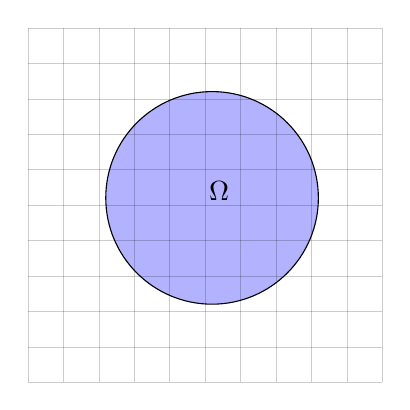
\begin{tikzpicture}[scale=0.9]

            % Domain is blue
            \fill[blue!30] (0.1, 0.1) circle (1.5cm);
            \draw[black] (0.1, 0.1) circle (1.5cm);
            \node at (0.2, 0.2) {$\Omega$};

            % Background mesh
            \foreach \i in {-2.5, -2, ..., 2.5} {
                \draw[line width=0.1pt, shift={(-2.5,\i)}, opacity=0.2] (0,0) -- (5,0);
                \draw[line width=0.1pt, shift={(\i,-2.5)},opacity=0.2] (0,0) -- (0,5);
            }

        \end{tikzpicture}

}\hfill
\subfloat[]{\label{sub:fig:refine_b}
        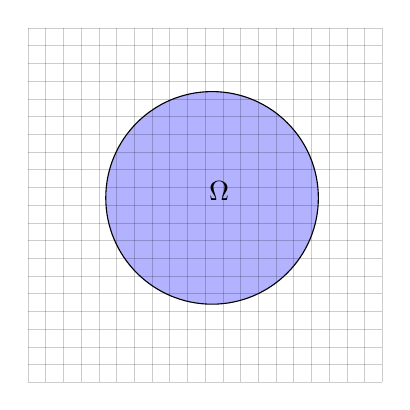
\begin{tikzpicture}[scale=0.9]

            % Domain is blue
            \fill[blue!30] (0.1, 0.1) circle (1.5cm);
            \draw[black] (0.1, 0.1) circle (1.5cm);
            \node at (0.2, 0.2) {$\Omega$};

            % Background mesh
            \foreach \i in {-2.5, -2.25, ..., 2.5} {
                \draw[line width=0.1pt, shift={(-2.5,\i)}, opacity=0.2] (0,0) -- (5,0);
                \draw[line width=0.1pt, shift={(\i,-2.5)},opacity=0.2] (0,0) -- (0,5);
            }

        \end{tikzpicture}


}
\hfill
\subfloat[]{\label{sub:fig:refine_c}
        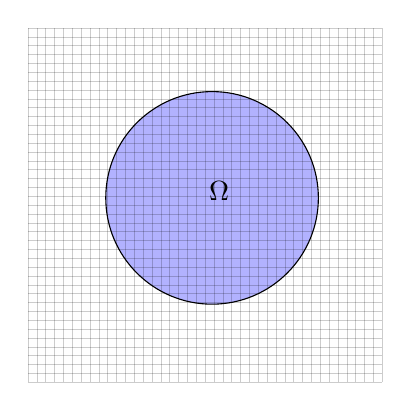
\begin{tikzpicture}[scale=0.9]

            % Domain is blue
            \fill[blue!30] (0.1, 0.1) circle (1.5cm);
            \draw[black] (0.1, 0.1) circle (1.5cm);
            \node at (0.2, 0.2) {$\Omega$};

            % Background mesh
            \foreach \i in {-2.5, -2.375, ..., 2.5} {
                \draw[line width=0.1pt, shift={(-2.5,\i)}, opacity=0.2] (0,0) -- (5,0);
                \draw[line width=0.1pt, shift={(\i,-2.5)},opacity=0.2] (0,0) -- (0,5);
            }

        \end{tikzpicture}
}
    \caption{Illustration of the domain $\Omega $ defined as a circle with radius $R$. The background mesh is a square domain with side lengths $L$ with three refinements of the mesh size $h$.}
\end{figure}


Here we consider the manufactured solution $l,r,m = (2, 1, 1) $ s.t.
\[
u_{\text{ex}}(x,y) = \sin\left(\frac{2\pi m}{l}x_1\right)\cos\left(\frac{2\pi r}{l}y\right)
\]
on the flower domain for the Laplace equation. Here is the flower domain described as
 Recall the polar coordinates $r = \sqrt{x^2 + y^2}$ and $\theta = atan( x,y) $. Then we define the flower level set function $\phi$ to be on the form
 \begin{equation}
 \label{eq:flower}
\phi(x, y) = r_0 + r_1  cos(5 \theta) - r = 0
 \end{equation}
Here we define the parameters $r_0= 0.3L$ and $ r_1=0.1L$.
\begin{figure}
    \centering
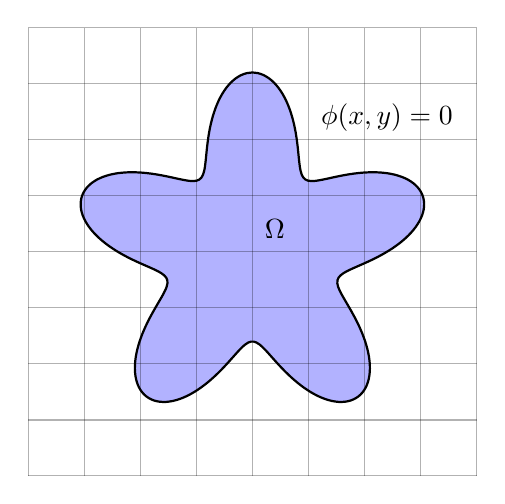
\begin{tikzpicture}
  \def\rZero{0.6} % Define r_0
  \def\rOne{0.2} % Define r_1
  \begin{axis}[
    xmin=-1, xmax=1,
    ymin=-1, ymax=1,
    axis lines=center,
    axis equal,
    hide axis,  % This will hide the axis
    % xlabel={$x$},
    % ylabel={$y$},
    % grid=both,
    % minor tick num=1,
    domain=0:2*pi,
    samples=200
  ]

  \addplot[thick, parametric, smooth, fill=blue!30] ({(\rZero + \rOne*cos(5*deg(x)))*sin(deg(x))} , {(\rZero + \rOne*cos(5*deg(x)))*cos(deg(x))});
  \node at (0.1, 0.1) {$\Omega$};
  \node at (0.6, 0.6) {$\phi( x,y ) = 0 $};

  % Background mesh
  \foreach \i in {-1, -0.75, ..., 1} {
      \addplot[ thin, opacity=0.3, forget plot] coordinates {(\i,-1) (\i,1)};
      \addplot[ thin, opacity=0.3, forget plot] coordinates {(-1,\i) (1,\i)};
  }

  \end{axis}
\end{tikzpicture}
\caption{Illustration of the flower domain associated with the level set function \eqref{eq:flower} s.t. $\phi ( x,y) =0$ for $r_{0} = 0.3L$ and $r_{1} = 0.1L$ }
\end{figure}

\subsubsection{Translation test}%
\label{ssub:translation_test}


Here we have the translation test $\delta $ from $0$ to $2 \sqrt{2}h $.


\begin{figure}
    \centering
    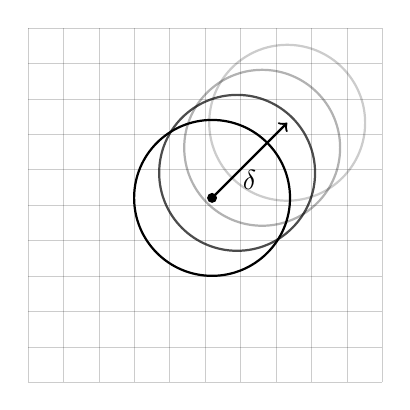
\begin{tikzpicture}[scale=0.9]

        % Domain is blue
        % \fill[blue!30] (0.1, 0.1) circle (1.5cm);

        \coordinate (p0) at (0.1, 0.1);  % the origin of the circle

        \draw[black,line width=0.8pt, opacity=1.0 ] (0.1, 0.1) circle (1.1cm);
        \draw[black,line width=0.8pt, opacity=0.7 ] (0.4535, 0.4535) circle (1.1cm);
        \draw[black,line width=0.8pt, opacity=0.3 ] (0.807, 0.807) circle (1.1cm);
        \draw[black,line width=0.8pt, opacity=0.2 ] (1.16, 1.16) circle (1.1cm);

        % Drawing points
        \fill[black] (p0) circle (2pt);
        \pgfmathsetmacro{\pOneX}{0.1 + 1.5*sqrt(2)*0.5}
        \pgfmathsetmacro{\pOneY}{0.1 + 1.5*sqrt(2)*0.5}
        \coordinate (p1) at (\pOneX, \pOneY);

        \draw[->, thick] (p0) -- (p1) node[midway,below] {$\delta$};
        % Background mesh
        \foreach \i in {-2.5, -2, ..., 2.5} {
            \draw[line width=0.1pt, shift={(-2.5,\i)}, opacity=0.2] (0,0) -- (5,0);
            \draw[line width=0.1pt, shift={(\i,-2.5)},opacity=0.2] (0,0) -- (0,5);
        }

    \end{tikzpicture}
    \caption{Illustration of the translation test with translation $\delta$ from  $(0,2 \sqrt{2}h)  $ }
\end{figure}


\begin{figure}[htp]
\centering

\subfloat[]{%
% Recommended preamble:
% \usetikzlibrary{arrows.meta}
% \usetikzlibrary{backgrounds}
% \usepgfplotslibrary{patchplots}
% \usepgfplotslibrary{fillbetween}
% \pgfplotsset{%
%     layers/standard/.define layer set={%
%         background,axis background,axis grid,axis ticks,axis lines,axis tick labels,pre main,main,axis descriptions,axis foreground%
%     }{
%         grid style={/pgfplots/on layer=axis grid},%
%         tick style={/pgfplots/on layer=axis ticks},%
%         axis line style={/pgfplots/on layer=axis lines},%
%         label style={/pgfplots/on layer=axis descriptions},%
%         legend style={/pgfplots/on layer=axis descriptions},%
%         title style={/pgfplots/on layer=axis descriptions},%
%         colorbar style={/pgfplots/on layer=axis descriptions},%
%         ticklabel style={/pgfplots/on layer=axis tick labels},%
%         axis background@ style={/pgfplots/on layer=axis background},%
%         3d box foreground style={/pgfplots/on layer=axis foreground},%
%     },
% }

\begin{tikzpicture}[/tikz/background rectangle/.style={fill={rgb,1:red,1.0;green,1.0;blue,1.0}, fill opacity={1.0}, draw opacity={1.0}}, show background rectangle]
\begin{axis}[point meta max={nan}, point meta min={nan}, legend cell align={left}, legend columns={1}, title={}, title style={at={{(0.5,1)}}, anchor={south}, font={{\fontsize{14 pt}{18.2 pt}\selectfont}}, color={rgb,1:red,0.0;green,0.0;blue,0.0}, draw opacity={1.0}, rotate={0.0}, align={center}}, legend style={color={rgb,1:red,0.0;green,0.0;blue,0.0}, draw opacity={1.0}, line width={1}, solid, fill={rgb,1:red,1.0;green,1.0;blue,1.0}, fill opacity={1.0}, text opacity={1.0}, font={{\fontsize{12 pt}{15.600000000000001 pt}\selectfont}}, text={rgb,1:red,0.0;green,0.0;blue,0.0}, cells={anchor={center}}, at={(1.02, 1)}, anchor={north west}}, axis background/.style={fill={rgb,1:red,1.0;green,1.0;blue,1.0}, opacity={1.0}}, anchor={north west}, xshift={1.0mm}, yshift={-1.0mm}, width={145.4mm}, height={48.8mm}, scaled x ticks={false}, xlabel={}, x tick style={color={rgb,1:red,0.0;green,0.0;blue,0.0}, opacity={1.0}}, x tick label style={color={rgb,1:red,0.0;green,0.0;blue,0.0}, opacity={1.0}, rotate={0}}, xlabel style={at={(ticklabel cs:0.5)}, anchor=near ticklabel, at={{(ticklabel cs:0.5)}}, anchor={near ticklabel}, font={{\fontsize{11 pt}{14.3 pt}\selectfont}}, color={rgb,1:red,0.0;green,0.0;blue,0.0}, draw opacity={1.0}, rotate={0.0}}, xmajorgrids={true}, xmin={-0.014318912319027599}, xmax={0.49161598961994724}, xticklabels={{$0.0$,$0.1$,$0.2$,$0.3$,$0.4$}}, xtick={{0.0,0.1,0.2,0.30000000000000004,0.4}}, xtick align={inside}, xticklabel style={font={{\fontsize{8 pt}{10.4 pt}\selectfont}}, color={rgb,1:red,0.0;green,0.0;blue,0.0}, draw opacity={1.0}, rotate={0.0}}, x grid style={color={rgb,1:red,0.0;green,0.0;blue,0.0}, draw opacity={0.1}, line width={0.5}, solid}, axis x line*={left}, x axis line style={color={rgb,1:red,0.0;green,0.0;blue,0.0}, draw opacity={1.0}, line width={1}, solid}, scaled y ticks={false}, ylabel={}, y tick style={color={rgb,1:red,0.0;green,0.0;blue,0.0}, opacity={1.0}}, y tick label style={color={rgb,1:red,0.0;green,0.0;blue,0.0}, opacity={1.0}, rotate={0}}, ylabel style={at={(ticklabel cs:0.5)}, anchor=near ticklabel, at={{(ticklabel cs:0.5)}}, anchor={near ticklabel}, font={{\fontsize{11 pt}{14.3 pt}\selectfont}}, color={rgb,1:red,0.0;green,0.0;blue,0.0}, draw opacity={1.0}, rotate={0.0}}, ymode={log}, log basis y={10}, ymajorgrids={true}, ymin={0.20417379446695233}, ymax={4.8977881936844765e23}, yticklabels={{$10^{0}$,$10^{5}$,$10^{10}$,$10^{15}$,$10^{20}$}}, ytick={{1.0,100000.0,1.0e10,1.0e15,1.0e20}}, ytick align={inside}, yticklabel style={font={{\fontsize{8 pt}{10.4 pt}\selectfont}}, color={rgb,1:red,0.0;green,0.0;blue,0.0}, draw opacity={1.0}, rotate={0.0}}, y grid style={color={rgb,1:red,0.0;green,0.0;blue,0.0}, draw opacity={0.1}, line width={0.5}, solid}, axis y line*={left}, y axis line style={color={rgb,1:red,0.0;green,0.0;blue,0.0}, draw opacity={1.0}, line width={1}, solid}, colorbar={false}]
    [\addlegendimage{empty legend}] \addlegendentry[font={{\fontsize{11 pt}{14.3 pt}\selectfont}}, text={rgb,1:red,0.0;green,0.0;blue,0.0}] {\hspace{-.6cm}{\textbf{$(\gamma, \gamma_1, \gamma_2)$}}}
    \addplot[color={rgb,1:red,0.0;green,0.0;blue,1.0}, name path={6b6e567c-0536-4ccb-85ac-ff2f726f8688}, draw opacity={1.0}, line width={1}, solid]
        table[row sep={\\}]
        {
            \\
            0.0  2.4570950441198234e7  \\
            0.0009565071689397187  2.4575177817058776e7  \\
            0.0019130143378794373  2.457939432153537e7  \\
            0.002869521506819156  2.458359993262882e7  \\
            0.0038260286757588746  2.458779465674972e7  \\
            0.004782535844698593  2.4591978499855544e7  \\
            0.005739043013638312  2.459615149276407e7  \\
            0.0066955501825780315  2.4600313711532637e7  \\
            0.007652057351517749  2.4604465240478504e7  \\
            0.008608564520457468  2.4608606200320814e7  \\
            0.009565071689397187  2.461273674546548e7  \\
            0.010521578858336907  2.4616857075354844e7  \\
            0.011478086027276624  2.462096741405805e7  \\
            0.012434593196216343  2.4625068048178114e7  \\
            0.013391100365156063  2.4629159291351434e7  \\
            0.01434760753409578  2.4633241499038637e7  \\
            0.015304114703035498  2.4637315092569552e7  \\
            0.016260621871975217  2.4641380518918514e7  \\
            0.017217129040914936  2.907160783788938e7  \\
            0.018173636209854658  3.01736550733328e7  \\
            0.019130143378794373  3.0161159674663432e7  \\
            0.020086650547734092  3.014553019906001e7  \\
            0.021043157716673814  3.0126793965248656e7  \\
            0.02199966488561353  3.0104971701026954e7  \\
            0.022956172054553248  3.008007733370636e7  \\
            0.02391267922349297  3.0052119811621603e7  \\
            0.024869186392432685  3.0021104900275115e7  \\
            0.025825693561372404  2.9987036114925243e7  \\
            0.026782200730312126  2.9949914985242825e7  \\
            0.027738707899251844  2.9909740491733182e7  \\
            0.02869521506819156  2.9866507994435318e7  \\
            0.02965172223713128  2.9820208143328153e7  \\
            0.030608229406070997  2.9921530302125357e7  \\
            0.031564736575010716  3.004689185085508e7  \\
            0.032521243743950434  3.0102519944424547e7  \\
            0.03347775091289015  3.0075287682572857e7  \\
            0.03443425808182987  3.00129865087198e7  \\
            0.0353907652507696  2.9947594719055988e7  \\
            0.036347272419709316  2.988531269685183e7  \\
            0.03730377958864903  2.999752899209736e7  \\
            0.038260286757588746  3.0099219153132316e7  \\
            0.039216793926528465  3.0190026228974443e7  \\
            0.040173301095468184  3.0269684739036746e7  \\
            0.04112980826440791  3.0338010495639905e7  \\
            0.04208631543334763  3.039489075425501e7  \\
            0.043042822602287346  3.0440274686266273e7  \\
            0.04399932977122706  3.0474454318662822e7  \\
            0.04495583694016678  3.0497795129235696e7  \\
            0.045912344109106495  3.0341716710751604e7  \\
            0.046868851278046214  3.0771626401125457e7  \\
            0.04782535844698594  3.076151458712502e7  \\
            0.04878186561592566  3.0749446394353345e7  \\
            0.04973837278486537  3.073509797094306e7  \\
            0.05069487995380509  3.0718203611125216e7  \\
            0.05165138712274481  3.069876201103822e7  \\
            0.052607894291684526  3.06767678203732e7  \\
            0.05356440146062425  3.0652212190914962e7  \\
            0.05452090862956397  3.0625083300759733e7  \\
            0.05547741579850369  3.0595366822776075e7  \\
            0.0564339229674434  3.056304643253768e7  \\
            0.05739043013638312  3.0528104234280046e7  \\
            0.05834693730532284  3.049052128220792e7  \\
            0.05930344447426256  3.0335482560209706e7  \\
            0.060259951643202275  3.0331179618278597e7  \\
            0.061216458812141994  3.0326477862591956e7  \\
            0.06217296598108171  3.032137135337371e7  \\
            0.06312947315002143  3.0315854469616923e7  \\
            0.06408598031896115  3.0309922067050803e7  \\
            0.06504248748790087  3.0303569589425206e7  \\
            0.06599899465684059  3.0296793219212066e7  \\
            0.0669555018257803  3.0289589822027303e7  \\
            0.06791200899472002  3.0284066007855423e7  \\
            0.06886851616365974  3.0278268767731234e7  \\
            0.06982502333259948  3.027204638185062e7  \\
            0.0707815305015392  3.026539292424087e7  \\
            0.07173803767047891  3.0258609103185315e7  \\
            0.07269454483941863  3.025252874422468e7  \\
            0.07365105200835834  3.026546132730754e7  \\
            0.07460755917729806  3.0282587366997167e7  \\
            0.07556406634623777  3.0290099721479796e7  \\
            0.07652057351517749  3.0707451620736662e7  \\
            0.07747708068411721  3.0714726576558206e7  \\
            0.07843358785305693  3.071931162905674e7  \\
            0.07939009502199665  3.0721196993066136e7  \\
            0.08034660219093637  3.0720367076699384e7  \\
            0.08130310935987609  3.112420066965612e7  \\
            0.08225961652881582  3.1108195263269275e7  \\
            0.08321612369775554  3.1091651801831283e7  \\
            0.08417263086669526  3.1074561353713505e7  \\
            0.08512913803563497  3.1056914988972094e7  \\
            0.08608564520457469  3.103870374273628e7  \\
            0.0870421523735144  3.1019918641520966e7  \\
            0.08799865954245412  3.1000550734756198e7  \\
            0.08895516671139383  3.098059106057635e7  \\
            0.08991167388033355  3.0960030676214512e7  \\
            0.09086818104927327  3.093886065484303e7  \\
            0.09182468821821299  3.091707213473941e7  \\
            0.09278119538715271  3.0894656260436695e7  \\
            0.09373770255609243  3.0871604273380786e7  \\
            0.09469420972503216  3.0847907456246473e7  \\
            0.09565071689397188  3.082355716856913e7  \\
            0.0966072240629116  3.0798544869435646e7  \\
            0.09756373123185132  3.077286208489275e7  \\
            0.09852023840079104  3.0802839391262364e7  \\
            0.09947674556973074  3.0794974625745077e7  \\
            0.10043325273867046  3.0782357008080017e7  \\
            0.10138975990761018  3.076508009316329e7  \\
            0.1023462670765499  3.0743226851306308e7  \\
            0.10330277424548961  3.0716871362234257e7  \\
            0.10425928141442933  3.068608048380502e7  \\
            0.10521578858336905  3.0650915350635044e7  \\
            0.10617229575230877  3.0611432740062624e7  \\
            0.1071288029212485  3.0567686386869814e7  \\
            0.10808531009018822  3.0519728125949744e7  \\
            0.10904181725912794  3.0467608958313305e7  \\
            0.10999832442806766  3.0411380024363186e7  \\
            0.11095483159700738  3.0351093489779077e7  \\
            0.1119113387659471  3.028680333180436e7  \\
            0.1128678459348868  3.021856601931354e7  \\
            0.11382435310382652  3.0146441204509348e7  \\
            0.11478086027276624  3.0070492202054854e7  \\
            0.11573736744170596  2.999078653415546e7  \\
            0.11669387461064568  2.990739633085573e7  \\
            0.1176503817795854  2.9820398654502526e7  \\
            0.11860688894852511  2.9729875815354533e7  \\
            0.11956339611746483  2.9683319727943894e7  \\
            0.12051990328640455  2.9775572556039862e7  \\
            0.12147641045534427  2.986434344364219e7  \\
            0.12243291762428399  2.994954734457105e7  \\
            0.1233894247932237  3.0031104590266336e7  \\
            0.12434593196216343  3.0108940642423145e7  \\
            0.12530243913110314  3.0182985717834253e7  \\
            0.12625894630004286  3.025317446277133e7  \\
            0.12721545346898258  3.0319445441135745e7  \\
            0.1281719606379223  3.0381740672812056e7  \\
            0.12912846780686202  3.044000502522762e7  \\
            0.13008497497580174  3.0494185508416772e7  \\
            0.13104148214474146  3.054423058240205e7  \\
            0.13199798931368117  3.0590089297724113e7  \\
            0.1329544964826209  3.0631710350395396e7  \\
            0.1339110036515606  3.0669041105470937e7  \\
            0.13486751082050033  3.070202644595319e7  \\
            0.13582401798944005  3.073060759898191e7  \\
            0.13678052515837977  3.075472073663347e7  \\
            0.1377370323273195  3.0774295582931016e7  \\
            0.13869353949625923  3.0789253838792805e7  \\
            0.13965004666519895  3.0799507466265783e7  \\
            0.14060655383413867  3.0759766658113934e7  \\
            0.1415630610030784  3.0785787822977725e7  \\
            0.1425195681720181  3.0811134324066084e7  \\
            0.14347607534095783  3.083581455384143e7  \\
            0.14443258250989754  3.085983702791809e7  \\
            0.14538908967883726  3.088321034622242e7  \\
            0.14634559684777695  3.0905943185495753e7  \\
            0.14730210401671667  3.0928044278174613e7  \\
            0.1482586111856564  3.094952244300753e7  \\
            0.1492151183545961  3.0970386527896952e7  \\
            0.15017162552353583  3.099064544400026e7  \\
            0.15112813269247555  3.1010308113748e7  \\
            0.15208463986141527  3.1029383498960465e7  \\
            0.15304114703035498  3.1047880543252785e7  \\
            0.1539976541992947  3.1065808235873237e7  \\
            0.15495416136823442  3.1083175516989663e7  \\
            0.15591066853717414  3.1099991353891876e7  \\
            0.15686717570611386  3.1116264672947556e7  \\
            0.15782368287505358  3.071892721989415e7  \\
            0.1587801900439933  3.072112263113543e7  \\
            0.15973669721293302  3.0720592560371246e7  \\
            0.16069320438187273  3.071735578501008e7  \\
            0.16164971155081245  3.0711424902309578e7  \\
            0.16260621871975217  3.070280701640095e7  \\
            0.16356272588869192  3.028756890506517e7  \\
            0.16451923305763164  3.027520267830903e7  \\
            0.16547574022657136  3.0253408298281793e7  \\
            0.16643224739551107  3.0255624442407522e7  \\
            0.1673887545644508  3.026190263755165e7  \\
            0.1683452617333905  3.026877392038857e7  \\
            0.16930176890233023  3.027521109110161e7  \\
            0.17025827607126995  3.028122016581096e7  \\
            0.17121478324020967  3.0286807018515814e7  \\
            0.17217129040914939  3.0293245076011453e7  \\
            0.17312779757808908  3.0300234606798284e7  \\
            0.1740843047470288  3.0306798598103933e7  \\
            0.1750408119159685  3.0312940514241602e7  \\
            0.17599731908490823  3.0318664549035527e7  \\
            0.17695382625384795  3.0323975562352255e7  \\
            0.17791033342278767  3.0328878969629582e7  \\
            0.1788668405917274  3.0333380566261657e7  \\
            0.1798233477606671  3.047073344989923e7  \\
            0.18077985492960683  3.0509644111982655e7  \\
            0.18173636209854654  3.0545904257205084e7  \\
            0.18269286926748626  3.0579533241080735e7  \\
            0.18364937643642598  3.0610549524144746e7  \\
            0.1846058836053657  3.063897028156015e7  \\
            0.18556239077430542  3.066481089942761e7  \\
            0.18651889794324514  3.068808450350587e7  \\
            0.18747540511218486  3.070880149652774e7  \\
            0.18843191228112458  3.0726969055326845e7  \\
            0.18938841945006432  3.0742590559392318e7  \\
            0.19034492661900404  3.0755665084410887e7  \\
            0.19130143378794376  3.0766890594557967e7  \\
            0.19225794095688348  3.033877680218117e7  \\
            0.1932144481258232  3.0344449802868787e7  \\
            0.19417095529476291  3.0487550792879924e7  \\
            0.19512746246370263  3.0458654324025735e7  \\
            0.19608396963264235  3.0419020755771715e7  \\
            0.19704047680158207  3.0367885808494892e7  \\
            0.1979969839705218  3.0305272795080584e7  \\
            0.19895349113946148  3.02312623205531e7  \\
            0.1999099983084012  3.014600165498742e7  \\
            0.20086650547734092  3.004971437743299e7  \\
            0.20182301264628064  2.9942710415348355e7  \\
            0.20277951981522035  2.9913742699475113e7  \\
            0.20373602698416007  2.998067646755411e7  \\
            0.2046925341530998  3.0044523909437925e7  \\
            0.2056490413220395  3.0105277288137622e7  \\
            0.20660554849097923  3.008417027192958e7  \\
            0.20756205565991895  2.9992178280128945e7  \\
            0.20851856282885867  2.983644933996319e7  \\
            0.20947506999779839  2.984374228712415e7  \\
            0.2104315771667381  2.9888506993970137e7  \\
            0.21138808433567782  2.9930209627512947e7  \\
            0.21234459150461754  2.9968857126821715e7  \\
            0.21330109867355726  3.0004452133418042e7  \\
            0.214257605842497  3.0036994294982463e7  \\
            0.21521411301143673  3.00664810884507e7  \\
            0.21617062018037644  3.0092907918077253e7  \\
            0.21712712734931616  3.0116267612076912e7  \\
            0.21808363451825588  3.0136548989436653e7  \\
            0.2190401416871956  3.015373489637281e7  \\
            0.21999664885613532  3.0167801020986613e7  \\
            0.22095315602507504  2.907045198528429e7  \\
            0.22190966319401476  2.90719838190647e7  \\
            0.22286617036295447  2.4639348789469156e7  \\
            0.2238226775318942  2.4635279345810197e7  \\
            0.2247791847008339  2.4631201497335e7  \\
            0.2257356918697736  2.4627114818020053e7  \\
            0.22669219903871332  2.4623018926657304e7  \\
            0.22764870620765304  2.4618913472579613e7  \\
            0.22860521337659276  2.4614798167866807e7  \\
            0.22956172054553248  2.4610672760244556e7  \\
            0.2305182277144722  2.4606537028148998e7  \\
            0.23147473488341191  2.460239080608322e7  \\
            0.23243124205235163  2.4598233943630286e7  \\
            0.23338774922129135  2.459406634688763e7  \\
            0.23434425639023107  2.4589887935538877e7  \\
            0.2353007635591708  2.4585698650929164e7  \\
            0.2362572707281105  2.4581498485237643e7  \\
            0.23721377789705023  2.457728742830275e7  \\
            0.23817028506598995  2.4573065485630758e7  \\
            0.23912679223492966  2.4573065482373662e7  \\
            0.24008329940386938  2.457728742529129e7  \\
            0.2410398065728091  2.4581498486895002e7  \\
            0.24199631374174882  2.458569865382936e7  \\
            0.24295282091068854  2.4589887935241114e7  \\
            0.24390932807962826  2.459406634834946e7  \\
            0.24486583524856798  2.4598233948105216e7  \\
            0.2458223424175077  2.460239080223208e7  \\
            0.2467788495864474  2.46065370279639e7  \\
            0.24773535675538713  2.4610672756986853e7  \\
            0.24869186392432685  2.461479817131057e7  \\
            0.24964837109326657  2.461891347184445e7  \\
            0.2506048782622063  2.4623018923826165e7  \\
            0.25156138543114603  2.4627114818794254e7  \\
            0.2525178926000857  2.4631201500742715e7  \\
            0.25347439976902547  2.4635279346763823e7  \\
            0.25443090693796516  2.4639348795084365e7  \\
            0.2553874141069049  2.9071983783845942e7  \\
            0.2563439212758446  2.9070451950598136e7  \\
            0.25730042844478435  3.01678009788245e7  \\
            0.25825693561372404  3.0153734865744185e7  \\
            0.2592134427826638  3.0136548951409586e7  \\
            0.2601699499516035  3.0116267571264926e7  \\
            0.2611264571205432  3.0092907877280835e7  \\
            0.2620829642894829  3.0066481046867378e7  \\
            0.26303947145842266  3.003699426113173e7  \\
            0.26399597862736235  3.0004452094181716e7  \\
            0.2649524857963021  2.9968857093126345e7  \\
            0.2659089929652418  2.99302095937406e7  \\
            0.26686550013418153  2.9888506958824255e7  \\
            0.2678220073031212  2.9843742251627482e7  \\
            0.26877851447206097  2.9836449375373743e7  \\
            0.26973502164100066  2.9992178310932744e7  \\
            0.2706915288099404  3.008417030059203e7  \\
            0.2716480359788801  3.010527725209657e7  \\
            0.27260454314781984  3.0044523874954846e7  \\
            0.27356105031675954  2.9980676430762e7  \\
            0.2745175574856993  2.9913742664578613e7  \\
            0.275474064654639  2.9942710449694216e7  \\
            0.2764305718235787  3.0049714409293562e7  \\
            0.27738707899251847  3.0146001691738196e7  \\
            0.27834358616145816  3.0231262356109045e7  \\
            0.2793000933303979  3.030527281502146e7  \\
            0.2802566004993376  3.0367885833233006e7  \\
            0.28121310766827734  3.04190207692425e7  \\
            0.28216961483721703  3.0458654332807556e7  \\
            0.2831261220061568  3.0487550802924424e7  \\
            0.28408262917509647  3.0344449771424025e7  \\
            0.2850391363440362  3.033877680241027e7  \\
            0.2859956435129759  3.0766890560436744e7  \\
            0.28695215068191565  3.0755665040552486e7  \\
            0.28790865785085534  3.0742590515173417e7  \\
            0.2888651650197951  3.072696901698025e7  \\
            0.2898216721887348  3.0708801464417815e7  \\
            0.2907781793576745  3.068808445893715e7  \\
            0.29173468652661416  3.0664810856705133e7  \\
            0.2926911936955539  3.063897024290705e7  \\
            0.2936477008644936  3.061054949263729e7  \\
            0.29460420803343335  3.057953319898957e7  \\
            0.29556071520237304  3.0545904219456498e7  \\
            0.2965172223713128  3.050964406797651e7  \\
            0.2974737295402525  3.0470733406598862e7  \\
            0.2984302367091922  3.033338056168998e7  \\
            0.2993867438781319  3.0328878968684807e7  \\
            0.30034325104707166  3.0323975567967772e7  \\
            0.3012997582160114  3.031866454672022e7  \\
            0.3022562653849511  3.03129405027257e7  \\
            0.30321277255389084  3.0306798595403954e7  \\
            0.30416927972283053  3.030023460266286e7  \\
            0.3051257868917703  3.0293245066209886e7  \\
            0.30608229406070997  3.0286807013139594e7  \\
            0.3070388012296497  3.0281220161414873e7  \\
            0.3079953083985894  3.02752110857404e7  \\
            0.30895181556752915  3.026877391659413e7  \\
            0.30990832273646884  3.0261902631018434e7  \\
            0.3108648299054086  3.0255624439983536e7  \\
            0.3118213370743483  3.025340833444095e7  \\
            0.31277784424328803  3.027520270679611e7  \\
            0.3137343514122277  3.0287568941408742e7  \\
            0.31469085858116747  3.0702807055033367e7  \\
            0.31564736575010716  3.0711424937590323e7  \\
            0.3166038729190469  3.071735582099643e7  \\
            0.3175603800879866  3.072059259378963e7  \\
            0.31851688725692634  3.0721122668494757e7  \\
            0.31947339442586603  3.071892725537317e7  \\
            0.3204299015948058  3.111626466844076e7  \\
            0.32138640876374547  3.1099991340138778e7  \\
            0.3223429159326852  3.108317550425999e7  \\
            0.3232994231016249  3.1065808216852106e7  \\
            0.32425593027056465  3.104788053543975e7  \\
            0.32521243743950434  3.1029383479557272e7  \\
            0.3261689446084441  3.1010308099328134e7  \\
            0.32712545177738384  3.0990645428899355e7  \\
            0.3280819589463235  3.097038651052753e7  \\
            0.3290384661152633  3.0949522421516128e7  \\
            0.32999497328420296  3.0928044264919538e7  \\
            0.3309514804531427  3.090594316230229e7  \\
            0.3319079876220824  3.0883210333416384e7  \\
            0.33286449479102215  3.0859837008729413e7  \\
            0.33382100195996184  3.083581453549271e7  \\
            0.3347775091289016  3.08111342973057e7  \\
            0.3357340162978413  3.078578780087762e7  \\
            0.336690523466781  3.0759766639093738e7  \\
            0.3376470306357207  3.0799507427978713e7  \\
            0.33860353780466046  3.0789253806501605e7  \\
            0.33956004497360015  3.0774295549455315e7  \\
            0.3405165521425399  3.0754720695578974e7  \\
            0.3414730593114796  3.0730607564238086e7  \\
            0.34242956648041933  3.0702026408382367e7  \\
            0.343386073649359  3.0669041059616394e7  \\
            0.34434258081829877  3.063171031172745e7  \\
            0.3452990879872384  3.059008925423312e7  \\
            0.34625559515617815  3.054423055075131e7  \\
            0.34721210232511784  3.0494185467334226e7  \\
            0.3481686094940576  3.0440004982362393e7  \\
            0.3491251166629973  3.038174063866572e7  \\
            0.350081623831937  3.0319445397941872e7  \\
            0.3510381310008768  3.0253174418414272e7  \\
            0.35199463816981647  3.018298568030272e7  \\
            0.3529511453387562  3.010894060455665e7  \\
            0.3539076525076959  3.0031104558951944e7  \\
            0.35486415967663565  2.9949547302579995e7  \\
            0.35582066684557534  2.9864343409090124e7  \\
            0.3567771740145151  2.9775572524318885e7  \\
            0.3577336811834548  2.9683319683590423e7  \\
            0.3586901883523945  2.9729875851715174e7  \\
            0.3596466955213342  2.9820398684070054e7  \\
            0.36060320269027396  2.9907396364054307e7  \\
            0.36155970985921365  2.999078657556043e7  \\
            0.3625162170281534  3.007049223366633e7  \\
            0.3634727241970931  3.014644123456949e7  \\
            0.36442923136603284  3.021856606096142e7  \\
            0.3653857385349725  3.0286803367960364e7  \\
            0.3663422457039123  3.0351093533642422e7  \\
            0.36729875287285196  3.0411380058893193e7  \\
            0.3682552600417917  3.0467608989377838e7  \\
            0.3692117672107314  3.051972815728923e7  \\
            0.37016827437967115  3.0567686423309222e7  \\
            0.37112478154861084  3.0611432771321993e7  \\
            0.3720812887175506  3.0650915386305217e7  \\
            0.3730377958864903  3.0686080518180557e7  \\
            0.37399430305543  3.0716871399124347e7  \\
            0.3749508102243697  3.0743226886467367e7  \\
            0.37590731739330946  3.076508012939139e7  \\
            0.37686382456224915  3.0782357036973022e7  \\
            0.3778203317311889  3.079497466202439e7  \\
            0.37877683890012864  3.0802839425481606e7  \\
            0.37973334606906833  3.0772862095347285e7  \\
            0.3806898532380081  3.079854488607746e7  \\
            0.38164636040694777  3.082355719096101e7  \\
            0.3826028675758875  3.0847907471594803e7  \\
            0.3835593747448272  3.0871604297254715e7  \\
            0.38451588191376695  3.0894656282668184e7  \\
            0.38547238908270665  3.0917072144794162e7  \\
            0.3864288962516464  3.0938860675577164e7  \\
            0.3873854034205861  3.0960030692258693e7  \\
            0.38834191058952583  3.09805910728807e7  \\
            0.3892984177584655  3.1000550753608078e7  \\
            0.39025492492740527  3.1019918659720954e7  \\
            0.39121143209634496  3.1038703754629113e7  \\
            0.3921679392652847  3.1056914996125918e7  \\
            0.3931244464342244  3.1074561370037157e7  \\
            0.39408095360316414  3.1091651805671602e7  \\
            0.39503746077210383  3.1108195271524064e7  \\
            0.3959939679410436  3.1124200679101568e7  \\
            0.39695047510998327  3.0720367044622265e7  \\
            0.39790698227892296  3.07211969570261e7  \\
            0.39886348944786265  3.0719311586340696e7  \\
            0.3998199966168024  3.0714726537941653e7  \\
            0.4007765037857421  3.070745157826378e7  \\
            0.40173301095468184  3.0290099680435043e7  \\
            0.4026895181236216  3.0282587324158646e7  \\
            0.4036460252925613  3.026546128350644e7  \\
            0.404602532461501  3.025252874853202e7  \\
            0.4055590396304407  3.0258609105273053e7  \\
            0.40651554679938046  3.0265392930485714e7  \\
            0.40747205396832015  3.0272046386204123e7  \\
            0.4084285611372599  3.0278268772783525e7  \\
            0.4093850683061996  3.028406601181682e7  \\
            0.41034157547513933  3.028958982317097e7  \\
            0.411298082644079  3.029679322055194e7  \\
            0.41225458981301877  3.0303569598112736e7  \\
            0.41321109698195846  3.0309922068390656e7  \\
            0.4141676041508982  3.031585447098303e7  \\
            0.4151241113198379  3.0321371358573902e7  \\
            0.41608061848877764  3.0326477868632194e7  \\
            0.41703712565771733  3.0331179618346915e7  \\
            0.4179936328266571  3.0335482557138223e7  \\
            0.41895013999559677  3.0490521318382397e7  \\
            0.4199066471645365  3.0528104272652082e7  \\
            0.4208631543334762  3.0563046463415507e7  \\
            0.42181966150241595  3.0595366856836822e7  \\
            0.42277616867135565  3.062508333946821e7  \\
            0.4237326758402954  3.065221222926261e7  \\
            0.4246891830092351  3.0676767850883096e7  \\
            0.42564569017817483  3.0698762046829924e7  \\
            0.4266021973471145  3.071820364809627e7  \\
            0.42755870451605427  3.073509800733173e7  \\
            0.428515211684994  3.0749446428056683e7  \\
            0.4294717188539337  3.0761514622226343e7  \\
            0.43042822602287345  3.0771626430848684e7  \\
            0.43138473319181314  3.0341716742912374e7  \\
            0.4323412403607529  3.0497795118115388e7  \\
            0.4332977475296926  3.04744543101396e7  \\
            0.4342542546986323  3.0440274669962056e7  \\
            0.435210761867572  3.039489073781782e7  \\
            0.43616726903651176  3.033801047451784e7  \\
            0.43712377620545145  3.026968470659531e7  \\
            0.4380802833743912  3.0190026198443636e7  \\
            0.4390367905433309  3.0099219119303986e7  \\
            0.43999329771227064  2.999752896140491e7  \\
            0.4409498048812103  2.9885312654516544e7  \\
            0.4419063120501501  2.9947594754010115e7  \\
            0.44286281921908976  3.001298654301016e7  \\
            0.4438193263880295  3.0075287713397577e7  \\
            0.4447758335569692  3.010251990591001e7  \\
            0.44573234072590895  3.004689181892752e7  \\
            0.44668884789484864  2.9921530265269466e7  \\
            0.4476453550637884  2.982020817819402e7  \\
            0.4486018622327281  2.9866508027666938e7  \\
            0.4495583694016678  2.9909740526872296e7  \\
            0.4505148765706075  2.9949915016551923e7  \\
            0.4514713837395472  2.9987036150972072e7  \\
            0.45242789090848695  3.0021104930279184e7  \\
            0.45338439807742664  3.0052119847611327e7  \\
            0.4543409052463664  3.0080077370535545e7  \\
            0.4552974124153061  3.0104971734610923e7  \\
            0.4562539195842458  3.0126793994229548e7  \\
            0.4572104267531855  3.014553022954214e7  \\
            0.45816693392212526  3.0161159707895633e7  \\
            0.45912344109106495  3.0173655108579237e7  \\
            0.4600799482600047  2.907160786676577e7  \\
            0.4610364554289444  2.4641380512272116e7  \\
            0.46199296259788414  2.463731508761835e7  \\
            0.46294946976682383  2.463324150187979e7  \\
            0.4639059769357636  2.462915928578683e7  \\
            0.46486248410470327  2.4625068044178445e7  \\
            0.465818991273643  2.4620967416665543e7  \\
            0.4667754984425827  2.4616857067734804e7  \\
            0.46773200561152245  2.461273673887529e7  \\
            0.46868851278046214  2.4608606194144487e7  \\
            0.4696450199494019  2.4604465234844e7  \\
            0.4706015271183416  2.4600313714814134e7  \\
            0.4715580342872813  2.459615149524198e7  \\
            0.472514541456221  2.4591978496477418e7  \\
            0.47347104862516076  2.4587794650482167e7  \\
            0.47442755579410045  2.45835999353068e7  \\
            0.4753840629630402  2.4579394320014752e7  \\
            0.4763405701319799  2.4575177812048133e7  \\
            0.47729707730091964  2.4570950435266025e7  \\
        }
        ;
    \addlegendentry {$(20.0, 10.0, 0.5) $}
    \addplot[color={rgb,1:red,1.0;green,0.0;blue,0.0}, name path={c8b1aeb1-58b2-4cb9-ab42-5a47cc9639fc}, draw opacity={1.0}, line width={1}, solid]
        table[row sep={\\}]
        {
            \\
            0.0  8.939008519076015e9  \\
            0.0009565071689397187  1.3826755787084549e10  \\
            0.0019130143378794373  2.1845573828891613e10  \\
            0.002869521506819156  3.538174415400113e10  \\
            0.0038260286757588746  5.8993659861484276e10  \\
            0.004782535844698593  1.0177583977302077e11  \\
            0.005739043013638312  1.8282061669420212e11  \\
            0.0066955501825780315  3.446639302476399e11  \\
            0.007652057351517749  6.89042815846331e11  \\
            0.008608564520457468  1.4804593582444592e12  \\
            0.009565071689397187  3.4851347619935e12  \\
            0.010521578858336907  9.236258543164941e12  \\
            0.011478086027276624  2.8720547666490316e13  \\
            0.012434593196216343  1.1210196377109917e14  \\
            0.013391100365156063  6.203310260652621e14  \\
            0.01434760753409578  6.291201174936238e15  \\
            0.015304114703035498  2.4025306959790736e17  \\
            0.016260621871975217  3.55470011833026e21  \\
            0.017217129040914936  7.785483774539897e10  \\
            0.018173636209854658  2.996175105921447e16  \\
            0.019130143378794373  3.588855389296854e13  \\
            0.020086650547734092  2.035004609196768e12  \\
            0.021043157716673814  3.1169748548576184e11  \\
            0.02199966488561353  1.6805173352975668e11  \\
            0.022956172054553248  1.9834396781299347e11  \\
            0.02391267922349297  2.3514235775175546e11  \\
            0.024869186392432685  2.8008142360864594e11  \\
            0.025825693561372404  3.352710693984947e11  \\
            0.026782200730312126  4.034519664406695e11  \\
            0.027738707899251844  4.8821275052523566e11  \\
            0.02869521506819156  5.942896068316727e11  \\
            0.02965172223713128  7.279864851202438e11  \\
            0.030608229406070997  8.97770034122171e11  \\
            0.031564736575010716  1.1151215289547913e12  \\
            0.032521243743950434  1.3957706584429585e12  \\
            0.03347775091289015  7.331095137519722e16  \\
            0.03443425808182987  5.726433923219986e14  \\
            0.0353907652507696  4.413350665252235e13  \\
            0.036347272419709316  7.709867950139438e12  \\
            0.03730377958864903  4.918922352527987e12  \\
            0.038260286757588746  6.540412630540542e12  \\
            0.039216793926528465  8.81332243490471e12  \\
            0.040173301095468184  2.2038707928091516e13  \\
            0.04112980826440791  7.905020691219112e13  \\
            0.04208631543334763  3.863276708726628e14  \\
            0.043042822602287346  3.181028598630001e15  \\
            0.04399932977122706  7.67895260921663e16  \\
            0.04495583694016678  7.702821455234086e19  \\
            0.045912344109106495  1.1898364914478716e14  \\
            0.046868851278046214  1.0e23  \\
            0.04782535844698594  3.591128470196195e17  \\
            0.04878186561592566  8.347170780733437e15  \\
            0.04973837278486537  1.0332318833868214e15  \\
            0.05069487995380509  2.0324596669290772e15  \\
            0.05165138712274481  4.3286654245749505e15  \\
            0.052607894291684526  1.0193937556510028e16  \\
            0.05356440146062425  2.7375431702328508e16  \\
            0.05452090862956397  8.792407143649294e16  \\
            0.05547741579850369  3.657711037139831e17  \\
            0.0564339229674434  2.2886999040912635e18  \\
            0.05739043013638312  3.0174786798037524e19  \\
            0.05834693730532284  2.507079648437468e21  \\
            0.05930344447426256  6.413319971353387e11  \\
            0.060259951643202275  5.197635062694138e11  \\
            0.061216458812141994  4.635708839360576e11  \\
            0.06217296598108171  4.873515048735434e11  \\
            0.06312947315002143  9.58510870658198e11  \\
            0.06408598031896115  2.0669078828236188e11  \\
            0.06504248748790087  1.1024039376921675e12  \\
            0.06599899465684059  1.7832277070095862e11  \\
            0.0669555018257803  7.784904239791014e10  \\
            0.06791200899472002  4.190993459346536e10  \\
            0.06886851616365974  2.492979658960681e10  \\
            0.06982502333259948  1.5762747525208256e10  \\
            0.0707815305015392  1.039805904742587e10  \\
            0.07173803767047891  7.080448979150426e9  \\
            0.07269454483941863  4.94349255549799e9  \\
            0.07365105200835834  3.5225793623125157e9  \\
            0.07460755917729806  2.553252163515623e9  \\
            0.07556406634623777  1.8778012403913858e9  \\
            0.07652057351517749  1.8863112925164388e18  \\
            0.07747708068411721  1.1428839127126374e16  \\
            0.07843358785305693  8.93436533829132e14  \\
            0.07939009502199665  1.7319663757546144e14  \\
            0.08034660219093637  5.551828405550436e13  \\
            0.08130310935987609  3.5890161193655007e21  \\
            0.08225961652881582  2.1331931286717658e17  \\
            0.08321612369775554  5.77684600578272e15  \\
            0.08417263086669526  5.880881801127709e14  \\
            0.08512913803563497  1.0910073074500139e14  \\
            0.08608564520457469  2.8560561546684836e13  \\
            0.0870421523735144  9.351881753552654e12  \\
            0.08799865954245412  3.583466857048173e12  \\
            0.08895516671139383  1.5428090897684578e12  \\
            0.08991167388033355  8.870065362011023e11  \\
            0.09086818104927327  2.0438540622339612e12  \\
            0.09182468821821299  5.247966193918293e12  \\
            0.09278119538715271  1.55537970655395e13  \\
            0.09373770255609243  5.62349960543442e13  \\
            0.09469420972503216  2.7260416596308953e14  \\
            0.09565071689397188  2.1264888078442828e15  \\
            0.0966072240629116  4.113125927164131e16  \\
            0.09756373123185132  9.970487192059294e18  \\
            0.09852023840079104  6.685260179500391e9  \\
            0.09947674556973074  4.498524920148409e9  \\
            0.10043325273867046  3.0650881697404766e9  \\
            0.10138975990761018  2.1092175131508179e9  \\
            0.1023462670765499  1.461990625991943e9  \\
            0.10330277424548961  1.0177047419567645e9  \\
            0.10425928141442933  7.08929626481291e8  \\
            0.10521578858336905  4.9188722030327296e8  \\
            0.10617229575230877  3.376907549250713e8  \\
            0.1071288029212485  2.8472631735809135e8  \\
            0.10808531009018822  3.102367849793143e8  \\
            0.10904181725912794  3.416813476194751e8  \\
            0.10999832442806766  3.887957551412766e9  \\
            0.11095483159700738  4.253124966885904e8  \\
            0.1119113387659471  4.833222352996191e8  \\
            0.1128678459348868  5.61743138602973e8  \\
            0.11382435310382652  6.716009031609267e8  \\
            0.11478086027276624  8.357410948807799e8  \\
            0.11573736744170596  1.1066240806914692e9  \\
            0.11669387461064568  1.6363778983017652e9  \\
            0.1176503817795854  3.107029699920634e9  \\
            0.11860688894852511  2.1239921095444874e10  \\
            0.11956339611746483  1.3898858081225788e10  \\
            0.12051990328640455  5.51606715014098e9  \\
            0.12147641045534427  2.147630844542372e9  \\
            0.12243291762428399  1.3204618669572704e9  \\
            0.1233894247932237  9.522842008965001e8  \\
            0.12434593196216343  7.446768016756355e8  \\
            0.12530243913110314  6.117009804762638e8  \\
            0.12625894630004286  5.1947969307288504e8  \\
            0.12721545346898258  4.521549684671089e8  \\
            0.1281719606379223  4.03236432859101e8  \\
            0.12912846780686202  5.354016427797664e8  \\
            0.13008497497580174  3.2499944299956614e8  \\
            0.13104148214474146  2.968927300190607e8  \\
            0.13199798931368117  2.77840565367776e8  \\
            0.1329544964826209  4.0831967059139436e8  \\
            0.1339110036515606  5.910210648783476e8  \\
            0.13486751082050033  8.495450316450083e8  \\
            0.13582401798944005  1.2193834558686647e9  \\
            0.13678052515837977  1.7547541135499775e9  \\
            0.1377370323273195  2.539888402776487e9  \\
            0.13869353949625923  3.7080728491060514e9  \\
            0.13965004666519895  5.474530377005848e9  \\
            0.14060655383413867  3.970279216084333e21  \\
            0.1415630610030784  3.649957542077611e17  \\
            0.1425195681720181  7.957706539463643e15  \\
            0.14347607534095783  7.048960821224888e14  \\
            0.14443258250989754  1.1836062515927497e14  \\
            0.14538908967883726  2.8715387773999113e13  \\
            0.14634559684777695  8.84899105208793e12  \\
            0.14730210401671667  3.2250422047459424e12  \\
            0.1482586111856564  1.330591672755854e12  \\
            0.1492151183545961  1.048350831400494e12  \\
            0.15017162552353583  2.3216969669685884e12  \\
            0.15112813269247555  5.693203341189602e12  \\
            0.15208463986141527  1.5971483457117389e13  \\
            0.15304114703035498  5.3970220555716445e13  \\
            0.1539976541992947  2.399406089147199e14  \\
            0.15495416136823442  1.665670452068793e15  \\
            0.15591066853717414  2.7177448594204284e16  \\
            0.15686717570611386  4.767118441470547e18  \\
            0.15782368287505358  3.6270098287766336e13  \\
            0.1587801900439933  9.318011192054942e13  \\
            0.15973669721293302  3.637650052230261e14  \\
            0.16069320438187273  2.7206020476165125e15  \\
            0.16164971155081245  8.278898632109947e16  \\
            0.16260621871975217  3.170982008768662e21  \\
            0.16356272588869192  2.185937743566649e9  \\
            0.16451923305763164  2.9931319063012733e9  \\
            0.16547574022657136  4.1633357442313323e9  \\
            0.16643224739551107  5.899719870860133e9  \\
            0.1673887545644508  8.550554334646245e9  \\
            0.1683452617333905  1.2744783633035063e10  \\
            0.16930176890233023  1.970078845536606e10  \\
            0.17025827607126995  3.2023277640785427e10  \\
            0.17121478324020967  5.618840146125923e10  \\
            0.17217129040914939  1.1320020820254913e11  \\
            0.17312779757808908  3.311439058297294e11  \\
            0.1740843047470288  9.960007082675403e11  \\
            0.1750408119159685  8.205002480235715e11  \\
            0.17599731908490823  5.747792900343732e11  \\
            0.17695382625384795  4.616065782864312e11  \\
            0.17791033342278767  4.838357632433135e11  \\
            0.1788668405917274  5.715665854299962e11  \\
            0.1798233477606671  1.0e23  \\
            0.18077985492960683  1.880915504455856e20  \\
            0.18173636209854654  7.302170090143355e18  \\
            0.18269286926748626  8.572243612569379e17  \\
            0.18364937643642598  1.724174173049993e17  \\
            0.1846058836053657  4.778576757819e16  \\
            0.18556239077430542  1.6392789204592964e16  \\
            0.18651889794324514  6.549086844182744e15  \\
            0.18747540511218486  2.933447300140283e15  \\
            0.18843191228112458  1.4363250356468668e15  \\
            0.18938841945006432  2.469165093236452e15  \\
            0.19034492661900404  3.934251636460751e16  \\
            0.19130143378794376  1.3107063314234294e19  \\
            0.19225794095688348  1.502950578877144e14  \\
            0.1932144481258232  9.497218714118734e13  \\
            0.19417095529476291  9.636223092038993e17  \\
            0.19512746246370263  1.2797030897787598e16  \\
            0.19608396963264235  1.0167616433720786e15  \\
            0.19704047680158207  1.6654178649726662e14  \\
            0.1979969839705218  4.047887401291157e13  \\
            0.19895349113946148  1.2621765474385648e13  \\
            0.1999099983084012  7.579033497360532e12  \\
            0.20086650547734092  5.662963778379549e12  \\
            0.20182301264628064  4.2857075732441987e12  \\
            0.20277951981522035  1.7217932112436363e13  \\
            0.20373602698416007  1.3732230847964486e14  \\
            0.2046925341530998  3.9114237831312885e15  \\
            0.2056490413220395  3.877325320447809e19  \\
            0.20660554849097923  1.2463404195795527e12  \\
            0.20756205565991895  9.996340515554292e11  \\
            0.20851856282885867  8.07732717236578e11  \\
            0.20947506999779839  6.572155446506666e11  \\
            0.2104315771667381  5.382353744394856e11  \\
            0.21138808433567782  4.434949815971707e11  \\
            0.21234459150461754  3.6753622210994934e11  \\
            0.21330109867355726  3.062406434332074e11  \\
            0.214257605842497  2.5647503694394843e11  \\
            0.21521411301143673  2.158422266682666e11  \\
            0.21617062018037644  1.824714791376804e11  \\
            0.21712712734931616  1.549356813520545e11  \\
            0.21808363451825588  7.360678436284402e11  \\
            0.2190401416871956  7.0902734951026e12  \\
            0.21999664885613532  3.693506569177321e14  \\
            0.22095315602507504  8.374085347065341e10  \\
            0.22190966319401476  7.244225590590582e10  \\
            0.22286617036295447  5.382080475934783e18  \\
            0.2238226775318942  3.012250128709419e16  \\
            0.2247791847008339  1.7838811261471512e15  \\
            0.2257356918697736  2.4962965496134753e14  \\
            0.22669219903871332  5.483273524643095e13  \\
            0.22764870620765304  1.5910806985432812e13  \\
            0.22860521337659276  5.578137813179613e12  \\
            0.22956172054553248  2.242445083580996e12  \\
            0.2305182277144722  9.998296929809229e11  \\
            0.23147473488341191  4.8340932694167505e11  \\
            0.23243124205235163  2.4936483909064435e11  \\
            0.23338774922129135  1.3565838803183849e11  \\
            0.23434425639023107  7.712888740616837e10  \\
            0.2353007635591708  4.550811971692307e10  \\
            0.2362572707281105  2.7708736620728508e10  \\
            0.23721377789705023  1.7329988042644665e10  \\
            0.23817028506598995  1.1090283414452368e10  \\
            0.23912679223492966  1.1090283414139172e10  \\
            0.24008329940386938  1.7329988043978703e10  \\
            0.2410398065728091  2.7708736620775986e10  \\
            0.24199631374174882  4.5508119714886406e10  \\
            0.24295282091068854  7.71288873981817e10  \\
            0.24390932807962826  1.3565838803464e11  \\
            0.24486583524856798  2.4936483914891165e11  \\
            0.2458223424175077  4.8340932651965204e11  \\
            0.2467788495864474  9.998296922018705e11  \\
            0.24773535675538713  2.242445084487568e12  \\
            0.24869186392432685  5.578137795680781e12  \\
            0.24964837109326657  1.5910806973751203e13  \\
            0.2506048782622063  5.483273572025131e13  \\
            0.25156138543114603  2.4962966509762903e14  \\
            0.2525178926000857  1.7838811608314235e15  \\
            0.25347439976902547  3.012250690553355e16  \\
            0.25443090693796516  5.382103226247797e18  \\
            0.2553874141069049  7.244225588394377e10  \\
            0.2563439212758446  8.37408534530838e10  \\
            0.25730042844478435  3.693506341769237e14  \\
            0.25825693561372404  7.090273500198148e12  \\
            0.2592134427826638  7.360678442293765e11  \\
            0.2601699499516035  1.549356813179392e11  \\
            0.2611264571205432  1.824714791204574e11  \\
            0.2620829642894829  2.1584222671034622e11  \\
            0.26303947145842266  2.5647503681358554e11  \\
            0.26399597862736235  3.0624064364909045e11  \\
            0.2649524857963021  3.675362217833041e11  \\
            0.2659089929652418  4.434949810588284e11  \\
            0.26686550013418153  5.3823537376505853e11  \\
            0.2678220073031212  6.572155445410918e11  \\
            0.26877851447206097  8.077327154815587e11  \\
            0.26973502164100066  9.996340504743337e11  \\
            0.2706915288099404  1.2463404167783813e12  \\
            0.2716480359788801  3.8773349413164474e19  \\
            0.27260454314781984  3.911423705650689e15  \\
            0.27356105031675954  1.3732230841341134e14  \\
            0.2745175574856993  1.7217932201631633e13  \\
            0.275474064654639  4.2857075890063604e12  \\
            0.2764305718235787  5.662963799629337e12  \\
            0.27738707899251847  7.579033508704118e12  \\
            0.27834358616145816  1.2621765486422367e13  \\
            0.2793000933303979  4.047887447052634e13  \\
            0.2802566004993376  1.6654178963773938e14  \\
            0.28121310766827734  1.0167616394084674e15  \\
            0.28216961483721703  1.2797029614236274e16  \\
            0.2831261220061568  9.63620661912073e17  \\
            0.28408262917509647  9.497218900385217e13  \\
            0.2850391363440362  1.502950593301985e14  \\
            0.2859956435129759  1.3107142470685385e19  \\
            0.28695215068191565  3.934247711412966e16  \\
            0.28790865785085534  2.46916462134663e15  \\
            0.2888651650197951  1.4363251751567542e15  \\
            0.2898216721887348  2.9334474137693165e15  \\
            0.2907781793576745  6.549086097695477e15  \\
            0.29173468652661416  1.6392788635041996e16  \\
            0.2926911936955539  4.778580170326555e16  \\
            0.2936477008644936  1.724173093563409e17  \\
            0.29460420803343335  8.572224728146414e17  \\
            0.29556071520237304  7.302184110153609e18  \\
            0.2965172223713128  1.8809632043395973e20  \\
            0.2974737295402525  1.0e23  \\
            0.2984302367091922  5.715665868782766e11  \\
            0.2993867438781319  4.838357631939054e11  \\
            0.30034325104707166  4.6160657645445184e11  \\
            0.3012997582160114  5.747792891894912e11  \\
            0.3022562653849511  8.205002500504387e11  \\
            0.30321277255389084  9.960006894733274e11  \\
            0.30416927972283053  3.3114390668372754e11  \\
            0.3051257868917703  1.1320020836855856e11  \\
            0.30608229406070997  5.618840146481923e10  \\
            0.3070388012296497  3.202327764537808e10  \\
            0.3079953083985894  1.9700788460485195e10  \\
            0.30895181556752915  1.2744783631959135e10  \\
            0.30990832273646884  8.550554335050983e9  \\
            0.3108648299054086  5.899719870844479e9  \\
            0.3118213370743483  4.1633357443354e9  \\
            0.31277784424328803  2.9931319063571534e9  \\
            0.3137343514122277  2.185937743780786e9  \\
            0.31469085858116747  3.171199303433156e21  \\
            0.31564736575010716  8.278916507534013e16  \\
            0.3166038729190469  2.7206017795135745e15  \\
            0.3175603800879866  3.637650134421436e14  \\
            0.31851688725692634  9.318011292889261e13  \\
            0.31947339442586603  3.627009841759382e13  \\
            0.3204299015948058  4.767123935370036e18  \\
            0.32138640876374547  2.7177460178967964e16  \\
            0.3223429159326852  1.665670658654935e15  \\
            0.3232994231016249  2.399405991552644e14  \\
            0.32425593027056465  5.3970220281856445e13  \\
            0.32521243743950434  1.597148351345897e13  \\
            0.3261689446084441  5.693203333795265e12  \\
            0.32712545177738384  2.321696959633732e12  \\
            0.3280819589463235  1.0483508325636621e12  \\
            0.3290384661152633  1.3305916731647246e12  \\
            0.32999497328420296  3.225042200001061e12  \\
            0.3309514804531427  8.848991054252979e12  \\
            0.3319079876220824  2.8715387859630863e13  \\
            0.33286449479102215  1.1836062973569095e14  \\
            0.33382100195996184  7.048961892758899e14  \\
            0.3347775091289016  7.957705711363891e15  \\
            0.3357340162978413  3.6499492015346675e17  \\
            0.336690523466781  3.9641470631418837e21  \\
            0.3376470306357207  5.47453037693907e9  \\
            0.33860353780466046  3.708072848927601e9  \\
            0.33956004497360015  2.5398884023105364e9  \\
            0.3405165521425399  1.7547541132923229e9  \\
            0.3414730593114796  1.219383455641906e9  \\
            0.34242956648041933  8.4954503142732e8  \\
            0.343386073649359  5.910210646634351e8  \\
            0.34434258081829877  4.083196704064087e8  \\
            0.3452990879872384  2.778405651850825e8  \\
            0.34625559515617815  2.968927299442431e8  \\
            0.34721210232511784  3.2499944291563976e8  \\
            0.3481686094940576  5.354018906750611e8  \\
            0.3491251166629973  4.032364327089749e8  \\
            0.350081623831937  4.521549682928944e8  \\
            0.3510381310008768  5.194796928264311e8  \\
            0.35199463816981647  6.117009801018426e8  \\
            0.3529511453387562  7.446768011191039e8  \\
            0.3539076525076959  9.522841998868822e8  \\
            0.35486415967663565  1.320461865104572e9  \\
            0.35582066684557534  2.1476308391377506e9  \\
            0.3567771740145151  5.5160671130117035e9  \\
            0.3577336811834548  1.3898858246210106e10  \\
            0.3586901883523945  2.123992157921117e10  \\
            0.3596466955213342  3.10702971164347e9  \\
            0.36060320269027396  1.6363779013641076e9  \\
            0.36155970985921365  1.1066240819771802e9  \\
            0.3625162170281534  8.357410955841044e8  \\
            0.3634727241970931  6.716009036298727e8  \\
            0.36442923136603284  5.617431389073638e8  \\
            0.3653857385349725  4.8332223551624143e8  \\
            0.3663422457039123  4.25312496854842e8  \\
            0.36729875287285196  3.887958542583211e9  \\
            0.3682552600417917  3.4168134770167744e8  \\
            0.3692117672107314  3.102367850581196e8  \\
            0.37016827437967115  2.8355193168983305e8  \\
            0.37112478154861084  3.376907551058403e8  \\
            0.3720812887175506  4.9188722049709105e8  \\
            0.3730377958864903  7.08929626693751e8  \\
            0.37399430305543  1.0177047421845659e9  \\
            0.3749508102243697  1.4619906262273726e9  \\
            0.37590731739330946  2.109217513427814e9  \\
            0.37686382456224915  3.065088169997933e9  \\
            0.3778203317311889  4.498524920056059e9  \\
            0.37877683890012864  6.685260179669541e9  \\
            0.37973334606906833  9.970995267355378e18  \\
            0.3806898532380081  4.113122970435722e16  \\
            0.38164636040694777  2.126489034617244e15  \\
            0.3826028675758875  2.72604157510071e14  \\
            0.3835593747448272  5.623499540375681e13  \\
            0.38451588191376695  1.5553796955433014e13  \\
            0.38547238908270665  5.247966196937274e12  \\
            0.3864288962516464  2.0438540566218887e12  \\
            0.3873854034205861  8.870065359801608e11  \\
            0.38834191058952583  1.5428090868480955e12  \\
            0.3892984177584655  3.5834668549357544e12  \\
            0.39025492492740527  9.351881736049934e12  \\
            0.39121143209634496  2.8560561596154375e13  \\
            0.3921679392652847  1.0910073094838531e14  \\
            0.3931244464342244  5.880881667366294e14  \\
            0.39408095360316414  5.776844889465489e15  \\
            0.39503746077210383  2.1331947510641267e17  \\
            0.3959939679410436  3.588971256460002e21  \\
            0.39695047510998327  5.551828644731052e13  \\
            0.39790698227892296  1.7319665009492894e14  \\
            0.39886348944786265  8.934365144975569e14  \\
            0.3998199966168024  1.1428840697020432e16  \\
            0.4007765037857421  1.8863076153658985e18  \\
            0.40173301095468184  1.877801240202731e9  \\
            0.4026895181236216  2.5532521633889074e9  \\
            0.4036460252925613  3.5225793622105703e9  \\
            0.404602532461501  4.9434925546541395e9  \\
            0.4055590396304407  7.080448978635124e9  \\
            0.40651554679938046  1.039805904719232e10  \\
            0.40747205396832015  1.5762747519277908e10  \\
            0.4084285611372599  2.49297965725033e10  \\
            0.4093850683061996  4.190993462026292e10  \\
            0.41034157547513933  7.784904240260962e10  \\
            0.411298082644079  1.7832277071639294e11  \\
            0.41225458981301877  1.1024039391407253e12  \\
            0.41321109698195846  2.0669078925443057e11  \\
            0.4141676041508982  9.58510874092565e11  \\
            0.4151241113198379  4.873515057237074e11  \\
            0.41608061848877764  4.635708832868283e11  \\
            0.41703712565771733  5.197635054672267e11  \\
            0.4179936328266571  6.413319935305663e11  \\
            0.41895013999559677  2.507149638829668e21  \\
            0.4199066471645365  3.0175550257703494e19  \\
            0.4208631543334762  2.2887182411473684e18  \\
            0.42181966150241595  3.657711210405116e17  \\
            0.42277616867135565  8.792413321482389e16  \\
            0.4237326758402954  2.7375420190616524e16  \\
            0.4246891830092351  1.0193939692319934e16  \\
            0.42564569017817483  4.3286654056610485e15  \\
            0.4266021973471145  2.0324596329421492e15  \\
            0.42755870451605427  1.0332318644922778e15  \\
            0.428515211684994  8.347171016302455e15  \\
            0.4294717188539337  3.591132837784516e17  \\
            0.43042822602287345  1.0e23  \\
            0.43138473319181314  1.189836511884752e14  \\
            0.4323412403607529  7.70275485538257e19  \\
            0.4332977475296926  7.678951579238325e16  \\
            0.4342542546986323  3.1810287573180515e15  \\
            0.435210761867572  3.863276742989779e14  \\
            0.43616726903651176  7.905020588950702e13  \\
            0.43712377620545145  2.203870776809219e13  \\
            0.4380802833743912  8.813322377371637e12  \\
            0.4390367905433309  6.540412638359799e12  \\
            0.43999329771227064  4.918922339234216e12  \\
            0.4409498048812103  7.709867929344142e12  \\
            0.4419063120501501  4.413350658082104e13  \\
            0.44286281921908976  5.726433814628032e14  \\
            0.4438193263880295  7.331102483261962e16  \\
            0.4447758335569692  1.395770660427463e12  \\
            0.44573234072590895  1.11512152650111e12  \\
            0.44668884789484864  8.977700332702312e11  \\
            0.4476453550637884  7.279864848845486e11  \\
            0.4486018622327281  5.942896070728412e11  \\
            0.4495583694016678  4.8821275052602625e11  \\
            0.4505148765706075  4.0345196636198315e11  \\
            0.4514713837395472  3.352710694579099e11  \\
            0.45242789090848695  2.800814233360137e11  \\
            0.45338439807742664  2.3514235793164914e11  \\
            0.4543409052463664  1.9834396776625415e11  \\
            0.4552974124153061  1.6805173355428244e11  \\
            0.4562539195842458  3.116974854605454e11  \\
            0.4572104267531855  2.0350046020344106e12  \\
            0.45816693392212526  3.588855382002776e13  \\
            0.45912344109106495  2.996174018629903e16  \\
            0.4600799482600047  7.785483773810352e10  \\
            0.4610364554289444  3.5553759915410546e21  \\
            0.46199296259788414  2.4025309010050826e17  \\
            0.46294946976682383  6.291202039713533e15  \\
            0.4639059769357636  6.203310418008186e14  \\
            0.46486248410470327  1.1210196471018256e14  \\
            0.465818991273643  2.8720547905707555e13  \\
            0.4667754984425827  9.23625851210237e12  \\
            0.46773200561152245  3.4851347714121226e12  \\
            0.46868851278046214  1.4804593571298154e12  \\
            0.4696450199494019  6.89042816285205e11  \\
            0.4706015271183416  3.4466393013397577e11  \\
            0.4715580342872813  1.8282061664928934e11  \\
            0.472514541456221  1.0177583977105667e11  \\
            0.47347104862516076  5.899365986999215e10  \\
            0.47442755579410045  3.5381744151352715e10  \\
            0.4753840629630402  2.1845573828555214e10  \\
            0.4763405701319799  1.3826755786590078e10  \\
            0.47729707730091964  8.939008519524015e9  \\
        }
        ;
    \addlegendentry {$(20.0, 0.0, 0.0) $}
    \addplot[color={rgb,1:red,0.0;green,0.0;blue,0.0}, name path={bb9883bc-9c1c-4831-924c-16db6468bf41}, only marks, draw opacity={0.0}, line width={0}, solid, mark={*}, mark size={0.00075 pt}, mark repeat={1}, mark options={color={rgb,1:red,0.0;green,0.0;blue,0.0}, draw opacity={1.0}, fill={rgb,1:red,0.0;green,0.0;blue,0.0}, fill opacity={0.0}, line width={0.75}, rotate={0}, solid}, forget plot]
        table[row sep={\\}]
        {
            \\
            0.0  1.0  \\
        }
        ;
\end{axis}
\end{tikzpicture}

}

\subfloat[]{%
% Recommended preamble:
% \usetikzlibrary{arrows.meta}
% \usetikzlibrary{backgrounds}
% \usepgfplotslibrary{patchplots}
% \usepgfplotslibrary{fillbetween}
% \pgfplotsset{%
%     layers/standard/.define layer set={%
%         background,axis background,axis grid,axis ticks,axis lines,axis tick labels,pre main,main,axis descriptions,axis foreground%
%     }{
%         grid style={/pgfplots/on layer=axis grid},%
%         tick style={/pgfplots/on layer=axis ticks},%
%         axis line style={/pgfplots/on layer=axis lines},%
%         label style={/pgfplots/on layer=axis descriptions},%
%         legend style={/pgfplots/on layer=axis descriptions},%
%         title style={/pgfplots/on layer=axis descriptions},%
%         colorbar style={/pgfplots/on layer=axis descriptions},%
%         ticklabel style={/pgfplots/on layer=axis tick labels},%
%         axis background@ style={/pgfplots/on layer=axis background},%
%         3d box foreground style={/pgfplots/on layer=axis foreground},%
%     },
% }

\begin{tikzpicture}[/tikz/background rectangle/.style={fill={rgb,1:red,1.0;green,1.0;blue,1.0}, fill opacity={1.0}, draw opacity={1.0}}, show background rectangle]
\begin{axis}[point meta max={nan}, point meta min={nan}, legend cell align={left}, legend columns={1}, title={}, title style={at={{(0.5,1)}}, anchor={south}, font={{\fontsize{14 pt}{18.2 pt}\selectfont}}, color={rgb,1:red,0.0;green,0.0;blue,0.0}, draw opacity={1.0}, rotate={0.0}, align={center}}, legend style={color={rgb,1:red,0.0;green,0.0;blue,0.0}, draw opacity={1.0}, line width={1}, solid, fill={rgb,1:red,1.0;green,1.0;blue,1.0}, fill opacity={1.0}, text opacity={1.0}, font={{\fontsize{8 pt}{10.4 pt}\selectfont}}, text={rgb,1:red,0.0;green,0.0;blue,0.0}, cells={anchor={center}}, at={(1.02, 1)}, anchor={north west}}, axis background/.style={fill={rgb,1:red,1.0;green,1.0;blue,1.0}, opacity={1.0}}, anchor={north west}, xshift={1.0mm}, yshift={-1.0mm}, width={120.0mm}, height={74.2mm}, scaled x ticks={false}, xlabel={}, x tick style={color={rgb,1:red,0.0;green,0.0;blue,0.0}, opacity={1.0}}, x tick label style={color={rgb,1:red,0.0;green,0.0;blue,0.0}, opacity={1.0}, rotate={0}}, xlabel style={at={(ticklabel cs:0.5)}, anchor=near ticklabel, at={{(ticklabel cs:0.5)}}, anchor={near ticklabel}, font={{\fontsize{11 pt}{14.3 pt}\selectfont}}, color={rgb,1:red,0.0;green,0.0;blue,0.0}, draw opacity={1.0}, rotate={0.0}}, xmajorgrids={true}, xmin={-0.01649326567117626}, xmax={0.5662687880437169}, xticklabels={{$0.0$,$0.1$,$0.2$,$0.3$,$0.4$,$0.5$}}, xtick={{0.0,0.1,0.2,0.30000000000000004,0.4,0.5}}, xtick align={inside}, xticklabel style={font={{\fontsize{8 pt}{10.4 pt}\selectfont}}, color={rgb,1:red,0.0;green,0.0;blue,0.0}, draw opacity={1.0}, rotate={0.0}}, x grid style={color={rgb,1:red,0.0;green,0.0;blue,0.0}, draw opacity={0.1}, line width={0.5}, solid}, axis x line*={left}, x axis line style={color={rgb,1:red,0.0;green,0.0;blue,0.0}, draw opacity={1.0}, line width={1}, solid}, scaled y ticks={false}, ylabel={}, y tick style={color={rgb,1:red,0.0;green,0.0;blue,0.0}, opacity={1.0}}, y tick label style={color={rgb,1:red,0.0;green,0.0;blue,0.0}, opacity={1.0}, rotate={0}}, ylabel style={at={(ticklabel cs:0.5)}, anchor=near ticklabel, at={{(ticklabel cs:0.5)}}, anchor={near ticklabel}, font={{\fontsize{11 pt}{14.3 pt}\selectfont}}, color={rgb,1:red,0.0;green,0.0;blue,0.0}, draw opacity={1.0}, rotate={0.0}}, ymode={log}, log basis y={10}, ymajorgrids={true}, ymin={0.01568959833291757}, ymax={310.0432599127799}, yticklabels={{$10^{0}$,$10^{2}$}}, ytick={{1.0,100.0}}, ytick align={inside}, yticklabel style={font={{\fontsize{8 pt}{10.4 pt}\selectfont}}, color={rgb,1:red,0.0;green,0.0;blue,0.0}, draw opacity={1.0}, rotate={0.0}}, y grid style={color={rgb,1:red,0.0;green,0.0;blue,0.0}, draw opacity={0.1}, line width={0.5}, solid}, axis y line*={left}, y axis line style={color={rgb,1:red,0.0;green,0.0;blue,0.0}, draw opacity={1.0}, line width={1}, solid}, colorbar={false}]
    [\addlegendimage{empty legend}] \addlegendentry[font={{\fontsize{11 pt}{14.3 pt}\selectfont}}, text={rgb,1:red,0.0;green,0.0;blue,0.0}] {\hspace{-.6cm}{\textbf{$(\gamma, \gamma_1, \gamma_2)$}}}
    \addplot[color={rgb,1:red,0.0;green,0.0;blue,1.0}, name path={2c1fd526-2e49-4f87-902f-6efdd7440f87}, draw opacity={1.0}, line width={1}, solid]
        table[row sep={\\}]
        {
            \\
            0.0  0.020917285515940576  \\
            0.001101754553852787  0.020923277405693396  \\
            0.002203509107705574  0.02095259884817224  \\
            0.0033052636615583607  0.021210608859436497  \\
            0.004407018215411148  0.02092872126936171  \\
            0.005508772769263934  0.021143004310123593  \\
            0.0066105273231167215  0.021657483547878085  \\
            0.007712281876969509  0.021047325950646737  \\
            0.008814036430822295  0.020939386664037805  \\
            0.009915790984675084  0.02094833507852258  \\
            0.011017545538527868  0.02098046716597757  \\
            0.012119300092380656  0.020966902138977804  \\
            0.013221054646233443  0.020969023525817948  \\
            0.01432280920008623  0.020990140280396672  \\
            0.015424563753939018  0.02106022175816107  \\
            0.016526318307791804  0.02335626532772011  \\
            0.01762807286164459  0.02085337015470323  \\
            0.018729827415497377  0.020895203482808405  \\
            0.019831581969350167  0.020904072231252874  \\
            0.020933336523202953  0.020906705973777424  \\
            0.022035091077055736  0.020908294291033927  \\
            0.023136845630908526  0.0209103108091734  \\
            0.024238600184761313  0.020913116463502447  \\
            0.0253403547386141  0.020916549185172044  \\
            0.026442109292466886  0.020920018430185403  \\
            0.027543863846319676  0.020922342418639345  \\
            0.02864561840017246  0.020950233234048782  \\
            0.029747372954025245  0.02095768456300192  \\
            0.030849127507878035  0.020966157600381854  \\
            0.03195088206173082  0.020975955762615434  \\
            0.03305263661558361  0.020987617606710505  \\
            0.034154391169436395  0.021001888193277793  \\
            0.03525614572328918  0.02101943406506624  \\
            0.03635790027714197  0.02104005558664877  \\
            0.037459654830994754  0.02106120080396599  \\
            0.03856140938484754  0.02107619545345478  \\
            0.039663163938700334  0.021070832791045577  \\
            0.04076491849255312  0.021085302505939124  \\
            0.04186667304640591  0.02110054728437575  \\
            0.042968427600258687  0.021116657400902558  \\
            0.04407018215411147  0.021133728373512916  \\
            0.045171936707964266  0.021151858421404005  \\
            0.04627369126181705  0.021171143791028014  \\
            0.04737544581566984  0.021191671043068953  \\
            0.048477200369522626  0.021213505192713512  \\
            0.04957895492337542  0.02123667254849131  \\
            0.0506807094772282  0.021261137323978344  \\
            0.051782464031080985  0.021247445603706366  \\
            0.05288421858493377  0.02118907609024813  \\
            0.05398597313878656  0.021283487207684988  \\
            0.05508772769263935  0.07868225329624191  \\
            0.05618948224649214  0.021483023951101833  \\
            0.05729123680034492  0.021240827344540438  \\
            0.058392991354197704  0.02116838859109928  \\
            0.05949474590805049  0.02113131557077329  \\
            0.060596500461903284  0.021108329273390517  \\
            0.06169825501575607  0.02109302777401753  \\
            0.06280000956960886  0.021082803813534758  \\
            0.06390176412346164  0.021076421914151513  \\
            0.06500351867731442  0.021073287069480157  \\
            0.06610527323116722  0.02107318800894597  \\
            0.06720702778502  0.02107622006265468  \\
            0.06830878233887279  0.021082811379266257  \\
            0.06941053689272557  0.021093858232740844  \\
            0.07051229144657836  0.021111050853871754  \\
            0.07161404600043114  0.021137635801904656  \\
            0.07271580055428394  0.021180378659072484  \\
            0.07381755510813673  0.021255559825779383  \\
            0.07491930966198951  0.021413079233555725  \\
            0.0760210642158423  0.021896587657047988  \\
            0.07712281876969508  0.02791116389996988  \\
            0.07822457332354787  0.02142118321888716  \\
            0.07932632787740067  0.020758303098044748  \\
            0.08042808243125345  0.0207752413421832  \\
            0.08152983698510624  0.020805972295152263  \\
            0.08263159153895902  0.020828699044193513  \\
            0.08373334609281181  0.02084342713247511  \\
            0.0848351006466646  0.020850396280801094  \\
            0.08593685520051737  0.020847466101603263  \\
            0.08703860975437017  0.020826458705156283  \\
            0.08814036430822295  0.020761536864284946  \\
            0.08924211886207574  0.033525536447638296  \\
            0.09034387341592853  0.021306972685231986  \\
            0.09144562796978131  0.02114835729291415  \\
            0.0925473825236341  0.021108513893177923  \\
            0.09364913707748689  0.021096238862374352  \\
            0.09475089163133968  0.021094849106071203  \\
            0.09585264618519247  0.021099142559731218  \\
            0.09695440073904525  0.021107087513401953  \\
            0.09805615529289805  0.021117871471949972  \\
            0.09915790984675084  0.021131339393211417  \\
            0.1002596644006036  0.02113892981165414  \\
            0.1013614189544564  0.021158806005604793  \\
            0.10246317350830918  0.02118680697282225  \\
            0.10356492806216197  0.0212372517050231  \\
            0.10466668261601475  0.021404850153481574  \\
            0.10576843716986754  0.07521564401671728  \\
            0.10687019172372034  0.02114373593988083  \\
            0.10797194627757312  0.021153055106389405  \\
            0.10907370083142591  0.0211782475947956  \\
            0.1101754553852787  0.021202103511898714  \\
            0.11127720993913148  0.021224968600177946  \\
            0.11237896449298428  0.021247498292942646  \\
            0.11348071904683706  0.02127009608264589  \\
            0.11458247360068984  0.021292990918206706  \\
            0.11568422815454263  0.021316305983418923  \\
            0.11678598270839541  0.02134009691674261  \\
            0.1178877372622482  0.021364371609204798  \\
            0.11898949181610098  0.021389099735920722  \\
            0.12009124636995377  0.021414216227719735  \\
            0.12119300092380657  0.02143962074619351  \\
            0.12229475547765935  0.021465174129362944  \\
            0.12339651003151214  0.02149069242242062  \\
            0.12449826458536492  0.02151593950820229  \\
            0.12560001913921773  0.021540621851650843  \\
            0.1267017736930705  0.021564398750274404  \\
            0.1278035282469233  0.021586966013327286  \\
            0.12890528280077607  0.021608540919649043  \\
            0.13000703735462885  0.02163423631239983  \\
            0.13110879190848163  0.021679665132729644  \\
            0.13221054646233443  0.021605921213478884  \\
            0.1333123010161872  0.021600328485052042  \\
            0.13441405557004  0.021571325749666716  \\
            0.1355158101238928  0.021646545342081793  \\
            0.13661756467774558  0.02156918814351828  \\
            0.13771931923159836  0.021696875173416556  \\
            0.13882107378545114  0.021616674204910907  \\
            0.13992282833930392  0.021545143270674635  \\
            0.14102458289315672  0.021588736191582775  \\
            0.1421263374470095  0.02160579775905835  \\
            0.14322809200086228  0.02159626610396467  \\
            0.1443298465547151  0.02166925590120548  \\
            0.14543160110856787  0.021619662641954543  \\
            0.14653335566242065  0.021597658172249748  \\
            0.14763511021627346  0.021575722671790067  \\
            0.14873686477012624  0.021552540947288052  \\
            0.14983861932397902  0.02152828159601507  \\
            0.1509403738778318  0.02150328859082469  \\
            0.1520421284316846  0.0214778830519626  \\
            0.15314388298553738  0.02145232997805193  \\
            0.15424563753939016  0.02142683877560054  \\
            0.15534739209324297  0.021401570361699148  \\
            0.15644914664709575  0.02137664405758331  \\
            0.15755090120094853  0.02135214244820222  \\
            0.15865265575480134  0.02132811352665496  \\
            0.15975441030865412  0.02130456941831492  \\
            0.1608561648625069  0.021281480271912425  \\
            0.1619579194163597  0.021258760383297916  \\
            0.16305967397021248  0.021236240669539195  \\
            0.16416142852406526  0.021213616936095418  \\
            0.16526318307791804  0.021190366924983255  \\
            0.16636493763177085  0.02116578338470482  \\
            0.16746669218562363  0.021142054824173806  \\
            0.16856844673947638  0.0212818724526968  \\
            0.1696702012933292  0.02191009488169024  \\
            0.17077195584718197  0.021288387375493465  \\
            0.17187371040103475  0.021207184341043316  \\
            0.17297546495488753  0.021171195395535112  \\
            0.17407721950874033  0.021148089287303287  \\
            0.1751789740625931  0.021130384892525347  \\
            0.1762807286164459  0.021124093554885516  \\
            0.1773824831702987  0.021111992582042167  \\
            0.17848423772415148  0.02110258277813746  \\
            0.17958599227800426  0.021096316441157916  \\
            0.18068774683185707  0.021094496998841108  \\
            0.18178950138570985  0.021100322563128708  \\
            0.18289125593956262  0.021122736864359483  \\
            0.18399301049341543  0.021196962581315978  \\
            0.1850947650472682  0.021683982876173912  \\
            0.186196519601121  0.02079253967273185  \\
            0.18729827415497377  0.020801943262244705  \\
            0.18840002870882658  0.02084009449312762  \\
            0.18950178326267936  0.02085035964909163  \\
            0.19060353781653214  0.020847847828991538  \\
            0.19170529237038494  0.020836935550112925  \\
            0.19280704692423772  0.020818332045231997  \\
            0.1939088014780905  0.02079135851066556  \\
            0.1950105560319433  0.020760218344025257  \\
            0.1961123105857961  0.02082802233093389  \\
            0.19721406513964887  0.03791535240185756  \\
            0.19831581969350168  0.022766260071455366  \\
            0.19941757424735443  0.021574237721866563  \\
            0.2005193288012072  0.021317515847841445  \\
            0.20162108335506  0.021211951568540333  \\
            0.2027228379089128  0.021156149416933105  \\
            0.20382459246276557  0.02112271655069878  \\
            0.20492634701661835  0.021101397944548975  \\
            0.20602810157047116  0.021087572795423202  \\
            0.20712985612432394  0.021078915188233203  \\
            0.20823161067817672  0.02107419156947027  \\
            0.2093333652320295  0.02107276590202478  \\
            0.2104351197858823  0.021074386018616786  \\
            0.2115368743397351  0.02107910762160728  \\
            0.21263862889358787  0.02108731647573912  \\
            0.21374038344744067  0.021099878049625057  \\
            0.21484213800129345  0.021118567652978686  \\
            0.21594389255514623  0.02114736393224503  \\
            0.21704564710899904  0.021197361870918943  \\
            0.21814740166285182  0.021315942585360386  \\
            0.2192491562167046  0.022137734464122805  \\
            0.2203509107705574  0.02165397457118227  \\
            0.2214526653244102  0.02118014417133343  \\
            0.22255441987826297  0.021214762384232984  \\
            0.22365617443211575  0.02128563866282979  \\
            0.22475792898596855  0.02124850543433208  \\
            0.22585968353982133  0.021224664142040734  \\
            0.2269614380936741  0.021202152149917365  \\
            0.22806319264752692  0.021180970192922356  \\
            0.22916494720137967  0.02116106948885145  \\
            0.23026670175523245  0.021142371935204074  \\
            0.23136845630908526  0.021124784477336508  \\
            0.23247021086293804  0.02110820874341889  \\
            0.23357196541679082  0.021092547103575023  \\
            0.2346737199706436  0.02107770616906461  \\
            0.2357754745244964  0.0210805793357639  \\
            0.23687722907834918  0.02107002142469121  \\
            0.23797898363220196  0.021050831215955187  \\
            0.23908073818605477  0.021029389380270564  \\
            0.24018249273990755  0.021010165275495988  \\
            0.24128424729376033  0.02099430516999374  \\
            0.24238600184761314  0.020981434999864112  \\
            0.24348775640146592  0.02097078732747522  \\
            0.2445895109553187  0.020961705246682914  \\
            0.24569126550917147  0.02095377226804009  \\
            0.24679302006302428  0.020922216184489976  \\
            0.24789477461687706  0.02092122416863899  \\
            0.24899652917072984  0.020918134613437923  \\
            0.25009828372458265  0.020914588363133816  \\
            0.25120003827843546  0.02091143372867306  \\
            0.2523017928322882  0.020909042150213903  \\
            0.253403547386141  0.020907345966840424  \\
            0.25450530193999377  0.020905561320934567  \\
            0.2556070564938466  0.020900980735142138  \\
            0.2567088110476994  0.02088274040454783  \\
            0.25781056560155213  0.020768001561791555  \\
            0.25891232015540494  0.027924588342842623  \\
            0.2600140747092577  0.02101411235992611  \\
            0.2611158292631105  0.020976165686923245  \\
            0.26221758381696325  0.020966098042338368  \\
            0.26331933837081606  0.023685083087616236  \\
            0.26442109292466887  0.020964750074802068  \\
            0.2655228474785216  0.02093912742760571  \\
            0.2666246020323744  0.020957958013585305  \\
            0.26772635658622723  0.034818497849062276  \\
            0.26882811114008  0.03167673858175101  \\
            0.2699298656939328  0.020937017209808017  \\
            0.2710316202477856  0.320224786103316  \\
            0.27213337480163835  0.021001243980118902  \\
            0.27323512935549116  0.02093285888698676  \\
            0.27433688390934396  0.020918666817066136  \\
            0.2754386384631967  0.020918671287433337  \\
            0.27654039301704947  0.020932870991145137  \\
            0.2776421475709023  0.02100124791560271  \\
            0.2787439021247551  0.320102530309526  \\
            0.27984565667860783  0.02093701337779468  \\
            0.28094741123246064  0.0316739382415783  \\
            0.28204916578631345  0.03481864044181153  \\
            0.2831509203401662  0.02095799474339919  \\
            0.284252674894019  0.02093919450474277  \\
            0.2853544294478718  0.02096484446124673  \\
            0.28645618400172457  0.02368681307505564  \\
            0.2875579385555774  0.02096627041532929  \\
            0.2886596931094302  0.020976347808029136  \\
            0.28976144766328293  0.021014322034997267  \\
            0.29086320221713574  0.027957055996264153  \\
            0.29196495677098855  0.020767890804895998  \\
            0.2930667113248413  0.020882801955969664  \\
            0.2941684658786941  0.02090108796306556  \\
            0.2952702204325469  0.020905695419550077  \\
            0.29637197498639967  0.020907499453453913  \\
            0.2974737295402525  0.020909211000626964  \\
            0.2985754840941052  0.02091161533046061  \\
            0.29967723864795803  0.020914780633862626  \\
            0.30077899320181084  0.0209183354832666  \\
            0.3018807477556636  0.02092143116281089  \\
            0.3029825023095164  0.02092242563304082  \\
            0.3040842568633692  0.0209538424836551  \\
            0.30518601141722196  0.020961779361700638  \\
            0.30628776597107477  0.020970863296355603  \\
            0.3073895205249276  0.020981510453851607  \\
            0.3084912750787803  0.02099437718564571  \\
            0.30959302963263313  0.021010230091792745  \\
            0.31069478418648594  0.0210294424112827  \\
            0.3117965387403387  0.021050868431929864  \\
            0.3128982932941915  0.021070044731345206  \\
            0.3140000478480443  0.021080621625835596  \\
            0.31510180240189706  0.021077976165091387  \\
            0.31620355695574986  0.02109282251182264  \\
            0.31730531150960267  0.021108488307066343  \\
            0.3184070660634554  0.02112506666253365  \\
            0.31950882061730823  0.02114265487845929  \\
            0.32061057517116104  0.021161350937848086  \\
            0.3217123297250138  0.02118124744077201  \\
            0.3228140842788666  0.021202421961843698  \\
            0.3239158388327194  0.021224922682000845  \\
            0.32501759338657216  0.021248748194430796  \\
            0.32611934794042496  0.02128555271599915  \\
            0.3272211024942777  0.02121473496462329  \\
            0.3283228570481305  0.02118014416693206  \\
            0.32942461160198333  0.02165399727551033  \\
            0.3305263661558361  0.02213746736581705  \\
            0.3316281207096889  0.021315892991643413  \\
            0.3327298752635417  0.021197356071911207  \\
            0.33383162981739445  0.021147382000155677  \\
            0.33493338437124726  0.021118603039125657  \\
            0.3360351389251  0.02109992758677041  \\
            0.33713689347895276  0.021087378309774127  \\
            0.33823864803280557  0.021079180570163038  \\
            0.3393404025866584  0.02107446932708979  \\
            0.3404421571405111  0.02107285914877982  \\
            0.34154391169436393  0.021074294641512285  \\
            0.34264566624821674  0.021079028316881663  \\
            0.3437474208020695  0.02108769665437511  \\
            0.3448491753559223  0.021101533852660746  \\
            0.34595092990977505  0.021122866886827872  \\
            0.34705268446362786  0.021156318524408625  \\
            0.34815443901748067  0.0212121479892831  \\
            0.3492561935713334  0.02131775908611858  \\
            0.3503579481251862  0.02157458701412206  \\
            0.35145970267903903  0.02276706819028004  \\
            0.3525614572328918  0.037920604400035286  \\
            0.3536632117867446  0.020828066585146097  \\
            0.3547649663405974  0.020760246515702782  \\
            0.35586672089445015  0.020791405597070864  \\
            0.35696847544830296  0.020818395598388217  \\
            0.35807023000215576  0.020837012615742282  \\
            0.3591719845560085  0.020847936711837677  \\
            0.3602737391098613  0.02085045994992876  \\
            0.36137549366371413  0.020840207673260457  \\
            0.3624772482175669  0.020802076052272717  \\
            0.3635790027714197  0.020792744352576283  \\
            0.3646807573252725  0.021684000645892775  \\
            0.36578251187912525  0.02119704963137665  \\
            0.36688426643297806  0.02112284285561472  \\
            0.36798602098683086  0.021100440366224906  \\
            0.3690877755406836  0.021094624462926155  \\
            0.3701895300945364  0.021096452865173927  \\
            0.3712912846483892  0.021102728111727823  \\
            0.372393039202242  0.021112147192200965  \\
            0.3734947937560948  0.021124258183308167  \\
            0.37459654830994754  0.021130529358214755  \\
            0.37569830286380035  0.021148218042445086  \\
            0.37680005741765316  0.02117131586029625  \\
            0.3779018119715059  0.021207304141896952  \\
            0.3790035665253587  0.021288512980143406  \\
            0.3801053210792115  0.02191002985063643  \\
            0.3812070756330643  0.021281214791584846  \\
            0.3823088301869171  0.02114193998071699  \\
            0.3834105847407699  0.0211657397390872  \\
            0.38451233929462264  0.021190349169393653  \\
            0.38561409384847545  0.02121361261450698  \\
            0.38671584840232825  0.021236245000415446  \\
            0.387817602956181  0.021258771261063205  \\
            0.3889193575100338  0.021281496756650156  \\
            0.3900211120638866  0.021304591157961544  \\
            0.3911228666177394  0.02132814050265835  \\
            0.3922246211715922  0.02135217485649121  \\
            0.393326375725445  0.02137668225629826  \\
            0.39442813027929774  0.021401614852196313  \\
            0.39552988483315055  0.021426890211671462  \\
            0.39663163938700335  0.021452389193806102  \\
            0.39773339394085605  0.021477951109653632  \\
            0.39883514849470886  0.021503366851298503  \\
            0.3999369030485616  0.02152837181602946  \\
            0.4010386576024144  0.02155264542814812  \\
            0.4021404121562672  0.021575844511289743  \\
            0.40324216671012  0.02159780184265595  \\
            0.4043439212639728  0.021619836251709965  \\
            0.4054456758178256  0.02166949780198956  \\
            0.40654743037167834  0.02159643582936438  \\
            0.40764918492553115  0.021606036285290484  \\
            0.40875093947938396  0.021589023871834975  \\
            0.4098526940332367  0.021545506929645245  \\
            0.4109544485870895  0.02161706033290978  \\
            0.4120562031409423  0.021696830228124724  \\
            0.4131579576947951  0.021568814690025716  \\
            0.4142597122486479  0.02164619442240607  \\
            0.4153614668025007  0.021571010207829658  \\
            0.41646322135635344  0.021600066403315778  \\
            0.41756497591020625  0.02160571106810497  \\
            0.418666730464059  0.02167985698112634  \\
            0.4197684850179118  0.0216340401630562  \\
            0.4208702395717646  0.02160838375801579  \\
            0.42197199412561737  0.02158683395092585  \\
            0.4230737486794702  0.021564286042581763  \\
            0.424175503233323  0.021540524830928977  \\
            0.42527725778717573  0.021515855517662847  \\
            0.42637901234102854  0.021490619455061314  \\
            0.42748076689488135  0.021465110642324526  \\
            0.4285825214487341  0.02143956553721427  \\
            0.4296842760025869  0.02141416835688892  \\
            0.4307860305564397  0.02138905846297824  \\
            0.43188778511029247  0.02136433635965986  \\
            0.4329895396641453  0.021340067260121876  \\
            0.4340912942179981  0.021316281638405613  \\
            0.43519304877185083  0.021292971786302895  \\
            0.43629480332570364  0.021270082328705347  \\
            0.43739655787955645  0.02124749051807431  \\
            0.4384983124334092  0.021224968219908658  \\
            0.439600066987262  0.021202113669441358  \\
            0.4407018215411148  0.021178275811120403  \\
            0.44180357609496756  0.021153123702695845  \\
            0.4429053306488204  0.021143959318076066  \\
            0.4440070852026732  0.07525378783478039  \\
            0.44510883975652593  0.02140473290051358  \\
            0.44621059431037874  0.021237129275322373  \\
            0.4473123488642315  0.021186687840785538  \\
            0.4484141034180843  0.021158682314260203  \\
            0.4495158579719371  0.0211387941343406  \\
            0.45061761252578986  0.021131169342242278  \\
            0.45171936707964266  0.021117711970455547  \\
            0.45282112163349547  0.021106937610330667  \\
            0.4539228761873482  0.021099001703411894  \\
            0.45502463074120103  0.02109471712440521  \\
            0.45612638529505384  0.02109611608145847  \\
            0.4572281398489066  0.021108401567670083  \\
            0.45832989440275934  0.021148259190456098  \\
            0.45943164895661215  0.021306904622250676  \\
            0.4605334035104649  0.03352670188798115  \\
            0.4616351580643177  0.02076138472227477  \\
            0.4627369126181705  0.020826337270860484  \\
            0.46383866717202327  0.02084735972230207  \\
            0.4649404217258761  0.020850301728847602  \\
            0.4660421762797288  0.02084334402478836  \\
            0.46714393083358163  0.02082862844293871  \\
            0.46824568538743444  0.020805916537897037  \\
            0.4693474399412872  0.020775203737184597  \\
            0.47044919449514  0.020758280063276742  \\
            0.4715509490489928  0.02142092009478608  \\
            0.47265270360284556  0.027908617888134844  \\
            0.47375445815669837  0.02189611077584631  \\
            0.4748562127105512  0.02141279587808422  \\
            0.4759579672644039  0.021255343692463118  \\
            0.47705972181825673  0.021180197390184476  \\
            0.47816147637210954  0.021137476806474893  \\
            0.4792632309259623  0.021110908121617904  \\
            0.4803649854798151  0.021093728567120742  \\
            0.4814667400336679  0.0210826930033661  \\
            0.48256849458752066  0.02107611201538616  \\
            0.48367024914137347  0.021073089855663852  \\
            0.4847720036952263  0.021073198758177057  \\
            0.485873758249079  0.021076343713018808  \\
            0.48697551280293183  0.021082736304738316  \\
            0.48807726735678464  0.02109297190685268  \\
            0.4891790219106374  0.021108286520808935  \\
            0.4902807764644902  0.02113128831708373  \\
            0.49138253101834295  0.021168381244516928  \\
            0.49248428557219576  0.021240850573392575  \\
            0.49358604012604856  0.021483124338736555  \\
            0.4946877946799013  0.07868957587532484  \\
            0.4957895492337541  0.02128348310742274  \\
            0.49689130378760693  0.02118908935739027  \\
            0.4979930583414597  0.021247487217152854  \\
            0.4990948128953125  0.02126090436922863  \\
            0.5001965674491653  0.02123642129068222  \\
            0.501298322003018  0.02121324049631405  \\
            0.5024000765568709  0.02119139707271736  \\
            0.5035018311107237  0.021170864072704482  \\
            0.5046035856645764  0.021151575917021662  \\
            0.5057053402184292  0.02113344555398223  \\
            0.506807094772282  0.021116376315570656  \\
            0.5079088493261348  0.021100269625243796  \\
            0.5090106038799875  0.0210850296624403  \\
            0.5101123584338404  0.021070565898111175  \\
            0.5112141129876931  0.021076171844257023  \\
            0.5123158675415459  0.021061171592926562  \\
            0.5134176220953988  0.02104001012644688  \\
            0.5145193766492515  0.021019374542255907  \\
            0.5156211312031043  0.021001819247004734  \\
            0.5167228857569571  0.020987543460420987  \\
            0.5178246403108099  0.020975879726997788  \\
            0.5189263948646626  0.02096608228669032  \\
            0.5200281494185154  0.02095761215571924  \\
            0.5211299039723682  0.020950165675180765  \\
            0.522231658526221  0.02092213354114296  \\
            0.5233334130800738  0.02091981414574647  \\
            0.5244351676339265  0.02091635234077252  \\
            0.5255369221877794  0.020912929277734738  \\
            0.5266386767416321  0.020910135304333256  \\
            0.5277404312954849  0.02090813273554966  \\
            0.5288421858493377  0.02090656153524039  \\
            0.5299439404031905  0.020903950258044736  \\
            0.5310456949570432  0.02089511520064469  \\
            0.5321474495108961  0.020853354070469145  \\
            0.5332492040647488  0.02335344372677489  \\
            0.5343509586186016  0.0210599449925504  \\
            0.5354527131724545  0.020989949206498902  \\
            0.5365544677263072  0.02096884690419118  \\
            0.53765622228016  0.020966735200146802  \\
            0.5387579768340128  0.020980288372851336  \\
            0.5398597313878656  0.020948254152947945  \\
            0.5409614859417183  0.020939334049179366  \\
            0.5420632404955712  0.021047304196043254  \\
            0.543164995049424  0.02165779260473442  \\
            0.5442667496032767  0.021143022147135114  \\
            0.5453685041571296  0.020928846649758415  \\
            0.5464702587109823  0.02121068977691851  \\
            0.5475720132648351  0.020952585825662107  \\
            0.5486737678186879  0.020923268719708697  \\
            0.5497755223725407  0.020917285516110638  \\
        }
        ;
    \addlegendentry {$(20, 0, 0) $}
    \addplot[color={rgb,1:red,0.0;green,0.0;blue,1.0}, name path={f6c21950-05e0-483b-9d10-ec892bc78bf5}, draw opacity={1.0}, line width={1}, dashed, forget plot]
        table[row sep={\\}]
        {
            \\
            0.0  0.16665010541520522  \\
            0.001101754553852787  0.16666945710467837  \\
            0.002203509107705574  0.16675651276749287  \\
            0.0033052636615583607  0.16734153070040855  \\
            0.004407018215411148  0.16711314880858952  \\
            0.005508772769263934  0.16686869956729297  \\
            0.0066105273231167215  0.16699850796321375  \\
            0.007712281876969509  0.1689598905214798  \\
            0.008814036430822295  0.16668466694018305  \\
            0.009915790984675084  0.16660700239545323  \\
            0.011017545538527868  0.16660752214826471  \\
            0.012119300092380656  0.16668358238506392  \\
            0.013221054646233443  0.1666451988244561  \\
            0.01432280920008623  0.1667106181809403  \\
            0.015424563753939018  0.16738184685745647  \\
            0.016526318307791804  0.258058129209573  \\
            0.01762807286164459  0.16673255249463295  \\
            0.018729827415497377  0.1664166013208665  \\
            0.019831581969350167  0.16633038540266704  \\
            0.020933336523202953  0.16626910685019855  \\
            0.022035091077055736  0.16621412362227603  \\
            0.023136845630908526  0.16616171015278913  \\
            0.024238600184761313  0.1661105001233273  \\
            0.0253403547386141  0.1660593069986587  \\
            0.026442109292466886  0.166006393039424  \\
            0.027543863846319676  0.16594880355960206  \\
            0.02864561840017246  0.1659365875729268  \\
            0.029747372954025245  0.1658999784285305  \\
            0.030849127507878035  0.16586220228399096  \\
            0.03195088206173082  0.16582264101532082  \\
            0.03305263661558361  0.16578054711361015  \\
            0.034154391169436395  0.1657348991762377  \\
            0.03525614572328918  0.16568392556717546  \\
            0.03635790027714197  0.16562365888574132  \\
            0.037459654830994754  0.1655430309785207  \\
            0.03856140938484754  0.16539946149912163  \\
            0.039663163938700334  0.16519238075325868  \\
            0.04076491849255312  0.16516652127969048  \\
            0.04186667304640591  0.16514333937700815  \\
            0.042968427600258687  0.16512305103377214  \\
            0.04407018215411147  0.16510586992208068  \\
            0.045171936707964266  0.16509199829995005  \\
            0.04627369126181705  0.16508161225844611  \\
            0.04737544581566984  0.16507483947923463  \\
            0.048477200369522626  0.16507172756712796  \\
            0.04957895492337542  0.1650722013974929  \\
            0.0506807094772282  0.1650760092079363  \\
            0.051782464031080985  0.16508964286357472  \\
            0.05288421858493377  0.16519913670433717  \\
            0.05398597313878656  0.16606644469558235  \\
            0.05508772769263935  0.3985083227906712  \\
            0.05618948224649214  0.16427505082687374  \\
            0.05729123680034492  0.1641302625710679  \\
            0.058392991354197704  0.16411093395838316  \\
            0.05949474590805049  0.1640935242671908  \\
            0.060596500461903284  0.16407537707046  \\
            0.06169825501575607  0.1640591787009844  \\
            0.06280000956960886  0.1640474594256593  \\
            0.06390176412346164  0.16404258695401197  \\
            0.06500351867731442  0.1640471693385721  \\
            0.06610527323116722  0.16406452644623407  \\
            0.06720702778502  0.16409933501001528  \\
            0.06830878233887279  0.16415869169339226  \\
            0.06941053689272557  0.16425410020707867  \\
            0.07051229144657836  0.16440558078332634  \\
            0.07161404600043114  0.16465113328777028  \\
            0.07271580055428394  0.165071681939807  \\
            0.07381755510813673  0.16587034907808587  \\
            0.07491930966198951  0.16770743979781977  \\
            0.0760210642158423  0.1740610559576244  \\
            0.07712281876969508  0.26260709338779664  \\
            0.07822457332354787  0.18520009917028168  \\
            0.07932632787740067  0.1647536637853987  \\
            0.08042808243125345  0.1628634014317877  \\
            0.08152983698510624  0.1624393954331923  \\
            0.08263159153895902  0.16230332299659242  \\
            0.08373334609281181  0.1622413136902919  \\
            0.0848351006466646  0.1621939688175433  \\
            0.08593685520051737  0.16213957027619233  \\
            0.08703860975437017  0.1620884955402695  \\
            0.08814036430822295  0.162523339430562  \\
            0.08924211886207574  0.3029207992718088  \\
            0.09034387341592853  0.16527235190348047  \\
            0.09144562796978131  0.1637190117039149  \\
            0.0925473825236341  0.16331463538842408  \\
            0.09364913707748689  0.16314895167887872  \\
            0.09475089163133968  0.16307264329513646  \\
            0.09585264618519247  0.16304288404022624  \\
            0.09695440073904525  0.1630451096164483  \\
            0.09805615529289805  0.16307625919790866  \\
            0.09915790984675084  0.16314130022937476  \\
            0.1002596644006036  0.1632416318431117  \\
            0.1013614189544564  0.16344609068186575  \\
            0.10246317350830918  0.1638435939331616  \\
            0.10356492806216197  0.1648245918262831  \\
            0.10466668261601475  0.16919341530002982  \\
            0.10576843716986754  1.2607139639230687  \\
            0.10687019172372034  0.16384393212341042  \\
            0.10797194627757312  0.1622676361031101  \\
            0.10907370083142591  0.16214616687149414  \\
            0.1101754553852787  0.1621671932483585  \\
            0.11127720993913148  0.16220839967742715  \\
            0.11237896449298428  0.16224960508712266  \\
            0.11348071904683706  0.16228726591561443  \\
            0.11458247360068984  0.16232126529575622  \\
            0.11568422815454263  0.1623521613036777  \\
            0.11678598270839541  0.16238053688521617  \\
            0.1178877372622482  0.16240685303278796  \\
            0.11898949181610098  0.1624314308059138  \\
            0.12009124636995377  0.16245446361131927  \\
            0.12119300092380657  0.162476032818397  \\
            0.12229475547765935  0.1624961204924681  \\
            0.12339651003151214  0.1625146207409526  \\
            0.12449826458536492  0.162531358823025  \\
            0.12560001913921773  0.16254614898195754  \\
            0.1267017736930705  0.16255900993931502  \\
            0.1278035282469233  0.16257111329464405  \\
            0.12890528280077607  0.16259052461062262  \\
            0.13000703735462885  0.16270598742303458  \\
            0.13110879190848163  0.18878399201064042  \\
            0.13221054646233443  0.16271145961057878  \\
            0.1333123010161872  0.16254917998536939  \\
            0.13441405557004  0.1624555694551151  \\
            0.1355158101238928  0.16249084313954454  \\
            0.13661756467774558  0.16236158668608688  \\
            0.13771931923159836  0.16249807255227314  \\
            0.13882107378545114  0.16243722807277872  \\
            0.13992282833930392  0.16239864400600168  \\
            0.14102458289315672  0.16249986118638438  \\
            0.1421263374470095  0.16260360875695903  \\
            0.14322809200086228  0.16310104278310936  \\
            0.1443298465547151  0.16334567732754104  \\
            0.14543160110856787  0.16261667498645738  \\
            0.14653335566242065  0.16257792309742794  \\
            0.14763511021627346  0.1625642697710701  \\
            0.14873686477012624  0.16255209890621505  \\
            0.14983861932397902  0.16253830887999132  \\
            0.1509403738778318  0.16252252260788924  \\
            0.1520421284316846  0.16250486947862075  \\
            0.15314388298553738  0.16248554181582076  \\
            0.15424563753939016  0.16246468391060517  \\
            0.15534739209324297  0.16244235965771914  \\
            0.15644914664709575  0.1624185390486014  \\
            0.15755090120094853  0.1623930866328765  \\
            0.15865265575480134  0.1623657471905295  \\
            0.15975441030865412  0.16233613035726313  \\
            0.1608561648625069  0.16230370790265686  \\
            0.1619579194163597  0.16226787547809604  \\
            0.16305967397021248  0.16222826962282946  \\
            0.16416142852406526  0.1621861007853642  \\
            0.16526318307791804  0.16215004940426092  \\
            0.16636493763177085  0.16216823517886775  \\
            0.16746669218562363  0.1625965565340019  \\
            0.16856844673947638  0.17172957193563812  \\
            0.1696702012933292  0.1843040096354133  \\
            0.17077195584718197  0.1660445910359992  \\
            0.17187371040103475  0.1642056955480693  \\
            0.17297546495488753  0.16360610538958112  \\
            0.17407721950874033  0.16332597697244358  \\
            0.1751789740625931  0.1631713397160805  \\
            0.1762807286164459  0.16309966786152041  \\
            0.1773824831702987  0.1630526149962499  \\
            0.17848423772415148  0.1630359442909857  \\
            0.17958599227800426  0.16304865832702098  \\
            0.18068774683185707  0.16309862296549985  \\
            0.18178950138570985  0.16321074566091964  \\
            0.18289125593956262  0.16346171035200613  \\
            0.18399301049341543  0.16418159007102714  \\
            0.1850947650472682  0.16930697287960803  \\
            0.186196519601121  0.1671949073303529  \\
            0.18729827415497377  0.16212371476239434  \\
            0.18840002870882658  0.16210633423215376  \\
            0.18950178326267936  0.16216485117191  \\
            0.19060353781653214  0.16221404856527455  \\
            0.19170529237038494  0.16226448506581384  \\
            0.19280704692423772  0.16235136960166638  \\
            0.1939088014780905  0.1625827543100118  \\
            0.1950105560319433  0.1634273324528767  \\
            0.1961123105857961  0.16855756658816737  \\
            0.19721406513964887  0.44534708527295874  \\
            0.19831581969350168  0.1865736932106372  \\
            0.19941757424735443  0.16974045993233952  \\
            0.2005193288012072  0.16657228099997387  \\
            0.20162108335506  0.16539904133312694  \\
            0.2027228379089128  0.16482891928576807  \\
            0.20382459246276557  0.16451035619483187  \\
            0.20492634701661835  0.16431823313227506  \\
            0.20602810157047116  0.16419799305121152  \\
            0.20712985612432394  0.1641223768270539  \\
            0.20823161067817672  0.16407634760866843  \\
            0.2093333652320295  0.1640509431281003  \\
            0.2104351197858823  0.16404045303728884  \\
            0.2115368743397351  0.164040985902693  \\
            0.21263862889358787  0.16404966065464524  \\
            0.21374038344744067  0.16406408024210273  \\
            0.21484213800129345  0.1640819261454212  \\
            0.21594389255514623  0.1641007380076321  \\
            0.21704564710899904  0.1641195081375656  \\
            0.21814740166285182  0.16416475168332167  \\
            0.2192491562167046  0.16532060698647116  \\
            0.2203509107705574  0.16913006092379107  \\
            0.2214526653244102  0.16542601650007685  \\
            0.22255441987826297  0.16511810701267987  \\
            0.22365617443211575  0.16509684384371978  \\
            0.22475792898596855  0.165069982862126  \\
            0.22585968353982133  0.1650676716926123  \\
            0.2269614380936741  0.16506886181524535  \\
            0.22806319264752692  0.16507370772460972  \\
            0.22916494720137967  0.16508221568583  \\
            0.23026670175523245  0.16509429214106786  \\
            0.23136845630908526  0.16510978073517577  \\
            0.23247021086293804  0.16512848902930774  \\
            0.23357196541679082  0.16515020674262826  \\
            0.2346737199706436  0.1651747174485505  \\
            0.2357754745244964  0.16523753457696308  \\
            0.23687722907834918  0.16548115006156033  \\
            0.23797898363220196  0.16558309228456083  \\
            0.23908073818605477  0.16565121133553046  \\
            0.24018249273990755  0.1657060082287284  \\
            0.24128424729376033  0.16575392942215306  \\
            0.24238600184761314  0.16579755674786925  \\
            0.24348775640146592  0.1658381960902186  \\
            0.2445895109553187  0.16587670516313097  \\
            0.24569126550917147  0.1659137619170011  \\
            0.24679302006302428  0.16590999268155548  \\
            0.24789477461687706  0.16597155638127453  \\
            0.24899652917072984  0.1660262066550879  \\
            0.25009828372458265  0.16607791025163218  \\
            0.25120003827843546  0.16612890003908026  \\
            0.2523017928322882  0.1661805582540367  \\
            0.253403547386141  0.1662340237567564  \\
            0.25450530193999377  0.166291328984472  \\
            0.2556070564938466  0.16636024096214633  \\
            0.2567088110476994  0.16649372874094565  \\
            0.25781056560155213  0.1683824847864863  \\
            0.25891232015540494  0.5046329735263034  \\
            0.2600140747092577  0.16683306503002607  \\
            0.2611158292631105  0.1666617064692562  \\
            0.26221758381696325  0.16664515909479677  \\
            0.26331933837081606  0.29219160371512715  \\
            0.26442109292466887  0.1666108064708464  \\
            0.2655228474785216  0.16662262144071177  \\
            0.2666246020323744  0.1669139181472158  \\
            0.26772635658622723  0.23725013566583322  \\
            0.26882811114008  0.17955044893650915  \\
            0.2699298656939328  0.1664757982520889  \\
            0.2710316202477856  1.0761065600728088  \\
            0.27213337480163835  0.1668844898397161  \\
            0.27323512935549116  0.16669914244719178  \\
            0.27433688390934396  0.1666546235456757  \\
            0.2754386384631967  0.16665464463976207  \\
            0.27654039301704947  0.16669916508331173  \\
            0.2776421475709023  0.16688407215048656  \\
            0.2787439021247551  1.070512559654798  \\
            0.27984565667860783  0.16647520712116906  \\
            0.28094741123246064  0.17952810393307508  \\
            0.28204916578631345  0.2374465450549463  \\
            0.2831509203401662  0.1669134732514904  \\
            0.284252674894019  0.16662238793895287  \\
            0.2853544294478718  0.16661058054449301  \\
            0.28645618400172457  0.290470701636139  \\
            0.2875579385555774  0.166646509248907  \\
            0.2886596931094302  0.16666310943579238  \\
            0.28976144766328293  0.16683432956024374  \\
            0.29086320221713574  0.5047190255645536  \\
            0.29196495677098855  0.16838918319774884  \\
            0.2930667113248413  0.16650108555204057  \\
            0.2941684658786941  0.16636743233254392  \\
            0.2952702204325469  0.16629847645340318  \\
            0.29637197498639967  0.1662411656859764  \\
            0.2974737295402525  0.16618769766090716  \\
            0.2985754840941052  0.16613602251142726  \\
            0.29967723864795803  0.16608499060205917  \\
            0.30077899320181084  0.16603321111833955  \\
            0.3018807477556636  0.16597844226581618  \\
            0.3029825023095164  0.16591670496383368  \\
            0.3040842568633692  0.1659183941922934  \\
            0.30518601141722196  0.16588127245045978  \\
            0.30628776597107477  0.165842687663157  \\
            0.3073895205249276  0.16580196493717894  \\
            0.3084912750787803  0.16575825096091307  \\
            0.30959302963263313  0.16571024541208956  \\
            0.31069478418648594  0.1656553723679496  \\
            0.3117965387403387  0.16558719042560915  \\
            0.3128982932941915  0.16548520388570334  \\
            0.3140000478480443  0.1652416023786069  \\
            0.31510180240189706  0.16517912975144045  \\
            0.31620355695574986  0.1651545821535893  \\
            0.31730531150960267  0.1651328200186051  \\
            0.3184070660634554  0.16511405902429552  \\
            0.31950882061730823  0.16509850858651348  \\
            0.32061057517116104  0.16508636014636624  \\
            0.3217123297250138  0.16507776891536885  \\
            0.3228140842788666  0.16507282715458438  \\
            0.3239158388327194  0.16507152715657722  \\
            0.32501759338657216  0.16507371286745773  \\
            0.32611934794042496  0.1650968439644216  \\
            0.3272211024942777  0.1651152355627392  \\
            0.3283228570481305  0.1654130220947931  \\
            0.32942461160198333  0.1689877585717776  \\
            0.3305263661558361  0.1652251565761992  \\
            0.3316281207096889  0.1641571965057082  \\
            0.3327298752635417  0.16411929591621177  \\
            0.33383162981739445  0.16410245542705748  \\
            0.33493338437124726  0.1640843797958684  \\
            0.3360351389251  0.16406686816076774  \\
            0.33713689347895276  0.16405261181993844  \\
            0.33823864803280557  0.1640440150480328  \\
            0.3393404025866584  0.1640435117599763  \\
            0.3404421571405111  0.16405400014575292  \\
            0.34154391169436393  0.16407937942878242  \\
            0.34264566624821674  0.1641253624142658  \\
            0.3437474208020695  0.16420090975719062  \\
            0.3448491753559223  0.16432105214635076  \\
            0.34595092990977505  0.1645130353571231  \\
            0.34705268446362786  0.1648313886016112  \\
            0.34815443901748067  0.16540116743245237  \\
            0.3492561935713334  0.16657375773390484  \\
            0.3503579481251862  0.1697403315273482  \\
            0.35145970267903903  0.18656614784224557  \\
            0.3525614572328918  0.4452724121061749  \\
            0.3536632117867446  0.1685597612685935  \\
            0.3547649663405974  0.16343112491770861  \\
            0.35586672089445015  0.16258665372484984  \\
            0.35696847544830296  0.16235519760368067  \\
            0.35807023000215576  0.16226820229285752  \\
            0.3591719845560085  0.16221763099169378  \\
            0.3602737391098613  0.16216826066998133  \\
            0.36137549366371413  0.16210949586973064  \\
            0.3624772482175669  0.16212650850042176  \\
            0.3635790027714197  0.16720112983854035  \\
            0.3646807573252725  0.16931987530313306  \\
            0.36578251187912525  0.16418803580334695  \\
            0.36688426643297806  0.16346708638819982  \\
            0.36798602098683086  0.16321569428626626  \\
            0.3690877755406836  0.16310333758765969  \\
            0.3701895300945364  0.16305321841766116  \\
            0.3712912846483892  0.1630403853874667  \\
            0.372393039202242  0.16305694926059452  \\
            0.3734947937560948  0.16310388949381077  \\
            0.37459654830994754  0.16317500070231797  \\
            0.37569830286380035  0.1633289530469772  \\
            0.37680005741765316  0.16360838185482815  \\
            0.3779018119715059  0.1642070606292649  \\
            0.3790035665253587  0.16604388089939717  \\
            0.3801053210792115  0.18428370443685263  \\
            0.3812070756330643  0.17171554990698065  \\
            0.3823088301869171  0.16259654710727683  \\
            0.3834105847407699  0.16216922675928072  \\
            0.38451233929462264  0.1621511988982774  \\
            0.38561409384847545  0.16218724533171247  \\
            0.38671584840232825  0.1622293672234627  \\
            0.387817602956181  0.1622689163396298  \\
            0.3889193575100338  0.16230469250126053  \\
            0.3900211120638866  0.16233706259575273  \\
            0.3911228666177394  0.16236663200209206  \\
            0.3922246211715922  0.1623939291389357  \\
            0.393326375725445  0.1624193443293288  \\
            0.39442813027929774  0.1624431327837618  \\
            0.39552988483315055  0.1624654300864707  \\
            0.39663163938700335  0.16248626655183282  \\
            0.39773339394085605  0.1625055787098392  \\
            0.39883514849470886  0.16252322262754929  \\
            0.3999369030485616  0.16253900578872046  \\
            0.4010386576024144  0.16255279683512658  \\
            0.4021404121562672  0.16256496566770226  \\
            0.40324216671012  0.16257858998665545  \\
            0.4043439212639728  0.16261719188863424  \\
            0.4054456758178256  0.16334537646847988  \\
            0.40654743037167834  0.1631053506678583  \\
            0.40764918492553115  0.16260640379561886  \\
            0.40875093947938396  0.1625026840734496  \\
            0.4098526940332367  0.16240181760865524  \\
            0.4109544485870895  0.1624374432724633  \\
            0.4120562031409423  0.16249773863327846  \\
            0.4131579576947951  0.16236107329850796  \\
            0.4142597122486479  0.1624909198209004  \\
            0.4153614668025007  0.16245260793016866  \\
            0.41646322135635344  0.16254642677974557  \\
            0.41756497591020625  0.16270838137826268  \\
            0.418666730464059  0.1887402604774263  \\
            0.4197684850179118  0.16270571066005393  \\
            0.4208702395717646  0.1625899045223959  \\
            0.42197199412561737  0.16257042561318324  \\
            0.4230737486794702  0.16255831179259853  \\
            0.424175503233323  0.16254545182158342  \\
            0.42527725778717573  0.16253066106358943  \\
            0.42637901234102854  0.1625139169115801  \\
            0.42748076689488135  0.1624954042783615  \\
            0.4285825214487341  0.1624752980761927  \\
            0.4296842760025869  0.16245370462642855  \\
            0.4307860305564397  0.16243064224070833  \\
            0.43188778511029247  0.1624060297712601  \\
            0.4329895396641453  0.16237967386525778  \\
            0.4340912942179981  0.16235125341707976  \\
            0.43519304877185083  0.1623203074603019  \\
            0.43629480332570364  0.16228625354513115  \\
            0.43739655787955645  0.16224853552378984  \\
            0.4384983124334092  0.16220727620882827  \\
            0.439600066987262  0.16216603710611657  \\
            0.4407018215411148  0.16214505967074683  \\
            0.44180357609496756  0.16226692584443117  \\
            0.4429053306488204  0.16384619117318058  \\
            0.4440070852026732  1.2615305708581765  \\
            0.44510883975652593  0.16919749874518317  \\
            0.44621059431037874  0.16482396513176098  \\
            0.4473123488642315  0.1638417221121308  \\
            0.4484141034180843  0.16344345552204934  \\
            0.4495158579719371  0.1632383168245964  \\
            0.45061761252578986  0.16313714327182077  \\
            0.45171936707964266  0.163071979381864  \\
            0.45282112163349547  0.16304072231146013  \\
            0.4539228761873482  0.1630383861863423  \\
            0.45502463074120103  0.16306801235876786  \\
            0.45612638529505384  0.16314413437119188  \\
            0.4572281398489066  0.1633095105478969  \\
            0.45832989440275934  0.16371324685026672  \\
            0.45943164895661215  0.16526443452879608  \\
            0.4605334035104649  0.30280362661339555  \\
            0.4616351580643177  0.16252059589012105  \\
            0.4627369126181705  0.16208550435033994  \\
            0.46383866717202327  0.16213627190284846  \\
            0.4649404217258761  0.16219046641639207  \\
            0.4660421762797288  0.16223766044602542  \\
            0.46714393083358163  0.16229954743125266  \\
            0.46824568538743444  0.1624355235757106  \\
            0.4693474399412872  0.16285951062861012  \\
            0.47044919449514  0.16475022399969844  \\
            0.4715509490489928  0.18520379149061403  \\
            0.47265270360284556  0.2626407064171822  \\
            0.47375445815669837  0.1740632178252702  \\
            0.4748562127105512  0.16770655498029566  \\
            0.4759579672644039  0.1658684892263987  \\
            0.47705972181825673  0.16506936096149785  \\
            0.47816147637210954  0.16464854759754516  \\
            0.4792632309259623  0.1644028251651643  \\
            0.4803649854798151  0.16425122813189388  \\
            0.4814667400336679  0.1641557374546809  \\
            0.48256849458752066  0.16409632366899862  \\
            0.48367024914137347  0.16406147934530846  \\
            0.4847720036952263  0.16404410819877113  \\
            0.485873758249079  0.16403953833379908  \\
            0.48697551280293183  0.16404446157652822  \\
            0.48807726735678464  0.16405629486872145  \\
            0.4891790219106374  0.16407272594875869  \\
            0.4902807764644902  0.1640913620720323  \\
            0.49138253101834295  0.16410992825911058  \\
            0.49248428557219576  0.16413277284489525  \\
            0.49358604012604856  0.16429701433818453  \\
            0.4946877946799013  0.4067248799672251  \\
            0.4957895492337541  0.16609926041188003  \\
            0.49689130378760693  0.1652052362773204  \\
            0.4979930583414597  0.16509072684280648  \\
            0.4990948128953125  0.16507234827994524  \\
            0.5001965674491653  0.16506840661433847  \\
            0.501298322003018  0.1650678153171278  \\
            0.5024000765568709  0.16507082455454866  \\
            0.5035018311107237  0.16507750794468187  \\
            0.5046035856645764  0.1650878165113094  \\
            0.5057053402184292  0.16510162135282488  \\
            0.506807094772282  0.16511874530862147  \\
            0.5079088493261348  0.16513898519140072  \\
            0.5090106038799875  0.16516212652424594  \\
            0.5101123584338404  0.1651879526215469  \\
            0.5112141129876931  0.16539541661193308  \\
            0.5123158675415459  0.1655389578974689  \\
            0.5134176220953988  0.16561953122279116  \\
            0.5145193766492515  0.16567972783261734  \\
            0.5156211312031043  0.16573062047754314  \\
            0.5167228857569571  0.16577618216752124  \\
            0.5178246403108099  0.16581819041867807  \\
            0.5189263948646626  0.16585767167361132  \\
            0.5200281494185154  0.1658953771643309  \\
            0.5211299039723682  0.16593192745202054  \\
            0.522231658526221  0.1659419964627153  \\
            0.5233334130800738  0.1659994418930165  \\
            0.5244351676339265  0.16605225984802255  \\
            0.5255369221877794  0.16610339500915308  \\
            0.5266386767416321  0.16615457665033895  \\
            0.5277404312954849  0.16620698200723882  \\
            0.5288421858493377  0.1662619640966209  \\
            0.5299439404031905  0.16632322432015073  \\
            0.5310456949570432  0.16640935060415787  \\
            0.5321474495108961  0.1667250532001099  \\
            0.5332492040647488  0.25823213988242966  \\
            0.5343509586186016  0.16738020288685884  \\
            0.5354527131724545  0.16670927430895688  \\
            0.5365544677263072  0.16664378403714544  \\
            0.53765622228016  0.1666826245066006  \\
            0.5387579768340128  0.16660600943828957  \\
            0.5398597313878656  0.16660720016131444  \\
            0.5409614859417183  0.16668496612934697  \\
            0.5420632404955712  0.16896439757659332  \\
            0.543164995049424  0.16700203698486102  \\
            0.5442667496032767  0.16686818628197603  \\
            0.5453685041571296  0.16711958873366106  \\
            0.5464702587109823  0.16734424502360948  \\
            0.5475720132648351  0.1667565736532289  \\
            0.5486737678186879  0.16666942307071317  \\
            0.5497755223725407  0.16665010541542544  \\
        }
        ;
    \addplot[color={rgb,1:red,0.0;green,0.0;blue,1.0}, name path={5b20e200-af15-47a9-aa80-27d983b30ac4}, draw opacity={1.0}, line width={1}, dotted, forget plot]
        table[row sep={\\}]
        {
            \\
            0.0  3.6833424269105066  \\
            0.001101754553852787  3.6924773201815837  \\
            0.002203509107705574  3.7403297704366154  \\
            0.0033052636615583607  4.214148218418403  \\
            0.004407018215411148  11.356299928208822  \\
            0.005508772769263934  4.421068928745918  \\
            0.0066105273231167215  5.478748391230931  \\
            0.007712281876969509  6.892411515121708  \\
            0.008814036430822295  3.9474398711822007  \\
            0.009915790984675084  3.8087315127236154  \\
            0.011017545538527868  3.8254094026868803  \\
            0.012119300092380656  3.8389470254709344  \\
            0.013221054646233443  3.8532720925946116  \\
            0.01432280920008623  4.085551679860199  \\
            0.015424563753939018  5.702472552440729  \\
            0.016526318307791804  43.871826826530175  \\
            0.01762807286164459  4.8966585841604315  \\
            0.018729827415497377  3.9746428578107778  \\
            0.019831581969350167  3.787381770567385  \\
            0.020933336523202953  3.720399765340314  \\
            0.022035091077055736  3.689455901092693  \\
            0.023136845630908526  3.673049240598128  \\
            0.024238600184761313  3.663737767169948  \\
            0.0253403547386141  3.658489933048697  \\
            0.026442109292466886  3.6561936985652976  \\
            0.027543863846319676  3.65852653860357  \\
            0.02864561840017246  3.646746882520617  \\
            0.029747372954025245  3.6461271379055153  \\
            0.030849127507878035  3.6461009249180316  \\
            0.03195088206173082  3.646579254739299  \\
            0.03305263661558361  3.6475308099774026  \\
            0.034154391169436395  3.6489867214984164  \\
            0.03525614572328918  3.651067455263194  \\
            0.03635790027714197  3.654054300079787  \\
            0.037459654830994754  3.6586096061145867  \\
            0.03856140938484754  3.6680133878882546  \\
            0.039663163938700334  3.6543726428003267  \\
            0.04076491849255312  3.6567428041283327  \\
            0.04186667304640591  3.6596832624078828  \\
            0.042968427600258687  3.6632427146175566  \\
            0.04407018215411147  3.6674703030029776  \\
            0.045171936707964266  3.6724115764304917  \\
            0.04627369126181705  3.678102751577577  \\
            0.04737544581566984  3.684562874890961  \\
            0.048477200369522626  3.6917836557969848  \\
            0.04957895492337542  3.69971715425971  \\
            0.0506807094772282  3.708262286632193  \\
            0.051782464031080985  3.8240826059921527  \\
            0.05288421858493377  3.896281788240878  \\
            0.05398597313878656  5.010618766955159  \\
            0.05508772769263935  56.60342159519081  \\
            0.05618948224649214  4.167786709644592  \\
            0.05729123680034492  3.7856978819987934  \\
            0.058392991354197704  3.714844306499369  \\
            0.05949474590805049  3.6947432690318127  \\
            0.060596500461903284  3.69061714571081  \\
            0.06169825501575607  3.694128050108717  \\
            0.06280000956960886  3.7028843024708604  \\
            0.06390176412346164  3.7164989684856886  \\
            0.06500351867731442  3.735621059779808  \\
            0.06610527323116722  3.7617850888879985  \\
            0.06720702778502  3.7976532610122873  \\
            0.06830878233887279  3.847663048743862  \\
            0.06941053689272557  3.9193749041676833  \\
            0.07051229144657836  4.026311879778441  \\
            0.07161404600043114  4.194381210594864  \\
            0.07271580055428394  4.477991862983304  \\
            0.07381755510813673  5.006862771940095  \\
            0.07491930966198951  6.155822265719687  \\
            0.0760210642158423  9.471474837837375  \\
            0.07712281876969508  34.625809779308874  \\
            0.07822457332354787  18.546069601219866  \\
            0.07932632787740067  8.11183753173703  \\
            0.08042808243125345  5.8299414022809275  \\
            0.08152983698510624  4.9447519861812514  \\
            0.08263159153895902  4.522404582843299  \\
            0.08373334609281181  4.306804456877982  \\
            0.0848351006466646  4.214613495199626  \\
            0.08593685520051737  4.2442361003241285  \\
            0.08703860975437017  4.536095039601956  \\
            0.08814036430822295  6.21636079139032  \\
            0.08924211886207574  49.375417988195196  \\
            0.09034387341592853  5.4899563875828425  \\
            0.09144562796978131  4.279895976809477  \\
            0.0925473825236341  3.9841016095234973  \\
            0.09364913707748689  3.869412107516007  \\
            0.09475089163133968  3.815413192778609  \\
            0.09585264618519247  3.7897303678690943  \\
            0.09695440073904525  3.7819041960102093  \\
            0.09805615529289805  3.789712072888899  \\
            0.09915790984675084  3.816448093032271  \\
            0.1002596644006036  3.877187156505453  \\
            0.1013614189544564  3.989381589802086  \\
            0.10246317350830918  4.240060065982633  \\
            0.10356492806216197  4.912984688822828  \\
            0.10466668261601475  7.691284238108815  \\
            0.10576843716986754  234.3380183248194  \\
            0.10687019172372034  7.49665551877458  \\
            0.10797194627757312  4.9503594935926785  \\
            0.10907370083142591  4.2851067676978225  \\
            0.1101754553852787  4.018893662431172  \\
            0.11127720993913148  3.8863789407850775  \\
            0.11237896449298428  3.810817709552267  \\
            0.11348071904683706  3.7635698326680775  \\
            0.11458247360068984  3.7320217368881186  \\
            0.11568422815454263  3.709927389720816  \\
            0.11678598270839541  3.6939139786988138  \\
            0.1178877372622482  3.68203877911524  \\
            0.11898949181610098  3.673131270091643  \\
            0.12009124636995377  3.6664713922169248  \\
            0.12119300092380657  3.661627496939536  \\
            0.12229475547765935  3.6583817340232625  \\
            0.12339651003151214  3.656719513339381  \\
            0.12449826458536492  3.6568987975440614  \\
            0.12560001913921773  3.65968982225098  \\
            0.1267017736930705  3.667130596933306  \\
            0.1278035282469233  3.685355777137582  \\
            0.12890528280077607  3.739631626027992  \\
            0.13000703735462885  4.0402824413599365  \\
            0.13110879190848163  21.30401638856547  \\
            0.13221054646233443  3.935732696426377  \\
            0.1333123010161872  3.743170315990809  \\
            0.13441405557004  3.756638289101804  \\
            0.1355158101238928  3.6658308854716872  \\
            0.13661756467774558  3.793530537085839  \\
            0.13771931923159836  3.6480418223292133  \\
            0.13882107378545114  3.6766648439722873  \\
            0.13992282833930392  3.9487512683897905  \\
            0.14102458289315672  3.73241638454273  \\
            0.1421263374470095  3.791038482490964  \\
            0.14322809200086228  4.571337309914866  \\
            0.1443298465547151  5.253298824518656  \\
            0.14543160110856787  3.8167615359389115  \\
            0.14653335566242065  3.7043182718593646  \\
            0.14763511021627346  3.6741555454341808  \\
            0.14873686477012624  3.662610748741965  \\
            0.14983861932397902  3.657890973377008  \\
            0.1509403738778318  3.6565526059024767  \\
            0.1520421284316846  3.6573492899119655  \\
            0.15314388298553738  3.6598153410087337  \\
            0.15424563753939016  3.663844780816785  \\
            0.15534739209324297  3.6695565532932592  \\
            0.15644914664709575  3.6772701617780688  \\
            0.15755090120094853  3.6875475870954473  \\
            0.15865265575480134  3.7013062630287568  \\
            0.15975441030865412  3.7200474634857303  \\
            0.1608561648625069  3.746313184678472  \\
            0.1619579194163597  3.7846501564749486  \\
            0.16305967397021248  3.8438235423127773  \\
            0.16416142852406526  3.9425156708553373  \\
            0.16526318307791804  4.126452739067625  \\
            0.16636493763177085  4.532672431048963  \\
            0.16746669218562363  5.735698180203577  \\
            0.16856844673947638  13.187860263178555  \\
            0.1696702012933292  14.521033528772941  \\
            0.17077195584718197  5.745129091688099  \\
            0.17187371040103475  4.485287559638875  \\
            0.17297546495488753  4.08825807421144  \\
            0.17407721950874033  3.922567207049678  \\
            0.1751789740625931  3.856042158624977  \\
            0.1762807286164459  3.800255802216279  \\
            0.1773824831702987  3.7837735269632353  \\
            0.17848423772415148  3.783858680740172  \\
            0.17958599227800426  3.7999594766122238  \\
            0.18068774683185707  3.837687483733549  \\
            0.18178950138570985  3.9153626428463157  \\
            0.18289125593956262  4.093010391732394  \\
            0.18399301049341543  4.642309709379657  \\
            0.1850947650472682  8.312925263587115  \\
            0.186196519601121  11.510711857930287  \\
            0.18729827415497377  4.990340756810062  \\
            0.18840002870882658  4.335504227699105  \\
            0.18950178326267936  4.210878896442365  \\
            0.19060353781653214  4.247116105277936  \\
            0.19170529237038494  4.396112742037144  \\
            0.19280704692423772  4.697916976300424  \\
            0.1939088014780905  5.299329034964145  \\
            0.1950105560319433  6.668071540888263  \\
            0.1961123105857961  10.972104401783838  \\
            0.19721406513964887  76.32978340521382  \\
            0.19831581969350168  14.447446855168963  \\
            0.19941757424735443  7.312922716333026  \\
            0.2005193288012072  5.458474110416769  \\
            0.20162108335506  4.697690316876714  \\
            0.2027228379089128  4.316216385440358  \\
            0.20382459246276557  4.10018164580834  \\
            0.20492634701661835  3.96715668544549  \\
            0.20602810157047116  3.8800978832696402  \\
            0.20712985612432394  3.82047494693068  \\
            0.20823161067817672  3.778252331332333  \\
            0.2093333652320295  3.7476663532083423  \\
            0.2104351197858823  3.725281793462984  \\
            0.2115368743397351  3.709053032869829  \\
            0.21263862889358787  3.697897362772071  \\
            0.21374038344744067  3.691632674591583  \\
            0.21484213800129345  3.6914337112656357  \\
            0.21594389255514623  3.7017669365797783  \\
            0.21704564710899904  3.7389421477474754  \\
            0.21814740166285182  3.888038828342158  \\
            0.2192491562167046  5.379878973411684  \\
            0.2203509107705574  6.422169434785005  \\
            0.2214526653244102  4.067638013542551  \\
            0.22255441987826297  3.832297969070113  \\
            0.22365617443211575  4.054588126221157  \\
            0.22475792898596855  3.703937899173449  \\
            0.22585968353982133  3.69568190960638  \\
            0.2269614380936741  3.688095684593358  \\
            0.22806319264752692  3.6812520204730097  \\
            0.22916494720137967  3.6751773610803795  \\
            0.23026670175523245  3.669864890408561  \\
            0.23136845630908526  3.665285834989438  \\
            0.23247021086293804  3.6613984565870474  \\
            0.23357196541679082  3.6581547968496833  \\
            0.2346737199706436  3.6555055115163304  \\
            0.2357754745244964  3.739404158340728  \\
            0.23687722907834918  3.6620560025712554  \\
            0.23797898363220196  3.656079018464526  \\
            0.23908073818605477  3.6524359483687903  \\
            0.24018249273990755  3.649953986729501  \\
            0.24128424729376033  3.6482095725884265  \\
            0.24238600184761314  3.6470153929105047  \\
            0.24348775640146592  3.6463008337817873  \\
            0.2445895109553187  3.6460677190569584  \\
            0.24569126550917147  3.646375709452422  \\
            0.24679302006302428  3.671804443367219  \\
            0.24789477461687706  3.6563778059210783  \\
            0.24899652917072984  3.65699985392524  \\
            0.25009828372458265  3.660727307792638  \\
            0.25120003827843546  3.6677695410403954  \\
            0.2523017928322882  3.680069439771572  \\
            0.253403547386141  3.7023186180744863  \\
            0.25450530193999377  3.746815187412785  \\
            0.2556070564938466  3.8540273034644508  \\
            0.2567088110476994  4.2265227765544084  \\
            0.25781056560155213  7.897359329728197  \\
            0.25891232015540494  91.29004828535926  \\
            0.2600140747092577  4.442985981101767  \\
            0.2611158292631105  3.9311978587480683  \\
            0.26221758381696325  3.81596285672374  \\
            0.26331933837081606  66.70797500250262  \\
            0.26442109292466887  3.875234456089491  \\
            0.2655228474785216  3.841193402691257  \\
            0.2666246020323744  4.294762349265451  \\
            0.26772635658622723  38.38734081863993  \\
            0.26882811114008  11.188311895667416  \\
            0.2699298656939328  4.49000617775321  \\
            0.2710316202477856  211.74691893360475  \\
            0.27213337480163835  3.826644423539467  \\
            0.27323512935549116  3.707639239347696  \\
            0.27433688390934396  3.6854345174227627  \\
            0.2754386384631967  3.6854290176073783  \\
            0.27654039301704947  3.707616029372306  \\
            0.2776421475709023  3.8265463817069625  \\
            0.2787439021247551  211.67133860446737  \\
            0.27984565667860783  4.489670349773424  \\
            0.28094741123246064  11.18663498179925  \\
            0.28204916578631345  38.38224316872619  \\
            0.2831509203401662  4.294677880922602  \\
            0.284252674894019  3.84117249481472  \\
            0.2853544294478718  3.8752305551641753  \\
            0.28645618400172457  66.75073046371318  \\
            0.2875579385555774  3.8160029504873383  \\
            0.2886596931094302  3.931260768939875  \\
            0.28976144766328293  4.443192428376597  \\
            0.29086320221713574  91.29654501530754  \\
            0.29196495677098855  7.897864336864879  \\
            0.2930667113248413  4.226599092935942  \\
            0.2941684658786941  3.8540481067855623  \\
            0.2952702204325469  3.7468176759612284  \\
            0.29637197498639967  3.7023124155305873  \\
            0.2974737295402525  3.6800581852561813  \\
            0.2985754840941052  3.6677549608041455  \\
            0.29967723864795803  3.6607103472499434  \\
            0.30077899320181084  3.6569810486997696  \\
            0.3018807477556636  3.656357277924224  \\
            0.3029825023095164  3.671778642903511  \\
            0.3040842568633692  3.646354779279134  \\
            0.30518601141722196  3.646046816226761  \\
            0.30628776597107477  3.6462803005366458  \\
            0.3073895205249276  3.646995578539017  \\
            0.3084912750787803  3.64819080775521  \\
            0.30959302963263313  3.6499365285838405  \\
            0.31069478418648594  3.652419909611568  \\
            0.3117965387403387  3.6560643314158114  \\
            0.3128982932941915  3.662042516474057  \\
            0.3140000478480443  3.739405618452028  \\
            0.31510180240189706  3.6554893799304837  \\
            0.31620355695574986  3.6581387506498366  \\
            0.31730531150960267  3.6613825132244737  \\
            0.3184070660634554  3.665270002874635  \\
            0.31950882061730823  3.669849166061249  \\
            0.32061057517116104  3.6751617258474836  \\
            0.3217123297250138  3.6812364370675694  \\
            0.3228140842788666  3.6880800939471112  \\
            0.3239158388327194  3.6956662288867164  \\
            0.32501759338657216  3.703922022270452  \\
            0.32611934794042496  4.054353951291024  \\
            0.3272211024942777  3.8323024173548625  \\
            0.3283228570481305  4.067636953943484  \\
            0.32942461160198333  6.422033196560763  \\
            0.3305263661558361  5.379720465059663  \\
            0.3316281207096889  3.8880092316649737  \\
            0.3327298752635417  3.738930663221301  \\
            0.33383162981739445  3.7017622868487416  \\
            0.33493338437124726  3.6914333337396883  \\
            0.3360351389251  3.6916359196622155  \\
            0.33713689347895276  3.6979042687105386  \\
            0.33823864803280557  3.7090640202397753  \\
            0.3393404025866584  3.7252976049990445  \\
            0.3404421571405111  3.74768809882262  \\
            0.34154391169436393  3.7782816157970593  \\
            0.34264566624821674  3.8205141050091878  \\
            0.3437474208020695  3.880150393108243  \\
            0.3448491753559223  3.9672279124813885  \\
            0.34595092990977505  4.100280248339057  \\
            0.34705268446362786  4.316357154755891  \\
            0.34815443901748067  4.697900470400176  \\
            0.3492561935713334  5.458809408036767  \\
            0.3503579481251862  7.3135221221633655  \\
            0.35145970267903903  14.448893793349539  \\
            0.3525614572328918  76.33774504416485  \\
            0.3536632117867446  10.973094079147852  \\
            0.3547649663405974  6.668526464031374  \\
            0.35586672089445015  5.299584647535529  \\
            0.35696847544830296  4.698072047878249  \\
            0.35807023000215576  4.396208101788943  \\
            0.3591719845560085  4.247169581759017  \\
            0.3602737391098613  4.210894317963077  \\
            0.36137549366371413  4.335466703214606  \\
            0.3624772482175669  4.990171836306285  \\
            0.3635790027714197  11.509735801548013  \\
            0.3646807573252725  8.312227475975883  \\
            0.36578251187912525  4.642148785256001  \\
            0.36688426643297806  4.0929476892711385  \\
            0.36798602098683086  3.9153327997130116  \\
            0.3690877755406836  3.8376725290922766  \\
            0.3701895300945364  3.7999531195587792  \\
            0.3712912846483892  3.7838586915066186  \\
            0.372393039202242  3.783779623622697  \\
            0.3734947937560948  3.8002691510820403  \\
            0.37459654830994754  3.8560658783423105  \\
            0.37569830286380035  3.9226016486366992  \\
            0.37680005741765316  4.088316909295054  \\
            0.3779018119715059  4.485397276315445  \\
            0.3790035665253587  5.745373751681264  \\
            0.3801053210792115  14.521972696974904  \\
            0.3812070756330643  13.18864695746216  \\
            0.3823088301869171  5.735904622495614  \\
            0.3834105847407699  4.532761066508769  \\
            0.38451233929462264  4.12649779193383  \\
            0.38561409384847545  3.94254049579044  \\
            0.38671584840232825  3.843837569615683  \\
            0.387817602956181  3.7846578397352806  \\
            0.3889193575100338  3.746316875280014  \\
            0.3900211120638866  3.7200485113104946  \\
            0.3911228666177394  3.701305495172611  \\
            0.3922246211715922  3.687545537431039  \\
            0.393326375725445  3.677267189777991  \\
            0.39442813027929774  3.6695529095804846  \\
            0.39552988483315055  3.6638406449421033  \\
            0.39663163938700335  3.659810844202172  \\
            0.39773339394085605  3.6573445287720334  \\
            0.39883514849470886  3.6565476504369423  \\
            0.3999369030485616  3.657885869629038  \\
            0.4010386576024144  3.6626055151762604  \\
            0.4021404121562672  3.6741501527522664  \\
            0.40324216671012  3.7043125583380996  \\
            0.4043439212639728  3.816754691336004  \\
            0.4054456758178256  5.25327953529663  \\
            0.40654743037167834  4.571324744965942  \\
            0.40764918492553115  3.791032713427005  \\
            0.40875093947938396  3.7324142617168468  \\
            0.4098526940332367  3.948647769077468  \\
            0.4109544485870895  3.6766604841021113  \\
            0.4120562031409423  3.6480420905497364  \\
            0.4131579576947951  3.7934245270029847  \\
            0.4142597122486479  3.665832266629562  \\
            0.4153614668025007  3.756637852740339  \\
            0.41646322135635344  3.7431742378677604  \\
            0.41756497591020625  3.935739796176736  \\
            0.418666730464059  21.304132767440432  \\
            0.4197684850179118  4.040291444405872  \\
            0.4208702395717646  3.739637698475118  \\
            0.42197199412561737  3.6853612934515705  \\
            0.4230737486794702  3.667135901622607  \\
            0.424175503233323  3.6596949910380885  \\
            0.42527725778717573  3.6569038314189113  \\
            0.42637901234102854  3.65672437888065  \\
            0.42748076689488135  3.658386373275983  \\
            0.4285825214487341  3.6616318272755652  \\
            0.4296842760025869  3.6664753010520292  \\
            0.4307860305564397  3.6731346041625135  \\
            0.43188778511029247  3.6820413269343955  \\
            0.4329895396641453  3.693915441297536  \\
            0.4340912942179981  3.7099273310973526  \\
            0.43519304877185083  3.732019496425666  \\
            0.43629480332570364  3.7635643613430423  \\
            0.43739655787955645  3.8108072419504087  \\
            0.4384983124334092  3.8863602792205074  \\
            0.439600066987262  4.018860430397085  \\
            0.4407018215411148  4.285044469789346  \\
            0.44180357609496756  4.950228182143481  \\
            0.4429053306488204  7.496297063926716  \\
            0.4440070852026732  234.32370970688174  \\
            0.44510883975652593  7.690865316964096  \\
            0.44621059431037874  4.912825872265587  \\
            0.4473123488642315  4.239980949767776  \\
            0.4484141034180843  3.989336877099688  \\
            0.4495158579719371  3.8771605550291093  \\
            0.45061761252578986  3.8164301591199457  \\
            0.45171936707964266  3.789702590281933  \\
            0.45282112163349547  3.7819011986315663  \\
            0.4539228761873482  3.7897334075159907  \\
            0.45502463074120103  3.8154233968962905  \\
            0.45612638529505384  3.8694332917409517  \\
            0.4572281398489066  3.984144221907359  \\
            0.45832989440275934  4.279992816574297  \\
            0.45943164895661215  5.490256286555892  \\
            0.4605334035104649  49.38144936248425  \\
            0.4616351580643177  6.216717264795943  \\
            0.4627369126181705  4.5361792890532815  \\
            0.46383866717202327  4.244243357742762  \\
            0.4649404217258761  4.214578661832671  \\
            0.4660421762797288  4.30673133291769  \\
            0.46714393083358163  4.522282654436671  \\
            0.46824568538743444  4.944553999281937  \\
            0.4693474399412872  5.82960520780376  \\
            0.47044919449514  8.111193452377888  \\
            0.4715509490489928  18.544232629390415  \\
            0.47265270360284556  34.62218883281108  \\
            0.47375445815669837  9.470603100287798  \\
            0.4748562127105512  6.155382627149818  \\
            0.4759579672644039  5.006600027995139  \\
            0.47705972181825673  4.477821009215133  \\
            0.47816147637210954  4.194263937834741  \\
            0.4792632309259623  4.026228338454209  \\
            0.4803649854798151  3.9193138679231687  \\
            0.4814667400336679  3.8476177445938564  \\
            0.48256849458752066  3.7976193905140225  \\
            0.48367024914137347  3.761759812954316  \\
            0.4847720036952263  3.735602446836064  \\
            0.485873758249079  3.7164856828250645  \\
            0.48697551280293183  3.7028754284429737  \\
            0.48807726735678464  3.694123006385524  \\
            0.4891790219106374  3.690615685805533  \\
            0.4902807764644902  3.694745631836601  \\
            0.49138253101834295  3.71485181739352  \\
            0.49248428557219576  3.7857156595118697  \\
            0.49358604012604856  4.167844548584532  \\
            0.4946877946799013  56.60627148104107  \\
            0.4957895492337541  5.010517231686638  \\
            0.49689130378760693  3.8962821647099886  \\
            0.4979930583414597  3.8240675501454886  \\
            0.4990948128953125  3.7082783075513377  \\
            0.5001965674491653  3.6997329184737646  \\
            0.501298322003018  3.691799279619843  \\
            0.5024000765568709  3.684578453073202  \\
            0.5035018311107237  3.6781183549399614  \\
            0.5046035856645764  3.672427252804864  \\
            0.5057053402184292  3.667486079931499  \\
            0.506807094772282  3.6632586027369776  \\
            0.5079088493261348  3.6596992588663  \\
            0.5090106038799875  3.6567588956702664  \\
            0.5101123584338404  3.654388808360292  \\
            0.5112141129876931  3.66802604242706  \\
            0.5123158675415459  3.658623680863725  \\
            0.5134176220953988  3.6540696444873726  \\
            0.5145193766492515  3.6510842064200584  \\
            0.5156211312031043  3.649004857715932  \\
            0.5167228857569571  3.6475501379311654  \\
            0.5178246403108099  3.6465994719869843  \\
            0.5189263948646626  3.6461216864513957  \\
            0.5200281494185154  3.6461480964702724  \\
            0.5211299039723682  3.6467677010413344  \\
            0.522231658526221  3.6585483060789046  \\
            0.5233334130800738  3.656213337849972  \\
            0.5244351676339265  3.658507862236037  \\
            0.5255369221877794  3.6637536257993477  \\
            0.5266386767416321  3.6730623112214347  \\
            0.5277404312954849  3.6894649228150382  \\
            0.5288421858493377  3.7204022877964835  \\
            0.5299439404031905  3.787372079231493  \\
            0.5310456949570432  3.9746031965233803  \\
            0.5321474495108961  4.896493976654565  \\
            0.5332492040647488  43.86976101195644  \\
            0.5343509586186016  5.701887856087375  \\
            0.5354527131724545  4.08544673267238  \\
            0.5365544677263072  3.85322879007001  \\
            0.53765622228016  3.838853405417694  \\
            0.5387579768340128  3.8253253628002652  \\
            0.5398597313878656  3.808742487192769  \\
            0.5409614859417183  3.9474792843047295  \\
            0.5420632404955712  6.8926174214611295  \\
            0.543164995049424  5.4791612817243145  \\
            0.5442667496032767  4.4213298533110645  \\
            0.5453685041571296  11.358633015541743  \\
            0.5464702587109823  4.21448427575817  \\
            0.5475720132648351  3.7403739029333583  \\
            0.5486737678186879  3.692489738939825  \\
            0.5497755223725407  3.6833424269120014  \\
        }
        ;
    \addplot[color={rgb,1:red,1.0;green,0.0;blue,0.0}, name path={d1d4f0a7-6234-408c-ba9c-70e1f4463e54}, draw opacity={1.0}, line width={1}, solid]
        table[row sep={\\}]
        {
            \\
            0.0  0.02252223919973492  \\
            0.001101754553852787  0.022522460517840178  \\
            0.002203509107705574  0.02252312308002555  \\
            0.0033052636615583607  0.02252423259282162  \\
            0.004407018215411148  0.02252579856018541  \\
            0.005508772769263934  0.02252783414989028  \\
            0.0066105273231167215  0.02253035573352383  \\
            0.007712281876969509  0.022533381785989733  \\
            0.008814036430822295  0.022536930655673738  \\
            0.009915790984675084  0.0225410164095066  \\
            0.011017545538527868  0.02261141061710291  \\
            0.012119300092380656  0.022625739610801155  \\
            0.013221054646233443  0.02264323196977175  \\
            0.01432280920008623  0.02266041516418808  \\
            0.015424563753939018  0.02267616927455328  \\
            0.016526318307791804  0.02276530929874224  \\
            0.01762807286164459  0.02278566723648542  \\
            0.018729827415497377  0.02280539349561686  \\
            0.019831581969350167  0.022822042138170497  \\
            0.020933336523202953  0.022835129099133218  \\
            0.022035091077055736  0.022845024670999033  \\
            0.023136845630908526  0.02285246049738421  \\
            0.024238600184761313  0.022858285241870148  \\
            0.0253403547386141  0.022863322586573646  \\
            0.026442109292466886  0.02286827867916406  \\
            0.027543863846319676  0.02287368628249625  \\
            0.02864561840017246  0.022952679865681527  \\
            0.029747372954025245  0.022963364324187708  \\
            0.030849127507878035  0.02297426621456374  \\
            0.03195088206173082  0.022985442221665455  \\
            0.03305263661558361  0.02299707609617836  \\
            0.034154391169436395  0.023009487902785963  \\
            0.03525614572328918  0.023023002248379124  \\
            0.03635790027714197  0.023037674414515347  \\
            0.037459654830994754  0.02305302569415784  \\
            0.03856140938484754  0.023067756442694858  \\
            0.039663163938700334  0.023078673874791355  \\
            0.04076491849255312  0.023084833695697936  \\
            0.04186667304640591  0.023089289053653834  \\
            0.042968427600258687  0.023091871049717824  \\
            0.04407018215411147  0.023092425465789376  \\
            0.045171936707964266  0.023090814595223025  \\
            0.04627369126181705  0.02308691744534848  \\
            0.04737544581566984  0.02308062862446256  \\
            0.048477200369522626  0.023071856487283313  \\
            0.04957895492337542  0.023060521317577708  \\
            0.0506807094772282  0.023046554519368052  \\
            0.051782464031080985  0.02272978090383761  \\
            0.05288421858493377  0.022736068620428113  \\
            0.05398597313878656  0.022741774732869213  \\
            0.05508772769263935  0.022746884439074813  \\
            0.05618948224649214  0.022751392880231452  \\
            0.05729123680034492  0.022755304471800877  \\
            0.058392991354197704  0.02275863209910957  \\
            0.05949474590805049  0.022761396196767775  \\
            0.060596500461903284  0.022763623747514544  \\
            0.06169825501575607  0.02276534723853056  \\
            0.06280000956960886  0.022766603621087025  \\
            0.06390176412346164  0.022767433300524872  \\
            0.06500351867731442  0.02276787919857959  \\
            0.06610527323116722  0.022767985900735623  \\
            0.06720702778502  0.022767798910198967  \\
            0.06830878233887279  0.02276736401044186  \\
            0.06941053689272557  0.022766726734225508  \\
            0.07051229144657836  0.022765931935565132  \\
            0.07161404600043114  0.022765023448343594  \\
            0.07271580055428394  0.022764043821997464  \\
            0.07381755510813673  0.02276303411506106  \\
            0.07491930966198951  0.022762033738877765  \\
            0.0760210642158423  0.022761080330298108  \\
            0.07712281876969508  0.022760209651989983  \\
            0.07822457332354787  0.022759455504425413  \\
            0.07932632787740067  0.022758849647835273  \\
            0.08042808243125345  0.022758421728362378  \\
            0.08152983698510624  0.022758199206006736  \\
            0.08263159153895902  0.022758207282831823  \\
            0.08373334609281181  0.02275846882950579  \\
            0.0848351006466646  0.022759004309322428  \\
            0.08593685520051737  0.022759831702890154  \\
            0.08703860975437017  0.022760966423461308  \\
            0.08814036430822295  0.022762421231537853  \\
            0.08924211886207574  0.022764206138815794  \\
            0.09034387341592853  0.022766328300807187  \\
            0.09144562796978131  0.022768791897896438  \\
            0.0925473825236341  0.022771597994348497  \\
            0.09364913707748689  0.022774744377074167  \\
            0.09475089163133968  0.022778225365757375  \\
            0.09585264618519247  0.022782031587106143  \\
            0.09695440073904525  0.022786149714562727  \\
            0.09805615529289805  0.022790562159054922  \\
            0.09915790984675084  0.022795246707899237  \\
            0.1002596644006036  0.022845777586142032  \\
            0.1013614189544564  0.022848406897893643  \\
            0.10246317350830918  0.022851328729350053  \\
            0.10356492806216197  0.02285452224280881  \\
            0.10466668261601475  0.022857962267111252  \\
            0.10576843716986754  0.02286161878291014  \\
            0.10687019172372034  0.022865456441043847  \\
            0.10797194627757312  0.02286943413220351  \\
            0.10907370083142591  0.022873504642535004  \\
            0.1101754553852787  0.022877614419398777  \\
            0.11127720993913148  0.022881703486470235  \\
            0.11237896449298428  0.022885705540550562  \\
            0.11348071904683706  0.02288954826259199  \\
            0.11458247360068984  0.022893153866411716  \\
            0.11568422815454263  0.02289643990063589  \\
            0.11678598270839541  0.022899320298919716  \\
            0.1178877372622482  0.0229017066621637  \\
            0.11898949181610098  0.02290350972309055  \\
            0.12009124636995377  0.022904640935328652  \\
            0.12119300092380657  0.022905014105263268  \\
            0.12229475547765935  0.022904546975058504  \\
            0.12339651003151214  0.022903162665422767  \\
            0.12449826458536492  0.022900790893770333  \\
            0.12560001913921773  0.022897368905069312  \\
            0.1267017736930705  0.022892842070212426  \\
            0.1278035282469233  0.022887164151745614  \\
            0.12890528280077607  0.02288029724714828  \\
            0.13000703735462885  0.02287221147076698  \\
            0.13110879190848163  0.022862884436637053  \\
            0.13221054646233443  0.022852300634769552  \\
            0.1333123010161872  0.02284045080073764  \\
            0.13441405557004  0.022827331378744042  \\
            0.1355158101238928  0.02319391648626782  \\
            0.13661756467774558  0.0231844209593413  \\
            0.13771931923159836  0.023543812281399158  \\
            0.13882107378545114  0.02318911062244909  \\
            0.13992282833930392  0.02282011577352675  \\
            0.14102458289315672  0.022833890723333864  \\
            0.1421263374470095  0.022846392568451022  \\
            0.14322809200086228  0.022857622861530758  \\
            0.1443298465547151  0.022867588521769663  \\
            0.14543160110856787  0.02287630231261727  \\
            0.14653335566242065  0.022883783464439873  \\
            0.14763511021627346  0.02289005833690437  \\
            0.14873686477012624  0.022895161013381477  \\
            0.14983861932397902  0.022899133738942052  \\
            0.1509403738778318  0.022902027123862127  \\
            0.1520421284316846  0.02290390004751472  \\
            0.15314388298553738  0.02290481923361425  \\
            0.15424563753939016  0.02290485848385319  \\
            0.15534739209324297  0.022904097598839598  \\
            0.15644914664709575  0.022902621041464562  \\
            0.15755090120094853  0.022900516412774918  \\
            0.15865265575480134  0.022897872832788033  \\
            0.15975441030865412  0.02289477932192385  \\
            0.1608561648625069  0.022891323261374108  \\
            0.1619579194163597  0.02288758901289339  \\
            0.16305967397021248  0.02288365674718404  \\
            0.16416142852406526  0.02287960151098599  \\
            0.16526318307791804  0.02287549254833876  \\
            0.16636493763177085  0.022871392867524733  \\
            0.16746669218562363  0.02286735903314253  \\
            0.16856844673947638  0.02286344115377056  \\
            0.1696702012933292  0.022859683036741723  \\
            0.17077195584718197  0.02285612246674328  \\
            0.17187371040103475  0.022852791583883317  \\
            0.17297546495488753  0.022849717328201066  \\
            0.17407721950874033  0.022846921921611665  \\
            0.1751789740625931  0.02284442337308698  \\
            0.1762807286164459  0.022792717614508837  \\
            0.1773824831702987  0.022788168045849367  \\
            0.17848423772415148  0.022783902221249073  \\
            0.17958599227800426  0.022779939989500175  \\
            0.18068774683185707  0.02277629676616118  \\
            0.18178950138570985  0.02277298386349965  \\
            0.18289125593956262  0.022770008778214473  \\
            0.18399301049341543  0.02276737543039406  \\
            0.1850947650472682  0.022765084373425417  \\
            0.186196519601121  0.022763132966148274  \\
            0.18729827415497377  0.022761515525754557  \\
            0.18840002870882658  0.022760223455942277  \\
            0.18950178326267936  0.02275924535938181  \\
            0.19060353781653214  0.022758567139611132  \\
            0.19170529237038494  0.022758172091764922  \\
            0.19280704692423772  0.02275804098641429  \\
            0.1939088014780905  0.022758152148669043  \\
            0.1950105560319433  0.022758481536719073  \\
            0.1961123105857961  0.022759002812701726  \\
            0.19721406513964887  0.022759687417346543  \\
            0.19831581969350168  0.022760504642826158  \\
            0.19941757424735443  0.022761421700791814  \\
            0.2005193288012072  0.022762403804061512  \\
            0.20162108335506  0.022763414243882858  \\
            0.2027228379089128  0.02276441448613942  \\
            0.20382459246276557  0.022765364282073337  \\
            0.20492634701661835  0.022766221807754224  \\
            0.20602810157047116  0.022766943846488613  \\
            0.20712985612432394  0.022767486020496035  \\
            0.20823161067817672  0.02276780309204926  \\
            0.2093333652320295  0.022767849346848154  \\
            0.2104351197858823  0.022767579072719334  \\
            0.2115368743397351  0.022766947142518788  \\
            0.21263862889358787  0.022765909706381215  \\
            0.21374038344744067  0.022764424992454513  \\
            0.21484213800129345  0.02276245420505258  \\
            0.21594389255514623  0.022759962500682948  \\
            0.21704564710899904  0.02275692001843812  \\
            0.21814740166285182  0.022753302926562975  \\
            0.2192491562167046  0.022749094451181555  \\
            0.2203509107705574  0.022744285840070187  \\
            0.2214526653244102  0.022738877230799866  \\
            0.22255441987826297  0.022732878388106476  \\
            0.22365617443211575  0.02272630930435743  \\
            0.22475792898596855  0.02305352023600203  \\
            0.22585968353982133  0.023066150843495975  \\
            0.2269614380936741  0.023076184449240526  \\
            0.22806319264752692  0.023083695430504994  \\
            0.22916494720137967  0.023088769387156403  \\
            0.23026670175523245  0.023091504615371173  \\
            0.23136845630908526  0.023092014072563463  \\
            0.23247021086293804  0.02309042696255973  \\
            0.23357196541679082  0.023086889259248965  \\
            0.2346737199706436  0.0230815627206596  \\
            0.2357754745244964  0.023073546659831502  \\
            0.23687722907834918  0.023060435071742373  \\
            0.23797898363220196  0.02304512400192021  \\
            0.23908073818605477  0.023029997893866574  \\
            0.24018249273990755  0.023015871430716296  \\
            0.24128424729376033  0.023002931813267142  \\
            0.24238600184761314  0.022990950244706602  \\
            0.24348775640146592  0.022979577988876395  \\
            0.2445895109553187  0.02296855701381392  \\
            0.24569126550917147  0.022957774864398532  \\
            0.24679302006302428  0.022876339907885554  \\
            0.24789477461687706  0.022870583477606482  \\
            0.24899652917072984  0.02286547703668604  \\
            0.25009828372458265  0.02286058312972435  \\
            0.25120003827843546  0.022855277731876653  \\
            0.2523017928322882  0.022848786933424563  \\
            0.253403547386141  0.022840260816330595  \\
            0.25450530193999377  0.022828887294966776  \\
            0.2556070564938466  0.022814074394818577  \\
            0.2567088110476994  0.022795791055741126  \\
            0.25781056560155213  0.02277529825944428  \\
            0.25891232015540494  0.022756855815259325  \\
            0.2600140747092577  0.02266834246336077  \\
            0.2611158292631105  0.022651820243446204  \\
            0.26221758381696325  0.022634254747324944  \\
            0.26331933837081606  0.022617674765002795  \\
            0.26442109292466887  0.022543228017219735  \\
            0.2655228474785216  0.0225388759658583  \\
            0.2666246020323744  0.022535063849918435  \\
            0.26772635658622723  0.0225317823045093  \\
            0.26882811114008  0.02252901447948204  \\
            0.2699298656939328  0.022526741619659476  \\
            0.2710316202477856  0.022524946133770648  \\
            0.27213337480163835  0.022523613185420857  \\
            0.27323512935549116  0.02252273142649426  \\
            0.27433688390934396  0.022522293264074605  \\
            0.2754386384631967  0.022522294911205106  \\
            0.27654039301704947  0.022522736376040842  \\
            0.2776421475709023  0.02252362146206092  \\
            0.2787439021247551  0.022524957779386394  \\
            0.27984565667860783  0.02252675669529479  \\
            0.28094741123246064  0.022529033068046187  \\
            0.28204916578631345  0.022531804514626677  \\
            0.2831509203401662  0.0225350898224362  \\
            0.284252674894019  0.022538905882494444  \\
            0.2853544294478718  0.022543262113874366  \\
            0.28645618400172457  0.02261779490152133  \\
            0.2875579385555774  0.022634389199431008  \\
            0.2886596931094302  0.02265196480587566  \\
            0.28976144766328293  0.022668494493007955  \\
            0.29086320221713574  0.022756788740353924  \\
            0.29196495677098855  0.022775282942089834  \\
            0.2930667113248413  0.022795828165636044  \\
            0.2941684658786941  0.022814161399130516  \\
            0.2952702204325469  0.02282902016228435  \\
            0.29637197498639967  0.022840434970815327  \\
            0.2974737295402525  0.022848997780915228  \\
            0.2985754840941052  0.02285552091996113  \\
            0.29967723864795803  0.02286085461807836  \\
            0.30077899320181084  0.022865773028575193  \\
            0.3018807477556636  0.02287090025692195  \\
            0.3029825023095164  0.02287667365995881  \\
            0.3040842568633692  0.022957995659939383  \\
            0.30518601141722196  0.022968786712849687  \\
            0.30628776597107477  0.022979812107524377  \\
            0.3073895205249276  0.022991184384374672  \\
            0.3084912750787803  0.023003161883947396  \\
            0.30959302963263313  0.02301609375264776  \\
            0.31069478418648594  0.023030208991153343  \\
            0.3117965387403387  0.02304532004671061  \\
            0.3128982932941915  0.023060611422292238  \\
            0.3140000478480443  0.023073698673796033  \\
            0.31510180240189706  0.023081955798170767  \\
            0.31620355695574986  0.023087285299798987  \\
            0.31730531150960267  0.023090824234455975  \\
            0.3184070660634554  0.023092410708971136  \\
            0.31950882061730823  0.023091898637532266  \\
            0.32061057517116104  0.023089158738054987  \\
            0.3217123297250138  0.02308407802037713  \\
            0.3228140842788666  0.023076558215077675  \\
            0.3239158388327194  0.023066513831756997  \\
            0.32501759338657216  0.023053870707081515  \\
            0.32611934794042496  0.02272642642237038  \\
            0.3272211024942777  0.022732996133357598  \\
            0.3283228570481305  0.022738995541956113  \\
            0.32942461160198333  0.02274440466654795  \\
            0.3305263661558361  0.022749213750424283  \\
            0.3316281207096889  0.022753422664901622  \\
            0.3327298752635417  0.02275704016914189  \\
            0.33383162981739445  0.022760083044013685  \\
            0.33493338437124726  0.02276257512674079  \\
            0.3360351389251  0.02276454628357798  \\
            0.33713689347895276  0.022766031362731535  \\
            0.33823864803280557  0.022767069164709882  \\
            0.3393404025866584  0.02276770146550202  \\
            0.3404421571405111  0.022767972118606462  \\
            0.34154391169436393  0.022767926255310565  \\
            0.34264566624821674  0.02276760959197968  \\
            0.3437474208020695  0.02276706784573526  \\
            0.3448491753559223  0.022766346258478374  \\
            0.34595092990977505  0.02276548921114483  \\
            0.34705268446362786  0.022764539924639744  \\
            0.34815443901748067  0.0227635402254274  \\
            0.3492561935713334  0.022762530365410674  \\
            0.3503579481251862  0.02276154888360081  \\
            0.35145970267903903  0.0227606324903891  \\
            0.3525614572328918  0.02275981597823222  \\
            0.3536632117867446  0.022759132136485966  \\
            0.3547649663405974  0.02275861167776881  \\
            0.35586672089445015  0.02275828316347135  \\
            0.35696847544830296  0.022758172934867624  \\
            0.35807023000215576  0.022758305036134664  \\
            0.3591719845560085  0.022758701145057333  \\
            0.3602737391098613  0.022759380492383196  \\
            0.36137549366371413  0.022760359786494325  \\
            0.3624772482175669  0.022761653125010477  \\
            0.3635790027714197  0.02276327190748423  \\
            0.3646807573252725  0.022765224730216128  \\
            0.36578251187912525  0.022767517278509165  \\
            0.36688426643297806  0.022770152193129257  \\
            0.36798602098683086  0.02277312892111404  \\
            0.3690877755406836  0.022776443542250942  \\
            0.3701895300945364  0.022780088558977285  \\
            0.3712912846483892  0.022784052657956542  \\
            0.372393039202242  0.022788320422366625  \\
            0.3734947937560948  0.02279287200030219  \\
            0.37459654830994754  0.022844578080821992  \\
            0.37569830286380035  0.022847054529777054  \\
            0.37680005741765316  0.022849832455392575  \\
            0.3779018119715059  0.022852892991616157  \\
            0.3790035665253587  0.022856213197915677  \\
            0.3801053210792115  0.022859765542491833  \\
            0.3812070756330643  0.022863517398967678  \\
            0.3823088301869171  0.022867430586852165  \\
            0.3834105847407699  0.02287146098158213  \\
            0.38451233929462264  0.022875558220839455  \\
            0.38561409384847545  0.022879665540029764  \\
            0.38671584840232825  0.022883719774557366  \\
            0.387817602956181  0.022887651560019307  \\
            0.3889193575100338  0.022891385759327428  \\
            0.3900211120638866  0.022894842138153227  \\
            0.3911228666177394  0.02289793629087399  \\
            0.3922246211715922  0.02290058081223652  \\
            0.393326375725445  0.0229026866755249  \\
            0.39442813027929774  0.022904164771426337  \\
            0.39552988483315055  0.022904927527144552  \\
            0.39663163938700335  0.022904890524487936  \\
            0.39773339394085605  0.02290397402736851  \\
            0.39883514849470886  0.022902104319867226  \\
            0.3999369030485616  0.022899214785901126  \\
            0.4010386576024144  0.022895246680908213  \\
            0.4021404121562672  0.022890149558304956  \\
            0.40324216671012  0.022883881373352937  \\
            0.4043439212639728  0.022876408285769596  \\
            0.4054456758178256  0.02286770423395861  \\
            0.40654743037167834  0.022857750349765914  \\
            0.40764918492553115  0.022846534322458933  \\
            0.40875093947938396  0.02283404979811589  \\
            0.4098526940332367  0.02282029593811797  \\
            0.4109544485870895  0.023189347821229632  \\
            0.4120562031409423  0.023543791803665018  \\
            0.4131579576947951  0.02318416652591496  \\
            0.4142597122486479  0.02319369505986814  \\
            0.4153614668025007  0.022827162282316106  \\
            0.41646322135635344  0.02284030080891486  \\
            0.41756497591020625  0.022852166356644533  \\
            0.418666730464059  0.0228627631167361  \\
            0.4197684850179118  0.02287210085831907  \\
            0.4208702395717646  0.022880195495413997  \\
            0.42197199412561737  0.0228870697429361  \\
            0.4230737486794702  0.022892753754410966  \\
            0.424175503233323  0.02289728565368415  \\
            0.42527725778717573  0.022900711859750462  \\
            0.42637901234102854  0.022903087149650284  \\
            0.42748076689488135  0.02290447439987218  \\
            0.4285825214487341  0.02290494398968486  \\
            0.4296842760025869  0.022904572871601768  \\
            0.4307860305564397  0.022903443359451926  \\
            0.43188778511029247  0.022901641682318636  \\
            0.4329895396641453  0.022899256407035835  \\
            0.4340912942179981  0.022896376801761247  \\
            0.43519304877185083  0.02289309125215095  \\
            0.43629480332570364  0.022889485789772197  \\
            0.43739655787955645  0.022885642812812135  \\
            0.4384983124334092  0.02288164003056699  \\
            0.439600066987262  0.022877549657830083  \\
            0.4407018215411148  0.022873437860238606  \\
            0.44180357609496756  0.02286936443747049  \\
            0.4429053306488204  0.022865382716283456  \\
            0.4440070852026732  0.02286153962659867  \\
            0.44510883975652593  0.022857875922020526  \\
            0.44621059431037874  0.02285442651438595  \\
            0.4473123488642315  0.022851220883918607  \\
            0.4484141034180843  0.02284828355028953  \\
            0.4495158579719371  0.02284563456541934  \\
            0.45061761252578986  0.02279509129228612  \\
            0.45171936707964266  0.022790408786633548  \\
            0.45282112163349547  0.022785998317058336  \\
            0.4539228761873482  0.022781882093163685  \\
            0.45502463074120103  0.02277807770226886  \\
            0.45612638529505384  0.02277459846972818  \\
            0.4572281398489066  0.022771453767071157  \\
            0.45832989440275934  0.022768649275449353  \\
            0.45943164895661215  0.022766187207418687  \\
            0.4605334035104649  0.022764066499093613  \\
            0.4616351580643177  0.022762282970645895  \\
            0.4627369126181705  0.022760829467607626  \\
            0.46383866717202327  0.02275969597981101  \\
            0.4649404217258761  0.022758869748826432  \\
            0.4660421762797288  0.022758335362875578  \\
            0.46714393083358163  0.022758074844502665  \\
            0.46824568538743444  0.02275806773221115  \\
            0.4693474399412872  0.022758291157565464  \\
            0.47044919449514  0.022758719922218305  \\
            0.4715509490489928  0.022759326568936925  \\
            0.47265270360284556  0.022760081454031498  \\
            0.47375445815669837  0.02276095282074683  \\
            0.4748562127105512  0.022761906872242364  \\
            0.4759579672644039  0.02276290784898857  \\
            0.47705972181825673  0.022763918116856786  \\
            0.47816147637210954  0.02276489826896281  \\
            0.4792632309259623  0.022765807249403806  \\
            0.4803649854798151  0.022766602512399436  \\
            0.4814667400336679  0.022767240227834187  \\
            0.48256849458752066  0.022767675545378882  \\
            0.48367024914137347  0.022767862934727767  \\
            0.4847720036952263  0.022767756617857165  \\
            0.485873758249079  0.02276731109422887  \\
            0.48697551280293183  0.0227664817822745  \\
            0.48807726735678464  0.02276522576461096  \\
            0.4891790219106374  0.022763502640191283  \\
            0.4902807764644902  0.022761275462843816  \\
            0.49138253101834295  0.02275851174990042  \\
            0.49248428557219576  0.022755184524361805  \\
            0.49358604012604856  0.02275127335769574  \\
            0.4946877946799013  0.02274676537174066  \\
            0.4957895492337541  0.02274165615808227  \\
            0.49689130378760693  0.022735950584615132  \\
            0.4979930583414597  0.022729663463703687  \\
            0.4990948128953125  0.023046210855619496  \\
            0.5001965674491653  0.023060164388987846  \\
            0.501298322003018  0.023071487876362297  \\
            0.5024000765568709  0.023080250193640107  \\
            0.5035018311107237  0.023086531213692918  \\
            0.5046035856645764  0.023090422648635717  \\
            0.5057053402184292  0.02309202988376888  \\
            0.506807094772282  0.023091473854472883  \\
            0.5079088493261348  0.02308889217213352  \\
            0.5090106038799875  0.023084438929311456  \\
            0.5101123584338404  0.023078282882308152  \\
            0.5112141129876931  0.023067591799235555  \\
            0.5123158675415459  0.023052838869313124  \\
            0.5134176220953988  0.023037470317879515  \\
            0.5145193766492515  0.023022785097607832  \\
            0.5156211312031043  0.02300926126913367  \\
            0.5167228857569571  0.02299684350573064  \\
            0.5178246403108099  0.022985207557149275  \\
            0.5189263948646626  0.022974033744605247  \\
            0.5200281494185154  0.022963138519642174  \\
            0.5211299039723682  0.022952465172409495  \\
            0.522231658526221  0.022873360527882466  \\
            0.5233334130800738  0.022867971826826285  \\
            0.5244351676339265  0.022863038381575464  \\
            0.5255369221877794  0.022858027417276973  \\
            0.5266386767416321  0.022852232955359007  \\
            0.5277404312954849  0.02284483160704954  \\
            0.5288421858493377  0.02283497500631668  \\
            0.5299439404031905  0.02282193164821084  \\
            0.5310456949570432  0.02280533099914659  \\
            0.5321474495108961  0.02278565617186002  \\
            0.5332492040647488  0.02276535087654462  \\
            0.5343509586186016  0.02267601417935072  \\
            0.5354527131724545  0.02266026660937356  \\
            0.5365544677263072  0.022643092052052224  \\
            0.53765622228016  0.02262561165993905  \\
            0.5387579768340128  0.022611299976115006  \\
            0.5398597313878656  0.02254098443635172  \\
            0.5409614859417183  0.022536902736827666  \\
            0.5420632404955712  0.022533357714602194  \\
            0.543164995049424  0.02253033534959996  \\
            0.5442667496032767  0.022527817329595433  \\
            0.5453685041571296  0.02252578520841771  \\
            0.5464702587109823  0.02252422263810186  \\
            0.5475720132648351  0.022523116470944494  \\
            0.5486737678186879  0.022522457221445545  \\
            0.5497755223725407  0.02252223919972479  \\
        }
        ;
    \addlegendentry {$(20, 10, 0.1) $}
    \addplot[color={rgb,1:red,1.0;green,0.0;blue,0.0}, name path={fc4c513b-684e-4a29-8eaa-0acd368e3f5d}, draw opacity={1.0}, line width={1}, dashed, forget plot]
        table[row sep={\\}]
        {
            \\
            0.0  0.18069911663312657  \\
            0.001101754553852787  0.1806977799152342  \\
            0.002203509107705574  0.18069375841459812  \\
            0.0033052636615583607  0.180687053160145  \\
            0.004407018215411148  0.180677665744694  \\
            0.005508772769263934  0.18066559810574387  \\
            0.0066105273231167215  0.18065085220545207  \\
            0.007712281876969509  0.18063342950609484  \\
            0.008814036430822295  0.18061332994727958  \\
            0.009915790984675084  0.1805905498040117  \\
            0.011017545538527868  0.18093236245361455  \\
            0.012119300092380656  0.18094037254314288  \\
            0.013221054646233443  0.18094161103192286  \\
            0.01432280920008623  0.18093541252963147  \\
            0.015424563753939018  0.18092249509114536  \\
            0.016526318307791804  0.18125364689791015  \\
            0.01762807286164459  0.18125806503542877  \\
            0.018729827415497377  0.18125408523844885  \\
            0.019831581969350167  0.18124266445031376  \\
            0.020933336523202953  0.1812256269701158  \\
            0.022035091077055736  0.18120512481282589  \\
            0.023136845630908526  0.18118337653389516  \\
            0.024238600184761313  0.18116247809500627  \\
            0.0253403547386141  0.1811442438883092  \\
            0.026442109292466886  0.1811300860885158  \\
            0.027543863846319676  0.18112093997565076  \\
            0.02864561840017246  0.18220334681612507  \\
            0.029747372954025245  0.18221687146687104  \\
            0.030849127507878035  0.1822338718791959  \\
            0.03195088206173082  0.18225360886462103  \\
            0.03305263661558361  0.18227512092301446  \\
            0.034154391169436395  0.18229730412254372  \\
            0.03525614572328918  0.1823189329300067  \\
            0.03635790027714197  0.18233856085846048  \\
            0.037459654830994754  0.18235406816358044  \\
            0.03856140938484754  0.18236058942447672  \\
            0.039663163938700334  0.18234089034317957  \\
            0.04076491849255312  0.18230328568060344  \\
            0.04186667304640591  0.18226442032519607  \\
            0.042968427600258687  0.18222410476749282  \\
            0.04407018215411147  0.18218215628161288  \\
            0.045171936707964266  0.1821384037171641  \\
            0.04627369126181705  0.18209269032009692  \\
            0.04737544581566984  0.18204487452517146  \\
            0.048477200369522626  0.18199482904225497  \\
            0.04957895492337542  0.18194243890157438  \\
            0.0506807094772282  0.18188759944098107  \\
            0.051782464031080985  0.17998069474335177  \\
            0.05288421858493377  0.17994280621276382  \\
            0.05398597313878656  0.17990488869385735  \\
            0.05508772769263935  0.17986692814303293  \\
            0.05618948224649214  0.179828917598276  \\
            0.05729123680034492  0.17979085698616354  \\
            0.058392991354197704  0.17975275274159305  \\
            0.05949474590805049  0.17971461729448482  \\
            0.060596500461903284  0.1796764684740737  \\
            0.06169825501575607  0.17963832887478504  \\
            0.06280000956960886  0.17960022522198255  \\
            0.06390176412346164  0.17956218776501856  \\
            0.06500351867731442  0.17952424971746497  \\
            0.06610527323116722  0.17948644675245465  \\
            0.06720702778502  0.17944881655791473  \\
            0.06830878233887279  0.17941139844284293  \\
            0.06941053689272557  0.17937423298672153  \\
            0.07051229144657836  0.17933736172023915  \\
            0.07161404600043114  0.17930082682200488  \\
            0.07271580055428394  0.17926467082301076  \\
            0.07381755510813673  0.17922893630592832  \\
            0.07491930966198951  0.17919366559545227  \\
            0.0760210642158423  0.17915890043536534  \\
            0.07712281876969508  0.179124681653842  \\
            0.07822457332354787  0.1790910488183051  \\
            0.07932632787740067  0.17905803988585625  \\
            0.08042808243125345  0.1790256908551305  \\
            0.08152983698510624  0.17899403542593706  \\
            0.08263159153895902  0.1789631046725595  \\
            0.08373334609281181  0.17893292673671676  \\
            0.0848351006466646  0.17890352654210692  \\
            0.08593685520051737  0.1788749255354098  \\
            0.08703860975437017  0.17884714145028108  \\
            0.08814036430822295  0.1788201880948251  \\
            0.08924211886207574  0.1787940751570766  \\
            0.09034387341592853  0.17876880802292375  \\
            0.09144562796978131  0.17874438759881772  \\
            0.0925473825236341  0.17872081012807434  \\
            0.09364913707748689  0.17869806699227578  \\
            0.09475089163133968  0.17867614448223862  \\
            0.09585264618519247  0.17865502352694235  \\
            0.09695440073904525  0.17863467936423072  \\
            0.09805615529289805  0.17861508113792243  \\
            0.09915790984675084  0.17859619140402097  \\
            0.1002596644006036  0.1785472594580839  \\
            0.1013614189544564  0.1785289699911921  \\
            0.10246317350830918  0.17851144721958037  \\
            0.10356492806216197  0.17849468258803694  \\
            0.10466668261601475  0.17847866337577056  \\
            0.10576843716986754  0.178463371568461  \\
            0.10687019172372034  0.1784487827883928  \\
            0.10797194627757312  0.17843486530290362  \\
            0.10907370083142591  0.17842157914437576  \\
            0.1101754553852787  0.17840887537551764  \\
            0.11127720993913148  0.17839669554426685  \\
            0.11237896449298428  0.178384971372402  \\
            0.11348071904683706  0.17837362472523322  \\
            0.11458247360068984  0.17836256790075575  \\
            0.11568422815454263  0.17835170426740946  \\
            0.11678598270839541  0.17834092926063447  \\
            0.1178877372622482  0.17833013172211307  \\
            0.11898949181610098  0.1783191955366565  \\
            0.12009124636995377  0.17830800149339654  \\
            0.12119300092380657  0.17829642926399222  \\
            0.12229475547765935  0.1782843593757873  \\
            0.12339651003151214  0.1782716750425319  \\
            0.12449826458536492  0.17825826372097772  \\
            0.12560001913921773  0.17824401827732594  \\
            0.1267017736930705  0.1782288376801967  \\
            0.1278035282469233  0.1782126271711573  \\
            0.12890528280077607  0.17819529791014624  \\
            0.13000703735462885  0.17817676613229144  \\
            0.13110879190848163  0.17815695188853908  \\
            0.13221054646233443  0.17813577746855638  \\
            0.1333123010161872  0.1781131656277593  \\
            0.13441405557004  0.1780890377494124  \\
            0.1355158101238928  0.18058527079212935  \\
            0.13661756467774558  0.18056956148726547  \\
            0.13771931923159836  0.183020632611722  \\
            0.13882107378545114  0.18057842476779612  \\
            0.13992282833930392  0.17807370017165539  \\
            0.14102458289315672  0.17809875081306797  \\
            0.1421263374470095  0.1781222122718822  \\
            0.14322809200086228  0.17814416903458294  \\
            0.1443298465547151  0.17816470294125233  \\
            0.14543160110856787  0.17818389496817563  \\
            0.14653335566242065  0.17820182704153545  \\
            0.14763511021627346  0.17821858373472232  \\
            0.14873686477012624  0.17823425371646465  \\
            0.14983861932397902  0.1782489308370304  \\
            0.1509403738778318  0.178262714763146  \\
            0.1520421284316846  0.1782757111024639  \\
            0.15314388298553738  0.17828803099959534  \\
            0.15424563753939016  0.1782997902272865  \\
            0.15534739209324297  0.1783111078371609  \\
            0.15644914664709575  0.17832210447190872  \\
            0.15755090120094853  0.17833290046235684  \\
            0.15865265575480134  0.17834361384446057  \\
            0.15975441030865412  0.1783543584299819  \\
            0.1608561648625069  0.1783652420435493  \\
            0.1619579194163597  0.1783763650189967  \\
            0.16305967397021248  0.17838781901458955  \\
            0.16416142852406526  0.17839968617708996  \\
            0.16526318307791804  0.17841203865756228  \\
            0.16636493763177085  0.1784249384602363  \\
            0.16746669218562363  0.1784384375893514  \\
            0.16856844673947638  0.1784525784514875  \\
            0.1696702012933292  0.17846739446881602  \\
            0.17077195584718197  0.1784829108580147  \\
            0.17187371040103475  0.17849914553875004  \\
            0.17297546495488753  0.1785161101383926  \\
            0.17407721950874033  0.17853381106710636  \\
            0.1751789740625931  0.17855225064655092  \\
            0.1762807286164459  0.1786010082116877  \\
            0.1773824831702987  0.17862025808864077  \\
            0.17848423772415148  0.17864023594619943  \\
            0.17958599227800426  0.1786609758128653  \\
            0.18068774683185707  0.178682505391905  \\
            0.18178950138570985  0.1787048465069601  \\
            0.18289125593956262  0.17872801546656586  \\
            0.18399301049341543  0.17875202336133694  \\
            0.1850947650472682  0.17877687631286632  \\
            0.186196519601121  0.17880257568527363  \\
            0.18729827415497377  0.17882911827533965  \\
            0.18840002870882658  0.17885649649062701  \\
            0.18950178326267936  0.17888469852873118  \\
            0.19060353781653214  0.17891370856448174  \\
            0.19170529237038494  0.1789435069524926  \\
            0.19280704692423772  0.1789740704508472  \\
            0.1939088014780905  0.17900537246830547  \\
            0.1950105560319433  0.17903738333719216  \\
            0.1961123105857961  0.1790700706089264  \\
            0.19721406513964887  0.1791033993718171  \\
            0.19831581969350168  0.17913733258553347  \\
            0.19941757424735443  0.17917183142534077  \\
            0.2005193288012072  0.17920685563220057  \\
            0.20162108335506  0.1792423638607821  \\
            0.2027228379089128  0.17927831401973526  \\
            0.20382459246276557  0.17931466360092047  \\
            0.20492634701661835  0.17935136999538495  \\
            0.20602810157047116  0.1793883907987949  \\
            0.20712985612432394  0.1794256841075257  \\
            0.20823161067817672  0.17946320881797656  \\
            0.2093333652320295  0.17950092493625666  \\
            0.2104351197858823  0.17953879391138836  \\
            0.2115368743397351  0.17957677900633534  \\
            0.21263862889358787  0.17961484571645098  \\
            0.21374038344744067  0.1796529622440686  \\
            0.21484213800129345  0.1796911000310689  \\
            0.21594389255514623  0.17972923434357338  \\
            0.21704564710899904  0.17976734489529297  \\
            0.21814740166285182  0.17980541648484108  \\
            0.2192491562167046  0.17984343961381705  \\
            0.2203509107705574  0.17988141104562386  \\
            0.2214526653244102  0.17991933425474313  \\
            0.22255441987826297  0.17995721971588202  \\
            0.22365617443211575  0.17999508497501304  \\
            0.22475792898596855  0.18191101255821973  \\
            0.22585968353982133  0.1819645149990041  \\
            0.2269614380936741  0.18201563052805184  \\
            0.22806319264752692  0.18206446806406926  \\
            0.22916494720137967  0.1821111478083933  \\
            0.23026670175523245  0.18215580336936374  \\
            0.23136845630908526  0.18219858329831454  \\
            0.23247021086293804  0.18223965121352387  \\
            0.23357196541679082  0.1822791840107486  \\
            0.2346737199706436  0.18231736802704462  \\
            0.2357754745244964  0.18235117785024174  \\
            0.23687722907834918  0.18235450373221165  \\
            0.23797898363220196  0.1823424013098921  \\
            0.23908073818605477  0.1823244058799537  \\
            0.24018249273990755  0.18230350494516875  \\
            0.24128424729376033  0.1822813812741595  \\
            0.24238600184761314  0.1822593465040792  \\
            0.24348775640146592  0.18223856304584696  \\
            0.2445895109553187  0.1822200706072351  \\
            0.24569126550917147  0.18220473119537467  \\
            0.24679302006302428  0.1811130573216426  \\
            0.24789477461687706  0.18111949049823184  \\
            0.24899652917072984  0.18113122274198976  \\
            0.25009828372458265  0.1811475686141682  \\
            0.25120003827843546  0.1811673459906127  \\
            0.2523017928322882  0.18118892759588226  \\
            0.253403547386141  0.1812103389923882  \\
            0.25450530193999377  0.1812293998238172  \\
            0.2556070564938466  0.18124389727405182  \\
            0.2567088110476994  0.18125179889394735  \\
            0.25781056560155213  0.18125160882476585  \\
            0.25891232015540494  0.18124324112015844  \\
            0.2600140747092577  0.18092805538281861  \\
            0.2611158292631105  0.18093774089072842  \\
            0.26221758381696325  0.18094025580617978  \\
            0.26331933837081606  0.1809353900011063  \\
            0.26442109292466887  0.18057805477154104  \\
            0.2655228474785216  0.1806021863485334  \\
            0.2666246020323744  0.18062363379479385  \\
            0.26772635658622723  0.18064240398024844  \\
            0.26882811114008  0.18065849829035352  \\
            0.2699298656939328  0.18067191573297747  \\
            0.2710316202477856  0.18068265440393783  \\
            0.27213337480163835  0.18069071220378988  \\
            0.27323512935549116  0.18069608723572902  \\
            0.27433688390934396  0.18069877806734788  \\
            0.2754386384631967  0.1806987839098953  \\
            0.27654039301704947  0.1806961047137331  \\
            0.2776421475709023  0.1806907411680786  \\
            0.2787439021247551  0.180682694606497  \\
            0.27984565667860783  0.18067196682642223  \\
            0.28094741123246064  0.18065855982661302  \\
            0.28204916578631345  0.18064247540636608  \\
            0.2831509203401662  0.1806237144439454  \\
            0.284252674894019  0.1806022754237335  \\
            0.2853544294478718  0.18057815131674276  \\
            0.28645618400172457  0.1809370658697796  \\
            0.2875579385555774  0.18094193046515522  \\
            0.2886596931094302  0.18093941364599564  \\
            0.28976144766328293  0.18092972559838286  \\
            0.29086320221713574  0.18124854642469582  \\
            0.29196495677098855  0.1812569032747157  \\
            0.2930667113248413  0.1812570954532479  \\
            0.2941684658786941  0.18124920271837958  \\
            0.2952702204325469  0.18123471732150345  \\
            0.29637197498639967  0.1812156695063063  \\
            0.2974737295402525  0.1811942705510521  \\
            0.2985754840941052  0.1811726994539406  \\
            0.29967723864795803  0.18115292917150888  \\
            0.30077899320181084  0.18113658524807416  \\
            0.3018807477556636  0.1811248478363797  \\
            0.3029825023095164  0.18111840026143539  \\
            0.3040842568633692  0.18220964003292067  \\
            0.30518601141722196  0.18222497699461734  \\
            0.30628776597107477  0.1822434543266352  \\
            0.3073895205249276  0.18226420928602585  \\
            0.3084912750787803  0.1822862020455642  \\
            0.30959302963263313  0.1823082705338068  \\
            0.31069478418648594  0.1823291036456231  \\
            0.3117965387403387  0.1823470192016389  \\
            0.3128982932941915  0.1823590303835546  \\
            0.3140000478480443  0.18235560159071  \\
            0.31510180240189706  0.18232223365473305  \\
            0.31620355695574986  0.1822840225246488  \\
            0.31730531150960267  0.1822444554661795  \\
            0.3184070660634554  0.18220334565206428  \\
            0.31950882061730823  0.18216051566255745  \\
            0.32061057517116104  0.18211580132287572  \\
            0.3217123297250138  0.18206905349264726  \\
            0.3228140842788666  0.18202013794298105  \\
            0.3239158388327194  0.18196893381855447  \\
            0.32501759338657216  0.1819153315105965  \\
            0.32611934794042496  0.1799996344573617  \\
            0.3272211024942777  0.17996175294663677  \\
            0.3283228570481305  0.17992385212130324  \\
            0.32942461160198333  0.17988591439732418  \\
            0.3305263661558361  0.17984792928229398  \\
            0.3316281207096889  0.17980989329553754  \\
            0.3327298752635417  0.17977180967489706  \\
            0.33383162981739445  0.17973368792327346  \\
            0.33493338437124726  0.17969554324802833  \\
            0.3360351389251  0.17965739594098973  \\
            0.33713689347895276  0.17961927074028688  \\
            0.33823864803280557  0.17958119620655152  \\
            0.3393404025866584  0.17954320413774308  \\
            0.3404421571405111  0.1795053290365007  \\
            0.34154391169436393  0.17946760763579034  \\
            0.34264566624821674  0.17943007848022602  \\
            0.3437474208020695  0.1793927815555033  \\
            0.3448491753559223  0.179355757955381  \\
            0.34595092990977505  0.17931904957174494  \\
            0.34705268446362786  0.17928269879642017  \\
            0.34815443901748067  0.17924674822425513  \\
            0.3492561935713334  0.17921124034840608  \\
            0.3503579481251862  0.17917621724439842  \\
            0.35145970267903903  0.17914172024069785  \\
            0.3525614572328918  0.17910778957870327  \\
            0.3536632117867446  0.1790744640643816  \\
            0.3547649663405974  0.17904178071880644  \\
            0.35586672089445015  0.17900977443294527  \\
            0.35696847544830296  0.17897847763383548  \\
            0.35807023000215576  0.17894791996618867  \\
            0.3591719845560085  0.17891812799700968  \\
            0.3602737391098613  0.1788891249423304  \\
            0.36137549366371413  0.17886093042029108  \\
            0.3624772482175669  0.17883356022706381  \\
            0.3635790027714197  0.17880702613421431  \\
            0.3646807573252725  0.1787813357008085  \\
            0.36578251187912525  0.17875649209540956  \\
            0.36688426643297806  0.17873249391651355  \\
            0.36798602098683086  0.1787093350029453  \\
            0.3690877755406836  0.17868700422178282  \\
            0.3701895300945364  0.17866548522019654  \\
            0.3712912846483892  0.17864475612691716  \\
            0.372393039202242  0.1786247891884638  \\
            0.3734947937560948  0.17860555032266257  \\
            0.37459654830994754  0.17855669352265607  \\
            0.37569830286380035  0.17853801848420436  \\
            0.37680005741765316  0.17852011321906872  \\
            0.3779018119715059  0.17850297082035704  \\
            0.3790035665253587  0.17848658079348162  \\
            0.3801053210792115  0.178470927908878  \\
            0.3812070756330643  0.17845599110001578  \\
            0.3823088301869171  0.17844174242941263  \\
            0.3834105847407699  0.17842814614870092  \\
            0.38451233929462264  0.1784151578865396  \\
            0.38561409384847545  0.17840272400296142  \\
            0.38671584840232825  0.17839078115510462  \\
            0.387817602956181  0.17837925612119063  \\
            0.3889193575100338  0.17836806592527907  \\
            0.3900211120638866  0.17835711829863823  \\
            0.3911228666177394  0.17834631249648994  \\
            0.3922246211715922  0.17833554046990524  \\
            0.393326375725445  0.1783246883613001  \\
            0.39442813027929774  0.17831363826510935  \\
            0.39552988483315055  0.17830227016170355  \\
            0.39663163938700335  0.17829046390932662  \\
            0.39773339394085605  0.17827810116402074  \\
            0.39883514849470886  0.17826506708855927  \\
            0.3999369030485616  0.1782512517264142  \\
            0.4010386576024144  0.17823655094086252  \\
            0.4021404121562672  0.17822086684830996  \\
            0.40324216671012  0.17820410772603074  \\
            0.4043439212639728  0.1781861874048306  \\
            0.4054456758178256  0.17816702420788286  \\
            0.40654743037167834  0.17814653951772488  \\
            0.40764918492553115  0.17812465608587302  \\
            0.40875093947938396  0.17810129620941284  \\
            0.4098526940332367  0.17807637991955483  \\
            0.4109544485870895  0.18057767329289612  \\
            0.4120562031409423  0.1830204928160024  \\
            0.4131579576947951  0.180570195725607  \\
            0.4142597122486479  0.18058612892278086  \\
            0.4153614668025007  0.1780864295693821  \\
            0.41646322135635344  0.17811067482798115  \\
            0.41756497591020625  0.17813337358351589  \\
            0.418666730464059  0.1781546087851599  \\
            0.4197684850179118  0.17817446161237924  \\
            0.4208702395717646  0.17819301329369017  \\
            0.42197199412561737  0.1782103468796932  \\
            0.4230737486794702  0.1782265488301906  \\
            0.424175503233323  0.17824171029561048  \\
            0.42527725778717573  0.17825592798605028  \\
            0.42637901234102854  0.17826930455610196  \\
            0.42748076689488135  0.17828194846520204  \\
            0.4285825214487341  0.17829397331494964  \\
            0.4296842760025869  0.17830549671004933  \\
            0.4307860305564397  0.17831663872537318  \\
            0.43188778511029247  0.17832752009344283  \\
            0.4329895396641453  0.17833826024553537  \\
            0.4340912942179981  0.17834897533831384  \\
            0.43519304877185083  0.17835977639630135  \\
            0.43629480332570364  0.1783707676675586  \\
            0.43739655787955645  0.17838204527486645  \\
            0.4384983124334092  0.1783936962029964  \\
            0.439600066987262  0.17840579763986478  \\
            0.4407018215411148  0.1784184166625315  \\
            0.44180357609496756  0.1784316102399309  \\
            0.4429053306488204  0.1784454255127662  \\
            0.4440070852026732  0.17845990030754913  \\
            0.44510883975652593  0.17847506383725625  \\
            0.44621059431037874  0.17849093755006581  \\
            0.4473123488642315  0.17850753608881628  \\
            0.4484141034180843  0.17852486833417974  \\
            0.4495158579719371  0.17854293850842543  \\
            0.45061761252578986  0.17859164377074954  \\
            0.45171936707964266  0.17861054454066408  \\
            0.45282112163349547  0.17863015373896493  \\
            0.4539228761873482  0.1786505087543683  \\
            0.45502463074120103  0.17867164039116973  \\
            0.45612638529505384  0.17869357336265762  \\
            0.4572281398489066  0.1787163266938123  \\
            0.45832989440275934  0.17873991405055467  \\
            0.45943164895661215  0.17876434401050625  \\
            0.4605334035104649  0.17878962029178658  \\
            0.4616351580643177  0.1788157419518766  \\
            0.4627369126181705  0.17884270357096138  \\
            0.46383866717202327  0.17887049542893008  \\
            0.4649404217258761  0.17889910368779044  \\
            0.4660421762797288  0.1789285105855666  \\
            0.46714393083358163  0.17895869464938208  \\
            0.46824568538743444  0.17898963093012266  \\
            0.4693474399412872  0.17902129126280794  \\
            0.47044919449514  0.17905364455078993  \\
            0.4715509490489928  0.17908665707315033  \\
            0.47265270360284556  0.17912029281122535  \\
            0.47375445815669837  0.1791545137888402  \\
            0.4748562127105512  0.17918928042062213  \\
            0.4759579672644039  0.17922455186101224  \\
            0.47705972181825673  0.17926028634981112  \\
            0.47816147637210954  0.179296441546855  \\
            0.4792632309259623  0.17933297485506128  \\
            0.4803649854798151  0.1793698437301966  \\
            0.4814667400336679  0.17940700598115417  \\
            0.48256849458752066  0.1794444200669949  \\
            0.48367024914137347  0.17948204539855123  \\
            0.4847720036952263  0.17951984265993087  \\
            0.485873758249079  0.17955777415803845  \\
            0.48697551280293183  0.17959580421621563  \\
            0.48807726735678464  0.17963389962050352  \\
            0.4891790219106374  0.17967203012285493  \\
            0.4902807764644902  0.17971016900124798  \\
            0.49138253101834295  0.17974829366624548  \\
            0.49248428557219576  0.1797863862945955  \\
            0.49358604012604856  0.17982443446189708  \\
            0.4946877946799013  0.17986243173628383  \\
            0.4957895492337541  0.17990037818946591  \\
            0.49689130378760693  0.1799382807720694  \\
            0.4979930583414597  0.17997615350128493  \\
            0.4990948128953125  0.18188333487647204  \\
            0.5001965674491653  0.18193806856187045  \\
            0.501298322003018  0.18199036456016174  \\
            0.5024000765568709  0.18204032682241653  \\
            0.5035018311107237  0.18208806964704494  \\
            0.5046035856645764  0.1821337196874035  \\
            0.5057053402184292  0.18217741790394548  \\
            0.506807094772282  0.18221932047761802  \\
            0.5079088493261348  0.18225959801874045  \\
            0.5090106038799875  0.1822984327455543  \\
            0.5101123584338404  0.1823360136955358  \\
            0.5112141129876931  0.1823561125885399  \\
            0.5123158675415459  0.18234949451025784  \\
            0.5134176220953988  0.18233390156461818  \\
            0.5145193766492515  0.1823141997078133  \\
            0.5156211312031043  0.18229250932769997  \\
            0.5167228857569571  0.18227027747090843  \\
            0.5178246403108099  0.18224873013836787  \\
            0.5189263948646626  0.18222897140216646  \\
            0.5200281494185154  0.18221196234277512  \\
            0.5211299039723682  0.18219844110449085  \\
            0.522231658526221  0.1811155885490647  \\
            0.5233334130800738  0.18112472514661065  \\
            0.5244351676339265  0.1811388815951415  \\
            0.5255369221877794  0.18115712055605918  \\
            0.5266386767416321  0.1811780279955711  \\
            0.5277404312954849  0.1811997879217646  \\
            0.5288421858493377  0.18122030297958855  \\
            0.5299439404031905  0.18123735321467777  \\
            0.5310456949570432  0.18124878481438902  \\
            0.5321474495108961  0.18125277068557338  \\
            0.5332492040647488  0.18124834917685922  \\
            0.5343509586186016  0.1809208263037117  \\
            0.5354527131724545  0.1809337409787818  \\
            0.5365544677263072  0.18093993723406088  \\
            0.53765622228016  0.18093869720470085  \\
            0.5387579768340128  0.18093068611210375  \\
            0.5398597313878656  0.18059045686280426  \\
            0.5409614859417183  0.18061324497636735  \\
            0.5420632404955712  0.1806333533774384  \\
            0.543164995049424  0.180650785648365  \\
            0.5442667496032767  0.18066554172850385  \\
            0.5453685041571296  0.18067762004716392  \\
            0.5464702587109823  0.18068701853950023  \\
            0.5475720132648351  0.18069373516868387  \\
            0.5486737678186879  0.18069776824255876  \\
            0.5497755223725407  0.18069911663323196  \\
        }
        ;
    \addplot[color={rgb,1:red,1.0;green,0.0;blue,0.0}, name path={8ea002dd-aef3-4d07-8273-8a7aa4844086}, draw opacity={1.0}, line width={1}, dotted, forget plot]
        table[row sep={\\}]
        {
            \\
            0.0  3.797683922388714  \\
            0.001101754553852787  3.7977184146194385  \\
            0.002203509107705574  3.797822160211135  \\
            0.0033052636615583607  3.7979957961342494  \\
            0.004407018215411148  3.7982403432937186  \\
            0.005508772769263934  3.7985571447510598  \\
            0.0066105273231167215  3.7989477781868253  \\
            0.007712281876969509  3.7994139421166038  \\
            0.008814036430822295  3.799957315536582  \\
            0.009915790984675084  3.8005793902181737  \\
            0.011017545538527868  3.808965848620352  \\
            0.012119300092380656  3.8056822983812664  \\
            0.013221054646233443  3.8037448549337856  \\
            0.01432280920008623  3.802623042567514  \\
            0.015424563753939018  3.802014273442349  \\
            0.016526318307791804  3.8065825233458748  \\
            0.01762807286164459  3.80270599222836  \\
            0.018729827415497377  3.80016614588595  \\
            0.019831581969350167  3.7983460143813264  \\
            0.020933336523202953  3.796830416973339  \\
            0.022035091077055736  3.795306881638736  \\
            0.023136845630908526  3.7935267238872745  \\
            0.024238600184761313  3.7912963976608234  \\
            0.0253403547386141  3.7884843084455326  \\
            0.026442109292466886  3.785032794512539  \\
            0.027543863846319676  3.7809662588604773  \\
            0.02864561840017246  3.7792415333090177  \\
            0.029747372954025245  3.7743047904161675  \\
            0.030849127507878035  3.7692131485958877  \\
            0.03195088206173082  3.7641681773040268  \\
            0.03305263661558361  3.759345276890193  \\
            0.034154391169436395  3.7548769133356346  \\
            0.03525614572328918  3.75084763949142  \\
            0.03635790027714197  3.747299701413508  \\
            0.037459654830994754  3.744246957586141  \\
            0.03856140938484754  3.741692305082493  \\
            0.039663163938700334  3.7400131854046026  \\
            0.04076491849255312  3.738936809455839  \\
            0.04186667304640591  3.7379130912356624  \\
            0.042968427600258687  3.736946328382536  \\
            0.04407018215411147  3.7360414965005115  \\
            0.045171936707964266  3.7352042068373605  \\
            0.04627369126181705  3.7344406851130207  \\
            0.04737544581566984  3.7337578097201156  \\
            0.048477200369522626  3.733163250695898  \\
            0.04957895492337542  3.7326657546586963  \\
            0.0506807094772282  3.732275630404172  \\
            0.051782464031080985  3.7222356526254687  \\
            0.05288421858493377  3.7211865580964996  \\
            0.05398597313878656  3.7201581536167376  \\
            0.05508772769263935  3.7191499198865046  \\
            0.05618948224649214  3.7181613609070063  \\
            0.05729123680034492  3.7171920306358768  \\
            0.058392991354197704  3.7162415514330616  \\
            0.05949474590805049  3.7153096264027554  \\
            0.060596500461903284  3.7143960467838917  \\
            0.06169825501575607  3.7135006950875327  \\
            0.06280000956960886  3.712623544472733  \\
            0.06390176412346164  3.7117646548045387  \\
            0.06500351867731442  3.710924165830212  \\
            0.06610527323116722  3.7101022879638568  \\
            0.06720702778502  3.709299291199042  \\
            0.06830878233887279  3.7085154927005592  \\
            0.06941053689272557  3.7077512436290596  \\
            0.07051229144657836  3.7070069157231518  \\
            0.07161404600043114  3.7062828881181447  \\
            0.07271580055428394  3.70557953480444  \\
            0.07381755510813673  3.7048972130468534  \\
            0.07491930966198951  3.7042362529875743  \\
            0.0760210642158423  3.703596948574821  \\
            0.07712281876969508  3.702979549862795  \\
            0.07822457332354787  3.7023842566677665  \\
            0.07932632787740067  3.701811213499052  \\
            0.08042808243125345  3.7012605056441967  \\
            0.08152983698510624  3.7007321562570157  \\
            0.08263159153895902  3.7002261242810652  \\
            0.08373334609281181  3.6997423030347  \\
            0.0848351006466646  3.699280519284425  \\
            0.08593685520051737  3.6988405326365807  \\
            0.08703860975437017  3.698422035092797  \\
            0.08814036430822295  3.6980246506099923  \\
            0.08924211886207574  3.6976479345224726  \\
            0.09034387341592853  3.6972913726766743  \\
            0.09144562796978131  3.6969543801220106  \\
            0.0925473825236341  3.69663629919019  \\
            0.09364913707748689  3.696336396758601  \\
            0.09475089163133968  3.696053860451331  \\
            0.09585264618519247  3.6957877934603536  \\
            0.09695440073904525  3.6955372075575785  \\
            0.09805615529289805  3.6953010137235123  \\
            0.09915790984675084  3.695078009581346  \\
            0.1002596644006036  3.6935752799013226  \\
            0.1013614189544564  3.693358135222936  \\
            0.10246317350830918  3.69315038389056  \\
            0.10356492806216197  3.6929515845266274  \\
            0.10466668261601475  3.692761252589456  \\
            0.10576843716986754  3.69257886353796  \\
            0.10687019172372034  3.692403859758729  \\
            0.10797194627757312  3.692235661114485  \\
            0.10907370083142591  3.6920736789664863  \\
            0.1101754553852787  3.6919173334604976  \\
            0.11127720993913148  3.691766073718448  \\
            0.11237896449298428  3.6916194003720983  \\
            0.11348071904683706  3.69147688960459  \\
            0.11458247360068984  3.6913382175571936  \\
            0.11568422815454263  3.691203183642098  \\
            0.11678598270839541  3.691071731033477  \\
            0.1178877372622482  3.690943962431663  \\
            0.11898949181610098  3.690820149191304  \\
            0.12009124636995377  3.6907007320914267  \\
            0.12119300092380657  3.690586312453618  \\
            0.12229475547765935  3.6904776329565903  \\
            0.12339651003151214  3.6903755482943223  \\
            0.12449826458536492  3.6902809866935087  \\
            0.12560001913921773  3.6901949041184277  \\
            0.1267017736930705  3.6901182336384837  \\
            0.1278035282469233  3.690051832794273  \\
            0.12890528280077607  3.689996431855964  \\
            0.13000703735462885  3.689952585564061  \\
            0.13110879190848163  3.6899206303818533  \\
            0.13221054646233443  3.6899006484906978  \\
            0.1333123010161872  3.6898924388479903  \\
            0.13441405557004  3.6898954946584697  \\
            0.1355158101238928  3.6945062793606422  \\
            0.13661756467774558  3.6945449221747326  \\
            0.13771931923159836  3.6992172580151195  \\
            0.13882107378545114  3.6945247964569816  \\
            0.13992282833930392  3.6899051536426644  \\
            0.14102458289315672  3.6898968143788506  \\
            0.1421263374470095  3.689899381069381  \\
            0.14322809200086228  3.6899135199505926  \\
            0.1443298465547151  3.6899395815146656  \\
            0.14543160110856787  3.6899776206287593  \\
            0.14653335566242065  3.6900274223170606  \\
            0.14763511021627346  3.6900885343595835  \\
            0.14873686477012624  3.690160306881026  \\
            0.14983861932397902  3.6902419381449167  \\
            0.1509403738778318  3.6903325249073995  \\
            0.1520421284316846  3.6904311149959823  \\
            0.15314388298553738  3.690536759331778  \\
            0.15424563753939016  3.690648560497008  \\
            0.15534739209324297  3.690765715152911  \\
            0.15644914664709575  3.69088754813123  \\
            0.15755090120094853  3.69101353676803  \\
            0.15865265575480134  3.6911433248994476  \\
            0.15975441030865412  3.691276726787025  \\
            0.1608561648625069  3.6914137219763523  \\
            0.1619579194163597  3.6915544426211175  \\
            0.16305967397021248  3.691699155119606  \\
            0.16416142852406526  3.691848237996564  \\
            0.16526318307791804  3.6920021578600455  \\
            0.16636493763177085  3.6921614450376423  \\
            0.16746669218562363  3.6923266701953623  \\
            0.16856844673947638  3.692498422924997  \\
            0.1696702012933292  3.692677292990318  \\
            0.17077195584718197  3.6928638546891857  \\
            0.17187371040103475  3.6930586546028246  \\
            0.17297546495488753  3.6932622029063995  \\
            0.17407721950874033  3.6934749683784958  \\
            0.1751789740625931  3.6936973772784234  \\
            0.1762807286164459  3.695198686502809  \\
            0.1773824831702987  3.6954282254756494  \\
            0.17848423772415148  3.6956715696235847  \\
            0.17958599227800426  3.6959298629535593  \\
            0.18068774683185707  3.6962041428509145  \\
            0.18178950138570985  3.6964953509308898  \\
            0.18289125593956262  3.6968043411307394  \\
            0.18399301049341543  3.69713188573317  \\
            0.1850947650472682  3.697478679807663  \\
            0.186196519601121  3.6978453444449477  \\
            0.18729827415497377  3.6982324290563673  \\
            0.18840002870882658  3.698640412966302  \\
            0.18950178326267936  3.699069706479426  \\
            0.19060353781653214  3.699520651583126  \\
            0.19170529237038494  3.6999935224375227  \\
            0.19280704692423772  3.7004885257997566  \\
            0.1939088014780905  3.7010058015311427  \\
            0.1950105560319433  3.701545423342097  \\
            0.1961123105857961  3.702107399943639  \\
            0.19721406513964887  3.702691676769502  \\
            0.19831581969350168  3.703298138447875  \\
            0.19941757424735443  3.703926612197145  \\
            0.2005193288012072  3.7045768722954526  \\
            0.20162108335506  3.7052486457774125  \\
            0.2027228379089128  3.7059416194459742  \\
            0.20382459246276557  3.7066554482600202  \\
            0.20492634701661835  3.7073897650793275  \\
            0.20602810157047116  3.708144191672622  \\
            0.20712985612432394  3.708918350812304  \\
            0.20823161067817672  3.7097118791797734  \\
            0.2093333652320295  3.71052444071835  \\
            0.2104351197858823  3.7113557399908963  \\
            0.2115368743397351  3.712205535038414  \\
            0.21263862889358787  3.713073649195531  \\
            0.21374038344744067  3.7139599813079234  \\
            0.21484213800129345  3.7148645138133793  \\
            0.21594389255514623  3.715787318182714  \\
            0.21704564710899904  3.716728557256274  \\
            0.21814740166285182  3.7176884840446713  \\
            0.2192491562167046  3.7186674365357253  \\
            0.2203509107705574  3.7196658279411072  \\
            0.2214526653244102  3.7206841314939276  \\
            0.22255441987826297  3.7217228582579533  \\
            0.22365617443211575  3.722782525053324  \\
            0.22475792898596855  3.732473827975327  \\
            0.22585968353982133  3.7329193485577057  \\
            0.2269614380936741  3.733466805560594  \\
            0.22806319264752692  3.7341067480821954  \\
            0.22916494720137967  3.734831015613473  \\
            0.23026670175523245  3.7356323605361927  \\
            0.23136845630908526  3.736504242164519  \\
            0.23247021086293804  3.737440743471507  \\
            0.23357196541679082  3.7384365675604476  \\
            0.2346737199706436  3.7394870738886934  \\
            0.2357754745244964  3.740606182028814  \\
            0.23687722907834918  3.742925299091857  \\
            0.23797898363220196  3.7457293520847483  \\
            0.23908073818605477  3.749030610312223  \\
            0.24018249273990755  3.7528224334277365  \\
            0.24128424729376033  3.757078945133161  \\
            0.24238600184761314  3.76173804227831  \\
            0.24348775640146592  3.766691323633747  \\
            0.2445895109553187  3.771783525187013  \\
            0.24569126550917147  3.7768233600654137  \\
            0.24679302006302428  3.7787494387312948  \\
            0.24789477461687706  3.783088880033095  \\
            0.24899652917072984  3.786855869370918  \\
            0.25009828372458265  3.7899852105703102  \\
            0.25120003827843546  3.7924939796698345  \\
            0.2523017928322882  3.794478252194822  \\
            0.253403547386141  3.796101980543501  \\
            0.25450530193999377  3.7975864129590176  \\
            0.2556070564938466  3.7992095694544883  \\
            0.2567088110476994  3.8013276154675104  \\
            0.25781056560155213  3.8044383622479505  \\
            0.25891232015540494  3.8093339426744595  \\
            0.2600140747092577  3.802273431444899  \\
            0.2611158292631105  3.803109475747574  \\
            0.26221758381696325  3.804590921747688  \\
            0.26331933837081606  3.807112674937476  \\
            0.26442109292466887  3.800920814126657  \\
            0.2655228474785216  3.8002588865233253  \\
            0.2666246020323744  3.799676275668409  \\
            0.26772635658622723  3.7991716555881263  \\
            0.26882811114008  3.7987434180989292  \\
            0.2699298656939328  3.7983898551753033  \\
            0.2710316202477856  3.798109312793656  \\
            0.27213337480163835  3.7979003179589736  \\
            0.27323512935549116  3.797761679318983  \\
            0.27433688390934396  3.797692561744326  \\
            0.2754386384631967  3.7976925354754147  \\
            0.27654039301704947  3.7977616004839247  \\
            0.2776421475709023  3.7979001864733886  \\
            0.2787439021247551  3.798109128520179  \\
            0.27984565667860783  3.7983896179246264  \\
            0.28094741123246064  3.798743127632001  \\
            0.28204916578631345  3.7991713116173265  \\
            0.2831509203401662  3.7996758778559103  \\
            0.284252674894019  3.8002584344826675  \\
            0.2853544294478718  3.800920307430794  \\
            0.28645618400172457  3.8071078261112454  \\
            0.2875579385555774  3.804585944915427  \\
            0.2886596931094302  3.80310440828051  \\
            0.28976144766328293  3.802268303322145  \\
            0.29086320221713574  3.8093227458593546  \\
            0.29196495677098855  3.8044258325420603  \\
            0.2930667113248413  3.801314070165447  \\
            0.2941684658786941  3.7991952294650653  \\
            0.2952702204325469  3.797571433959923  \\
            0.29637197498639967  3.796086474243435  \\
            0.2974737295402525  3.794462301016162  \\
            0.2985754840941052  3.7924776465346843  \\
            0.29967723864795803  3.7899685449303404  \\
            0.30077899320181084  3.786838910418834  \\
            0.3018807477556636  3.7830716582274873  \\
            0.3029825023095164  3.7787319772511543  \\
            0.3040842568633692  3.7768054558643813  \\
            0.30518601141722196  3.7717653963208644  \\
            0.30628776597107477  3.766672998949528  \\
            0.3073895205249276  3.7617195680434494  \\
            0.3084912750787803  3.757060389559977  \\
            0.30959302963263313  3.752803886797283  \\
            0.31069478418648594  3.7490121812626  \\
            0.3117965387403387  3.7457111617324848  \\
            0.3128982932941915  3.7429074742715907  \\
            0.3140000478480443  3.7405888584239566  \\
            0.31510180240189706  3.7394686562898176  \\
            0.31620355695574986  3.738418115904142  \\
            0.31730531150960267  3.737422294790829  \\
            0.3184070660634554  3.7364858348245162  \\
            0.31950882061730823  3.7356140342450033  \\
            0.32061057517116104  3.734812811412178  \\
            0.3217123297250138  3.7340887083096215  \\
            0.3228140842788666  3.7334489737868215  \\
            0.3239158388327194  3.7329017694718  \\
            0.32501759338657216  3.7324565472158104  \\
            0.32611934794042496  3.7227681181027172  \\
            0.3272211024942777  3.7217084866913264  \\
            0.3283228570481305  3.720669802220761  \\
            0.32942461160198333  3.7196515473132874  \\
            0.3305263661558361  3.7186532103511407  \\
            0.3316281207096889  3.7176743175596965  \\
            0.3327298752635417  3.7167144552082854  \\
            0.33383162981739445  3.7157732848158247  \\
            0.33493338437124726  3.7148505529091387  \\
            0.3360351389251  3.7139460962165103  \\
            0.33713689347895276  3.713059842868406  \\
            0.33823864803280557  3.7121918100607645  \\
            0.3393404025866584  3.711342098613808  \\
            0.3404421571405111  3.710510884890073  \\
            0.34154391169436393  3.7096984105746444  \\
            0.34264566624821674  3.7089049708583572  \\
            0.3437474208020695  3.7081309015783686  \\
            0.3448491753559223  3.7073765658566797  \\
            0.34595092990977505  3.7066423407468605  \\
            0.34705268446362786  3.705928604325644  \\
            0.34815443901748067  3.7052357235984155  \\
            0.3492561935713334  3.7045640434879403  \\
            0.3503579481251862  3.7039138770873077  \\
            0.35145970267903903  3.7032854972748828  \\
            0.3525614572328918  3.702679129696347  \\
            0.3536632117867446  3.7020949470730256  \\
            0.3547649663405974  3.7015330647259472  \\
            0.35586672089445015  3.700993537183973  \\
            0.35696847544830296  3.7004763557091565  \\
            0.35807023000215576  3.6999814465757512  \\
            0.3591719845560085  3.6995086699173245  \\
            0.3602737391098613  3.699057818983312  \\
            0.36137549366371413  3.698628619628874  \\
            0.3624772482175669  3.698220729893792  \\
            0.3635790027714197  3.697833739509881  \\
            0.3646807573252725  3.697467169200534  \\
            0.36578251187912525  3.6971204696104465  \\
            0.36688426643297806  3.6967930197163135  \\
            0.36798602098683086  3.696484124524915  \\
            0.3690877755406836  3.6961930118391004  \\
            0.3701895300945364  3.6959188278165764  \\
            0.3712912846483892  3.6956606309451248  \\
            0.372393039202242  3.695417383950225  \\
            0.3734947937560948  3.695187942943858  \\
            0.37459654830994754  3.6936875009869086  \\
            0.37569830286380035  3.693465507500073  \\
            0.37680005741765316  3.6932531119524916  \\
            0.3779018119715059  3.6930498945028614  \\
            0.3790035665253587  3.692855392039173  \\
            0.3801053210792115  3.692669099385044  \\
            0.3812070756330643  3.692490474367781  \\
            0.3823088301869171  3.6923189465727644  \\
            0.3834105847407699  3.692153929648817  \\
            0.38451233929462264  3.691994836996541  \\
            0.38561409384847545  3.691841100563473  \\
            0.38671584840232825  3.6916921922924093  \\
            0.387817602956181  3.6915476475322753  \\
            0.3889193575100338  3.691407089425194  \\
            0.3900211120638866  3.6912702529667096  \\
            0.3911228666177394  3.691137007138567  \\
            0.3922246211715922  3.6910073732783117  \\
            0.393326375725445  3.690881537758976  \\
            0.39442813027929774  3.690759857130065  \\
            0.39552988483315055  3.6906428541893894  \\
            0.39663163938700335  3.690531203984372  \\
            0.39773339394085605  3.690425709473944  \\
            0.39883514849470886  3.6903272674369902  \\
            0.3999369030485616  3.6902368260601865  \\
            0.4010386576024144  3.6901553363824777  \\
            0.4021404121562672  3.690083700298761  \\
            0.40324216671012  3.690022718019722  \\
            0.4043439212639728  3.6899730377777535  \\
            0.4054456758178256  3.689935110114992  \\
            0.40654743037167834  3.689909148409841  \\
            0.40764918492553115  3.6898950964210506  \\
            0.40875093947938396  3.689892602697892  \\
            0.4098526940332367  3.6899010006996393  \\
            0.4109544485870895  3.6945246391330495  \\
            0.4120562031409423  3.699217292135886  \\
            0.4131579576947951  3.694545059654916  \\
            0.4142597122486479  3.6945064596307957  \\
            0.4153614668025007  3.6898996752056754  \\
            0.41646322135635344  3.689896685234444  \\
            0.41756497591020625  3.6899049748926362  \\
            0.418666730464059  3.6899250503100687  \\
            0.4197684850179118  3.689957111336815  \\
            0.4208702395717646  3.6900010742852807  \\
            0.42197199412561737  3.6900566010379583  \\
            0.4230737486794702  3.690123135182572  \\
            0.424175503233323  3.690199944855422  \\
            0.42527725778717573  3.6902861710721866  \\
            0.42637901234102854  3.690380879518839  \\
            0.42748076689488135  3.6904831132155107  \\
            0.4285825214487341  3.6905919431686347  \\
            0.4296842760025869  3.6907065141757065  \\
            0.4307860305564397  3.690826083306987  \\
            0.43188778511029247  3.6909500492484026  \\
            0.4329895396641453  3.6910779714806106  \\
            0.4340912942179981  3.6912095791599704  \\
            0.43519304877185083  3.691344770343953  \\
            0.43629480332570364  3.6914836028676317  \\
            0.43739655787955645  3.6916262785820444  \\
            0.4384983124334092  3.691773122874661  \\
            0.439600066987262  3.691924561371403  \\
            0.4407018215411148  3.692081095550935  \\
            0.44180357609496756  3.69224327872903  \\
            0.4429053306488204  3.6924116935581246  \\
            0.4440070852026732  3.692586931873818  \\
            0.44510883975652593  3.6927695774552416  \\
            0.44621059431037874  3.6929601920529906  \\
            0.4473123488642315  3.693159304904504  \\
            0.4484141034180843  3.6933674058730412  \\
            0.4495158579719371  3.6935849423667806  \\
            0.45061761252578986  3.6950887038133646  \\
            0.45171936707964266  3.695311806374897  \\
            0.45282112163349547  3.6955480977534787  \\
            0.4539228761873482  3.695798780447814  \\
            0.45502463074120103  3.6960649435920727  \\
            0.45612638529505384  3.6963475755213966  \\
            0.4572281398489066  3.6966475731433976  \\
            0.45832989440275934  3.6969657489233705  \\
            0.45943164895661215  3.697302836065409  \\
            0.4605334035104649  3.6976594923093984  \\
            0.4616351580643177  3.6980363026679965  \\
            0.4627369126181705  3.698433781346844  \\
            0.46383866717202327  3.6988523730535494  \\
            0.4649404217258761  3.6992924538626943  \\
            0.4660421762797288  3.699754331794516  \\
            0.46714393083358163  3.7002382472531545  \\
            0.46824568538743444  3.700744373472998  \\
            0.4693474399412872  3.7012728171258376  \\
            0.47044919449514  3.7018236192464378  \\
            0.4715509490489928  3.702396756648802  \\
            0.47265270360284556  3.7029921440021303  \\
            0.47375445815669837  3.7036096367411266  \\
            0.4748562127105512  3.7042490349811845  \\
            0.4759579672644039  3.704910088586743  \\
            0.47705972181825673  3.7055925035145885  \\
            0.47816147637210954  3.706295949511239  \\
            0.4792632309259623  3.707020069185637  \\
            0.4803649854798151  3.70776448840268  \\
            0.4814667400336679  3.708528827862829  \\
            0.48256849458752066  3.7093127156426235  \\
            0.48367024914137347  3.710115800374074  \\
            0.4847720036952263  3.7109377646584494  \\
            0.485873758249079  3.7117783382434406  \\
            0.48697551280293183  3.7126373104265684  \\
            0.48807726735678464  3.7135145411420822  \\
            0.4891790219106374  3.7144099701749385  \\
            0.4902807764644902  3.7153236239832768  \\
            0.49138253101834295  3.7162556196414673  \\
            0.49248428557219576  3.7172061654630553  \\
            0.49358604012604856  3.7181755578658455  \\
            0.4946877946799013  3.7191641739829397  \\
            0.4957895492337541  3.72017245932655  \\
            0.49689130378760693  3.7212009093458738  \\
            0.4979930583414597  3.722250042782385  \\
            0.4990948128953125  3.732292744656371  \\
            0.5001965674491653  3.7326831903366275  \\
            0.501298322003018  3.7331809617762555  \\
            0.5024000765568709  3.73377575101254  \\
            0.5035018311107237  3.7344588124713325  \\
            0.5046035856645764  3.7352224772957148  \\
            0.5057053402184292  3.736059868363127  \\
            0.506807094772282  3.7369647612724815  \\
            0.5079088493261348  3.737931546116054  \\
            0.5090106038799875  3.7389552486302065  \\
            0.5101123584338404  3.7400315724959703  \\
            0.5112141129876931  3.7417098984030446  \\
            0.5123158675415459  3.7442649811581847  \\
            0.5134176220953988  3.7473180267685358  \\
            0.5145193766492515  3.750866141845376  \\
            0.5156211312031043  3.754895476989776  \\
            0.5167228857569571  3.7593638017497355  \\
            0.5178246403108099  3.7641865838618593  \\
            0.5189263948646626  3.769231379914222  \\
            0.5200281494185154  3.7743228097411627  \\
            0.5211299039723682  3.77925931779231  \\
            0.522231658526221  3.7809836030391955  \\
            0.5233334130800738  3.7850498881974666  \\
            0.5244351676339265  3.7885011250687355  \\
            0.5255369221877794  3.791312902539353  \\
            0.5266386767416321  3.7935428729636222  \\
            0.5277404312954849  3.7953226192817895  \\
            0.5288421858493377  3.7968456714758236  \\
            0.5299439404031905  3.7983606901762745  \\
            0.5310456949570432  3.800180111476934  \\
            0.5321474495108961  3.8027190624879106  \\
            0.5332492040647488  3.8065944339024216  \\
            0.5343509586186016  3.8020194214449794  \\
            0.5354527131724545  3.802628143899211  \\
            0.5365544677263072  3.8037498811160004  \\
            0.53765622228016  3.8056872166936055  \\
            0.5387579768340128  3.8089706141438198  \\
            0.5398597313878656  3.800579869531509  \\
            0.5409614859417183  3.79995774041193  \\
            0.5420632404955712  3.79941431296285  \\
            0.543164995049424  3.7989480953667054  \\
            0.5442667496032767  3.798557408577135  \\
            0.5453685041571296  3.79824055402931  \\
            0.5464702587109823  3.7979959539932437  \\
            0.5475720132648351  3.797822265357961  \\
            0.5486737678186879  3.797718467164688  \\
            0.5497755223725407  3.7976839223888548  \\
        }
        ;
\end{axis}
\end{tikzpicture}

}


\caption{ Translation results for Hessian $n=16$ for $500$ iterations, $\delta =(0, 2 \sqrt{2}h) $ for $L=2.7$ with a circle $R=1$       }

\end{figure}

\begin{figure}[htp]
\centering

\subfloat[]{%
% Recommended preamble:
% \usetikzlibrary{arrows.meta}
% \usetikzlibrary{backgrounds}
% \usepgfplotslibrary{patchplots}
% \usepgfplotslibrary{fillbetween}
% \pgfplotsset{%
%     layers/standard/.define layer set={%
%         background,axis background,axis grid,axis ticks,axis lines,axis tick labels,pre main,main,axis descriptions,axis foreground%
%     }{
%         grid style={/pgfplots/on layer=axis grid},%
%         tick style={/pgfplots/on layer=axis ticks},%
%         axis line style={/pgfplots/on layer=axis lines},%
%         label style={/pgfplots/on layer=axis descriptions},%
%         legend style={/pgfplots/on layer=axis descriptions},%
%         title style={/pgfplots/on layer=axis descriptions},%
%         colorbar style={/pgfplots/on layer=axis descriptions},%
%         ticklabel style={/pgfplots/on layer=axis tick labels},%
%         axis background@ style={/pgfplots/on layer=axis background},%
%         3d box foreground style={/pgfplots/on layer=axis foreground},%
%     },
% }

\begin{tikzpicture}[/tikz/background rectangle/.style={fill={rgb,1:red,1.0;green,1.0;blue,1.0}, fill opacity={1.0}, draw opacity={1.0}}, show background rectangle]
\begin{axis}[point meta max={nan}, point meta min={nan}, legend cell align={left}, legend columns={1}, title={}, title style={at={{(0.5,1)}}, anchor={south}, font={{\fontsize{14 pt}{18.2 pt}\selectfont}}, color={rgb,1:red,0.0;green,0.0;blue,0.0}, draw opacity={1.0}, rotate={0.0}, align={center}}, legend style={color={rgb,1:red,0.0;green,0.0;blue,0.0}, draw opacity={1.0}, line width={1}, solid, fill={rgb,1:red,1.0;green,1.0;blue,1.0}, fill opacity={1.0}, text opacity={1.0}, font={{\fontsize{12 pt}{15.600000000000001 pt}\selectfont}}, text={rgb,1:red,0.0;green,0.0;blue,0.0}, cells={anchor={center}}, at={(1.02, 1)}, anchor={north west}}, axis background/.style={fill={rgb,1:red,1.0;green,1.0;blue,1.0}, opacity={1.0}}, anchor={north west}, xshift={1.0mm}, yshift={-1.0mm}, width={145.4mm}, height={48.8mm}, scaled x ticks={false}, xlabel={}, x tick style={color={rgb,1:red,0.0;green,0.0;blue,0.0}, opacity={1.0}}, x tick label style={color={rgb,1:red,0.0;green,0.0;blue,0.0}, opacity={1.0}, rotate={0}}, xlabel style={at={(ticklabel cs:0.5)}, anchor=near ticklabel, at={{(ticklabel cs:0.5)}}, anchor={near ticklabel}, font={{\fontsize{11 pt}{14.3 pt}\selectfont}}, color={rgb,1:red,0.0;green,0.0;blue,0.0}, draw opacity={1.0}, rotate={0.0}}, xmajorgrids={true}, xmin={-0.014318912319027599}, xmax={0.49161598961994724}, xticklabels={{$0.0$,$0.1$,$0.2$,$0.3$,$0.4$}}, xtick={{0.0,0.1,0.2,0.30000000000000004,0.4}}, xtick align={inside}, xticklabel style={font={{\fontsize{8 pt}{10.4 pt}\selectfont}}, color={rgb,1:red,0.0;green,0.0;blue,0.0}, draw opacity={1.0}, rotate={0.0}}, x grid style={color={rgb,1:red,0.0;green,0.0;blue,0.0}, draw opacity={0.1}, line width={0.5}, solid}, axis x line*={left}, x axis line style={color={rgb,1:red,0.0;green,0.0;blue,0.0}, draw opacity={1.0}, line width={1}, solid}, scaled y ticks={false}, ylabel={}, y tick style={color={rgb,1:red,0.0;green,0.0;blue,0.0}, opacity={1.0}}, y tick label style={color={rgb,1:red,0.0;green,0.0;blue,0.0}, opacity={1.0}, rotate={0}}, ylabel style={at={(ticklabel cs:0.5)}, anchor=near ticklabel, at={{(ticklabel cs:0.5)}}, anchor={near ticklabel}, font={{\fontsize{11 pt}{14.3 pt}\selectfont}}, color={rgb,1:red,0.0;green,0.0;blue,0.0}, draw opacity={1.0}, rotate={0.0}}, ymode={log}, log basis y={10}, ymajorgrids={true}, ymin={0.20417379446695233}, ymax={4.8977881936844765e23}, yticklabels={{$10^{0}$,$10^{5}$,$10^{10}$,$10^{15}$,$10^{20}$}}, ytick={{1.0,100000.0,1.0e10,1.0e15,1.0e20}}, ytick align={inside}, yticklabel style={font={{\fontsize{8 pt}{10.4 pt}\selectfont}}, color={rgb,1:red,0.0;green,0.0;blue,0.0}, draw opacity={1.0}, rotate={0.0}}, y grid style={color={rgb,1:red,0.0;green,0.0;blue,0.0}, draw opacity={0.1}, line width={0.5}, solid}, axis y line*={left}, y axis line style={color={rgb,1:red,0.0;green,0.0;blue,0.0}, draw opacity={1.0}, line width={1}, solid}, colorbar={false}]
    [\addlegendimage{empty legend}] \addlegendentry[font={{\fontsize{11 pt}{14.3 pt}\selectfont}}, text={rgb,1:red,0.0;green,0.0;blue,0.0}] {\hspace{-.6cm}{\textbf{$(\gamma, \gamma_1, \gamma_2)$}}}
    \addplot[color={rgb,1:red,0.0;green,0.0;blue,1.0}, name path={6b6e567c-0536-4ccb-85ac-ff2f726f8688}, draw opacity={1.0}, line width={1}, solid]
        table[row sep={\\}]
        {
            \\
            0.0  2.4570950441198234e7  \\
            0.0009565071689397187  2.4575177817058776e7  \\
            0.0019130143378794373  2.457939432153537e7  \\
            0.002869521506819156  2.458359993262882e7  \\
            0.0038260286757588746  2.458779465674972e7  \\
            0.004782535844698593  2.4591978499855544e7  \\
            0.005739043013638312  2.459615149276407e7  \\
            0.0066955501825780315  2.4600313711532637e7  \\
            0.007652057351517749  2.4604465240478504e7  \\
            0.008608564520457468  2.4608606200320814e7  \\
            0.009565071689397187  2.461273674546548e7  \\
            0.010521578858336907  2.4616857075354844e7  \\
            0.011478086027276624  2.462096741405805e7  \\
            0.012434593196216343  2.4625068048178114e7  \\
            0.013391100365156063  2.4629159291351434e7  \\
            0.01434760753409578  2.4633241499038637e7  \\
            0.015304114703035498  2.4637315092569552e7  \\
            0.016260621871975217  2.4641380518918514e7  \\
            0.017217129040914936  2.907160783788938e7  \\
            0.018173636209854658  3.01736550733328e7  \\
            0.019130143378794373  3.0161159674663432e7  \\
            0.020086650547734092  3.014553019906001e7  \\
            0.021043157716673814  3.0126793965248656e7  \\
            0.02199966488561353  3.0104971701026954e7  \\
            0.022956172054553248  3.008007733370636e7  \\
            0.02391267922349297  3.0052119811621603e7  \\
            0.024869186392432685  3.0021104900275115e7  \\
            0.025825693561372404  2.9987036114925243e7  \\
            0.026782200730312126  2.9949914985242825e7  \\
            0.027738707899251844  2.9909740491733182e7  \\
            0.02869521506819156  2.9866507994435318e7  \\
            0.02965172223713128  2.9820208143328153e7  \\
            0.030608229406070997  2.9921530302125357e7  \\
            0.031564736575010716  3.004689185085508e7  \\
            0.032521243743950434  3.0102519944424547e7  \\
            0.03347775091289015  3.0075287682572857e7  \\
            0.03443425808182987  3.00129865087198e7  \\
            0.0353907652507696  2.9947594719055988e7  \\
            0.036347272419709316  2.988531269685183e7  \\
            0.03730377958864903  2.999752899209736e7  \\
            0.038260286757588746  3.0099219153132316e7  \\
            0.039216793926528465  3.0190026228974443e7  \\
            0.040173301095468184  3.0269684739036746e7  \\
            0.04112980826440791  3.0338010495639905e7  \\
            0.04208631543334763  3.039489075425501e7  \\
            0.043042822602287346  3.0440274686266273e7  \\
            0.04399932977122706  3.0474454318662822e7  \\
            0.04495583694016678  3.0497795129235696e7  \\
            0.045912344109106495  3.0341716710751604e7  \\
            0.046868851278046214  3.0771626401125457e7  \\
            0.04782535844698594  3.076151458712502e7  \\
            0.04878186561592566  3.0749446394353345e7  \\
            0.04973837278486537  3.073509797094306e7  \\
            0.05069487995380509  3.0718203611125216e7  \\
            0.05165138712274481  3.069876201103822e7  \\
            0.052607894291684526  3.06767678203732e7  \\
            0.05356440146062425  3.0652212190914962e7  \\
            0.05452090862956397  3.0625083300759733e7  \\
            0.05547741579850369  3.0595366822776075e7  \\
            0.0564339229674434  3.056304643253768e7  \\
            0.05739043013638312  3.0528104234280046e7  \\
            0.05834693730532284  3.049052128220792e7  \\
            0.05930344447426256  3.0335482560209706e7  \\
            0.060259951643202275  3.0331179618278597e7  \\
            0.061216458812141994  3.0326477862591956e7  \\
            0.06217296598108171  3.032137135337371e7  \\
            0.06312947315002143  3.0315854469616923e7  \\
            0.06408598031896115  3.0309922067050803e7  \\
            0.06504248748790087  3.0303569589425206e7  \\
            0.06599899465684059  3.0296793219212066e7  \\
            0.0669555018257803  3.0289589822027303e7  \\
            0.06791200899472002  3.0284066007855423e7  \\
            0.06886851616365974  3.0278268767731234e7  \\
            0.06982502333259948  3.027204638185062e7  \\
            0.0707815305015392  3.026539292424087e7  \\
            0.07173803767047891  3.0258609103185315e7  \\
            0.07269454483941863  3.025252874422468e7  \\
            0.07365105200835834  3.026546132730754e7  \\
            0.07460755917729806  3.0282587366997167e7  \\
            0.07556406634623777  3.0290099721479796e7  \\
            0.07652057351517749  3.0707451620736662e7  \\
            0.07747708068411721  3.0714726576558206e7  \\
            0.07843358785305693  3.071931162905674e7  \\
            0.07939009502199665  3.0721196993066136e7  \\
            0.08034660219093637  3.0720367076699384e7  \\
            0.08130310935987609  3.112420066965612e7  \\
            0.08225961652881582  3.1108195263269275e7  \\
            0.08321612369775554  3.1091651801831283e7  \\
            0.08417263086669526  3.1074561353713505e7  \\
            0.08512913803563497  3.1056914988972094e7  \\
            0.08608564520457469  3.103870374273628e7  \\
            0.0870421523735144  3.1019918641520966e7  \\
            0.08799865954245412  3.1000550734756198e7  \\
            0.08895516671139383  3.098059106057635e7  \\
            0.08991167388033355  3.0960030676214512e7  \\
            0.09086818104927327  3.093886065484303e7  \\
            0.09182468821821299  3.091707213473941e7  \\
            0.09278119538715271  3.0894656260436695e7  \\
            0.09373770255609243  3.0871604273380786e7  \\
            0.09469420972503216  3.0847907456246473e7  \\
            0.09565071689397188  3.082355716856913e7  \\
            0.0966072240629116  3.0798544869435646e7  \\
            0.09756373123185132  3.077286208489275e7  \\
            0.09852023840079104  3.0802839391262364e7  \\
            0.09947674556973074  3.0794974625745077e7  \\
            0.10043325273867046  3.0782357008080017e7  \\
            0.10138975990761018  3.076508009316329e7  \\
            0.1023462670765499  3.0743226851306308e7  \\
            0.10330277424548961  3.0716871362234257e7  \\
            0.10425928141442933  3.068608048380502e7  \\
            0.10521578858336905  3.0650915350635044e7  \\
            0.10617229575230877  3.0611432740062624e7  \\
            0.1071288029212485  3.0567686386869814e7  \\
            0.10808531009018822  3.0519728125949744e7  \\
            0.10904181725912794  3.0467608958313305e7  \\
            0.10999832442806766  3.0411380024363186e7  \\
            0.11095483159700738  3.0351093489779077e7  \\
            0.1119113387659471  3.028680333180436e7  \\
            0.1128678459348868  3.021856601931354e7  \\
            0.11382435310382652  3.0146441204509348e7  \\
            0.11478086027276624  3.0070492202054854e7  \\
            0.11573736744170596  2.999078653415546e7  \\
            0.11669387461064568  2.990739633085573e7  \\
            0.1176503817795854  2.9820398654502526e7  \\
            0.11860688894852511  2.9729875815354533e7  \\
            0.11956339611746483  2.9683319727943894e7  \\
            0.12051990328640455  2.9775572556039862e7  \\
            0.12147641045534427  2.986434344364219e7  \\
            0.12243291762428399  2.994954734457105e7  \\
            0.1233894247932237  3.0031104590266336e7  \\
            0.12434593196216343  3.0108940642423145e7  \\
            0.12530243913110314  3.0182985717834253e7  \\
            0.12625894630004286  3.025317446277133e7  \\
            0.12721545346898258  3.0319445441135745e7  \\
            0.1281719606379223  3.0381740672812056e7  \\
            0.12912846780686202  3.044000502522762e7  \\
            0.13008497497580174  3.0494185508416772e7  \\
            0.13104148214474146  3.054423058240205e7  \\
            0.13199798931368117  3.0590089297724113e7  \\
            0.1329544964826209  3.0631710350395396e7  \\
            0.1339110036515606  3.0669041105470937e7  \\
            0.13486751082050033  3.070202644595319e7  \\
            0.13582401798944005  3.073060759898191e7  \\
            0.13678052515837977  3.075472073663347e7  \\
            0.1377370323273195  3.0774295582931016e7  \\
            0.13869353949625923  3.0789253838792805e7  \\
            0.13965004666519895  3.0799507466265783e7  \\
            0.14060655383413867  3.0759766658113934e7  \\
            0.1415630610030784  3.0785787822977725e7  \\
            0.1425195681720181  3.0811134324066084e7  \\
            0.14347607534095783  3.083581455384143e7  \\
            0.14443258250989754  3.085983702791809e7  \\
            0.14538908967883726  3.088321034622242e7  \\
            0.14634559684777695  3.0905943185495753e7  \\
            0.14730210401671667  3.0928044278174613e7  \\
            0.1482586111856564  3.094952244300753e7  \\
            0.1492151183545961  3.0970386527896952e7  \\
            0.15017162552353583  3.099064544400026e7  \\
            0.15112813269247555  3.1010308113748e7  \\
            0.15208463986141527  3.1029383498960465e7  \\
            0.15304114703035498  3.1047880543252785e7  \\
            0.1539976541992947  3.1065808235873237e7  \\
            0.15495416136823442  3.1083175516989663e7  \\
            0.15591066853717414  3.1099991353891876e7  \\
            0.15686717570611386  3.1116264672947556e7  \\
            0.15782368287505358  3.071892721989415e7  \\
            0.1587801900439933  3.072112263113543e7  \\
            0.15973669721293302  3.0720592560371246e7  \\
            0.16069320438187273  3.071735578501008e7  \\
            0.16164971155081245  3.0711424902309578e7  \\
            0.16260621871975217  3.070280701640095e7  \\
            0.16356272588869192  3.028756890506517e7  \\
            0.16451923305763164  3.027520267830903e7  \\
            0.16547574022657136  3.0253408298281793e7  \\
            0.16643224739551107  3.0255624442407522e7  \\
            0.1673887545644508  3.026190263755165e7  \\
            0.1683452617333905  3.026877392038857e7  \\
            0.16930176890233023  3.027521109110161e7  \\
            0.17025827607126995  3.028122016581096e7  \\
            0.17121478324020967  3.0286807018515814e7  \\
            0.17217129040914939  3.0293245076011453e7  \\
            0.17312779757808908  3.0300234606798284e7  \\
            0.1740843047470288  3.0306798598103933e7  \\
            0.1750408119159685  3.0312940514241602e7  \\
            0.17599731908490823  3.0318664549035527e7  \\
            0.17695382625384795  3.0323975562352255e7  \\
            0.17791033342278767  3.0328878969629582e7  \\
            0.1788668405917274  3.0333380566261657e7  \\
            0.1798233477606671  3.047073344989923e7  \\
            0.18077985492960683  3.0509644111982655e7  \\
            0.18173636209854654  3.0545904257205084e7  \\
            0.18269286926748626  3.0579533241080735e7  \\
            0.18364937643642598  3.0610549524144746e7  \\
            0.1846058836053657  3.063897028156015e7  \\
            0.18556239077430542  3.066481089942761e7  \\
            0.18651889794324514  3.068808450350587e7  \\
            0.18747540511218486  3.070880149652774e7  \\
            0.18843191228112458  3.0726969055326845e7  \\
            0.18938841945006432  3.0742590559392318e7  \\
            0.19034492661900404  3.0755665084410887e7  \\
            0.19130143378794376  3.0766890594557967e7  \\
            0.19225794095688348  3.033877680218117e7  \\
            0.1932144481258232  3.0344449802868787e7  \\
            0.19417095529476291  3.0487550792879924e7  \\
            0.19512746246370263  3.0458654324025735e7  \\
            0.19608396963264235  3.0419020755771715e7  \\
            0.19704047680158207  3.0367885808494892e7  \\
            0.1979969839705218  3.0305272795080584e7  \\
            0.19895349113946148  3.02312623205531e7  \\
            0.1999099983084012  3.014600165498742e7  \\
            0.20086650547734092  3.004971437743299e7  \\
            0.20182301264628064  2.9942710415348355e7  \\
            0.20277951981522035  2.9913742699475113e7  \\
            0.20373602698416007  2.998067646755411e7  \\
            0.2046925341530998  3.0044523909437925e7  \\
            0.2056490413220395  3.0105277288137622e7  \\
            0.20660554849097923  3.008417027192958e7  \\
            0.20756205565991895  2.9992178280128945e7  \\
            0.20851856282885867  2.983644933996319e7  \\
            0.20947506999779839  2.984374228712415e7  \\
            0.2104315771667381  2.9888506993970137e7  \\
            0.21138808433567782  2.9930209627512947e7  \\
            0.21234459150461754  2.9968857126821715e7  \\
            0.21330109867355726  3.0004452133418042e7  \\
            0.214257605842497  3.0036994294982463e7  \\
            0.21521411301143673  3.00664810884507e7  \\
            0.21617062018037644  3.0092907918077253e7  \\
            0.21712712734931616  3.0116267612076912e7  \\
            0.21808363451825588  3.0136548989436653e7  \\
            0.2190401416871956  3.015373489637281e7  \\
            0.21999664885613532  3.0167801020986613e7  \\
            0.22095315602507504  2.907045198528429e7  \\
            0.22190966319401476  2.90719838190647e7  \\
            0.22286617036295447  2.4639348789469156e7  \\
            0.2238226775318942  2.4635279345810197e7  \\
            0.2247791847008339  2.4631201497335e7  \\
            0.2257356918697736  2.4627114818020053e7  \\
            0.22669219903871332  2.4623018926657304e7  \\
            0.22764870620765304  2.4618913472579613e7  \\
            0.22860521337659276  2.4614798167866807e7  \\
            0.22956172054553248  2.4610672760244556e7  \\
            0.2305182277144722  2.4606537028148998e7  \\
            0.23147473488341191  2.460239080608322e7  \\
            0.23243124205235163  2.4598233943630286e7  \\
            0.23338774922129135  2.459406634688763e7  \\
            0.23434425639023107  2.4589887935538877e7  \\
            0.2353007635591708  2.4585698650929164e7  \\
            0.2362572707281105  2.4581498485237643e7  \\
            0.23721377789705023  2.457728742830275e7  \\
            0.23817028506598995  2.4573065485630758e7  \\
            0.23912679223492966  2.4573065482373662e7  \\
            0.24008329940386938  2.457728742529129e7  \\
            0.2410398065728091  2.4581498486895002e7  \\
            0.24199631374174882  2.458569865382936e7  \\
            0.24295282091068854  2.4589887935241114e7  \\
            0.24390932807962826  2.459406634834946e7  \\
            0.24486583524856798  2.4598233948105216e7  \\
            0.2458223424175077  2.460239080223208e7  \\
            0.2467788495864474  2.46065370279639e7  \\
            0.24773535675538713  2.4610672756986853e7  \\
            0.24869186392432685  2.461479817131057e7  \\
            0.24964837109326657  2.461891347184445e7  \\
            0.2506048782622063  2.4623018923826165e7  \\
            0.25156138543114603  2.4627114818794254e7  \\
            0.2525178926000857  2.4631201500742715e7  \\
            0.25347439976902547  2.4635279346763823e7  \\
            0.25443090693796516  2.4639348795084365e7  \\
            0.2553874141069049  2.9071983783845942e7  \\
            0.2563439212758446  2.9070451950598136e7  \\
            0.25730042844478435  3.01678009788245e7  \\
            0.25825693561372404  3.0153734865744185e7  \\
            0.2592134427826638  3.0136548951409586e7  \\
            0.2601699499516035  3.0116267571264926e7  \\
            0.2611264571205432  3.0092907877280835e7  \\
            0.2620829642894829  3.0066481046867378e7  \\
            0.26303947145842266  3.003699426113173e7  \\
            0.26399597862736235  3.0004452094181716e7  \\
            0.2649524857963021  2.9968857093126345e7  \\
            0.2659089929652418  2.99302095937406e7  \\
            0.26686550013418153  2.9888506958824255e7  \\
            0.2678220073031212  2.9843742251627482e7  \\
            0.26877851447206097  2.9836449375373743e7  \\
            0.26973502164100066  2.9992178310932744e7  \\
            0.2706915288099404  3.008417030059203e7  \\
            0.2716480359788801  3.010527725209657e7  \\
            0.27260454314781984  3.0044523874954846e7  \\
            0.27356105031675954  2.9980676430762e7  \\
            0.2745175574856993  2.9913742664578613e7  \\
            0.275474064654639  2.9942710449694216e7  \\
            0.2764305718235787  3.0049714409293562e7  \\
            0.27738707899251847  3.0146001691738196e7  \\
            0.27834358616145816  3.0231262356109045e7  \\
            0.2793000933303979  3.030527281502146e7  \\
            0.2802566004993376  3.0367885833233006e7  \\
            0.28121310766827734  3.04190207692425e7  \\
            0.28216961483721703  3.0458654332807556e7  \\
            0.2831261220061568  3.0487550802924424e7  \\
            0.28408262917509647  3.0344449771424025e7  \\
            0.2850391363440362  3.033877680241027e7  \\
            0.2859956435129759  3.0766890560436744e7  \\
            0.28695215068191565  3.0755665040552486e7  \\
            0.28790865785085534  3.0742590515173417e7  \\
            0.2888651650197951  3.072696901698025e7  \\
            0.2898216721887348  3.0708801464417815e7  \\
            0.2907781793576745  3.068808445893715e7  \\
            0.29173468652661416  3.0664810856705133e7  \\
            0.2926911936955539  3.063897024290705e7  \\
            0.2936477008644936  3.061054949263729e7  \\
            0.29460420803343335  3.057953319898957e7  \\
            0.29556071520237304  3.0545904219456498e7  \\
            0.2965172223713128  3.050964406797651e7  \\
            0.2974737295402525  3.0470733406598862e7  \\
            0.2984302367091922  3.033338056168998e7  \\
            0.2993867438781319  3.0328878968684807e7  \\
            0.30034325104707166  3.0323975567967772e7  \\
            0.3012997582160114  3.031866454672022e7  \\
            0.3022562653849511  3.03129405027257e7  \\
            0.30321277255389084  3.0306798595403954e7  \\
            0.30416927972283053  3.030023460266286e7  \\
            0.3051257868917703  3.0293245066209886e7  \\
            0.30608229406070997  3.0286807013139594e7  \\
            0.3070388012296497  3.0281220161414873e7  \\
            0.3079953083985894  3.02752110857404e7  \\
            0.30895181556752915  3.026877391659413e7  \\
            0.30990832273646884  3.0261902631018434e7  \\
            0.3108648299054086  3.0255624439983536e7  \\
            0.3118213370743483  3.025340833444095e7  \\
            0.31277784424328803  3.027520270679611e7  \\
            0.3137343514122277  3.0287568941408742e7  \\
            0.31469085858116747  3.0702807055033367e7  \\
            0.31564736575010716  3.0711424937590323e7  \\
            0.3166038729190469  3.071735582099643e7  \\
            0.3175603800879866  3.072059259378963e7  \\
            0.31851688725692634  3.0721122668494757e7  \\
            0.31947339442586603  3.071892725537317e7  \\
            0.3204299015948058  3.111626466844076e7  \\
            0.32138640876374547  3.1099991340138778e7  \\
            0.3223429159326852  3.108317550425999e7  \\
            0.3232994231016249  3.1065808216852106e7  \\
            0.32425593027056465  3.104788053543975e7  \\
            0.32521243743950434  3.1029383479557272e7  \\
            0.3261689446084441  3.1010308099328134e7  \\
            0.32712545177738384  3.0990645428899355e7  \\
            0.3280819589463235  3.097038651052753e7  \\
            0.3290384661152633  3.0949522421516128e7  \\
            0.32999497328420296  3.0928044264919538e7  \\
            0.3309514804531427  3.090594316230229e7  \\
            0.3319079876220824  3.0883210333416384e7  \\
            0.33286449479102215  3.0859837008729413e7  \\
            0.33382100195996184  3.083581453549271e7  \\
            0.3347775091289016  3.08111342973057e7  \\
            0.3357340162978413  3.078578780087762e7  \\
            0.336690523466781  3.0759766639093738e7  \\
            0.3376470306357207  3.0799507427978713e7  \\
            0.33860353780466046  3.0789253806501605e7  \\
            0.33956004497360015  3.0774295549455315e7  \\
            0.3405165521425399  3.0754720695578974e7  \\
            0.3414730593114796  3.0730607564238086e7  \\
            0.34242956648041933  3.0702026408382367e7  \\
            0.343386073649359  3.0669041059616394e7  \\
            0.34434258081829877  3.063171031172745e7  \\
            0.3452990879872384  3.059008925423312e7  \\
            0.34625559515617815  3.054423055075131e7  \\
            0.34721210232511784  3.0494185467334226e7  \\
            0.3481686094940576  3.0440004982362393e7  \\
            0.3491251166629973  3.038174063866572e7  \\
            0.350081623831937  3.0319445397941872e7  \\
            0.3510381310008768  3.0253174418414272e7  \\
            0.35199463816981647  3.018298568030272e7  \\
            0.3529511453387562  3.010894060455665e7  \\
            0.3539076525076959  3.0031104558951944e7  \\
            0.35486415967663565  2.9949547302579995e7  \\
            0.35582066684557534  2.9864343409090124e7  \\
            0.3567771740145151  2.9775572524318885e7  \\
            0.3577336811834548  2.9683319683590423e7  \\
            0.3586901883523945  2.9729875851715174e7  \\
            0.3596466955213342  2.9820398684070054e7  \\
            0.36060320269027396  2.9907396364054307e7  \\
            0.36155970985921365  2.999078657556043e7  \\
            0.3625162170281534  3.007049223366633e7  \\
            0.3634727241970931  3.014644123456949e7  \\
            0.36442923136603284  3.021856606096142e7  \\
            0.3653857385349725  3.0286803367960364e7  \\
            0.3663422457039123  3.0351093533642422e7  \\
            0.36729875287285196  3.0411380058893193e7  \\
            0.3682552600417917  3.0467608989377838e7  \\
            0.3692117672107314  3.051972815728923e7  \\
            0.37016827437967115  3.0567686423309222e7  \\
            0.37112478154861084  3.0611432771321993e7  \\
            0.3720812887175506  3.0650915386305217e7  \\
            0.3730377958864903  3.0686080518180557e7  \\
            0.37399430305543  3.0716871399124347e7  \\
            0.3749508102243697  3.0743226886467367e7  \\
            0.37590731739330946  3.076508012939139e7  \\
            0.37686382456224915  3.0782357036973022e7  \\
            0.3778203317311889  3.079497466202439e7  \\
            0.37877683890012864  3.0802839425481606e7  \\
            0.37973334606906833  3.0772862095347285e7  \\
            0.3806898532380081  3.079854488607746e7  \\
            0.38164636040694777  3.082355719096101e7  \\
            0.3826028675758875  3.0847907471594803e7  \\
            0.3835593747448272  3.0871604297254715e7  \\
            0.38451588191376695  3.0894656282668184e7  \\
            0.38547238908270665  3.0917072144794162e7  \\
            0.3864288962516464  3.0938860675577164e7  \\
            0.3873854034205861  3.0960030692258693e7  \\
            0.38834191058952583  3.09805910728807e7  \\
            0.3892984177584655  3.1000550753608078e7  \\
            0.39025492492740527  3.1019918659720954e7  \\
            0.39121143209634496  3.1038703754629113e7  \\
            0.3921679392652847  3.1056914996125918e7  \\
            0.3931244464342244  3.1074561370037157e7  \\
            0.39408095360316414  3.1091651805671602e7  \\
            0.39503746077210383  3.1108195271524064e7  \\
            0.3959939679410436  3.1124200679101568e7  \\
            0.39695047510998327  3.0720367044622265e7  \\
            0.39790698227892296  3.07211969570261e7  \\
            0.39886348944786265  3.0719311586340696e7  \\
            0.3998199966168024  3.0714726537941653e7  \\
            0.4007765037857421  3.070745157826378e7  \\
            0.40173301095468184  3.0290099680435043e7  \\
            0.4026895181236216  3.0282587324158646e7  \\
            0.4036460252925613  3.026546128350644e7  \\
            0.404602532461501  3.025252874853202e7  \\
            0.4055590396304407  3.0258609105273053e7  \\
            0.40651554679938046  3.0265392930485714e7  \\
            0.40747205396832015  3.0272046386204123e7  \\
            0.4084285611372599  3.0278268772783525e7  \\
            0.4093850683061996  3.028406601181682e7  \\
            0.41034157547513933  3.028958982317097e7  \\
            0.411298082644079  3.029679322055194e7  \\
            0.41225458981301877  3.0303569598112736e7  \\
            0.41321109698195846  3.0309922068390656e7  \\
            0.4141676041508982  3.031585447098303e7  \\
            0.4151241113198379  3.0321371358573902e7  \\
            0.41608061848877764  3.0326477868632194e7  \\
            0.41703712565771733  3.0331179618346915e7  \\
            0.4179936328266571  3.0335482557138223e7  \\
            0.41895013999559677  3.0490521318382397e7  \\
            0.4199066471645365  3.0528104272652082e7  \\
            0.4208631543334762  3.0563046463415507e7  \\
            0.42181966150241595  3.0595366856836822e7  \\
            0.42277616867135565  3.062508333946821e7  \\
            0.4237326758402954  3.065221222926261e7  \\
            0.4246891830092351  3.0676767850883096e7  \\
            0.42564569017817483  3.0698762046829924e7  \\
            0.4266021973471145  3.071820364809627e7  \\
            0.42755870451605427  3.073509800733173e7  \\
            0.428515211684994  3.0749446428056683e7  \\
            0.4294717188539337  3.0761514622226343e7  \\
            0.43042822602287345  3.0771626430848684e7  \\
            0.43138473319181314  3.0341716742912374e7  \\
            0.4323412403607529  3.0497795118115388e7  \\
            0.4332977475296926  3.04744543101396e7  \\
            0.4342542546986323  3.0440274669962056e7  \\
            0.435210761867572  3.039489073781782e7  \\
            0.43616726903651176  3.033801047451784e7  \\
            0.43712377620545145  3.026968470659531e7  \\
            0.4380802833743912  3.0190026198443636e7  \\
            0.4390367905433309  3.0099219119303986e7  \\
            0.43999329771227064  2.999752896140491e7  \\
            0.4409498048812103  2.9885312654516544e7  \\
            0.4419063120501501  2.9947594754010115e7  \\
            0.44286281921908976  3.001298654301016e7  \\
            0.4438193263880295  3.0075287713397577e7  \\
            0.4447758335569692  3.010251990591001e7  \\
            0.44573234072590895  3.004689181892752e7  \\
            0.44668884789484864  2.9921530265269466e7  \\
            0.4476453550637884  2.982020817819402e7  \\
            0.4486018622327281  2.9866508027666938e7  \\
            0.4495583694016678  2.9909740526872296e7  \\
            0.4505148765706075  2.9949915016551923e7  \\
            0.4514713837395472  2.9987036150972072e7  \\
            0.45242789090848695  3.0021104930279184e7  \\
            0.45338439807742664  3.0052119847611327e7  \\
            0.4543409052463664  3.0080077370535545e7  \\
            0.4552974124153061  3.0104971734610923e7  \\
            0.4562539195842458  3.0126793994229548e7  \\
            0.4572104267531855  3.014553022954214e7  \\
            0.45816693392212526  3.0161159707895633e7  \\
            0.45912344109106495  3.0173655108579237e7  \\
            0.4600799482600047  2.907160786676577e7  \\
            0.4610364554289444  2.4641380512272116e7  \\
            0.46199296259788414  2.463731508761835e7  \\
            0.46294946976682383  2.463324150187979e7  \\
            0.4639059769357636  2.462915928578683e7  \\
            0.46486248410470327  2.4625068044178445e7  \\
            0.465818991273643  2.4620967416665543e7  \\
            0.4667754984425827  2.4616857067734804e7  \\
            0.46773200561152245  2.461273673887529e7  \\
            0.46868851278046214  2.4608606194144487e7  \\
            0.4696450199494019  2.4604465234844e7  \\
            0.4706015271183416  2.4600313714814134e7  \\
            0.4715580342872813  2.459615149524198e7  \\
            0.472514541456221  2.4591978496477418e7  \\
            0.47347104862516076  2.4587794650482167e7  \\
            0.47442755579410045  2.45835999353068e7  \\
            0.4753840629630402  2.4579394320014752e7  \\
            0.4763405701319799  2.4575177812048133e7  \\
            0.47729707730091964  2.4570950435266025e7  \\
        }
        ;
    \addlegendentry {$(20.0, 10.0, 0.5) $}
    \addplot[color={rgb,1:red,1.0;green,0.0;blue,0.0}, name path={c8b1aeb1-58b2-4cb9-ab42-5a47cc9639fc}, draw opacity={1.0}, line width={1}, solid]
        table[row sep={\\}]
        {
            \\
            0.0  8.939008519076015e9  \\
            0.0009565071689397187  1.3826755787084549e10  \\
            0.0019130143378794373  2.1845573828891613e10  \\
            0.002869521506819156  3.538174415400113e10  \\
            0.0038260286757588746  5.8993659861484276e10  \\
            0.004782535844698593  1.0177583977302077e11  \\
            0.005739043013638312  1.8282061669420212e11  \\
            0.0066955501825780315  3.446639302476399e11  \\
            0.007652057351517749  6.89042815846331e11  \\
            0.008608564520457468  1.4804593582444592e12  \\
            0.009565071689397187  3.4851347619935e12  \\
            0.010521578858336907  9.236258543164941e12  \\
            0.011478086027276624  2.8720547666490316e13  \\
            0.012434593196216343  1.1210196377109917e14  \\
            0.013391100365156063  6.203310260652621e14  \\
            0.01434760753409578  6.291201174936238e15  \\
            0.015304114703035498  2.4025306959790736e17  \\
            0.016260621871975217  3.55470011833026e21  \\
            0.017217129040914936  7.785483774539897e10  \\
            0.018173636209854658  2.996175105921447e16  \\
            0.019130143378794373  3.588855389296854e13  \\
            0.020086650547734092  2.035004609196768e12  \\
            0.021043157716673814  3.1169748548576184e11  \\
            0.02199966488561353  1.6805173352975668e11  \\
            0.022956172054553248  1.9834396781299347e11  \\
            0.02391267922349297  2.3514235775175546e11  \\
            0.024869186392432685  2.8008142360864594e11  \\
            0.025825693561372404  3.352710693984947e11  \\
            0.026782200730312126  4.034519664406695e11  \\
            0.027738707899251844  4.8821275052523566e11  \\
            0.02869521506819156  5.942896068316727e11  \\
            0.02965172223713128  7.279864851202438e11  \\
            0.030608229406070997  8.97770034122171e11  \\
            0.031564736575010716  1.1151215289547913e12  \\
            0.032521243743950434  1.3957706584429585e12  \\
            0.03347775091289015  7.331095137519722e16  \\
            0.03443425808182987  5.726433923219986e14  \\
            0.0353907652507696  4.413350665252235e13  \\
            0.036347272419709316  7.709867950139438e12  \\
            0.03730377958864903  4.918922352527987e12  \\
            0.038260286757588746  6.540412630540542e12  \\
            0.039216793926528465  8.81332243490471e12  \\
            0.040173301095468184  2.2038707928091516e13  \\
            0.04112980826440791  7.905020691219112e13  \\
            0.04208631543334763  3.863276708726628e14  \\
            0.043042822602287346  3.181028598630001e15  \\
            0.04399932977122706  7.67895260921663e16  \\
            0.04495583694016678  7.702821455234086e19  \\
            0.045912344109106495  1.1898364914478716e14  \\
            0.046868851278046214  1.0e23  \\
            0.04782535844698594  3.591128470196195e17  \\
            0.04878186561592566  8.347170780733437e15  \\
            0.04973837278486537  1.0332318833868214e15  \\
            0.05069487995380509  2.0324596669290772e15  \\
            0.05165138712274481  4.3286654245749505e15  \\
            0.052607894291684526  1.0193937556510028e16  \\
            0.05356440146062425  2.7375431702328508e16  \\
            0.05452090862956397  8.792407143649294e16  \\
            0.05547741579850369  3.657711037139831e17  \\
            0.0564339229674434  2.2886999040912635e18  \\
            0.05739043013638312  3.0174786798037524e19  \\
            0.05834693730532284  2.507079648437468e21  \\
            0.05930344447426256  6.413319971353387e11  \\
            0.060259951643202275  5.197635062694138e11  \\
            0.061216458812141994  4.635708839360576e11  \\
            0.06217296598108171  4.873515048735434e11  \\
            0.06312947315002143  9.58510870658198e11  \\
            0.06408598031896115  2.0669078828236188e11  \\
            0.06504248748790087  1.1024039376921675e12  \\
            0.06599899465684059  1.7832277070095862e11  \\
            0.0669555018257803  7.784904239791014e10  \\
            0.06791200899472002  4.190993459346536e10  \\
            0.06886851616365974  2.492979658960681e10  \\
            0.06982502333259948  1.5762747525208256e10  \\
            0.0707815305015392  1.039805904742587e10  \\
            0.07173803767047891  7.080448979150426e9  \\
            0.07269454483941863  4.94349255549799e9  \\
            0.07365105200835834  3.5225793623125157e9  \\
            0.07460755917729806  2.553252163515623e9  \\
            0.07556406634623777  1.8778012403913858e9  \\
            0.07652057351517749  1.8863112925164388e18  \\
            0.07747708068411721  1.1428839127126374e16  \\
            0.07843358785305693  8.93436533829132e14  \\
            0.07939009502199665  1.7319663757546144e14  \\
            0.08034660219093637  5.551828405550436e13  \\
            0.08130310935987609  3.5890161193655007e21  \\
            0.08225961652881582  2.1331931286717658e17  \\
            0.08321612369775554  5.77684600578272e15  \\
            0.08417263086669526  5.880881801127709e14  \\
            0.08512913803563497  1.0910073074500139e14  \\
            0.08608564520457469  2.8560561546684836e13  \\
            0.0870421523735144  9.351881753552654e12  \\
            0.08799865954245412  3.583466857048173e12  \\
            0.08895516671139383  1.5428090897684578e12  \\
            0.08991167388033355  8.870065362011023e11  \\
            0.09086818104927327  2.0438540622339612e12  \\
            0.09182468821821299  5.247966193918293e12  \\
            0.09278119538715271  1.55537970655395e13  \\
            0.09373770255609243  5.62349960543442e13  \\
            0.09469420972503216  2.7260416596308953e14  \\
            0.09565071689397188  2.1264888078442828e15  \\
            0.0966072240629116  4.113125927164131e16  \\
            0.09756373123185132  9.970487192059294e18  \\
            0.09852023840079104  6.685260179500391e9  \\
            0.09947674556973074  4.498524920148409e9  \\
            0.10043325273867046  3.0650881697404766e9  \\
            0.10138975990761018  2.1092175131508179e9  \\
            0.1023462670765499  1.461990625991943e9  \\
            0.10330277424548961  1.0177047419567645e9  \\
            0.10425928141442933  7.08929626481291e8  \\
            0.10521578858336905  4.9188722030327296e8  \\
            0.10617229575230877  3.376907549250713e8  \\
            0.1071288029212485  2.8472631735809135e8  \\
            0.10808531009018822  3.102367849793143e8  \\
            0.10904181725912794  3.416813476194751e8  \\
            0.10999832442806766  3.887957551412766e9  \\
            0.11095483159700738  4.253124966885904e8  \\
            0.1119113387659471  4.833222352996191e8  \\
            0.1128678459348868  5.61743138602973e8  \\
            0.11382435310382652  6.716009031609267e8  \\
            0.11478086027276624  8.357410948807799e8  \\
            0.11573736744170596  1.1066240806914692e9  \\
            0.11669387461064568  1.6363778983017652e9  \\
            0.1176503817795854  3.107029699920634e9  \\
            0.11860688894852511  2.1239921095444874e10  \\
            0.11956339611746483  1.3898858081225788e10  \\
            0.12051990328640455  5.51606715014098e9  \\
            0.12147641045534427  2.147630844542372e9  \\
            0.12243291762428399  1.3204618669572704e9  \\
            0.1233894247932237  9.522842008965001e8  \\
            0.12434593196216343  7.446768016756355e8  \\
            0.12530243913110314  6.117009804762638e8  \\
            0.12625894630004286  5.1947969307288504e8  \\
            0.12721545346898258  4.521549684671089e8  \\
            0.1281719606379223  4.03236432859101e8  \\
            0.12912846780686202  5.354016427797664e8  \\
            0.13008497497580174  3.2499944299956614e8  \\
            0.13104148214474146  2.968927300190607e8  \\
            0.13199798931368117  2.77840565367776e8  \\
            0.1329544964826209  4.0831967059139436e8  \\
            0.1339110036515606  5.910210648783476e8  \\
            0.13486751082050033  8.495450316450083e8  \\
            0.13582401798944005  1.2193834558686647e9  \\
            0.13678052515837977  1.7547541135499775e9  \\
            0.1377370323273195  2.539888402776487e9  \\
            0.13869353949625923  3.7080728491060514e9  \\
            0.13965004666519895  5.474530377005848e9  \\
            0.14060655383413867  3.970279216084333e21  \\
            0.1415630610030784  3.649957542077611e17  \\
            0.1425195681720181  7.957706539463643e15  \\
            0.14347607534095783  7.048960821224888e14  \\
            0.14443258250989754  1.1836062515927497e14  \\
            0.14538908967883726  2.8715387773999113e13  \\
            0.14634559684777695  8.84899105208793e12  \\
            0.14730210401671667  3.2250422047459424e12  \\
            0.1482586111856564  1.330591672755854e12  \\
            0.1492151183545961  1.048350831400494e12  \\
            0.15017162552353583  2.3216969669685884e12  \\
            0.15112813269247555  5.693203341189602e12  \\
            0.15208463986141527  1.5971483457117389e13  \\
            0.15304114703035498  5.3970220555716445e13  \\
            0.1539976541992947  2.399406089147199e14  \\
            0.15495416136823442  1.665670452068793e15  \\
            0.15591066853717414  2.7177448594204284e16  \\
            0.15686717570611386  4.767118441470547e18  \\
            0.15782368287505358  3.6270098287766336e13  \\
            0.1587801900439933  9.318011192054942e13  \\
            0.15973669721293302  3.637650052230261e14  \\
            0.16069320438187273  2.7206020476165125e15  \\
            0.16164971155081245  8.278898632109947e16  \\
            0.16260621871975217  3.170982008768662e21  \\
            0.16356272588869192  2.185937743566649e9  \\
            0.16451923305763164  2.9931319063012733e9  \\
            0.16547574022657136  4.1633357442313323e9  \\
            0.16643224739551107  5.899719870860133e9  \\
            0.1673887545644508  8.550554334646245e9  \\
            0.1683452617333905  1.2744783633035063e10  \\
            0.16930176890233023  1.970078845536606e10  \\
            0.17025827607126995  3.2023277640785427e10  \\
            0.17121478324020967  5.618840146125923e10  \\
            0.17217129040914939  1.1320020820254913e11  \\
            0.17312779757808908  3.311439058297294e11  \\
            0.1740843047470288  9.960007082675403e11  \\
            0.1750408119159685  8.205002480235715e11  \\
            0.17599731908490823  5.747792900343732e11  \\
            0.17695382625384795  4.616065782864312e11  \\
            0.17791033342278767  4.838357632433135e11  \\
            0.1788668405917274  5.715665854299962e11  \\
            0.1798233477606671  1.0e23  \\
            0.18077985492960683  1.880915504455856e20  \\
            0.18173636209854654  7.302170090143355e18  \\
            0.18269286926748626  8.572243612569379e17  \\
            0.18364937643642598  1.724174173049993e17  \\
            0.1846058836053657  4.778576757819e16  \\
            0.18556239077430542  1.6392789204592964e16  \\
            0.18651889794324514  6.549086844182744e15  \\
            0.18747540511218486  2.933447300140283e15  \\
            0.18843191228112458  1.4363250356468668e15  \\
            0.18938841945006432  2.469165093236452e15  \\
            0.19034492661900404  3.934251636460751e16  \\
            0.19130143378794376  1.3107063314234294e19  \\
            0.19225794095688348  1.502950578877144e14  \\
            0.1932144481258232  9.497218714118734e13  \\
            0.19417095529476291  9.636223092038993e17  \\
            0.19512746246370263  1.2797030897787598e16  \\
            0.19608396963264235  1.0167616433720786e15  \\
            0.19704047680158207  1.6654178649726662e14  \\
            0.1979969839705218  4.047887401291157e13  \\
            0.19895349113946148  1.2621765474385648e13  \\
            0.1999099983084012  7.579033497360532e12  \\
            0.20086650547734092  5.662963778379549e12  \\
            0.20182301264628064  4.2857075732441987e12  \\
            0.20277951981522035  1.7217932112436363e13  \\
            0.20373602698416007  1.3732230847964486e14  \\
            0.2046925341530998  3.9114237831312885e15  \\
            0.2056490413220395  3.877325320447809e19  \\
            0.20660554849097923  1.2463404195795527e12  \\
            0.20756205565991895  9.996340515554292e11  \\
            0.20851856282885867  8.07732717236578e11  \\
            0.20947506999779839  6.572155446506666e11  \\
            0.2104315771667381  5.382353744394856e11  \\
            0.21138808433567782  4.434949815971707e11  \\
            0.21234459150461754  3.6753622210994934e11  \\
            0.21330109867355726  3.062406434332074e11  \\
            0.214257605842497  2.5647503694394843e11  \\
            0.21521411301143673  2.158422266682666e11  \\
            0.21617062018037644  1.824714791376804e11  \\
            0.21712712734931616  1.549356813520545e11  \\
            0.21808363451825588  7.360678436284402e11  \\
            0.2190401416871956  7.0902734951026e12  \\
            0.21999664885613532  3.693506569177321e14  \\
            0.22095315602507504  8.374085347065341e10  \\
            0.22190966319401476  7.244225590590582e10  \\
            0.22286617036295447  5.382080475934783e18  \\
            0.2238226775318942  3.012250128709419e16  \\
            0.2247791847008339  1.7838811261471512e15  \\
            0.2257356918697736  2.4962965496134753e14  \\
            0.22669219903871332  5.483273524643095e13  \\
            0.22764870620765304  1.5910806985432812e13  \\
            0.22860521337659276  5.578137813179613e12  \\
            0.22956172054553248  2.242445083580996e12  \\
            0.2305182277144722  9.998296929809229e11  \\
            0.23147473488341191  4.8340932694167505e11  \\
            0.23243124205235163  2.4936483909064435e11  \\
            0.23338774922129135  1.3565838803183849e11  \\
            0.23434425639023107  7.712888740616837e10  \\
            0.2353007635591708  4.550811971692307e10  \\
            0.2362572707281105  2.7708736620728508e10  \\
            0.23721377789705023  1.7329988042644665e10  \\
            0.23817028506598995  1.1090283414452368e10  \\
            0.23912679223492966  1.1090283414139172e10  \\
            0.24008329940386938  1.7329988043978703e10  \\
            0.2410398065728091  2.7708736620775986e10  \\
            0.24199631374174882  4.5508119714886406e10  \\
            0.24295282091068854  7.71288873981817e10  \\
            0.24390932807962826  1.3565838803464e11  \\
            0.24486583524856798  2.4936483914891165e11  \\
            0.2458223424175077  4.8340932651965204e11  \\
            0.2467788495864474  9.998296922018705e11  \\
            0.24773535675538713  2.242445084487568e12  \\
            0.24869186392432685  5.578137795680781e12  \\
            0.24964837109326657  1.5910806973751203e13  \\
            0.2506048782622063  5.483273572025131e13  \\
            0.25156138543114603  2.4962966509762903e14  \\
            0.2525178926000857  1.7838811608314235e15  \\
            0.25347439976902547  3.012250690553355e16  \\
            0.25443090693796516  5.382103226247797e18  \\
            0.2553874141069049  7.244225588394377e10  \\
            0.2563439212758446  8.37408534530838e10  \\
            0.25730042844478435  3.693506341769237e14  \\
            0.25825693561372404  7.090273500198148e12  \\
            0.2592134427826638  7.360678442293765e11  \\
            0.2601699499516035  1.549356813179392e11  \\
            0.2611264571205432  1.824714791204574e11  \\
            0.2620829642894829  2.1584222671034622e11  \\
            0.26303947145842266  2.5647503681358554e11  \\
            0.26399597862736235  3.0624064364909045e11  \\
            0.2649524857963021  3.675362217833041e11  \\
            0.2659089929652418  4.434949810588284e11  \\
            0.26686550013418153  5.3823537376505853e11  \\
            0.2678220073031212  6.572155445410918e11  \\
            0.26877851447206097  8.077327154815587e11  \\
            0.26973502164100066  9.996340504743337e11  \\
            0.2706915288099404  1.2463404167783813e12  \\
            0.2716480359788801  3.8773349413164474e19  \\
            0.27260454314781984  3.911423705650689e15  \\
            0.27356105031675954  1.3732230841341134e14  \\
            0.2745175574856993  1.7217932201631633e13  \\
            0.275474064654639  4.2857075890063604e12  \\
            0.2764305718235787  5.662963799629337e12  \\
            0.27738707899251847  7.579033508704118e12  \\
            0.27834358616145816  1.2621765486422367e13  \\
            0.2793000933303979  4.047887447052634e13  \\
            0.2802566004993376  1.6654178963773938e14  \\
            0.28121310766827734  1.0167616394084674e15  \\
            0.28216961483721703  1.2797029614236274e16  \\
            0.2831261220061568  9.63620661912073e17  \\
            0.28408262917509647  9.497218900385217e13  \\
            0.2850391363440362  1.502950593301985e14  \\
            0.2859956435129759  1.3107142470685385e19  \\
            0.28695215068191565  3.934247711412966e16  \\
            0.28790865785085534  2.46916462134663e15  \\
            0.2888651650197951  1.4363251751567542e15  \\
            0.2898216721887348  2.9334474137693165e15  \\
            0.2907781793576745  6.549086097695477e15  \\
            0.29173468652661416  1.6392788635041996e16  \\
            0.2926911936955539  4.778580170326555e16  \\
            0.2936477008644936  1.724173093563409e17  \\
            0.29460420803343335  8.572224728146414e17  \\
            0.29556071520237304  7.302184110153609e18  \\
            0.2965172223713128  1.8809632043395973e20  \\
            0.2974737295402525  1.0e23  \\
            0.2984302367091922  5.715665868782766e11  \\
            0.2993867438781319  4.838357631939054e11  \\
            0.30034325104707166  4.6160657645445184e11  \\
            0.3012997582160114  5.747792891894912e11  \\
            0.3022562653849511  8.205002500504387e11  \\
            0.30321277255389084  9.960006894733274e11  \\
            0.30416927972283053  3.3114390668372754e11  \\
            0.3051257868917703  1.1320020836855856e11  \\
            0.30608229406070997  5.618840146481923e10  \\
            0.3070388012296497  3.202327764537808e10  \\
            0.3079953083985894  1.9700788460485195e10  \\
            0.30895181556752915  1.2744783631959135e10  \\
            0.30990832273646884  8.550554335050983e9  \\
            0.3108648299054086  5.899719870844479e9  \\
            0.3118213370743483  4.1633357443354e9  \\
            0.31277784424328803  2.9931319063571534e9  \\
            0.3137343514122277  2.185937743780786e9  \\
            0.31469085858116747  3.171199303433156e21  \\
            0.31564736575010716  8.278916507534013e16  \\
            0.3166038729190469  2.7206017795135745e15  \\
            0.3175603800879866  3.637650134421436e14  \\
            0.31851688725692634  9.318011292889261e13  \\
            0.31947339442586603  3.627009841759382e13  \\
            0.3204299015948058  4.767123935370036e18  \\
            0.32138640876374547  2.7177460178967964e16  \\
            0.3223429159326852  1.665670658654935e15  \\
            0.3232994231016249  2.399405991552644e14  \\
            0.32425593027056465  5.3970220281856445e13  \\
            0.32521243743950434  1.597148351345897e13  \\
            0.3261689446084441  5.693203333795265e12  \\
            0.32712545177738384  2.321696959633732e12  \\
            0.3280819589463235  1.0483508325636621e12  \\
            0.3290384661152633  1.3305916731647246e12  \\
            0.32999497328420296  3.225042200001061e12  \\
            0.3309514804531427  8.848991054252979e12  \\
            0.3319079876220824  2.8715387859630863e13  \\
            0.33286449479102215  1.1836062973569095e14  \\
            0.33382100195996184  7.048961892758899e14  \\
            0.3347775091289016  7.957705711363891e15  \\
            0.3357340162978413  3.6499492015346675e17  \\
            0.336690523466781  3.9641470631418837e21  \\
            0.3376470306357207  5.47453037693907e9  \\
            0.33860353780466046  3.708072848927601e9  \\
            0.33956004497360015  2.5398884023105364e9  \\
            0.3405165521425399  1.7547541132923229e9  \\
            0.3414730593114796  1.219383455641906e9  \\
            0.34242956648041933  8.4954503142732e8  \\
            0.343386073649359  5.910210646634351e8  \\
            0.34434258081829877  4.083196704064087e8  \\
            0.3452990879872384  2.778405651850825e8  \\
            0.34625559515617815  2.968927299442431e8  \\
            0.34721210232511784  3.2499944291563976e8  \\
            0.3481686094940576  5.354018906750611e8  \\
            0.3491251166629973  4.032364327089749e8  \\
            0.350081623831937  4.521549682928944e8  \\
            0.3510381310008768  5.194796928264311e8  \\
            0.35199463816981647  6.117009801018426e8  \\
            0.3529511453387562  7.446768011191039e8  \\
            0.3539076525076959  9.522841998868822e8  \\
            0.35486415967663565  1.320461865104572e9  \\
            0.35582066684557534  2.1476308391377506e9  \\
            0.3567771740145151  5.5160671130117035e9  \\
            0.3577336811834548  1.3898858246210106e10  \\
            0.3586901883523945  2.123992157921117e10  \\
            0.3596466955213342  3.10702971164347e9  \\
            0.36060320269027396  1.6363779013641076e9  \\
            0.36155970985921365  1.1066240819771802e9  \\
            0.3625162170281534  8.357410955841044e8  \\
            0.3634727241970931  6.716009036298727e8  \\
            0.36442923136603284  5.617431389073638e8  \\
            0.3653857385349725  4.8332223551624143e8  \\
            0.3663422457039123  4.25312496854842e8  \\
            0.36729875287285196  3.887958542583211e9  \\
            0.3682552600417917  3.4168134770167744e8  \\
            0.3692117672107314  3.102367850581196e8  \\
            0.37016827437967115  2.8355193168983305e8  \\
            0.37112478154861084  3.376907551058403e8  \\
            0.3720812887175506  4.9188722049709105e8  \\
            0.3730377958864903  7.08929626693751e8  \\
            0.37399430305543  1.0177047421845659e9  \\
            0.3749508102243697  1.4619906262273726e9  \\
            0.37590731739330946  2.109217513427814e9  \\
            0.37686382456224915  3.065088169997933e9  \\
            0.3778203317311889  4.498524920056059e9  \\
            0.37877683890012864  6.685260179669541e9  \\
            0.37973334606906833  9.970995267355378e18  \\
            0.3806898532380081  4.113122970435722e16  \\
            0.38164636040694777  2.126489034617244e15  \\
            0.3826028675758875  2.72604157510071e14  \\
            0.3835593747448272  5.623499540375681e13  \\
            0.38451588191376695  1.5553796955433014e13  \\
            0.38547238908270665  5.247966196937274e12  \\
            0.3864288962516464  2.0438540566218887e12  \\
            0.3873854034205861  8.870065359801608e11  \\
            0.38834191058952583  1.5428090868480955e12  \\
            0.3892984177584655  3.5834668549357544e12  \\
            0.39025492492740527  9.351881736049934e12  \\
            0.39121143209634496  2.8560561596154375e13  \\
            0.3921679392652847  1.0910073094838531e14  \\
            0.3931244464342244  5.880881667366294e14  \\
            0.39408095360316414  5.776844889465489e15  \\
            0.39503746077210383  2.1331947510641267e17  \\
            0.3959939679410436  3.588971256460002e21  \\
            0.39695047510998327  5.551828644731052e13  \\
            0.39790698227892296  1.7319665009492894e14  \\
            0.39886348944786265  8.934365144975569e14  \\
            0.3998199966168024  1.1428840697020432e16  \\
            0.4007765037857421  1.8863076153658985e18  \\
            0.40173301095468184  1.877801240202731e9  \\
            0.4026895181236216  2.5532521633889074e9  \\
            0.4036460252925613  3.5225793622105703e9  \\
            0.404602532461501  4.9434925546541395e9  \\
            0.4055590396304407  7.080448978635124e9  \\
            0.40651554679938046  1.039805904719232e10  \\
            0.40747205396832015  1.5762747519277908e10  \\
            0.4084285611372599  2.49297965725033e10  \\
            0.4093850683061996  4.190993462026292e10  \\
            0.41034157547513933  7.784904240260962e10  \\
            0.411298082644079  1.7832277071639294e11  \\
            0.41225458981301877  1.1024039391407253e12  \\
            0.41321109698195846  2.0669078925443057e11  \\
            0.4141676041508982  9.58510874092565e11  \\
            0.4151241113198379  4.873515057237074e11  \\
            0.41608061848877764  4.635708832868283e11  \\
            0.41703712565771733  5.197635054672267e11  \\
            0.4179936328266571  6.413319935305663e11  \\
            0.41895013999559677  2.507149638829668e21  \\
            0.4199066471645365  3.0175550257703494e19  \\
            0.4208631543334762  2.2887182411473684e18  \\
            0.42181966150241595  3.657711210405116e17  \\
            0.42277616867135565  8.792413321482389e16  \\
            0.4237326758402954  2.7375420190616524e16  \\
            0.4246891830092351  1.0193939692319934e16  \\
            0.42564569017817483  4.3286654056610485e15  \\
            0.4266021973471145  2.0324596329421492e15  \\
            0.42755870451605427  1.0332318644922778e15  \\
            0.428515211684994  8.347171016302455e15  \\
            0.4294717188539337  3.591132837784516e17  \\
            0.43042822602287345  1.0e23  \\
            0.43138473319181314  1.189836511884752e14  \\
            0.4323412403607529  7.70275485538257e19  \\
            0.4332977475296926  7.678951579238325e16  \\
            0.4342542546986323  3.1810287573180515e15  \\
            0.435210761867572  3.863276742989779e14  \\
            0.43616726903651176  7.905020588950702e13  \\
            0.43712377620545145  2.203870776809219e13  \\
            0.4380802833743912  8.813322377371637e12  \\
            0.4390367905433309  6.540412638359799e12  \\
            0.43999329771227064  4.918922339234216e12  \\
            0.4409498048812103  7.709867929344142e12  \\
            0.4419063120501501  4.413350658082104e13  \\
            0.44286281921908976  5.726433814628032e14  \\
            0.4438193263880295  7.331102483261962e16  \\
            0.4447758335569692  1.395770660427463e12  \\
            0.44573234072590895  1.11512152650111e12  \\
            0.44668884789484864  8.977700332702312e11  \\
            0.4476453550637884  7.279864848845486e11  \\
            0.4486018622327281  5.942896070728412e11  \\
            0.4495583694016678  4.8821275052602625e11  \\
            0.4505148765706075  4.0345196636198315e11  \\
            0.4514713837395472  3.352710694579099e11  \\
            0.45242789090848695  2.800814233360137e11  \\
            0.45338439807742664  2.3514235793164914e11  \\
            0.4543409052463664  1.9834396776625415e11  \\
            0.4552974124153061  1.6805173355428244e11  \\
            0.4562539195842458  3.116974854605454e11  \\
            0.4572104267531855  2.0350046020344106e12  \\
            0.45816693392212526  3.588855382002776e13  \\
            0.45912344109106495  2.996174018629903e16  \\
            0.4600799482600047  7.785483773810352e10  \\
            0.4610364554289444  3.5553759915410546e21  \\
            0.46199296259788414  2.4025309010050826e17  \\
            0.46294946976682383  6.291202039713533e15  \\
            0.4639059769357636  6.203310418008186e14  \\
            0.46486248410470327  1.1210196471018256e14  \\
            0.465818991273643  2.8720547905707555e13  \\
            0.4667754984425827  9.23625851210237e12  \\
            0.46773200561152245  3.4851347714121226e12  \\
            0.46868851278046214  1.4804593571298154e12  \\
            0.4696450199494019  6.89042816285205e11  \\
            0.4706015271183416  3.4466393013397577e11  \\
            0.4715580342872813  1.8282061664928934e11  \\
            0.472514541456221  1.0177583977105667e11  \\
            0.47347104862516076  5.899365986999215e10  \\
            0.47442755579410045  3.5381744151352715e10  \\
            0.4753840629630402  2.1845573828555214e10  \\
            0.4763405701319799  1.3826755786590078e10  \\
            0.47729707730091964  8.939008519524015e9  \\
        }
        ;
    \addlegendentry {$(20.0, 0.0, 0.0) $}
    \addplot[color={rgb,1:red,0.0;green,0.0;blue,0.0}, name path={bb9883bc-9c1c-4831-924c-16db6468bf41}, only marks, draw opacity={0.0}, line width={0}, solid, mark={*}, mark size={0.00075 pt}, mark repeat={1}, mark options={color={rgb,1:red,0.0;green,0.0;blue,0.0}, draw opacity={1.0}, fill={rgb,1:red,0.0;green,0.0;blue,0.0}, fill opacity={0.0}, line width={0.75}, rotate={0}, solid}, forget plot]
        table[row sep={\\}]
        {
            \\
            0.0  1.0  \\
        }
        ;
\end{axis}
\end{tikzpicture}

}

\subfloat[]{%
% Recommended preamble:
% \usetikzlibrary{arrows.meta}
% \usetikzlibrary{backgrounds}
% \usepgfplotslibrary{patchplots}
% \usepgfplotslibrary{fillbetween}
% \pgfplotsset{%
%     layers/standard/.define layer set={%
%         background,axis background,axis grid,axis ticks,axis lines,axis tick labels,pre main,main,axis descriptions,axis foreground%
%     }{
%         grid style={/pgfplots/on layer=axis grid},%
%         tick style={/pgfplots/on layer=axis ticks},%
%         axis line style={/pgfplots/on layer=axis lines},%
%         label style={/pgfplots/on layer=axis descriptions},%
%         legend style={/pgfplots/on layer=axis descriptions},%
%         title style={/pgfplots/on layer=axis descriptions},%
%         colorbar style={/pgfplots/on layer=axis descriptions},%
%         ticklabel style={/pgfplots/on layer=axis tick labels},%
%         axis background@ style={/pgfplots/on layer=axis background},%
%         3d box foreground style={/pgfplots/on layer=axis foreground},%
%     },
% }

\begin{tikzpicture}[/tikz/background rectangle/.style={fill={rgb,1:red,1.0;green,1.0;blue,1.0}, fill opacity={1.0}, draw opacity={1.0}}, show background rectangle]
\begin{axis}[point meta max={nan}, point meta min={nan}, legend cell align={left}, legend columns={1}, title={}, title style={at={{(0.5,1)}}, anchor={south}, font={{\fontsize{14 pt}{18.2 pt}\selectfont}}, color={rgb,1:red,0.0;green,0.0;blue,0.0}, draw opacity={1.0}, rotate={0.0}, align={center}}, legend style={color={rgb,1:red,0.0;green,0.0;blue,0.0}, draw opacity={1.0}, line width={1}, solid, fill={rgb,1:red,1.0;green,1.0;blue,1.0}, fill opacity={1.0}, text opacity={1.0}, font={{\fontsize{8 pt}{10.4 pt}\selectfont}}, text={rgb,1:red,0.0;green,0.0;blue,0.0}, cells={anchor={center}}, at={(1.02, 1)}, anchor={north west}}, axis background/.style={fill={rgb,1:red,1.0;green,1.0;blue,1.0}, opacity={1.0}}, anchor={north west}, xshift={1.0mm}, yshift={-1.0mm}, width={120.0mm}, height={74.2mm}, scaled x ticks={false}, xlabel={}, x tick style={color={rgb,1:red,0.0;green,0.0;blue,0.0}, opacity={1.0}}, x tick label style={color={rgb,1:red,0.0;green,0.0;blue,0.0}, opacity={1.0}, rotate={0}}, xlabel style={at={(ticklabel cs:0.5)}, anchor=near ticklabel, at={{(ticklabel cs:0.5)}}, anchor={near ticklabel}, font={{\fontsize{11 pt}{14.3 pt}\selectfont}}, color={rgb,1:red,0.0;green,0.0;blue,0.0}, draw opacity={1.0}, rotate={0.0}}, xmajorgrids={true}, xmin={-0.01649326567117626}, xmax={0.5662687880437169}, xticklabels={{$0.0$,$0.1$,$0.2$,$0.3$,$0.4$,$0.5$}}, xtick={{0.0,0.1,0.2,0.30000000000000004,0.4,0.5}}, xtick align={inside}, xticklabel style={font={{\fontsize{8 pt}{10.4 pt}\selectfont}}, color={rgb,1:red,0.0;green,0.0;blue,0.0}, draw opacity={1.0}, rotate={0.0}}, x grid style={color={rgb,1:red,0.0;green,0.0;blue,0.0}, draw opacity={0.1}, line width={0.5}, solid}, axis x line*={left}, x axis line style={color={rgb,1:red,0.0;green,0.0;blue,0.0}, draw opacity={1.0}, line width={1}, solid}, scaled y ticks={false}, ylabel={}, y tick style={color={rgb,1:red,0.0;green,0.0;blue,0.0}, opacity={1.0}}, y tick label style={color={rgb,1:red,0.0;green,0.0;blue,0.0}, opacity={1.0}, rotate={0}}, ylabel style={at={(ticklabel cs:0.5)}, anchor=near ticklabel, at={{(ticklabel cs:0.5)}}, anchor={near ticklabel}, font={{\fontsize{11 pt}{14.3 pt}\selectfont}}, color={rgb,1:red,0.0;green,0.0;blue,0.0}, draw opacity={1.0}, rotate={0.0}}, ymode={log}, log basis y={10}, ymajorgrids={true}, ymin={0.01568959833291757}, ymax={310.0432599127799}, yticklabels={{$10^{0}$,$10^{2}$}}, ytick={{1.0,100.0}}, ytick align={inside}, yticklabel style={font={{\fontsize{8 pt}{10.4 pt}\selectfont}}, color={rgb,1:red,0.0;green,0.0;blue,0.0}, draw opacity={1.0}, rotate={0.0}}, y grid style={color={rgb,1:red,0.0;green,0.0;blue,0.0}, draw opacity={0.1}, line width={0.5}, solid}, axis y line*={left}, y axis line style={color={rgb,1:red,0.0;green,0.0;blue,0.0}, draw opacity={1.0}, line width={1}, solid}, colorbar={false}]
    [\addlegendimage{empty legend}] \addlegendentry[font={{\fontsize{11 pt}{14.3 pt}\selectfont}}, text={rgb,1:red,0.0;green,0.0;blue,0.0}] {\hspace{-.6cm}{\textbf{$(\gamma, \gamma_1, \gamma_2)$}}}
    \addplot[color={rgb,1:red,0.0;green,0.0;blue,1.0}, name path={2c1fd526-2e49-4f87-902f-6efdd7440f87}, draw opacity={1.0}, line width={1}, solid]
        table[row sep={\\}]
        {
            \\
            0.0  0.020917285515940576  \\
            0.001101754553852787  0.020923277405693396  \\
            0.002203509107705574  0.02095259884817224  \\
            0.0033052636615583607  0.021210608859436497  \\
            0.004407018215411148  0.02092872126936171  \\
            0.005508772769263934  0.021143004310123593  \\
            0.0066105273231167215  0.021657483547878085  \\
            0.007712281876969509  0.021047325950646737  \\
            0.008814036430822295  0.020939386664037805  \\
            0.009915790984675084  0.02094833507852258  \\
            0.011017545538527868  0.02098046716597757  \\
            0.012119300092380656  0.020966902138977804  \\
            0.013221054646233443  0.020969023525817948  \\
            0.01432280920008623  0.020990140280396672  \\
            0.015424563753939018  0.02106022175816107  \\
            0.016526318307791804  0.02335626532772011  \\
            0.01762807286164459  0.02085337015470323  \\
            0.018729827415497377  0.020895203482808405  \\
            0.019831581969350167  0.020904072231252874  \\
            0.020933336523202953  0.020906705973777424  \\
            0.022035091077055736  0.020908294291033927  \\
            0.023136845630908526  0.0209103108091734  \\
            0.024238600184761313  0.020913116463502447  \\
            0.0253403547386141  0.020916549185172044  \\
            0.026442109292466886  0.020920018430185403  \\
            0.027543863846319676  0.020922342418639345  \\
            0.02864561840017246  0.020950233234048782  \\
            0.029747372954025245  0.02095768456300192  \\
            0.030849127507878035  0.020966157600381854  \\
            0.03195088206173082  0.020975955762615434  \\
            0.03305263661558361  0.020987617606710505  \\
            0.034154391169436395  0.021001888193277793  \\
            0.03525614572328918  0.02101943406506624  \\
            0.03635790027714197  0.02104005558664877  \\
            0.037459654830994754  0.02106120080396599  \\
            0.03856140938484754  0.02107619545345478  \\
            0.039663163938700334  0.021070832791045577  \\
            0.04076491849255312  0.021085302505939124  \\
            0.04186667304640591  0.02110054728437575  \\
            0.042968427600258687  0.021116657400902558  \\
            0.04407018215411147  0.021133728373512916  \\
            0.045171936707964266  0.021151858421404005  \\
            0.04627369126181705  0.021171143791028014  \\
            0.04737544581566984  0.021191671043068953  \\
            0.048477200369522626  0.021213505192713512  \\
            0.04957895492337542  0.02123667254849131  \\
            0.0506807094772282  0.021261137323978344  \\
            0.051782464031080985  0.021247445603706366  \\
            0.05288421858493377  0.02118907609024813  \\
            0.05398597313878656  0.021283487207684988  \\
            0.05508772769263935  0.07868225329624191  \\
            0.05618948224649214  0.021483023951101833  \\
            0.05729123680034492  0.021240827344540438  \\
            0.058392991354197704  0.02116838859109928  \\
            0.05949474590805049  0.02113131557077329  \\
            0.060596500461903284  0.021108329273390517  \\
            0.06169825501575607  0.02109302777401753  \\
            0.06280000956960886  0.021082803813534758  \\
            0.06390176412346164  0.021076421914151513  \\
            0.06500351867731442  0.021073287069480157  \\
            0.06610527323116722  0.02107318800894597  \\
            0.06720702778502  0.02107622006265468  \\
            0.06830878233887279  0.021082811379266257  \\
            0.06941053689272557  0.021093858232740844  \\
            0.07051229144657836  0.021111050853871754  \\
            0.07161404600043114  0.021137635801904656  \\
            0.07271580055428394  0.021180378659072484  \\
            0.07381755510813673  0.021255559825779383  \\
            0.07491930966198951  0.021413079233555725  \\
            0.0760210642158423  0.021896587657047988  \\
            0.07712281876969508  0.02791116389996988  \\
            0.07822457332354787  0.02142118321888716  \\
            0.07932632787740067  0.020758303098044748  \\
            0.08042808243125345  0.0207752413421832  \\
            0.08152983698510624  0.020805972295152263  \\
            0.08263159153895902  0.020828699044193513  \\
            0.08373334609281181  0.02084342713247511  \\
            0.0848351006466646  0.020850396280801094  \\
            0.08593685520051737  0.020847466101603263  \\
            0.08703860975437017  0.020826458705156283  \\
            0.08814036430822295  0.020761536864284946  \\
            0.08924211886207574  0.033525536447638296  \\
            0.09034387341592853  0.021306972685231986  \\
            0.09144562796978131  0.02114835729291415  \\
            0.0925473825236341  0.021108513893177923  \\
            0.09364913707748689  0.021096238862374352  \\
            0.09475089163133968  0.021094849106071203  \\
            0.09585264618519247  0.021099142559731218  \\
            0.09695440073904525  0.021107087513401953  \\
            0.09805615529289805  0.021117871471949972  \\
            0.09915790984675084  0.021131339393211417  \\
            0.1002596644006036  0.02113892981165414  \\
            0.1013614189544564  0.021158806005604793  \\
            0.10246317350830918  0.02118680697282225  \\
            0.10356492806216197  0.0212372517050231  \\
            0.10466668261601475  0.021404850153481574  \\
            0.10576843716986754  0.07521564401671728  \\
            0.10687019172372034  0.02114373593988083  \\
            0.10797194627757312  0.021153055106389405  \\
            0.10907370083142591  0.0211782475947956  \\
            0.1101754553852787  0.021202103511898714  \\
            0.11127720993913148  0.021224968600177946  \\
            0.11237896449298428  0.021247498292942646  \\
            0.11348071904683706  0.02127009608264589  \\
            0.11458247360068984  0.021292990918206706  \\
            0.11568422815454263  0.021316305983418923  \\
            0.11678598270839541  0.02134009691674261  \\
            0.1178877372622482  0.021364371609204798  \\
            0.11898949181610098  0.021389099735920722  \\
            0.12009124636995377  0.021414216227719735  \\
            0.12119300092380657  0.02143962074619351  \\
            0.12229475547765935  0.021465174129362944  \\
            0.12339651003151214  0.02149069242242062  \\
            0.12449826458536492  0.02151593950820229  \\
            0.12560001913921773  0.021540621851650843  \\
            0.1267017736930705  0.021564398750274404  \\
            0.1278035282469233  0.021586966013327286  \\
            0.12890528280077607  0.021608540919649043  \\
            0.13000703735462885  0.02163423631239983  \\
            0.13110879190848163  0.021679665132729644  \\
            0.13221054646233443  0.021605921213478884  \\
            0.1333123010161872  0.021600328485052042  \\
            0.13441405557004  0.021571325749666716  \\
            0.1355158101238928  0.021646545342081793  \\
            0.13661756467774558  0.02156918814351828  \\
            0.13771931923159836  0.021696875173416556  \\
            0.13882107378545114  0.021616674204910907  \\
            0.13992282833930392  0.021545143270674635  \\
            0.14102458289315672  0.021588736191582775  \\
            0.1421263374470095  0.02160579775905835  \\
            0.14322809200086228  0.02159626610396467  \\
            0.1443298465547151  0.02166925590120548  \\
            0.14543160110856787  0.021619662641954543  \\
            0.14653335566242065  0.021597658172249748  \\
            0.14763511021627346  0.021575722671790067  \\
            0.14873686477012624  0.021552540947288052  \\
            0.14983861932397902  0.02152828159601507  \\
            0.1509403738778318  0.02150328859082469  \\
            0.1520421284316846  0.0214778830519626  \\
            0.15314388298553738  0.02145232997805193  \\
            0.15424563753939016  0.02142683877560054  \\
            0.15534739209324297  0.021401570361699148  \\
            0.15644914664709575  0.02137664405758331  \\
            0.15755090120094853  0.02135214244820222  \\
            0.15865265575480134  0.02132811352665496  \\
            0.15975441030865412  0.02130456941831492  \\
            0.1608561648625069  0.021281480271912425  \\
            0.1619579194163597  0.021258760383297916  \\
            0.16305967397021248  0.021236240669539195  \\
            0.16416142852406526  0.021213616936095418  \\
            0.16526318307791804  0.021190366924983255  \\
            0.16636493763177085  0.02116578338470482  \\
            0.16746669218562363  0.021142054824173806  \\
            0.16856844673947638  0.0212818724526968  \\
            0.1696702012933292  0.02191009488169024  \\
            0.17077195584718197  0.021288387375493465  \\
            0.17187371040103475  0.021207184341043316  \\
            0.17297546495488753  0.021171195395535112  \\
            0.17407721950874033  0.021148089287303287  \\
            0.1751789740625931  0.021130384892525347  \\
            0.1762807286164459  0.021124093554885516  \\
            0.1773824831702987  0.021111992582042167  \\
            0.17848423772415148  0.02110258277813746  \\
            0.17958599227800426  0.021096316441157916  \\
            0.18068774683185707  0.021094496998841108  \\
            0.18178950138570985  0.021100322563128708  \\
            0.18289125593956262  0.021122736864359483  \\
            0.18399301049341543  0.021196962581315978  \\
            0.1850947650472682  0.021683982876173912  \\
            0.186196519601121  0.02079253967273185  \\
            0.18729827415497377  0.020801943262244705  \\
            0.18840002870882658  0.02084009449312762  \\
            0.18950178326267936  0.02085035964909163  \\
            0.19060353781653214  0.020847847828991538  \\
            0.19170529237038494  0.020836935550112925  \\
            0.19280704692423772  0.020818332045231997  \\
            0.1939088014780905  0.02079135851066556  \\
            0.1950105560319433  0.020760218344025257  \\
            0.1961123105857961  0.02082802233093389  \\
            0.19721406513964887  0.03791535240185756  \\
            0.19831581969350168  0.022766260071455366  \\
            0.19941757424735443  0.021574237721866563  \\
            0.2005193288012072  0.021317515847841445  \\
            0.20162108335506  0.021211951568540333  \\
            0.2027228379089128  0.021156149416933105  \\
            0.20382459246276557  0.02112271655069878  \\
            0.20492634701661835  0.021101397944548975  \\
            0.20602810157047116  0.021087572795423202  \\
            0.20712985612432394  0.021078915188233203  \\
            0.20823161067817672  0.02107419156947027  \\
            0.2093333652320295  0.02107276590202478  \\
            0.2104351197858823  0.021074386018616786  \\
            0.2115368743397351  0.02107910762160728  \\
            0.21263862889358787  0.02108731647573912  \\
            0.21374038344744067  0.021099878049625057  \\
            0.21484213800129345  0.021118567652978686  \\
            0.21594389255514623  0.02114736393224503  \\
            0.21704564710899904  0.021197361870918943  \\
            0.21814740166285182  0.021315942585360386  \\
            0.2192491562167046  0.022137734464122805  \\
            0.2203509107705574  0.02165397457118227  \\
            0.2214526653244102  0.02118014417133343  \\
            0.22255441987826297  0.021214762384232984  \\
            0.22365617443211575  0.02128563866282979  \\
            0.22475792898596855  0.02124850543433208  \\
            0.22585968353982133  0.021224664142040734  \\
            0.2269614380936741  0.021202152149917365  \\
            0.22806319264752692  0.021180970192922356  \\
            0.22916494720137967  0.02116106948885145  \\
            0.23026670175523245  0.021142371935204074  \\
            0.23136845630908526  0.021124784477336508  \\
            0.23247021086293804  0.02110820874341889  \\
            0.23357196541679082  0.021092547103575023  \\
            0.2346737199706436  0.02107770616906461  \\
            0.2357754745244964  0.0210805793357639  \\
            0.23687722907834918  0.02107002142469121  \\
            0.23797898363220196  0.021050831215955187  \\
            0.23908073818605477  0.021029389380270564  \\
            0.24018249273990755  0.021010165275495988  \\
            0.24128424729376033  0.02099430516999374  \\
            0.24238600184761314  0.020981434999864112  \\
            0.24348775640146592  0.02097078732747522  \\
            0.2445895109553187  0.020961705246682914  \\
            0.24569126550917147  0.02095377226804009  \\
            0.24679302006302428  0.020922216184489976  \\
            0.24789477461687706  0.02092122416863899  \\
            0.24899652917072984  0.020918134613437923  \\
            0.25009828372458265  0.020914588363133816  \\
            0.25120003827843546  0.02091143372867306  \\
            0.2523017928322882  0.020909042150213903  \\
            0.253403547386141  0.020907345966840424  \\
            0.25450530193999377  0.020905561320934567  \\
            0.2556070564938466  0.020900980735142138  \\
            0.2567088110476994  0.02088274040454783  \\
            0.25781056560155213  0.020768001561791555  \\
            0.25891232015540494  0.027924588342842623  \\
            0.2600140747092577  0.02101411235992611  \\
            0.2611158292631105  0.020976165686923245  \\
            0.26221758381696325  0.020966098042338368  \\
            0.26331933837081606  0.023685083087616236  \\
            0.26442109292466887  0.020964750074802068  \\
            0.2655228474785216  0.02093912742760571  \\
            0.2666246020323744  0.020957958013585305  \\
            0.26772635658622723  0.034818497849062276  \\
            0.26882811114008  0.03167673858175101  \\
            0.2699298656939328  0.020937017209808017  \\
            0.2710316202477856  0.320224786103316  \\
            0.27213337480163835  0.021001243980118902  \\
            0.27323512935549116  0.02093285888698676  \\
            0.27433688390934396  0.020918666817066136  \\
            0.2754386384631967  0.020918671287433337  \\
            0.27654039301704947  0.020932870991145137  \\
            0.2776421475709023  0.02100124791560271  \\
            0.2787439021247551  0.320102530309526  \\
            0.27984565667860783  0.02093701337779468  \\
            0.28094741123246064  0.0316739382415783  \\
            0.28204916578631345  0.03481864044181153  \\
            0.2831509203401662  0.02095799474339919  \\
            0.284252674894019  0.02093919450474277  \\
            0.2853544294478718  0.02096484446124673  \\
            0.28645618400172457  0.02368681307505564  \\
            0.2875579385555774  0.02096627041532929  \\
            0.2886596931094302  0.020976347808029136  \\
            0.28976144766328293  0.021014322034997267  \\
            0.29086320221713574  0.027957055996264153  \\
            0.29196495677098855  0.020767890804895998  \\
            0.2930667113248413  0.020882801955969664  \\
            0.2941684658786941  0.02090108796306556  \\
            0.2952702204325469  0.020905695419550077  \\
            0.29637197498639967  0.020907499453453913  \\
            0.2974737295402525  0.020909211000626964  \\
            0.2985754840941052  0.02091161533046061  \\
            0.29967723864795803  0.020914780633862626  \\
            0.30077899320181084  0.0209183354832666  \\
            0.3018807477556636  0.02092143116281089  \\
            0.3029825023095164  0.02092242563304082  \\
            0.3040842568633692  0.0209538424836551  \\
            0.30518601141722196  0.020961779361700638  \\
            0.30628776597107477  0.020970863296355603  \\
            0.3073895205249276  0.020981510453851607  \\
            0.3084912750787803  0.02099437718564571  \\
            0.30959302963263313  0.021010230091792745  \\
            0.31069478418648594  0.0210294424112827  \\
            0.3117965387403387  0.021050868431929864  \\
            0.3128982932941915  0.021070044731345206  \\
            0.3140000478480443  0.021080621625835596  \\
            0.31510180240189706  0.021077976165091387  \\
            0.31620355695574986  0.02109282251182264  \\
            0.31730531150960267  0.021108488307066343  \\
            0.3184070660634554  0.02112506666253365  \\
            0.31950882061730823  0.02114265487845929  \\
            0.32061057517116104  0.021161350937848086  \\
            0.3217123297250138  0.02118124744077201  \\
            0.3228140842788666  0.021202421961843698  \\
            0.3239158388327194  0.021224922682000845  \\
            0.32501759338657216  0.021248748194430796  \\
            0.32611934794042496  0.02128555271599915  \\
            0.3272211024942777  0.02121473496462329  \\
            0.3283228570481305  0.02118014416693206  \\
            0.32942461160198333  0.02165399727551033  \\
            0.3305263661558361  0.02213746736581705  \\
            0.3316281207096889  0.021315892991643413  \\
            0.3327298752635417  0.021197356071911207  \\
            0.33383162981739445  0.021147382000155677  \\
            0.33493338437124726  0.021118603039125657  \\
            0.3360351389251  0.02109992758677041  \\
            0.33713689347895276  0.021087378309774127  \\
            0.33823864803280557  0.021079180570163038  \\
            0.3393404025866584  0.02107446932708979  \\
            0.3404421571405111  0.02107285914877982  \\
            0.34154391169436393  0.021074294641512285  \\
            0.34264566624821674  0.021079028316881663  \\
            0.3437474208020695  0.02108769665437511  \\
            0.3448491753559223  0.021101533852660746  \\
            0.34595092990977505  0.021122866886827872  \\
            0.34705268446362786  0.021156318524408625  \\
            0.34815443901748067  0.0212121479892831  \\
            0.3492561935713334  0.02131775908611858  \\
            0.3503579481251862  0.02157458701412206  \\
            0.35145970267903903  0.02276706819028004  \\
            0.3525614572328918  0.037920604400035286  \\
            0.3536632117867446  0.020828066585146097  \\
            0.3547649663405974  0.020760246515702782  \\
            0.35586672089445015  0.020791405597070864  \\
            0.35696847544830296  0.020818395598388217  \\
            0.35807023000215576  0.020837012615742282  \\
            0.3591719845560085  0.020847936711837677  \\
            0.3602737391098613  0.02085045994992876  \\
            0.36137549366371413  0.020840207673260457  \\
            0.3624772482175669  0.020802076052272717  \\
            0.3635790027714197  0.020792744352576283  \\
            0.3646807573252725  0.021684000645892775  \\
            0.36578251187912525  0.02119704963137665  \\
            0.36688426643297806  0.02112284285561472  \\
            0.36798602098683086  0.021100440366224906  \\
            0.3690877755406836  0.021094624462926155  \\
            0.3701895300945364  0.021096452865173927  \\
            0.3712912846483892  0.021102728111727823  \\
            0.372393039202242  0.021112147192200965  \\
            0.3734947937560948  0.021124258183308167  \\
            0.37459654830994754  0.021130529358214755  \\
            0.37569830286380035  0.021148218042445086  \\
            0.37680005741765316  0.02117131586029625  \\
            0.3779018119715059  0.021207304141896952  \\
            0.3790035665253587  0.021288512980143406  \\
            0.3801053210792115  0.02191002985063643  \\
            0.3812070756330643  0.021281214791584846  \\
            0.3823088301869171  0.02114193998071699  \\
            0.3834105847407699  0.0211657397390872  \\
            0.38451233929462264  0.021190349169393653  \\
            0.38561409384847545  0.02121361261450698  \\
            0.38671584840232825  0.021236245000415446  \\
            0.387817602956181  0.021258771261063205  \\
            0.3889193575100338  0.021281496756650156  \\
            0.3900211120638866  0.021304591157961544  \\
            0.3911228666177394  0.02132814050265835  \\
            0.3922246211715922  0.02135217485649121  \\
            0.393326375725445  0.02137668225629826  \\
            0.39442813027929774  0.021401614852196313  \\
            0.39552988483315055  0.021426890211671462  \\
            0.39663163938700335  0.021452389193806102  \\
            0.39773339394085605  0.021477951109653632  \\
            0.39883514849470886  0.021503366851298503  \\
            0.3999369030485616  0.02152837181602946  \\
            0.4010386576024144  0.02155264542814812  \\
            0.4021404121562672  0.021575844511289743  \\
            0.40324216671012  0.02159780184265595  \\
            0.4043439212639728  0.021619836251709965  \\
            0.4054456758178256  0.02166949780198956  \\
            0.40654743037167834  0.02159643582936438  \\
            0.40764918492553115  0.021606036285290484  \\
            0.40875093947938396  0.021589023871834975  \\
            0.4098526940332367  0.021545506929645245  \\
            0.4109544485870895  0.02161706033290978  \\
            0.4120562031409423  0.021696830228124724  \\
            0.4131579576947951  0.021568814690025716  \\
            0.4142597122486479  0.02164619442240607  \\
            0.4153614668025007  0.021571010207829658  \\
            0.41646322135635344  0.021600066403315778  \\
            0.41756497591020625  0.02160571106810497  \\
            0.418666730464059  0.02167985698112634  \\
            0.4197684850179118  0.0216340401630562  \\
            0.4208702395717646  0.02160838375801579  \\
            0.42197199412561737  0.02158683395092585  \\
            0.4230737486794702  0.021564286042581763  \\
            0.424175503233323  0.021540524830928977  \\
            0.42527725778717573  0.021515855517662847  \\
            0.42637901234102854  0.021490619455061314  \\
            0.42748076689488135  0.021465110642324526  \\
            0.4285825214487341  0.02143956553721427  \\
            0.4296842760025869  0.02141416835688892  \\
            0.4307860305564397  0.02138905846297824  \\
            0.43188778511029247  0.02136433635965986  \\
            0.4329895396641453  0.021340067260121876  \\
            0.4340912942179981  0.021316281638405613  \\
            0.43519304877185083  0.021292971786302895  \\
            0.43629480332570364  0.021270082328705347  \\
            0.43739655787955645  0.02124749051807431  \\
            0.4384983124334092  0.021224968219908658  \\
            0.439600066987262  0.021202113669441358  \\
            0.4407018215411148  0.021178275811120403  \\
            0.44180357609496756  0.021153123702695845  \\
            0.4429053306488204  0.021143959318076066  \\
            0.4440070852026732  0.07525378783478039  \\
            0.44510883975652593  0.02140473290051358  \\
            0.44621059431037874  0.021237129275322373  \\
            0.4473123488642315  0.021186687840785538  \\
            0.4484141034180843  0.021158682314260203  \\
            0.4495158579719371  0.0211387941343406  \\
            0.45061761252578986  0.021131169342242278  \\
            0.45171936707964266  0.021117711970455547  \\
            0.45282112163349547  0.021106937610330667  \\
            0.4539228761873482  0.021099001703411894  \\
            0.45502463074120103  0.02109471712440521  \\
            0.45612638529505384  0.02109611608145847  \\
            0.4572281398489066  0.021108401567670083  \\
            0.45832989440275934  0.021148259190456098  \\
            0.45943164895661215  0.021306904622250676  \\
            0.4605334035104649  0.03352670188798115  \\
            0.4616351580643177  0.02076138472227477  \\
            0.4627369126181705  0.020826337270860484  \\
            0.46383866717202327  0.02084735972230207  \\
            0.4649404217258761  0.020850301728847602  \\
            0.4660421762797288  0.02084334402478836  \\
            0.46714393083358163  0.02082862844293871  \\
            0.46824568538743444  0.020805916537897037  \\
            0.4693474399412872  0.020775203737184597  \\
            0.47044919449514  0.020758280063276742  \\
            0.4715509490489928  0.02142092009478608  \\
            0.47265270360284556  0.027908617888134844  \\
            0.47375445815669837  0.02189611077584631  \\
            0.4748562127105512  0.02141279587808422  \\
            0.4759579672644039  0.021255343692463118  \\
            0.47705972181825673  0.021180197390184476  \\
            0.47816147637210954  0.021137476806474893  \\
            0.4792632309259623  0.021110908121617904  \\
            0.4803649854798151  0.021093728567120742  \\
            0.4814667400336679  0.0210826930033661  \\
            0.48256849458752066  0.02107611201538616  \\
            0.48367024914137347  0.021073089855663852  \\
            0.4847720036952263  0.021073198758177057  \\
            0.485873758249079  0.021076343713018808  \\
            0.48697551280293183  0.021082736304738316  \\
            0.48807726735678464  0.02109297190685268  \\
            0.4891790219106374  0.021108286520808935  \\
            0.4902807764644902  0.02113128831708373  \\
            0.49138253101834295  0.021168381244516928  \\
            0.49248428557219576  0.021240850573392575  \\
            0.49358604012604856  0.021483124338736555  \\
            0.4946877946799013  0.07868957587532484  \\
            0.4957895492337541  0.02128348310742274  \\
            0.49689130378760693  0.02118908935739027  \\
            0.4979930583414597  0.021247487217152854  \\
            0.4990948128953125  0.02126090436922863  \\
            0.5001965674491653  0.02123642129068222  \\
            0.501298322003018  0.02121324049631405  \\
            0.5024000765568709  0.02119139707271736  \\
            0.5035018311107237  0.021170864072704482  \\
            0.5046035856645764  0.021151575917021662  \\
            0.5057053402184292  0.02113344555398223  \\
            0.506807094772282  0.021116376315570656  \\
            0.5079088493261348  0.021100269625243796  \\
            0.5090106038799875  0.0210850296624403  \\
            0.5101123584338404  0.021070565898111175  \\
            0.5112141129876931  0.021076171844257023  \\
            0.5123158675415459  0.021061171592926562  \\
            0.5134176220953988  0.02104001012644688  \\
            0.5145193766492515  0.021019374542255907  \\
            0.5156211312031043  0.021001819247004734  \\
            0.5167228857569571  0.020987543460420987  \\
            0.5178246403108099  0.020975879726997788  \\
            0.5189263948646626  0.02096608228669032  \\
            0.5200281494185154  0.02095761215571924  \\
            0.5211299039723682  0.020950165675180765  \\
            0.522231658526221  0.02092213354114296  \\
            0.5233334130800738  0.02091981414574647  \\
            0.5244351676339265  0.02091635234077252  \\
            0.5255369221877794  0.020912929277734738  \\
            0.5266386767416321  0.020910135304333256  \\
            0.5277404312954849  0.02090813273554966  \\
            0.5288421858493377  0.02090656153524039  \\
            0.5299439404031905  0.020903950258044736  \\
            0.5310456949570432  0.02089511520064469  \\
            0.5321474495108961  0.020853354070469145  \\
            0.5332492040647488  0.02335344372677489  \\
            0.5343509586186016  0.0210599449925504  \\
            0.5354527131724545  0.020989949206498902  \\
            0.5365544677263072  0.02096884690419118  \\
            0.53765622228016  0.020966735200146802  \\
            0.5387579768340128  0.020980288372851336  \\
            0.5398597313878656  0.020948254152947945  \\
            0.5409614859417183  0.020939334049179366  \\
            0.5420632404955712  0.021047304196043254  \\
            0.543164995049424  0.02165779260473442  \\
            0.5442667496032767  0.021143022147135114  \\
            0.5453685041571296  0.020928846649758415  \\
            0.5464702587109823  0.02121068977691851  \\
            0.5475720132648351  0.020952585825662107  \\
            0.5486737678186879  0.020923268719708697  \\
            0.5497755223725407  0.020917285516110638  \\
        }
        ;
    \addlegendentry {$(20, 0, 0) $}
    \addplot[color={rgb,1:red,0.0;green,0.0;blue,1.0}, name path={f6c21950-05e0-483b-9d10-ec892bc78bf5}, draw opacity={1.0}, line width={1}, dashed, forget plot]
        table[row sep={\\}]
        {
            \\
            0.0  0.16665010541520522  \\
            0.001101754553852787  0.16666945710467837  \\
            0.002203509107705574  0.16675651276749287  \\
            0.0033052636615583607  0.16734153070040855  \\
            0.004407018215411148  0.16711314880858952  \\
            0.005508772769263934  0.16686869956729297  \\
            0.0066105273231167215  0.16699850796321375  \\
            0.007712281876969509  0.1689598905214798  \\
            0.008814036430822295  0.16668466694018305  \\
            0.009915790984675084  0.16660700239545323  \\
            0.011017545538527868  0.16660752214826471  \\
            0.012119300092380656  0.16668358238506392  \\
            0.013221054646233443  0.1666451988244561  \\
            0.01432280920008623  0.1667106181809403  \\
            0.015424563753939018  0.16738184685745647  \\
            0.016526318307791804  0.258058129209573  \\
            0.01762807286164459  0.16673255249463295  \\
            0.018729827415497377  0.1664166013208665  \\
            0.019831581969350167  0.16633038540266704  \\
            0.020933336523202953  0.16626910685019855  \\
            0.022035091077055736  0.16621412362227603  \\
            0.023136845630908526  0.16616171015278913  \\
            0.024238600184761313  0.1661105001233273  \\
            0.0253403547386141  0.1660593069986587  \\
            0.026442109292466886  0.166006393039424  \\
            0.027543863846319676  0.16594880355960206  \\
            0.02864561840017246  0.1659365875729268  \\
            0.029747372954025245  0.1658999784285305  \\
            0.030849127507878035  0.16586220228399096  \\
            0.03195088206173082  0.16582264101532082  \\
            0.03305263661558361  0.16578054711361015  \\
            0.034154391169436395  0.1657348991762377  \\
            0.03525614572328918  0.16568392556717546  \\
            0.03635790027714197  0.16562365888574132  \\
            0.037459654830994754  0.1655430309785207  \\
            0.03856140938484754  0.16539946149912163  \\
            0.039663163938700334  0.16519238075325868  \\
            0.04076491849255312  0.16516652127969048  \\
            0.04186667304640591  0.16514333937700815  \\
            0.042968427600258687  0.16512305103377214  \\
            0.04407018215411147  0.16510586992208068  \\
            0.045171936707964266  0.16509199829995005  \\
            0.04627369126181705  0.16508161225844611  \\
            0.04737544581566984  0.16507483947923463  \\
            0.048477200369522626  0.16507172756712796  \\
            0.04957895492337542  0.1650722013974929  \\
            0.0506807094772282  0.1650760092079363  \\
            0.051782464031080985  0.16508964286357472  \\
            0.05288421858493377  0.16519913670433717  \\
            0.05398597313878656  0.16606644469558235  \\
            0.05508772769263935  0.3985083227906712  \\
            0.05618948224649214  0.16427505082687374  \\
            0.05729123680034492  0.1641302625710679  \\
            0.058392991354197704  0.16411093395838316  \\
            0.05949474590805049  0.1640935242671908  \\
            0.060596500461903284  0.16407537707046  \\
            0.06169825501575607  0.1640591787009844  \\
            0.06280000956960886  0.1640474594256593  \\
            0.06390176412346164  0.16404258695401197  \\
            0.06500351867731442  0.1640471693385721  \\
            0.06610527323116722  0.16406452644623407  \\
            0.06720702778502  0.16409933501001528  \\
            0.06830878233887279  0.16415869169339226  \\
            0.06941053689272557  0.16425410020707867  \\
            0.07051229144657836  0.16440558078332634  \\
            0.07161404600043114  0.16465113328777028  \\
            0.07271580055428394  0.165071681939807  \\
            0.07381755510813673  0.16587034907808587  \\
            0.07491930966198951  0.16770743979781977  \\
            0.0760210642158423  0.1740610559576244  \\
            0.07712281876969508  0.26260709338779664  \\
            0.07822457332354787  0.18520009917028168  \\
            0.07932632787740067  0.1647536637853987  \\
            0.08042808243125345  0.1628634014317877  \\
            0.08152983698510624  0.1624393954331923  \\
            0.08263159153895902  0.16230332299659242  \\
            0.08373334609281181  0.1622413136902919  \\
            0.0848351006466646  0.1621939688175433  \\
            0.08593685520051737  0.16213957027619233  \\
            0.08703860975437017  0.1620884955402695  \\
            0.08814036430822295  0.162523339430562  \\
            0.08924211886207574  0.3029207992718088  \\
            0.09034387341592853  0.16527235190348047  \\
            0.09144562796978131  0.1637190117039149  \\
            0.0925473825236341  0.16331463538842408  \\
            0.09364913707748689  0.16314895167887872  \\
            0.09475089163133968  0.16307264329513646  \\
            0.09585264618519247  0.16304288404022624  \\
            0.09695440073904525  0.1630451096164483  \\
            0.09805615529289805  0.16307625919790866  \\
            0.09915790984675084  0.16314130022937476  \\
            0.1002596644006036  0.1632416318431117  \\
            0.1013614189544564  0.16344609068186575  \\
            0.10246317350830918  0.1638435939331616  \\
            0.10356492806216197  0.1648245918262831  \\
            0.10466668261601475  0.16919341530002982  \\
            0.10576843716986754  1.2607139639230687  \\
            0.10687019172372034  0.16384393212341042  \\
            0.10797194627757312  0.1622676361031101  \\
            0.10907370083142591  0.16214616687149414  \\
            0.1101754553852787  0.1621671932483585  \\
            0.11127720993913148  0.16220839967742715  \\
            0.11237896449298428  0.16224960508712266  \\
            0.11348071904683706  0.16228726591561443  \\
            0.11458247360068984  0.16232126529575622  \\
            0.11568422815454263  0.1623521613036777  \\
            0.11678598270839541  0.16238053688521617  \\
            0.1178877372622482  0.16240685303278796  \\
            0.11898949181610098  0.1624314308059138  \\
            0.12009124636995377  0.16245446361131927  \\
            0.12119300092380657  0.162476032818397  \\
            0.12229475547765935  0.1624961204924681  \\
            0.12339651003151214  0.1625146207409526  \\
            0.12449826458536492  0.162531358823025  \\
            0.12560001913921773  0.16254614898195754  \\
            0.1267017736930705  0.16255900993931502  \\
            0.1278035282469233  0.16257111329464405  \\
            0.12890528280077607  0.16259052461062262  \\
            0.13000703735462885  0.16270598742303458  \\
            0.13110879190848163  0.18878399201064042  \\
            0.13221054646233443  0.16271145961057878  \\
            0.1333123010161872  0.16254917998536939  \\
            0.13441405557004  0.1624555694551151  \\
            0.1355158101238928  0.16249084313954454  \\
            0.13661756467774558  0.16236158668608688  \\
            0.13771931923159836  0.16249807255227314  \\
            0.13882107378545114  0.16243722807277872  \\
            0.13992282833930392  0.16239864400600168  \\
            0.14102458289315672  0.16249986118638438  \\
            0.1421263374470095  0.16260360875695903  \\
            0.14322809200086228  0.16310104278310936  \\
            0.1443298465547151  0.16334567732754104  \\
            0.14543160110856787  0.16261667498645738  \\
            0.14653335566242065  0.16257792309742794  \\
            0.14763511021627346  0.1625642697710701  \\
            0.14873686477012624  0.16255209890621505  \\
            0.14983861932397902  0.16253830887999132  \\
            0.1509403738778318  0.16252252260788924  \\
            0.1520421284316846  0.16250486947862075  \\
            0.15314388298553738  0.16248554181582076  \\
            0.15424563753939016  0.16246468391060517  \\
            0.15534739209324297  0.16244235965771914  \\
            0.15644914664709575  0.1624185390486014  \\
            0.15755090120094853  0.1623930866328765  \\
            0.15865265575480134  0.1623657471905295  \\
            0.15975441030865412  0.16233613035726313  \\
            0.1608561648625069  0.16230370790265686  \\
            0.1619579194163597  0.16226787547809604  \\
            0.16305967397021248  0.16222826962282946  \\
            0.16416142852406526  0.1621861007853642  \\
            0.16526318307791804  0.16215004940426092  \\
            0.16636493763177085  0.16216823517886775  \\
            0.16746669218562363  0.1625965565340019  \\
            0.16856844673947638  0.17172957193563812  \\
            0.1696702012933292  0.1843040096354133  \\
            0.17077195584718197  0.1660445910359992  \\
            0.17187371040103475  0.1642056955480693  \\
            0.17297546495488753  0.16360610538958112  \\
            0.17407721950874033  0.16332597697244358  \\
            0.1751789740625931  0.1631713397160805  \\
            0.1762807286164459  0.16309966786152041  \\
            0.1773824831702987  0.1630526149962499  \\
            0.17848423772415148  0.1630359442909857  \\
            0.17958599227800426  0.16304865832702098  \\
            0.18068774683185707  0.16309862296549985  \\
            0.18178950138570985  0.16321074566091964  \\
            0.18289125593956262  0.16346171035200613  \\
            0.18399301049341543  0.16418159007102714  \\
            0.1850947650472682  0.16930697287960803  \\
            0.186196519601121  0.1671949073303529  \\
            0.18729827415497377  0.16212371476239434  \\
            0.18840002870882658  0.16210633423215376  \\
            0.18950178326267936  0.16216485117191  \\
            0.19060353781653214  0.16221404856527455  \\
            0.19170529237038494  0.16226448506581384  \\
            0.19280704692423772  0.16235136960166638  \\
            0.1939088014780905  0.1625827543100118  \\
            0.1950105560319433  0.1634273324528767  \\
            0.1961123105857961  0.16855756658816737  \\
            0.19721406513964887  0.44534708527295874  \\
            0.19831581969350168  0.1865736932106372  \\
            0.19941757424735443  0.16974045993233952  \\
            0.2005193288012072  0.16657228099997387  \\
            0.20162108335506  0.16539904133312694  \\
            0.2027228379089128  0.16482891928576807  \\
            0.20382459246276557  0.16451035619483187  \\
            0.20492634701661835  0.16431823313227506  \\
            0.20602810157047116  0.16419799305121152  \\
            0.20712985612432394  0.1641223768270539  \\
            0.20823161067817672  0.16407634760866843  \\
            0.2093333652320295  0.1640509431281003  \\
            0.2104351197858823  0.16404045303728884  \\
            0.2115368743397351  0.164040985902693  \\
            0.21263862889358787  0.16404966065464524  \\
            0.21374038344744067  0.16406408024210273  \\
            0.21484213800129345  0.1640819261454212  \\
            0.21594389255514623  0.1641007380076321  \\
            0.21704564710899904  0.1641195081375656  \\
            0.21814740166285182  0.16416475168332167  \\
            0.2192491562167046  0.16532060698647116  \\
            0.2203509107705574  0.16913006092379107  \\
            0.2214526653244102  0.16542601650007685  \\
            0.22255441987826297  0.16511810701267987  \\
            0.22365617443211575  0.16509684384371978  \\
            0.22475792898596855  0.165069982862126  \\
            0.22585968353982133  0.1650676716926123  \\
            0.2269614380936741  0.16506886181524535  \\
            0.22806319264752692  0.16507370772460972  \\
            0.22916494720137967  0.16508221568583  \\
            0.23026670175523245  0.16509429214106786  \\
            0.23136845630908526  0.16510978073517577  \\
            0.23247021086293804  0.16512848902930774  \\
            0.23357196541679082  0.16515020674262826  \\
            0.2346737199706436  0.1651747174485505  \\
            0.2357754745244964  0.16523753457696308  \\
            0.23687722907834918  0.16548115006156033  \\
            0.23797898363220196  0.16558309228456083  \\
            0.23908073818605477  0.16565121133553046  \\
            0.24018249273990755  0.1657060082287284  \\
            0.24128424729376033  0.16575392942215306  \\
            0.24238600184761314  0.16579755674786925  \\
            0.24348775640146592  0.1658381960902186  \\
            0.2445895109553187  0.16587670516313097  \\
            0.24569126550917147  0.1659137619170011  \\
            0.24679302006302428  0.16590999268155548  \\
            0.24789477461687706  0.16597155638127453  \\
            0.24899652917072984  0.1660262066550879  \\
            0.25009828372458265  0.16607791025163218  \\
            0.25120003827843546  0.16612890003908026  \\
            0.2523017928322882  0.1661805582540367  \\
            0.253403547386141  0.1662340237567564  \\
            0.25450530193999377  0.166291328984472  \\
            0.2556070564938466  0.16636024096214633  \\
            0.2567088110476994  0.16649372874094565  \\
            0.25781056560155213  0.1683824847864863  \\
            0.25891232015540494  0.5046329735263034  \\
            0.2600140747092577  0.16683306503002607  \\
            0.2611158292631105  0.1666617064692562  \\
            0.26221758381696325  0.16664515909479677  \\
            0.26331933837081606  0.29219160371512715  \\
            0.26442109292466887  0.1666108064708464  \\
            0.2655228474785216  0.16662262144071177  \\
            0.2666246020323744  0.1669139181472158  \\
            0.26772635658622723  0.23725013566583322  \\
            0.26882811114008  0.17955044893650915  \\
            0.2699298656939328  0.1664757982520889  \\
            0.2710316202477856  1.0761065600728088  \\
            0.27213337480163835  0.1668844898397161  \\
            0.27323512935549116  0.16669914244719178  \\
            0.27433688390934396  0.1666546235456757  \\
            0.2754386384631967  0.16665464463976207  \\
            0.27654039301704947  0.16669916508331173  \\
            0.2776421475709023  0.16688407215048656  \\
            0.2787439021247551  1.070512559654798  \\
            0.27984565667860783  0.16647520712116906  \\
            0.28094741123246064  0.17952810393307508  \\
            0.28204916578631345  0.2374465450549463  \\
            0.2831509203401662  0.1669134732514904  \\
            0.284252674894019  0.16662238793895287  \\
            0.2853544294478718  0.16661058054449301  \\
            0.28645618400172457  0.290470701636139  \\
            0.2875579385555774  0.166646509248907  \\
            0.2886596931094302  0.16666310943579238  \\
            0.28976144766328293  0.16683432956024374  \\
            0.29086320221713574  0.5047190255645536  \\
            0.29196495677098855  0.16838918319774884  \\
            0.2930667113248413  0.16650108555204057  \\
            0.2941684658786941  0.16636743233254392  \\
            0.2952702204325469  0.16629847645340318  \\
            0.29637197498639967  0.1662411656859764  \\
            0.2974737295402525  0.16618769766090716  \\
            0.2985754840941052  0.16613602251142726  \\
            0.29967723864795803  0.16608499060205917  \\
            0.30077899320181084  0.16603321111833955  \\
            0.3018807477556636  0.16597844226581618  \\
            0.3029825023095164  0.16591670496383368  \\
            0.3040842568633692  0.1659183941922934  \\
            0.30518601141722196  0.16588127245045978  \\
            0.30628776597107477  0.165842687663157  \\
            0.3073895205249276  0.16580196493717894  \\
            0.3084912750787803  0.16575825096091307  \\
            0.30959302963263313  0.16571024541208956  \\
            0.31069478418648594  0.1656553723679496  \\
            0.3117965387403387  0.16558719042560915  \\
            0.3128982932941915  0.16548520388570334  \\
            0.3140000478480443  0.1652416023786069  \\
            0.31510180240189706  0.16517912975144045  \\
            0.31620355695574986  0.1651545821535893  \\
            0.31730531150960267  0.1651328200186051  \\
            0.3184070660634554  0.16511405902429552  \\
            0.31950882061730823  0.16509850858651348  \\
            0.32061057517116104  0.16508636014636624  \\
            0.3217123297250138  0.16507776891536885  \\
            0.3228140842788666  0.16507282715458438  \\
            0.3239158388327194  0.16507152715657722  \\
            0.32501759338657216  0.16507371286745773  \\
            0.32611934794042496  0.1650968439644216  \\
            0.3272211024942777  0.1651152355627392  \\
            0.3283228570481305  0.1654130220947931  \\
            0.32942461160198333  0.1689877585717776  \\
            0.3305263661558361  0.1652251565761992  \\
            0.3316281207096889  0.1641571965057082  \\
            0.3327298752635417  0.16411929591621177  \\
            0.33383162981739445  0.16410245542705748  \\
            0.33493338437124726  0.1640843797958684  \\
            0.3360351389251  0.16406686816076774  \\
            0.33713689347895276  0.16405261181993844  \\
            0.33823864803280557  0.1640440150480328  \\
            0.3393404025866584  0.1640435117599763  \\
            0.3404421571405111  0.16405400014575292  \\
            0.34154391169436393  0.16407937942878242  \\
            0.34264566624821674  0.1641253624142658  \\
            0.3437474208020695  0.16420090975719062  \\
            0.3448491753559223  0.16432105214635076  \\
            0.34595092990977505  0.1645130353571231  \\
            0.34705268446362786  0.1648313886016112  \\
            0.34815443901748067  0.16540116743245237  \\
            0.3492561935713334  0.16657375773390484  \\
            0.3503579481251862  0.1697403315273482  \\
            0.35145970267903903  0.18656614784224557  \\
            0.3525614572328918  0.4452724121061749  \\
            0.3536632117867446  0.1685597612685935  \\
            0.3547649663405974  0.16343112491770861  \\
            0.35586672089445015  0.16258665372484984  \\
            0.35696847544830296  0.16235519760368067  \\
            0.35807023000215576  0.16226820229285752  \\
            0.3591719845560085  0.16221763099169378  \\
            0.3602737391098613  0.16216826066998133  \\
            0.36137549366371413  0.16210949586973064  \\
            0.3624772482175669  0.16212650850042176  \\
            0.3635790027714197  0.16720112983854035  \\
            0.3646807573252725  0.16931987530313306  \\
            0.36578251187912525  0.16418803580334695  \\
            0.36688426643297806  0.16346708638819982  \\
            0.36798602098683086  0.16321569428626626  \\
            0.3690877755406836  0.16310333758765969  \\
            0.3701895300945364  0.16305321841766116  \\
            0.3712912846483892  0.1630403853874667  \\
            0.372393039202242  0.16305694926059452  \\
            0.3734947937560948  0.16310388949381077  \\
            0.37459654830994754  0.16317500070231797  \\
            0.37569830286380035  0.1633289530469772  \\
            0.37680005741765316  0.16360838185482815  \\
            0.3779018119715059  0.1642070606292649  \\
            0.3790035665253587  0.16604388089939717  \\
            0.3801053210792115  0.18428370443685263  \\
            0.3812070756330643  0.17171554990698065  \\
            0.3823088301869171  0.16259654710727683  \\
            0.3834105847407699  0.16216922675928072  \\
            0.38451233929462264  0.1621511988982774  \\
            0.38561409384847545  0.16218724533171247  \\
            0.38671584840232825  0.1622293672234627  \\
            0.387817602956181  0.1622689163396298  \\
            0.3889193575100338  0.16230469250126053  \\
            0.3900211120638866  0.16233706259575273  \\
            0.3911228666177394  0.16236663200209206  \\
            0.3922246211715922  0.1623939291389357  \\
            0.393326375725445  0.1624193443293288  \\
            0.39442813027929774  0.1624431327837618  \\
            0.39552988483315055  0.1624654300864707  \\
            0.39663163938700335  0.16248626655183282  \\
            0.39773339394085605  0.1625055787098392  \\
            0.39883514849470886  0.16252322262754929  \\
            0.3999369030485616  0.16253900578872046  \\
            0.4010386576024144  0.16255279683512658  \\
            0.4021404121562672  0.16256496566770226  \\
            0.40324216671012  0.16257858998665545  \\
            0.4043439212639728  0.16261719188863424  \\
            0.4054456758178256  0.16334537646847988  \\
            0.40654743037167834  0.1631053506678583  \\
            0.40764918492553115  0.16260640379561886  \\
            0.40875093947938396  0.1625026840734496  \\
            0.4098526940332367  0.16240181760865524  \\
            0.4109544485870895  0.1624374432724633  \\
            0.4120562031409423  0.16249773863327846  \\
            0.4131579576947951  0.16236107329850796  \\
            0.4142597122486479  0.1624909198209004  \\
            0.4153614668025007  0.16245260793016866  \\
            0.41646322135635344  0.16254642677974557  \\
            0.41756497591020625  0.16270838137826268  \\
            0.418666730464059  0.1887402604774263  \\
            0.4197684850179118  0.16270571066005393  \\
            0.4208702395717646  0.1625899045223959  \\
            0.42197199412561737  0.16257042561318324  \\
            0.4230737486794702  0.16255831179259853  \\
            0.424175503233323  0.16254545182158342  \\
            0.42527725778717573  0.16253066106358943  \\
            0.42637901234102854  0.1625139169115801  \\
            0.42748076689488135  0.1624954042783615  \\
            0.4285825214487341  0.1624752980761927  \\
            0.4296842760025869  0.16245370462642855  \\
            0.4307860305564397  0.16243064224070833  \\
            0.43188778511029247  0.1624060297712601  \\
            0.4329895396641453  0.16237967386525778  \\
            0.4340912942179981  0.16235125341707976  \\
            0.43519304877185083  0.1623203074603019  \\
            0.43629480332570364  0.16228625354513115  \\
            0.43739655787955645  0.16224853552378984  \\
            0.4384983124334092  0.16220727620882827  \\
            0.439600066987262  0.16216603710611657  \\
            0.4407018215411148  0.16214505967074683  \\
            0.44180357609496756  0.16226692584443117  \\
            0.4429053306488204  0.16384619117318058  \\
            0.4440070852026732  1.2615305708581765  \\
            0.44510883975652593  0.16919749874518317  \\
            0.44621059431037874  0.16482396513176098  \\
            0.4473123488642315  0.1638417221121308  \\
            0.4484141034180843  0.16344345552204934  \\
            0.4495158579719371  0.1632383168245964  \\
            0.45061761252578986  0.16313714327182077  \\
            0.45171936707964266  0.163071979381864  \\
            0.45282112163349547  0.16304072231146013  \\
            0.4539228761873482  0.1630383861863423  \\
            0.45502463074120103  0.16306801235876786  \\
            0.45612638529505384  0.16314413437119188  \\
            0.4572281398489066  0.1633095105478969  \\
            0.45832989440275934  0.16371324685026672  \\
            0.45943164895661215  0.16526443452879608  \\
            0.4605334035104649  0.30280362661339555  \\
            0.4616351580643177  0.16252059589012105  \\
            0.4627369126181705  0.16208550435033994  \\
            0.46383866717202327  0.16213627190284846  \\
            0.4649404217258761  0.16219046641639207  \\
            0.4660421762797288  0.16223766044602542  \\
            0.46714393083358163  0.16229954743125266  \\
            0.46824568538743444  0.1624355235757106  \\
            0.4693474399412872  0.16285951062861012  \\
            0.47044919449514  0.16475022399969844  \\
            0.4715509490489928  0.18520379149061403  \\
            0.47265270360284556  0.2626407064171822  \\
            0.47375445815669837  0.1740632178252702  \\
            0.4748562127105512  0.16770655498029566  \\
            0.4759579672644039  0.1658684892263987  \\
            0.47705972181825673  0.16506936096149785  \\
            0.47816147637210954  0.16464854759754516  \\
            0.4792632309259623  0.1644028251651643  \\
            0.4803649854798151  0.16425122813189388  \\
            0.4814667400336679  0.1641557374546809  \\
            0.48256849458752066  0.16409632366899862  \\
            0.48367024914137347  0.16406147934530846  \\
            0.4847720036952263  0.16404410819877113  \\
            0.485873758249079  0.16403953833379908  \\
            0.48697551280293183  0.16404446157652822  \\
            0.48807726735678464  0.16405629486872145  \\
            0.4891790219106374  0.16407272594875869  \\
            0.4902807764644902  0.1640913620720323  \\
            0.49138253101834295  0.16410992825911058  \\
            0.49248428557219576  0.16413277284489525  \\
            0.49358604012604856  0.16429701433818453  \\
            0.4946877946799013  0.4067248799672251  \\
            0.4957895492337541  0.16609926041188003  \\
            0.49689130378760693  0.1652052362773204  \\
            0.4979930583414597  0.16509072684280648  \\
            0.4990948128953125  0.16507234827994524  \\
            0.5001965674491653  0.16506840661433847  \\
            0.501298322003018  0.1650678153171278  \\
            0.5024000765568709  0.16507082455454866  \\
            0.5035018311107237  0.16507750794468187  \\
            0.5046035856645764  0.1650878165113094  \\
            0.5057053402184292  0.16510162135282488  \\
            0.506807094772282  0.16511874530862147  \\
            0.5079088493261348  0.16513898519140072  \\
            0.5090106038799875  0.16516212652424594  \\
            0.5101123584338404  0.1651879526215469  \\
            0.5112141129876931  0.16539541661193308  \\
            0.5123158675415459  0.1655389578974689  \\
            0.5134176220953988  0.16561953122279116  \\
            0.5145193766492515  0.16567972783261734  \\
            0.5156211312031043  0.16573062047754314  \\
            0.5167228857569571  0.16577618216752124  \\
            0.5178246403108099  0.16581819041867807  \\
            0.5189263948646626  0.16585767167361132  \\
            0.5200281494185154  0.1658953771643309  \\
            0.5211299039723682  0.16593192745202054  \\
            0.522231658526221  0.1659419964627153  \\
            0.5233334130800738  0.1659994418930165  \\
            0.5244351676339265  0.16605225984802255  \\
            0.5255369221877794  0.16610339500915308  \\
            0.5266386767416321  0.16615457665033895  \\
            0.5277404312954849  0.16620698200723882  \\
            0.5288421858493377  0.1662619640966209  \\
            0.5299439404031905  0.16632322432015073  \\
            0.5310456949570432  0.16640935060415787  \\
            0.5321474495108961  0.1667250532001099  \\
            0.5332492040647488  0.25823213988242966  \\
            0.5343509586186016  0.16738020288685884  \\
            0.5354527131724545  0.16670927430895688  \\
            0.5365544677263072  0.16664378403714544  \\
            0.53765622228016  0.1666826245066006  \\
            0.5387579768340128  0.16660600943828957  \\
            0.5398597313878656  0.16660720016131444  \\
            0.5409614859417183  0.16668496612934697  \\
            0.5420632404955712  0.16896439757659332  \\
            0.543164995049424  0.16700203698486102  \\
            0.5442667496032767  0.16686818628197603  \\
            0.5453685041571296  0.16711958873366106  \\
            0.5464702587109823  0.16734424502360948  \\
            0.5475720132648351  0.1667565736532289  \\
            0.5486737678186879  0.16666942307071317  \\
            0.5497755223725407  0.16665010541542544  \\
        }
        ;
    \addplot[color={rgb,1:red,0.0;green,0.0;blue,1.0}, name path={5b20e200-af15-47a9-aa80-27d983b30ac4}, draw opacity={1.0}, line width={1}, dotted, forget plot]
        table[row sep={\\}]
        {
            \\
            0.0  3.6833424269105066  \\
            0.001101754553852787  3.6924773201815837  \\
            0.002203509107705574  3.7403297704366154  \\
            0.0033052636615583607  4.214148218418403  \\
            0.004407018215411148  11.356299928208822  \\
            0.005508772769263934  4.421068928745918  \\
            0.0066105273231167215  5.478748391230931  \\
            0.007712281876969509  6.892411515121708  \\
            0.008814036430822295  3.9474398711822007  \\
            0.009915790984675084  3.8087315127236154  \\
            0.011017545538527868  3.8254094026868803  \\
            0.012119300092380656  3.8389470254709344  \\
            0.013221054646233443  3.8532720925946116  \\
            0.01432280920008623  4.085551679860199  \\
            0.015424563753939018  5.702472552440729  \\
            0.016526318307791804  43.871826826530175  \\
            0.01762807286164459  4.8966585841604315  \\
            0.018729827415497377  3.9746428578107778  \\
            0.019831581969350167  3.787381770567385  \\
            0.020933336523202953  3.720399765340314  \\
            0.022035091077055736  3.689455901092693  \\
            0.023136845630908526  3.673049240598128  \\
            0.024238600184761313  3.663737767169948  \\
            0.0253403547386141  3.658489933048697  \\
            0.026442109292466886  3.6561936985652976  \\
            0.027543863846319676  3.65852653860357  \\
            0.02864561840017246  3.646746882520617  \\
            0.029747372954025245  3.6461271379055153  \\
            0.030849127507878035  3.6461009249180316  \\
            0.03195088206173082  3.646579254739299  \\
            0.03305263661558361  3.6475308099774026  \\
            0.034154391169436395  3.6489867214984164  \\
            0.03525614572328918  3.651067455263194  \\
            0.03635790027714197  3.654054300079787  \\
            0.037459654830994754  3.6586096061145867  \\
            0.03856140938484754  3.6680133878882546  \\
            0.039663163938700334  3.6543726428003267  \\
            0.04076491849255312  3.6567428041283327  \\
            0.04186667304640591  3.6596832624078828  \\
            0.042968427600258687  3.6632427146175566  \\
            0.04407018215411147  3.6674703030029776  \\
            0.045171936707964266  3.6724115764304917  \\
            0.04627369126181705  3.678102751577577  \\
            0.04737544581566984  3.684562874890961  \\
            0.048477200369522626  3.6917836557969848  \\
            0.04957895492337542  3.69971715425971  \\
            0.0506807094772282  3.708262286632193  \\
            0.051782464031080985  3.8240826059921527  \\
            0.05288421858493377  3.896281788240878  \\
            0.05398597313878656  5.010618766955159  \\
            0.05508772769263935  56.60342159519081  \\
            0.05618948224649214  4.167786709644592  \\
            0.05729123680034492  3.7856978819987934  \\
            0.058392991354197704  3.714844306499369  \\
            0.05949474590805049  3.6947432690318127  \\
            0.060596500461903284  3.69061714571081  \\
            0.06169825501575607  3.694128050108717  \\
            0.06280000956960886  3.7028843024708604  \\
            0.06390176412346164  3.7164989684856886  \\
            0.06500351867731442  3.735621059779808  \\
            0.06610527323116722  3.7617850888879985  \\
            0.06720702778502  3.7976532610122873  \\
            0.06830878233887279  3.847663048743862  \\
            0.06941053689272557  3.9193749041676833  \\
            0.07051229144657836  4.026311879778441  \\
            0.07161404600043114  4.194381210594864  \\
            0.07271580055428394  4.477991862983304  \\
            0.07381755510813673  5.006862771940095  \\
            0.07491930966198951  6.155822265719687  \\
            0.0760210642158423  9.471474837837375  \\
            0.07712281876969508  34.625809779308874  \\
            0.07822457332354787  18.546069601219866  \\
            0.07932632787740067  8.11183753173703  \\
            0.08042808243125345  5.8299414022809275  \\
            0.08152983698510624  4.9447519861812514  \\
            0.08263159153895902  4.522404582843299  \\
            0.08373334609281181  4.306804456877982  \\
            0.0848351006466646  4.214613495199626  \\
            0.08593685520051737  4.2442361003241285  \\
            0.08703860975437017  4.536095039601956  \\
            0.08814036430822295  6.21636079139032  \\
            0.08924211886207574  49.375417988195196  \\
            0.09034387341592853  5.4899563875828425  \\
            0.09144562796978131  4.279895976809477  \\
            0.0925473825236341  3.9841016095234973  \\
            0.09364913707748689  3.869412107516007  \\
            0.09475089163133968  3.815413192778609  \\
            0.09585264618519247  3.7897303678690943  \\
            0.09695440073904525  3.7819041960102093  \\
            0.09805615529289805  3.789712072888899  \\
            0.09915790984675084  3.816448093032271  \\
            0.1002596644006036  3.877187156505453  \\
            0.1013614189544564  3.989381589802086  \\
            0.10246317350830918  4.240060065982633  \\
            0.10356492806216197  4.912984688822828  \\
            0.10466668261601475  7.691284238108815  \\
            0.10576843716986754  234.3380183248194  \\
            0.10687019172372034  7.49665551877458  \\
            0.10797194627757312  4.9503594935926785  \\
            0.10907370083142591  4.2851067676978225  \\
            0.1101754553852787  4.018893662431172  \\
            0.11127720993913148  3.8863789407850775  \\
            0.11237896449298428  3.810817709552267  \\
            0.11348071904683706  3.7635698326680775  \\
            0.11458247360068984  3.7320217368881186  \\
            0.11568422815454263  3.709927389720816  \\
            0.11678598270839541  3.6939139786988138  \\
            0.1178877372622482  3.68203877911524  \\
            0.11898949181610098  3.673131270091643  \\
            0.12009124636995377  3.6664713922169248  \\
            0.12119300092380657  3.661627496939536  \\
            0.12229475547765935  3.6583817340232625  \\
            0.12339651003151214  3.656719513339381  \\
            0.12449826458536492  3.6568987975440614  \\
            0.12560001913921773  3.65968982225098  \\
            0.1267017736930705  3.667130596933306  \\
            0.1278035282469233  3.685355777137582  \\
            0.12890528280077607  3.739631626027992  \\
            0.13000703735462885  4.0402824413599365  \\
            0.13110879190848163  21.30401638856547  \\
            0.13221054646233443  3.935732696426377  \\
            0.1333123010161872  3.743170315990809  \\
            0.13441405557004  3.756638289101804  \\
            0.1355158101238928  3.6658308854716872  \\
            0.13661756467774558  3.793530537085839  \\
            0.13771931923159836  3.6480418223292133  \\
            0.13882107378545114  3.6766648439722873  \\
            0.13992282833930392  3.9487512683897905  \\
            0.14102458289315672  3.73241638454273  \\
            0.1421263374470095  3.791038482490964  \\
            0.14322809200086228  4.571337309914866  \\
            0.1443298465547151  5.253298824518656  \\
            0.14543160110856787  3.8167615359389115  \\
            0.14653335566242065  3.7043182718593646  \\
            0.14763511021627346  3.6741555454341808  \\
            0.14873686477012624  3.662610748741965  \\
            0.14983861932397902  3.657890973377008  \\
            0.1509403738778318  3.6565526059024767  \\
            0.1520421284316846  3.6573492899119655  \\
            0.15314388298553738  3.6598153410087337  \\
            0.15424563753939016  3.663844780816785  \\
            0.15534739209324297  3.6695565532932592  \\
            0.15644914664709575  3.6772701617780688  \\
            0.15755090120094853  3.6875475870954473  \\
            0.15865265575480134  3.7013062630287568  \\
            0.15975441030865412  3.7200474634857303  \\
            0.1608561648625069  3.746313184678472  \\
            0.1619579194163597  3.7846501564749486  \\
            0.16305967397021248  3.8438235423127773  \\
            0.16416142852406526  3.9425156708553373  \\
            0.16526318307791804  4.126452739067625  \\
            0.16636493763177085  4.532672431048963  \\
            0.16746669218562363  5.735698180203577  \\
            0.16856844673947638  13.187860263178555  \\
            0.1696702012933292  14.521033528772941  \\
            0.17077195584718197  5.745129091688099  \\
            0.17187371040103475  4.485287559638875  \\
            0.17297546495488753  4.08825807421144  \\
            0.17407721950874033  3.922567207049678  \\
            0.1751789740625931  3.856042158624977  \\
            0.1762807286164459  3.800255802216279  \\
            0.1773824831702987  3.7837735269632353  \\
            0.17848423772415148  3.783858680740172  \\
            0.17958599227800426  3.7999594766122238  \\
            0.18068774683185707  3.837687483733549  \\
            0.18178950138570985  3.9153626428463157  \\
            0.18289125593956262  4.093010391732394  \\
            0.18399301049341543  4.642309709379657  \\
            0.1850947650472682  8.312925263587115  \\
            0.186196519601121  11.510711857930287  \\
            0.18729827415497377  4.990340756810062  \\
            0.18840002870882658  4.335504227699105  \\
            0.18950178326267936  4.210878896442365  \\
            0.19060353781653214  4.247116105277936  \\
            0.19170529237038494  4.396112742037144  \\
            0.19280704692423772  4.697916976300424  \\
            0.1939088014780905  5.299329034964145  \\
            0.1950105560319433  6.668071540888263  \\
            0.1961123105857961  10.972104401783838  \\
            0.19721406513964887  76.32978340521382  \\
            0.19831581969350168  14.447446855168963  \\
            0.19941757424735443  7.312922716333026  \\
            0.2005193288012072  5.458474110416769  \\
            0.20162108335506  4.697690316876714  \\
            0.2027228379089128  4.316216385440358  \\
            0.20382459246276557  4.10018164580834  \\
            0.20492634701661835  3.96715668544549  \\
            0.20602810157047116  3.8800978832696402  \\
            0.20712985612432394  3.82047494693068  \\
            0.20823161067817672  3.778252331332333  \\
            0.2093333652320295  3.7476663532083423  \\
            0.2104351197858823  3.725281793462984  \\
            0.2115368743397351  3.709053032869829  \\
            0.21263862889358787  3.697897362772071  \\
            0.21374038344744067  3.691632674591583  \\
            0.21484213800129345  3.6914337112656357  \\
            0.21594389255514623  3.7017669365797783  \\
            0.21704564710899904  3.7389421477474754  \\
            0.21814740166285182  3.888038828342158  \\
            0.2192491562167046  5.379878973411684  \\
            0.2203509107705574  6.422169434785005  \\
            0.2214526653244102  4.067638013542551  \\
            0.22255441987826297  3.832297969070113  \\
            0.22365617443211575  4.054588126221157  \\
            0.22475792898596855  3.703937899173449  \\
            0.22585968353982133  3.69568190960638  \\
            0.2269614380936741  3.688095684593358  \\
            0.22806319264752692  3.6812520204730097  \\
            0.22916494720137967  3.6751773610803795  \\
            0.23026670175523245  3.669864890408561  \\
            0.23136845630908526  3.665285834989438  \\
            0.23247021086293804  3.6613984565870474  \\
            0.23357196541679082  3.6581547968496833  \\
            0.2346737199706436  3.6555055115163304  \\
            0.2357754745244964  3.739404158340728  \\
            0.23687722907834918  3.6620560025712554  \\
            0.23797898363220196  3.656079018464526  \\
            0.23908073818605477  3.6524359483687903  \\
            0.24018249273990755  3.649953986729501  \\
            0.24128424729376033  3.6482095725884265  \\
            0.24238600184761314  3.6470153929105047  \\
            0.24348775640146592  3.6463008337817873  \\
            0.2445895109553187  3.6460677190569584  \\
            0.24569126550917147  3.646375709452422  \\
            0.24679302006302428  3.671804443367219  \\
            0.24789477461687706  3.6563778059210783  \\
            0.24899652917072984  3.65699985392524  \\
            0.25009828372458265  3.660727307792638  \\
            0.25120003827843546  3.6677695410403954  \\
            0.2523017928322882  3.680069439771572  \\
            0.253403547386141  3.7023186180744863  \\
            0.25450530193999377  3.746815187412785  \\
            0.2556070564938466  3.8540273034644508  \\
            0.2567088110476994  4.2265227765544084  \\
            0.25781056560155213  7.897359329728197  \\
            0.25891232015540494  91.29004828535926  \\
            0.2600140747092577  4.442985981101767  \\
            0.2611158292631105  3.9311978587480683  \\
            0.26221758381696325  3.81596285672374  \\
            0.26331933837081606  66.70797500250262  \\
            0.26442109292466887  3.875234456089491  \\
            0.2655228474785216  3.841193402691257  \\
            0.2666246020323744  4.294762349265451  \\
            0.26772635658622723  38.38734081863993  \\
            0.26882811114008  11.188311895667416  \\
            0.2699298656939328  4.49000617775321  \\
            0.2710316202477856  211.74691893360475  \\
            0.27213337480163835  3.826644423539467  \\
            0.27323512935549116  3.707639239347696  \\
            0.27433688390934396  3.6854345174227627  \\
            0.2754386384631967  3.6854290176073783  \\
            0.27654039301704947  3.707616029372306  \\
            0.2776421475709023  3.8265463817069625  \\
            0.2787439021247551  211.67133860446737  \\
            0.27984565667860783  4.489670349773424  \\
            0.28094741123246064  11.18663498179925  \\
            0.28204916578631345  38.38224316872619  \\
            0.2831509203401662  4.294677880922602  \\
            0.284252674894019  3.84117249481472  \\
            0.2853544294478718  3.8752305551641753  \\
            0.28645618400172457  66.75073046371318  \\
            0.2875579385555774  3.8160029504873383  \\
            0.2886596931094302  3.931260768939875  \\
            0.28976144766328293  4.443192428376597  \\
            0.29086320221713574  91.29654501530754  \\
            0.29196495677098855  7.897864336864879  \\
            0.2930667113248413  4.226599092935942  \\
            0.2941684658786941  3.8540481067855623  \\
            0.2952702204325469  3.7468176759612284  \\
            0.29637197498639967  3.7023124155305873  \\
            0.2974737295402525  3.6800581852561813  \\
            0.2985754840941052  3.6677549608041455  \\
            0.29967723864795803  3.6607103472499434  \\
            0.30077899320181084  3.6569810486997696  \\
            0.3018807477556636  3.656357277924224  \\
            0.3029825023095164  3.671778642903511  \\
            0.3040842568633692  3.646354779279134  \\
            0.30518601141722196  3.646046816226761  \\
            0.30628776597107477  3.6462803005366458  \\
            0.3073895205249276  3.646995578539017  \\
            0.3084912750787803  3.64819080775521  \\
            0.30959302963263313  3.6499365285838405  \\
            0.31069478418648594  3.652419909611568  \\
            0.3117965387403387  3.6560643314158114  \\
            0.3128982932941915  3.662042516474057  \\
            0.3140000478480443  3.739405618452028  \\
            0.31510180240189706  3.6554893799304837  \\
            0.31620355695574986  3.6581387506498366  \\
            0.31730531150960267  3.6613825132244737  \\
            0.3184070660634554  3.665270002874635  \\
            0.31950882061730823  3.669849166061249  \\
            0.32061057517116104  3.6751617258474836  \\
            0.3217123297250138  3.6812364370675694  \\
            0.3228140842788666  3.6880800939471112  \\
            0.3239158388327194  3.6956662288867164  \\
            0.32501759338657216  3.703922022270452  \\
            0.32611934794042496  4.054353951291024  \\
            0.3272211024942777  3.8323024173548625  \\
            0.3283228570481305  4.067636953943484  \\
            0.32942461160198333  6.422033196560763  \\
            0.3305263661558361  5.379720465059663  \\
            0.3316281207096889  3.8880092316649737  \\
            0.3327298752635417  3.738930663221301  \\
            0.33383162981739445  3.7017622868487416  \\
            0.33493338437124726  3.6914333337396883  \\
            0.3360351389251  3.6916359196622155  \\
            0.33713689347895276  3.6979042687105386  \\
            0.33823864803280557  3.7090640202397753  \\
            0.3393404025866584  3.7252976049990445  \\
            0.3404421571405111  3.74768809882262  \\
            0.34154391169436393  3.7782816157970593  \\
            0.34264566624821674  3.8205141050091878  \\
            0.3437474208020695  3.880150393108243  \\
            0.3448491753559223  3.9672279124813885  \\
            0.34595092990977505  4.100280248339057  \\
            0.34705268446362786  4.316357154755891  \\
            0.34815443901748067  4.697900470400176  \\
            0.3492561935713334  5.458809408036767  \\
            0.3503579481251862  7.3135221221633655  \\
            0.35145970267903903  14.448893793349539  \\
            0.3525614572328918  76.33774504416485  \\
            0.3536632117867446  10.973094079147852  \\
            0.3547649663405974  6.668526464031374  \\
            0.35586672089445015  5.299584647535529  \\
            0.35696847544830296  4.698072047878249  \\
            0.35807023000215576  4.396208101788943  \\
            0.3591719845560085  4.247169581759017  \\
            0.3602737391098613  4.210894317963077  \\
            0.36137549366371413  4.335466703214606  \\
            0.3624772482175669  4.990171836306285  \\
            0.3635790027714197  11.509735801548013  \\
            0.3646807573252725  8.312227475975883  \\
            0.36578251187912525  4.642148785256001  \\
            0.36688426643297806  4.0929476892711385  \\
            0.36798602098683086  3.9153327997130116  \\
            0.3690877755406836  3.8376725290922766  \\
            0.3701895300945364  3.7999531195587792  \\
            0.3712912846483892  3.7838586915066186  \\
            0.372393039202242  3.783779623622697  \\
            0.3734947937560948  3.8002691510820403  \\
            0.37459654830994754  3.8560658783423105  \\
            0.37569830286380035  3.9226016486366992  \\
            0.37680005741765316  4.088316909295054  \\
            0.3779018119715059  4.485397276315445  \\
            0.3790035665253587  5.745373751681264  \\
            0.3801053210792115  14.521972696974904  \\
            0.3812070756330643  13.18864695746216  \\
            0.3823088301869171  5.735904622495614  \\
            0.3834105847407699  4.532761066508769  \\
            0.38451233929462264  4.12649779193383  \\
            0.38561409384847545  3.94254049579044  \\
            0.38671584840232825  3.843837569615683  \\
            0.387817602956181  3.7846578397352806  \\
            0.3889193575100338  3.746316875280014  \\
            0.3900211120638866  3.7200485113104946  \\
            0.3911228666177394  3.701305495172611  \\
            0.3922246211715922  3.687545537431039  \\
            0.393326375725445  3.677267189777991  \\
            0.39442813027929774  3.6695529095804846  \\
            0.39552988483315055  3.6638406449421033  \\
            0.39663163938700335  3.659810844202172  \\
            0.39773339394085605  3.6573445287720334  \\
            0.39883514849470886  3.6565476504369423  \\
            0.3999369030485616  3.657885869629038  \\
            0.4010386576024144  3.6626055151762604  \\
            0.4021404121562672  3.6741501527522664  \\
            0.40324216671012  3.7043125583380996  \\
            0.4043439212639728  3.816754691336004  \\
            0.4054456758178256  5.25327953529663  \\
            0.40654743037167834  4.571324744965942  \\
            0.40764918492553115  3.791032713427005  \\
            0.40875093947938396  3.7324142617168468  \\
            0.4098526940332367  3.948647769077468  \\
            0.4109544485870895  3.6766604841021113  \\
            0.4120562031409423  3.6480420905497364  \\
            0.4131579576947951  3.7934245270029847  \\
            0.4142597122486479  3.665832266629562  \\
            0.4153614668025007  3.756637852740339  \\
            0.41646322135635344  3.7431742378677604  \\
            0.41756497591020625  3.935739796176736  \\
            0.418666730464059  21.304132767440432  \\
            0.4197684850179118  4.040291444405872  \\
            0.4208702395717646  3.739637698475118  \\
            0.42197199412561737  3.6853612934515705  \\
            0.4230737486794702  3.667135901622607  \\
            0.424175503233323  3.6596949910380885  \\
            0.42527725778717573  3.6569038314189113  \\
            0.42637901234102854  3.65672437888065  \\
            0.42748076689488135  3.658386373275983  \\
            0.4285825214487341  3.6616318272755652  \\
            0.4296842760025869  3.6664753010520292  \\
            0.4307860305564397  3.6731346041625135  \\
            0.43188778511029247  3.6820413269343955  \\
            0.4329895396641453  3.693915441297536  \\
            0.4340912942179981  3.7099273310973526  \\
            0.43519304877185083  3.732019496425666  \\
            0.43629480332570364  3.7635643613430423  \\
            0.43739655787955645  3.8108072419504087  \\
            0.4384983124334092  3.8863602792205074  \\
            0.439600066987262  4.018860430397085  \\
            0.4407018215411148  4.285044469789346  \\
            0.44180357609496756  4.950228182143481  \\
            0.4429053306488204  7.496297063926716  \\
            0.4440070852026732  234.32370970688174  \\
            0.44510883975652593  7.690865316964096  \\
            0.44621059431037874  4.912825872265587  \\
            0.4473123488642315  4.239980949767776  \\
            0.4484141034180843  3.989336877099688  \\
            0.4495158579719371  3.8771605550291093  \\
            0.45061761252578986  3.8164301591199457  \\
            0.45171936707964266  3.789702590281933  \\
            0.45282112163349547  3.7819011986315663  \\
            0.4539228761873482  3.7897334075159907  \\
            0.45502463074120103  3.8154233968962905  \\
            0.45612638529505384  3.8694332917409517  \\
            0.4572281398489066  3.984144221907359  \\
            0.45832989440275934  4.279992816574297  \\
            0.45943164895661215  5.490256286555892  \\
            0.4605334035104649  49.38144936248425  \\
            0.4616351580643177  6.216717264795943  \\
            0.4627369126181705  4.5361792890532815  \\
            0.46383866717202327  4.244243357742762  \\
            0.4649404217258761  4.214578661832671  \\
            0.4660421762797288  4.30673133291769  \\
            0.46714393083358163  4.522282654436671  \\
            0.46824568538743444  4.944553999281937  \\
            0.4693474399412872  5.82960520780376  \\
            0.47044919449514  8.111193452377888  \\
            0.4715509490489928  18.544232629390415  \\
            0.47265270360284556  34.62218883281108  \\
            0.47375445815669837  9.470603100287798  \\
            0.4748562127105512  6.155382627149818  \\
            0.4759579672644039  5.006600027995139  \\
            0.47705972181825673  4.477821009215133  \\
            0.47816147637210954  4.194263937834741  \\
            0.4792632309259623  4.026228338454209  \\
            0.4803649854798151  3.9193138679231687  \\
            0.4814667400336679  3.8476177445938564  \\
            0.48256849458752066  3.7976193905140225  \\
            0.48367024914137347  3.761759812954316  \\
            0.4847720036952263  3.735602446836064  \\
            0.485873758249079  3.7164856828250645  \\
            0.48697551280293183  3.7028754284429737  \\
            0.48807726735678464  3.694123006385524  \\
            0.4891790219106374  3.690615685805533  \\
            0.4902807764644902  3.694745631836601  \\
            0.49138253101834295  3.71485181739352  \\
            0.49248428557219576  3.7857156595118697  \\
            0.49358604012604856  4.167844548584532  \\
            0.4946877946799013  56.60627148104107  \\
            0.4957895492337541  5.010517231686638  \\
            0.49689130378760693  3.8962821647099886  \\
            0.4979930583414597  3.8240675501454886  \\
            0.4990948128953125  3.7082783075513377  \\
            0.5001965674491653  3.6997329184737646  \\
            0.501298322003018  3.691799279619843  \\
            0.5024000765568709  3.684578453073202  \\
            0.5035018311107237  3.6781183549399614  \\
            0.5046035856645764  3.672427252804864  \\
            0.5057053402184292  3.667486079931499  \\
            0.506807094772282  3.6632586027369776  \\
            0.5079088493261348  3.6596992588663  \\
            0.5090106038799875  3.6567588956702664  \\
            0.5101123584338404  3.654388808360292  \\
            0.5112141129876931  3.66802604242706  \\
            0.5123158675415459  3.658623680863725  \\
            0.5134176220953988  3.6540696444873726  \\
            0.5145193766492515  3.6510842064200584  \\
            0.5156211312031043  3.649004857715932  \\
            0.5167228857569571  3.6475501379311654  \\
            0.5178246403108099  3.6465994719869843  \\
            0.5189263948646626  3.6461216864513957  \\
            0.5200281494185154  3.6461480964702724  \\
            0.5211299039723682  3.6467677010413344  \\
            0.522231658526221  3.6585483060789046  \\
            0.5233334130800738  3.656213337849972  \\
            0.5244351676339265  3.658507862236037  \\
            0.5255369221877794  3.6637536257993477  \\
            0.5266386767416321  3.6730623112214347  \\
            0.5277404312954849  3.6894649228150382  \\
            0.5288421858493377  3.7204022877964835  \\
            0.5299439404031905  3.787372079231493  \\
            0.5310456949570432  3.9746031965233803  \\
            0.5321474495108961  4.896493976654565  \\
            0.5332492040647488  43.86976101195644  \\
            0.5343509586186016  5.701887856087375  \\
            0.5354527131724545  4.08544673267238  \\
            0.5365544677263072  3.85322879007001  \\
            0.53765622228016  3.838853405417694  \\
            0.5387579768340128  3.8253253628002652  \\
            0.5398597313878656  3.808742487192769  \\
            0.5409614859417183  3.9474792843047295  \\
            0.5420632404955712  6.8926174214611295  \\
            0.543164995049424  5.4791612817243145  \\
            0.5442667496032767  4.4213298533110645  \\
            0.5453685041571296  11.358633015541743  \\
            0.5464702587109823  4.21448427575817  \\
            0.5475720132648351  3.7403739029333583  \\
            0.5486737678186879  3.692489738939825  \\
            0.5497755223725407  3.6833424269120014  \\
        }
        ;
    \addplot[color={rgb,1:red,1.0;green,0.0;blue,0.0}, name path={d1d4f0a7-6234-408c-ba9c-70e1f4463e54}, draw opacity={1.0}, line width={1}, solid]
        table[row sep={\\}]
        {
            \\
            0.0  0.02252223919973492  \\
            0.001101754553852787  0.022522460517840178  \\
            0.002203509107705574  0.02252312308002555  \\
            0.0033052636615583607  0.02252423259282162  \\
            0.004407018215411148  0.02252579856018541  \\
            0.005508772769263934  0.02252783414989028  \\
            0.0066105273231167215  0.02253035573352383  \\
            0.007712281876969509  0.022533381785989733  \\
            0.008814036430822295  0.022536930655673738  \\
            0.009915790984675084  0.0225410164095066  \\
            0.011017545538527868  0.02261141061710291  \\
            0.012119300092380656  0.022625739610801155  \\
            0.013221054646233443  0.02264323196977175  \\
            0.01432280920008623  0.02266041516418808  \\
            0.015424563753939018  0.02267616927455328  \\
            0.016526318307791804  0.02276530929874224  \\
            0.01762807286164459  0.02278566723648542  \\
            0.018729827415497377  0.02280539349561686  \\
            0.019831581969350167  0.022822042138170497  \\
            0.020933336523202953  0.022835129099133218  \\
            0.022035091077055736  0.022845024670999033  \\
            0.023136845630908526  0.02285246049738421  \\
            0.024238600184761313  0.022858285241870148  \\
            0.0253403547386141  0.022863322586573646  \\
            0.026442109292466886  0.02286827867916406  \\
            0.027543863846319676  0.02287368628249625  \\
            0.02864561840017246  0.022952679865681527  \\
            0.029747372954025245  0.022963364324187708  \\
            0.030849127507878035  0.02297426621456374  \\
            0.03195088206173082  0.022985442221665455  \\
            0.03305263661558361  0.02299707609617836  \\
            0.034154391169436395  0.023009487902785963  \\
            0.03525614572328918  0.023023002248379124  \\
            0.03635790027714197  0.023037674414515347  \\
            0.037459654830994754  0.02305302569415784  \\
            0.03856140938484754  0.023067756442694858  \\
            0.039663163938700334  0.023078673874791355  \\
            0.04076491849255312  0.023084833695697936  \\
            0.04186667304640591  0.023089289053653834  \\
            0.042968427600258687  0.023091871049717824  \\
            0.04407018215411147  0.023092425465789376  \\
            0.045171936707964266  0.023090814595223025  \\
            0.04627369126181705  0.02308691744534848  \\
            0.04737544581566984  0.02308062862446256  \\
            0.048477200369522626  0.023071856487283313  \\
            0.04957895492337542  0.023060521317577708  \\
            0.0506807094772282  0.023046554519368052  \\
            0.051782464031080985  0.02272978090383761  \\
            0.05288421858493377  0.022736068620428113  \\
            0.05398597313878656  0.022741774732869213  \\
            0.05508772769263935  0.022746884439074813  \\
            0.05618948224649214  0.022751392880231452  \\
            0.05729123680034492  0.022755304471800877  \\
            0.058392991354197704  0.02275863209910957  \\
            0.05949474590805049  0.022761396196767775  \\
            0.060596500461903284  0.022763623747514544  \\
            0.06169825501575607  0.02276534723853056  \\
            0.06280000956960886  0.022766603621087025  \\
            0.06390176412346164  0.022767433300524872  \\
            0.06500351867731442  0.02276787919857959  \\
            0.06610527323116722  0.022767985900735623  \\
            0.06720702778502  0.022767798910198967  \\
            0.06830878233887279  0.02276736401044186  \\
            0.06941053689272557  0.022766726734225508  \\
            0.07051229144657836  0.022765931935565132  \\
            0.07161404600043114  0.022765023448343594  \\
            0.07271580055428394  0.022764043821997464  \\
            0.07381755510813673  0.02276303411506106  \\
            0.07491930966198951  0.022762033738877765  \\
            0.0760210642158423  0.022761080330298108  \\
            0.07712281876969508  0.022760209651989983  \\
            0.07822457332354787  0.022759455504425413  \\
            0.07932632787740067  0.022758849647835273  \\
            0.08042808243125345  0.022758421728362378  \\
            0.08152983698510624  0.022758199206006736  \\
            0.08263159153895902  0.022758207282831823  \\
            0.08373334609281181  0.02275846882950579  \\
            0.0848351006466646  0.022759004309322428  \\
            0.08593685520051737  0.022759831702890154  \\
            0.08703860975437017  0.022760966423461308  \\
            0.08814036430822295  0.022762421231537853  \\
            0.08924211886207574  0.022764206138815794  \\
            0.09034387341592853  0.022766328300807187  \\
            0.09144562796978131  0.022768791897896438  \\
            0.0925473825236341  0.022771597994348497  \\
            0.09364913707748689  0.022774744377074167  \\
            0.09475089163133968  0.022778225365757375  \\
            0.09585264618519247  0.022782031587106143  \\
            0.09695440073904525  0.022786149714562727  \\
            0.09805615529289805  0.022790562159054922  \\
            0.09915790984675084  0.022795246707899237  \\
            0.1002596644006036  0.022845777586142032  \\
            0.1013614189544564  0.022848406897893643  \\
            0.10246317350830918  0.022851328729350053  \\
            0.10356492806216197  0.02285452224280881  \\
            0.10466668261601475  0.022857962267111252  \\
            0.10576843716986754  0.02286161878291014  \\
            0.10687019172372034  0.022865456441043847  \\
            0.10797194627757312  0.02286943413220351  \\
            0.10907370083142591  0.022873504642535004  \\
            0.1101754553852787  0.022877614419398777  \\
            0.11127720993913148  0.022881703486470235  \\
            0.11237896449298428  0.022885705540550562  \\
            0.11348071904683706  0.02288954826259199  \\
            0.11458247360068984  0.022893153866411716  \\
            0.11568422815454263  0.02289643990063589  \\
            0.11678598270839541  0.022899320298919716  \\
            0.1178877372622482  0.0229017066621637  \\
            0.11898949181610098  0.02290350972309055  \\
            0.12009124636995377  0.022904640935328652  \\
            0.12119300092380657  0.022905014105263268  \\
            0.12229475547765935  0.022904546975058504  \\
            0.12339651003151214  0.022903162665422767  \\
            0.12449826458536492  0.022900790893770333  \\
            0.12560001913921773  0.022897368905069312  \\
            0.1267017736930705  0.022892842070212426  \\
            0.1278035282469233  0.022887164151745614  \\
            0.12890528280077607  0.02288029724714828  \\
            0.13000703735462885  0.02287221147076698  \\
            0.13110879190848163  0.022862884436637053  \\
            0.13221054646233443  0.022852300634769552  \\
            0.1333123010161872  0.02284045080073764  \\
            0.13441405557004  0.022827331378744042  \\
            0.1355158101238928  0.02319391648626782  \\
            0.13661756467774558  0.0231844209593413  \\
            0.13771931923159836  0.023543812281399158  \\
            0.13882107378545114  0.02318911062244909  \\
            0.13992282833930392  0.02282011577352675  \\
            0.14102458289315672  0.022833890723333864  \\
            0.1421263374470095  0.022846392568451022  \\
            0.14322809200086228  0.022857622861530758  \\
            0.1443298465547151  0.022867588521769663  \\
            0.14543160110856787  0.02287630231261727  \\
            0.14653335566242065  0.022883783464439873  \\
            0.14763511021627346  0.02289005833690437  \\
            0.14873686477012624  0.022895161013381477  \\
            0.14983861932397902  0.022899133738942052  \\
            0.1509403738778318  0.022902027123862127  \\
            0.1520421284316846  0.02290390004751472  \\
            0.15314388298553738  0.02290481923361425  \\
            0.15424563753939016  0.02290485848385319  \\
            0.15534739209324297  0.022904097598839598  \\
            0.15644914664709575  0.022902621041464562  \\
            0.15755090120094853  0.022900516412774918  \\
            0.15865265575480134  0.022897872832788033  \\
            0.15975441030865412  0.02289477932192385  \\
            0.1608561648625069  0.022891323261374108  \\
            0.1619579194163597  0.02288758901289339  \\
            0.16305967397021248  0.02288365674718404  \\
            0.16416142852406526  0.02287960151098599  \\
            0.16526318307791804  0.02287549254833876  \\
            0.16636493763177085  0.022871392867524733  \\
            0.16746669218562363  0.02286735903314253  \\
            0.16856844673947638  0.02286344115377056  \\
            0.1696702012933292  0.022859683036741723  \\
            0.17077195584718197  0.02285612246674328  \\
            0.17187371040103475  0.022852791583883317  \\
            0.17297546495488753  0.022849717328201066  \\
            0.17407721950874033  0.022846921921611665  \\
            0.1751789740625931  0.02284442337308698  \\
            0.1762807286164459  0.022792717614508837  \\
            0.1773824831702987  0.022788168045849367  \\
            0.17848423772415148  0.022783902221249073  \\
            0.17958599227800426  0.022779939989500175  \\
            0.18068774683185707  0.02277629676616118  \\
            0.18178950138570985  0.02277298386349965  \\
            0.18289125593956262  0.022770008778214473  \\
            0.18399301049341543  0.02276737543039406  \\
            0.1850947650472682  0.022765084373425417  \\
            0.186196519601121  0.022763132966148274  \\
            0.18729827415497377  0.022761515525754557  \\
            0.18840002870882658  0.022760223455942277  \\
            0.18950178326267936  0.02275924535938181  \\
            0.19060353781653214  0.022758567139611132  \\
            0.19170529237038494  0.022758172091764922  \\
            0.19280704692423772  0.02275804098641429  \\
            0.1939088014780905  0.022758152148669043  \\
            0.1950105560319433  0.022758481536719073  \\
            0.1961123105857961  0.022759002812701726  \\
            0.19721406513964887  0.022759687417346543  \\
            0.19831581969350168  0.022760504642826158  \\
            0.19941757424735443  0.022761421700791814  \\
            0.2005193288012072  0.022762403804061512  \\
            0.20162108335506  0.022763414243882858  \\
            0.2027228379089128  0.02276441448613942  \\
            0.20382459246276557  0.022765364282073337  \\
            0.20492634701661835  0.022766221807754224  \\
            0.20602810157047116  0.022766943846488613  \\
            0.20712985612432394  0.022767486020496035  \\
            0.20823161067817672  0.02276780309204926  \\
            0.2093333652320295  0.022767849346848154  \\
            0.2104351197858823  0.022767579072719334  \\
            0.2115368743397351  0.022766947142518788  \\
            0.21263862889358787  0.022765909706381215  \\
            0.21374038344744067  0.022764424992454513  \\
            0.21484213800129345  0.02276245420505258  \\
            0.21594389255514623  0.022759962500682948  \\
            0.21704564710899904  0.02275692001843812  \\
            0.21814740166285182  0.022753302926562975  \\
            0.2192491562167046  0.022749094451181555  \\
            0.2203509107705574  0.022744285840070187  \\
            0.2214526653244102  0.022738877230799866  \\
            0.22255441987826297  0.022732878388106476  \\
            0.22365617443211575  0.02272630930435743  \\
            0.22475792898596855  0.02305352023600203  \\
            0.22585968353982133  0.023066150843495975  \\
            0.2269614380936741  0.023076184449240526  \\
            0.22806319264752692  0.023083695430504994  \\
            0.22916494720137967  0.023088769387156403  \\
            0.23026670175523245  0.023091504615371173  \\
            0.23136845630908526  0.023092014072563463  \\
            0.23247021086293804  0.02309042696255973  \\
            0.23357196541679082  0.023086889259248965  \\
            0.2346737199706436  0.0230815627206596  \\
            0.2357754745244964  0.023073546659831502  \\
            0.23687722907834918  0.023060435071742373  \\
            0.23797898363220196  0.02304512400192021  \\
            0.23908073818605477  0.023029997893866574  \\
            0.24018249273990755  0.023015871430716296  \\
            0.24128424729376033  0.023002931813267142  \\
            0.24238600184761314  0.022990950244706602  \\
            0.24348775640146592  0.022979577988876395  \\
            0.2445895109553187  0.02296855701381392  \\
            0.24569126550917147  0.022957774864398532  \\
            0.24679302006302428  0.022876339907885554  \\
            0.24789477461687706  0.022870583477606482  \\
            0.24899652917072984  0.02286547703668604  \\
            0.25009828372458265  0.02286058312972435  \\
            0.25120003827843546  0.022855277731876653  \\
            0.2523017928322882  0.022848786933424563  \\
            0.253403547386141  0.022840260816330595  \\
            0.25450530193999377  0.022828887294966776  \\
            0.2556070564938466  0.022814074394818577  \\
            0.2567088110476994  0.022795791055741126  \\
            0.25781056560155213  0.02277529825944428  \\
            0.25891232015540494  0.022756855815259325  \\
            0.2600140747092577  0.02266834246336077  \\
            0.2611158292631105  0.022651820243446204  \\
            0.26221758381696325  0.022634254747324944  \\
            0.26331933837081606  0.022617674765002795  \\
            0.26442109292466887  0.022543228017219735  \\
            0.2655228474785216  0.0225388759658583  \\
            0.2666246020323744  0.022535063849918435  \\
            0.26772635658622723  0.0225317823045093  \\
            0.26882811114008  0.02252901447948204  \\
            0.2699298656939328  0.022526741619659476  \\
            0.2710316202477856  0.022524946133770648  \\
            0.27213337480163835  0.022523613185420857  \\
            0.27323512935549116  0.02252273142649426  \\
            0.27433688390934396  0.022522293264074605  \\
            0.2754386384631967  0.022522294911205106  \\
            0.27654039301704947  0.022522736376040842  \\
            0.2776421475709023  0.02252362146206092  \\
            0.2787439021247551  0.022524957779386394  \\
            0.27984565667860783  0.02252675669529479  \\
            0.28094741123246064  0.022529033068046187  \\
            0.28204916578631345  0.022531804514626677  \\
            0.2831509203401662  0.0225350898224362  \\
            0.284252674894019  0.022538905882494444  \\
            0.2853544294478718  0.022543262113874366  \\
            0.28645618400172457  0.02261779490152133  \\
            0.2875579385555774  0.022634389199431008  \\
            0.2886596931094302  0.02265196480587566  \\
            0.28976144766328293  0.022668494493007955  \\
            0.29086320221713574  0.022756788740353924  \\
            0.29196495677098855  0.022775282942089834  \\
            0.2930667113248413  0.022795828165636044  \\
            0.2941684658786941  0.022814161399130516  \\
            0.2952702204325469  0.02282902016228435  \\
            0.29637197498639967  0.022840434970815327  \\
            0.2974737295402525  0.022848997780915228  \\
            0.2985754840941052  0.02285552091996113  \\
            0.29967723864795803  0.02286085461807836  \\
            0.30077899320181084  0.022865773028575193  \\
            0.3018807477556636  0.02287090025692195  \\
            0.3029825023095164  0.02287667365995881  \\
            0.3040842568633692  0.022957995659939383  \\
            0.30518601141722196  0.022968786712849687  \\
            0.30628776597107477  0.022979812107524377  \\
            0.3073895205249276  0.022991184384374672  \\
            0.3084912750787803  0.023003161883947396  \\
            0.30959302963263313  0.02301609375264776  \\
            0.31069478418648594  0.023030208991153343  \\
            0.3117965387403387  0.02304532004671061  \\
            0.3128982932941915  0.023060611422292238  \\
            0.3140000478480443  0.023073698673796033  \\
            0.31510180240189706  0.023081955798170767  \\
            0.31620355695574986  0.023087285299798987  \\
            0.31730531150960267  0.023090824234455975  \\
            0.3184070660634554  0.023092410708971136  \\
            0.31950882061730823  0.023091898637532266  \\
            0.32061057517116104  0.023089158738054987  \\
            0.3217123297250138  0.02308407802037713  \\
            0.3228140842788666  0.023076558215077675  \\
            0.3239158388327194  0.023066513831756997  \\
            0.32501759338657216  0.023053870707081515  \\
            0.32611934794042496  0.02272642642237038  \\
            0.3272211024942777  0.022732996133357598  \\
            0.3283228570481305  0.022738995541956113  \\
            0.32942461160198333  0.02274440466654795  \\
            0.3305263661558361  0.022749213750424283  \\
            0.3316281207096889  0.022753422664901622  \\
            0.3327298752635417  0.02275704016914189  \\
            0.33383162981739445  0.022760083044013685  \\
            0.33493338437124726  0.02276257512674079  \\
            0.3360351389251  0.02276454628357798  \\
            0.33713689347895276  0.022766031362731535  \\
            0.33823864803280557  0.022767069164709882  \\
            0.3393404025866584  0.02276770146550202  \\
            0.3404421571405111  0.022767972118606462  \\
            0.34154391169436393  0.022767926255310565  \\
            0.34264566624821674  0.02276760959197968  \\
            0.3437474208020695  0.02276706784573526  \\
            0.3448491753559223  0.022766346258478374  \\
            0.34595092990977505  0.02276548921114483  \\
            0.34705268446362786  0.022764539924639744  \\
            0.34815443901748067  0.0227635402254274  \\
            0.3492561935713334  0.022762530365410674  \\
            0.3503579481251862  0.02276154888360081  \\
            0.35145970267903903  0.0227606324903891  \\
            0.3525614572328918  0.02275981597823222  \\
            0.3536632117867446  0.022759132136485966  \\
            0.3547649663405974  0.02275861167776881  \\
            0.35586672089445015  0.02275828316347135  \\
            0.35696847544830296  0.022758172934867624  \\
            0.35807023000215576  0.022758305036134664  \\
            0.3591719845560085  0.022758701145057333  \\
            0.3602737391098613  0.022759380492383196  \\
            0.36137549366371413  0.022760359786494325  \\
            0.3624772482175669  0.022761653125010477  \\
            0.3635790027714197  0.02276327190748423  \\
            0.3646807573252725  0.022765224730216128  \\
            0.36578251187912525  0.022767517278509165  \\
            0.36688426643297806  0.022770152193129257  \\
            0.36798602098683086  0.02277312892111404  \\
            0.3690877755406836  0.022776443542250942  \\
            0.3701895300945364  0.022780088558977285  \\
            0.3712912846483892  0.022784052657956542  \\
            0.372393039202242  0.022788320422366625  \\
            0.3734947937560948  0.02279287200030219  \\
            0.37459654830994754  0.022844578080821992  \\
            0.37569830286380035  0.022847054529777054  \\
            0.37680005741765316  0.022849832455392575  \\
            0.3779018119715059  0.022852892991616157  \\
            0.3790035665253587  0.022856213197915677  \\
            0.3801053210792115  0.022859765542491833  \\
            0.3812070756330643  0.022863517398967678  \\
            0.3823088301869171  0.022867430586852165  \\
            0.3834105847407699  0.02287146098158213  \\
            0.38451233929462264  0.022875558220839455  \\
            0.38561409384847545  0.022879665540029764  \\
            0.38671584840232825  0.022883719774557366  \\
            0.387817602956181  0.022887651560019307  \\
            0.3889193575100338  0.022891385759327428  \\
            0.3900211120638866  0.022894842138153227  \\
            0.3911228666177394  0.02289793629087399  \\
            0.3922246211715922  0.02290058081223652  \\
            0.393326375725445  0.0229026866755249  \\
            0.39442813027929774  0.022904164771426337  \\
            0.39552988483315055  0.022904927527144552  \\
            0.39663163938700335  0.022904890524487936  \\
            0.39773339394085605  0.02290397402736851  \\
            0.39883514849470886  0.022902104319867226  \\
            0.3999369030485616  0.022899214785901126  \\
            0.4010386576024144  0.022895246680908213  \\
            0.4021404121562672  0.022890149558304956  \\
            0.40324216671012  0.022883881373352937  \\
            0.4043439212639728  0.022876408285769596  \\
            0.4054456758178256  0.02286770423395861  \\
            0.40654743037167834  0.022857750349765914  \\
            0.40764918492553115  0.022846534322458933  \\
            0.40875093947938396  0.02283404979811589  \\
            0.4098526940332367  0.02282029593811797  \\
            0.4109544485870895  0.023189347821229632  \\
            0.4120562031409423  0.023543791803665018  \\
            0.4131579576947951  0.02318416652591496  \\
            0.4142597122486479  0.02319369505986814  \\
            0.4153614668025007  0.022827162282316106  \\
            0.41646322135635344  0.02284030080891486  \\
            0.41756497591020625  0.022852166356644533  \\
            0.418666730464059  0.0228627631167361  \\
            0.4197684850179118  0.02287210085831907  \\
            0.4208702395717646  0.022880195495413997  \\
            0.42197199412561737  0.0228870697429361  \\
            0.4230737486794702  0.022892753754410966  \\
            0.424175503233323  0.02289728565368415  \\
            0.42527725778717573  0.022900711859750462  \\
            0.42637901234102854  0.022903087149650284  \\
            0.42748076689488135  0.02290447439987218  \\
            0.4285825214487341  0.02290494398968486  \\
            0.4296842760025869  0.022904572871601768  \\
            0.4307860305564397  0.022903443359451926  \\
            0.43188778511029247  0.022901641682318636  \\
            0.4329895396641453  0.022899256407035835  \\
            0.4340912942179981  0.022896376801761247  \\
            0.43519304877185083  0.02289309125215095  \\
            0.43629480332570364  0.022889485789772197  \\
            0.43739655787955645  0.022885642812812135  \\
            0.4384983124334092  0.02288164003056699  \\
            0.439600066987262  0.022877549657830083  \\
            0.4407018215411148  0.022873437860238606  \\
            0.44180357609496756  0.02286936443747049  \\
            0.4429053306488204  0.022865382716283456  \\
            0.4440070852026732  0.02286153962659867  \\
            0.44510883975652593  0.022857875922020526  \\
            0.44621059431037874  0.02285442651438595  \\
            0.4473123488642315  0.022851220883918607  \\
            0.4484141034180843  0.02284828355028953  \\
            0.4495158579719371  0.02284563456541934  \\
            0.45061761252578986  0.02279509129228612  \\
            0.45171936707964266  0.022790408786633548  \\
            0.45282112163349547  0.022785998317058336  \\
            0.4539228761873482  0.022781882093163685  \\
            0.45502463074120103  0.02277807770226886  \\
            0.45612638529505384  0.02277459846972818  \\
            0.4572281398489066  0.022771453767071157  \\
            0.45832989440275934  0.022768649275449353  \\
            0.45943164895661215  0.022766187207418687  \\
            0.4605334035104649  0.022764066499093613  \\
            0.4616351580643177  0.022762282970645895  \\
            0.4627369126181705  0.022760829467607626  \\
            0.46383866717202327  0.02275969597981101  \\
            0.4649404217258761  0.022758869748826432  \\
            0.4660421762797288  0.022758335362875578  \\
            0.46714393083358163  0.022758074844502665  \\
            0.46824568538743444  0.02275806773221115  \\
            0.4693474399412872  0.022758291157565464  \\
            0.47044919449514  0.022758719922218305  \\
            0.4715509490489928  0.022759326568936925  \\
            0.47265270360284556  0.022760081454031498  \\
            0.47375445815669837  0.02276095282074683  \\
            0.4748562127105512  0.022761906872242364  \\
            0.4759579672644039  0.02276290784898857  \\
            0.47705972181825673  0.022763918116856786  \\
            0.47816147637210954  0.02276489826896281  \\
            0.4792632309259623  0.022765807249403806  \\
            0.4803649854798151  0.022766602512399436  \\
            0.4814667400336679  0.022767240227834187  \\
            0.48256849458752066  0.022767675545378882  \\
            0.48367024914137347  0.022767862934727767  \\
            0.4847720036952263  0.022767756617857165  \\
            0.485873758249079  0.02276731109422887  \\
            0.48697551280293183  0.0227664817822745  \\
            0.48807726735678464  0.02276522576461096  \\
            0.4891790219106374  0.022763502640191283  \\
            0.4902807764644902  0.022761275462843816  \\
            0.49138253101834295  0.02275851174990042  \\
            0.49248428557219576  0.022755184524361805  \\
            0.49358604012604856  0.02275127335769574  \\
            0.4946877946799013  0.02274676537174066  \\
            0.4957895492337541  0.02274165615808227  \\
            0.49689130378760693  0.022735950584615132  \\
            0.4979930583414597  0.022729663463703687  \\
            0.4990948128953125  0.023046210855619496  \\
            0.5001965674491653  0.023060164388987846  \\
            0.501298322003018  0.023071487876362297  \\
            0.5024000765568709  0.023080250193640107  \\
            0.5035018311107237  0.023086531213692918  \\
            0.5046035856645764  0.023090422648635717  \\
            0.5057053402184292  0.02309202988376888  \\
            0.506807094772282  0.023091473854472883  \\
            0.5079088493261348  0.02308889217213352  \\
            0.5090106038799875  0.023084438929311456  \\
            0.5101123584338404  0.023078282882308152  \\
            0.5112141129876931  0.023067591799235555  \\
            0.5123158675415459  0.023052838869313124  \\
            0.5134176220953988  0.023037470317879515  \\
            0.5145193766492515  0.023022785097607832  \\
            0.5156211312031043  0.02300926126913367  \\
            0.5167228857569571  0.02299684350573064  \\
            0.5178246403108099  0.022985207557149275  \\
            0.5189263948646626  0.022974033744605247  \\
            0.5200281494185154  0.022963138519642174  \\
            0.5211299039723682  0.022952465172409495  \\
            0.522231658526221  0.022873360527882466  \\
            0.5233334130800738  0.022867971826826285  \\
            0.5244351676339265  0.022863038381575464  \\
            0.5255369221877794  0.022858027417276973  \\
            0.5266386767416321  0.022852232955359007  \\
            0.5277404312954849  0.02284483160704954  \\
            0.5288421858493377  0.02283497500631668  \\
            0.5299439404031905  0.02282193164821084  \\
            0.5310456949570432  0.02280533099914659  \\
            0.5321474495108961  0.02278565617186002  \\
            0.5332492040647488  0.02276535087654462  \\
            0.5343509586186016  0.02267601417935072  \\
            0.5354527131724545  0.02266026660937356  \\
            0.5365544677263072  0.022643092052052224  \\
            0.53765622228016  0.02262561165993905  \\
            0.5387579768340128  0.022611299976115006  \\
            0.5398597313878656  0.02254098443635172  \\
            0.5409614859417183  0.022536902736827666  \\
            0.5420632404955712  0.022533357714602194  \\
            0.543164995049424  0.02253033534959996  \\
            0.5442667496032767  0.022527817329595433  \\
            0.5453685041571296  0.02252578520841771  \\
            0.5464702587109823  0.02252422263810186  \\
            0.5475720132648351  0.022523116470944494  \\
            0.5486737678186879  0.022522457221445545  \\
            0.5497755223725407  0.02252223919972479  \\
        }
        ;
    \addlegendentry {$(20, 10, 0.1) $}
    \addplot[color={rgb,1:red,1.0;green,0.0;blue,0.0}, name path={fc4c513b-684e-4a29-8eaa-0acd368e3f5d}, draw opacity={1.0}, line width={1}, dashed, forget plot]
        table[row sep={\\}]
        {
            \\
            0.0  0.18069911663312657  \\
            0.001101754553852787  0.1806977799152342  \\
            0.002203509107705574  0.18069375841459812  \\
            0.0033052636615583607  0.180687053160145  \\
            0.004407018215411148  0.180677665744694  \\
            0.005508772769263934  0.18066559810574387  \\
            0.0066105273231167215  0.18065085220545207  \\
            0.007712281876969509  0.18063342950609484  \\
            0.008814036430822295  0.18061332994727958  \\
            0.009915790984675084  0.1805905498040117  \\
            0.011017545538527868  0.18093236245361455  \\
            0.012119300092380656  0.18094037254314288  \\
            0.013221054646233443  0.18094161103192286  \\
            0.01432280920008623  0.18093541252963147  \\
            0.015424563753939018  0.18092249509114536  \\
            0.016526318307791804  0.18125364689791015  \\
            0.01762807286164459  0.18125806503542877  \\
            0.018729827415497377  0.18125408523844885  \\
            0.019831581969350167  0.18124266445031376  \\
            0.020933336523202953  0.1812256269701158  \\
            0.022035091077055736  0.18120512481282589  \\
            0.023136845630908526  0.18118337653389516  \\
            0.024238600184761313  0.18116247809500627  \\
            0.0253403547386141  0.1811442438883092  \\
            0.026442109292466886  0.1811300860885158  \\
            0.027543863846319676  0.18112093997565076  \\
            0.02864561840017246  0.18220334681612507  \\
            0.029747372954025245  0.18221687146687104  \\
            0.030849127507878035  0.1822338718791959  \\
            0.03195088206173082  0.18225360886462103  \\
            0.03305263661558361  0.18227512092301446  \\
            0.034154391169436395  0.18229730412254372  \\
            0.03525614572328918  0.1823189329300067  \\
            0.03635790027714197  0.18233856085846048  \\
            0.037459654830994754  0.18235406816358044  \\
            0.03856140938484754  0.18236058942447672  \\
            0.039663163938700334  0.18234089034317957  \\
            0.04076491849255312  0.18230328568060344  \\
            0.04186667304640591  0.18226442032519607  \\
            0.042968427600258687  0.18222410476749282  \\
            0.04407018215411147  0.18218215628161288  \\
            0.045171936707964266  0.1821384037171641  \\
            0.04627369126181705  0.18209269032009692  \\
            0.04737544581566984  0.18204487452517146  \\
            0.048477200369522626  0.18199482904225497  \\
            0.04957895492337542  0.18194243890157438  \\
            0.0506807094772282  0.18188759944098107  \\
            0.051782464031080985  0.17998069474335177  \\
            0.05288421858493377  0.17994280621276382  \\
            0.05398597313878656  0.17990488869385735  \\
            0.05508772769263935  0.17986692814303293  \\
            0.05618948224649214  0.179828917598276  \\
            0.05729123680034492  0.17979085698616354  \\
            0.058392991354197704  0.17975275274159305  \\
            0.05949474590805049  0.17971461729448482  \\
            0.060596500461903284  0.1796764684740737  \\
            0.06169825501575607  0.17963832887478504  \\
            0.06280000956960886  0.17960022522198255  \\
            0.06390176412346164  0.17956218776501856  \\
            0.06500351867731442  0.17952424971746497  \\
            0.06610527323116722  0.17948644675245465  \\
            0.06720702778502  0.17944881655791473  \\
            0.06830878233887279  0.17941139844284293  \\
            0.06941053689272557  0.17937423298672153  \\
            0.07051229144657836  0.17933736172023915  \\
            0.07161404600043114  0.17930082682200488  \\
            0.07271580055428394  0.17926467082301076  \\
            0.07381755510813673  0.17922893630592832  \\
            0.07491930966198951  0.17919366559545227  \\
            0.0760210642158423  0.17915890043536534  \\
            0.07712281876969508  0.179124681653842  \\
            0.07822457332354787  0.1790910488183051  \\
            0.07932632787740067  0.17905803988585625  \\
            0.08042808243125345  0.1790256908551305  \\
            0.08152983698510624  0.17899403542593706  \\
            0.08263159153895902  0.1789631046725595  \\
            0.08373334609281181  0.17893292673671676  \\
            0.0848351006466646  0.17890352654210692  \\
            0.08593685520051737  0.1788749255354098  \\
            0.08703860975437017  0.17884714145028108  \\
            0.08814036430822295  0.1788201880948251  \\
            0.08924211886207574  0.1787940751570766  \\
            0.09034387341592853  0.17876880802292375  \\
            0.09144562796978131  0.17874438759881772  \\
            0.0925473825236341  0.17872081012807434  \\
            0.09364913707748689  0.17869806699227578  \\
            0.09475089163133968  0.17867614448223862  \\
            0.09585264618519247  0.17865502352694235  \\
            0.09695440073904525  0.17863467936423072  \\
            0.09805615529289805  0.17861508113792243  \\
            0.09915790984675084  0.17859619140402097  \\
            0.1002596644006036  0.1785472594580839  \\
            0.1013614189544564  0.1785289699911921  \\
            0.10246317350830918  0.17851144721958037  \\
            0.10356492806216197  0.17849468258803694  \\
            0.10466668261601475  0.17847866337577056  \\
            0.10576843716986754  0.178463371568461  \\
            0.10687019172372034  0.1784487827883928  \\
            0.10797194627757312  0.17843486530290362  \\
            0.10907370083142591  0.17842157914437576  \\
            0.1101754553852787  0.17840887537551764  \\
            0.11127720993913148  0.17839669554426685  \\
            0.11237896449298428  0.178384971372402  \\
            0.11348071904683706  0.17837362472523322  \\
            0.11458247360068984  0.17836256790075575  \\
            0.11568422815454263  0.17835170426740946  \\
            0.11678598270839541  0.17834092926063447  \\
            0.1178877372622482  0.17833013172211307  \\
            0.11898949181610098  0.1783191955366565  \\
            0.12009124636995377  0.17830800149339654  \\
            0.12119300092380657  0.17829642926399222  \\
            0.12229475547765935  0.1782843593757873  \\
            0.12339651003151214  0.1782716750425319  \\
            0.12449826458536492  0.17825826372097772  \\
            0.12560001913921773  0.17824401827732594  \\
            0.1267017736930705  0.1782288376801967  \\
            0.1278035282469233  0.1782126271711573  \\
            0.12890528280077607  0.17819529791014624  \\
            0.13000703735462885  0.17817676613229144  \\
            0.13110879190848163  0.17815695188853908  \\
            0.13221054646233443  0.17813577746855638  \\
            0.1333123010161872  0.1781131656277593  \\
            0.13441405557004  0.1780890377494124  \\
            0.1355158101238928  0.18058527079212935  \\
            0.13661756467774558  0.18056956148726547  \\
            0.13771931923159836  0.183020632611722  \\
            0.13882107378545114  0.18057842476779612  \\
            0.13992282833930392  0.17807370017165539  \\
            0.14102458289315672  0.17809875081306797  \\
            0.1421263374470095  0.1781222122718822  \\
            0.14322809200086228  0.17814416903458294  \\
            0.1443298465547151  0.17816470294125233  \\
            0.14543160110856787  0.17818389496817563  \\
            0.14653335566242065  0.17820182704153545  \\
            0.14763511021627346  0.17821858373472232  \\
            0.14873686477012624  0.17823425371646465  \\
            0.14983861932397902  0.1782489308370304  \\
            0.1509403738778318  0.178262714763146  \\
            0.1520421284316846  0.1782757111024639  \\
            0.15314388298553738  0.17828803099959534  \\
            0.15424563753939016  0.1782997902272865  \\
            0.15534739209324297  0.1783111078371609  \\
            0.15644914664709575  0.17832210447190872  \\
            0.15755090120094853  0.17833290046235684  \\
            0.15865265575480134  0.17834361384446057  \\
            0.15975441030865412  0.1783543584299819  \\
            0.1608561648625069  0.1783652420435493  \\
            0.1619579194163597  0.1783763650189967  \\
            0.16305967397021248  0.17838781901458955  \\
            0.16416142852406526  0.17839968617708996  \\
            0.16526318307791804  0.17841203865756228  \\
            0.16636493763177085  0.1784249384602363  \\
            0.16746669218562363  0.1784384375893514  \\
            0.16856844673947638  0.1784525784514875  \\
            0.1696702012933292  0.17846739446881602  \\
            0.17077195584718197  0.1784829108580147  \\
            0.17187371040103475  0.17849914553875004  \\
            0.17297546495488753  0.1785161101383926  \\
            0.17407721950874033  0.17853381106710636  \\
            0.1751789740625931  0.17855225064655092  \\
            0.1762807286164459  0.1786010082116877  \\
            0.1773824831702987  0.17862025808864077  \\
            0.17848423772415148  0.17864023594619943  \\
            0.17958599227800426  0.1786609758128653  \\
            0.18068774683185707  0.178682505391905  \\
            0.18178950138570985  0.1787048465069601  \\
            0.18289125593956262  0.17872801546656586  \\
            0.18399301049341543  0.17875202336133694  \\
            0.1850947650472682  0.17877687631286632  \\
            0.186196519601121  0.17880257568527363  \\
            0.18729827415497377  0.17882911827533965  \\
            0.18840002870882658  0.17885649649062701  \\
            0.18950178326267936  0.17888469852873118  \\
            0.19060353781653214  0.17891370856448174  \\
            0.19170529237038494  0.1789435069524926  \\
            0.19280704692423772  0.1789740704508472  \\
            0.1939088014780905  0.17900537246830547  \\
            0.1950105560319433  0.17903738333719216  \\
            0.1961123105857961  0.1790700706089264  \\
            0.19721406513964887  0.1791033993718171  \\
            0.19831581969350168  0.17913733258553347  \\
            0.19941757424735443  0.17917183142534077  \\
            0.2005193288012072  0.17920685563220057  \\
            0.20162108335506  0.1792423638607821  \\
            0.2027228379089128  0.17927831401973526  \\
            0.20382459246276557  0.17931466360092047  \\
            0.20492634701661835  0.17935136999538495  \\
            0.20602810157047116  0.1793883907987949  \\
            0.20712985612432394  0.1794256841075257  \\
            0.20823161067817672  0.17946320881797656  \\
            0.2093333652320295  0.17950092493625666  \\
            0.2104351197858823  0.17953879391138836  \\
            0.2115368743397351  0.17957677900633534  \\
            0.21263862889358787  0.17961484571645098  \\
            0.21374038344744067  0.1796529622440686  \\
            0.21484213800129345  0.1796911000310689  \\
            0.21594389255514623  0.17972923434357338  \\
            0.21704564710899904  0.17976734489529297  \\
            0.21814740166285182  0.17980541648484108  \\
            0.2192491562167046  0.17984343961381705  \\
            0.2203509107705574  0.17988141104562386  \\
            0.2214526653244102  0.17991933425474313  \\
            0.22255441987826297  0.17995721971588202  \\
            0.22365617443211575  0.17999508497501304  \\
            0.22475792898596855  0.18191101255821973  \\
            0.22585968353982133  0.1819645149990041  \\
            0.2269614380936741  0.18201563052805184  \\
            0.22806319264752692  0.18206446806406926  \\
            0.22916494720137967  0.1821111478083933  \\
            0.23026670175523245  0.18215580336936374  \\
            0.23136845630908526  0.18219858329831454  \\
            0.23247021086293804  0.18223965121352387  \\
            0.23357196541679082  0.1822791840107486  \\
            0.2346737199706436  0.18231736802704462  \\
            0.2357754745244964  0.18235117785024174  \\
            0.23687722907834918  0.18235450373221165  \\
            0.23797898363220196  0.1823424013098921  \\
            0.23908073818605477  0.1823244058799537  \\
            0.24018249273990755  0.18230350494516875  \\
            0.24128424729376033  0.1822813812741595  \\
            0.24238600184761314  0.1822593465040792  \\
            0.24348775640146592  0.18223856304584696  \\
            0.2445895109553187  0.1822200706072351  \\
            0.24569126550917147  0.18220473119537467  \\
            0.24679302006302428  0.1811130573216426  \\
            0.24789477461687706  0.18111949049823184  \\
            0.24899652917072984  0.18113122274198976  \\
            0.25009828372458265  0.1811475686141682  \\
            0.25120003827843546  0.1811673459906127  \\
            0.2523017928322882  0.18118892759588226  \\
            0.253403547386141  0.1812103389923882  \\
            0.25450530193999377  0.1812293998238172  \\
            0.2556070564938466  0.18124389727405182  \\
            0.2567088110476994  0.18125179889394735  \\
            0.25781056560155213  0.18125160882476585  \\
            0.25891232015540494  0.18124324112015844  \\
            0.2600140747092577  0.18092805538281861  \\
            0.2611158292631105  0.18093774089072842  \\
            0.26221758381696325  0.18094025580617978  \\
            0.26331933837081606  0.1809353900011063  \\
            0.26442109292466887  0.18057805477154104  \\
            0.2655228474785216  0.1806021863485334  \\
            0.2666246020323744  0.18062363379479385  \\
            0.26772635658622723  0.18064240398024844  \\
            0.26882811114008  0.18065849829035352  \\
            0.2699298656939328  0.18067191573297747  \\
            0.2710316202477856  0.18068265440393783  \\
            0.27213337480163835  0.18069071220378988  \\
            0.27323512935549116  0.18069608723572902  \\
            0.27433688390934396  0.18069877806734788  \\
            0.2754386384631967  0.1806987839098953  \\
            0.27654039301704947  0.1806961047137331  \\
            0.2776421475709023  0.1806907411680786  \\
            0.2787439021247551  0.180682694606497  \\
            0.27984565667860783  0.18067196682642223  \\
            0.28094741123246064  0.18065855982661302  \\
            0.28204916578631345  0.18064247540636608  \\
            0.2831509203401662  0.1806237144439454  \\
            0.284252674894019  0.1806022754237335  \\
            0.2853544294478718  0.18057815131674276  \\
            0.28645618400172457  0.1809370658697796  \\
            0.2875579385555774  0.18094193046515522  \\
            0.2886596931094302  0.18093941364599564  \\
            0.28976144766328293  0.18092972559838286  \\
            0.29086320221713574  0.18124854642469582  \\
            0.29196495677098855  0.1812569032747157  \\
            0.2930667113248413  0.1812570954532479  \\
            0.2941684658786941  0.18124920271837958  \\
            0.2952702204325469  0.18123471732150345  \\
            0.29637197498639967  0.1812156695063063  \\
            0.2974737295402525  0.1811942705510521  \\
            0.2985754840941052  0.1811726994539406  \\
            0.29967723864795803  0.18115292917150888  \\
            0.30077899320181084  0.18113658524807416  \\
            0.3018807477556636  0.1811248478363797  \\
            0.3029825023095164  0.18111840026143539  \\
            0.3040842568633692  0.18220964003292067  \\
            0.30518601141722196  0.18222497699461734  \\
            0.30628776597107477  0.1822434543266352  \\
            0.3073895205249276  0.18226420928602585  \\
            0.3084912750787803  0.1822862020455642  \\
            0.30959302963263313  0.1823082705338068  \\
            0.31069478418648594  0.1823291036456231  \\
            0.3117965387403387  0.1823470192016389  \\
            0.3128982932941915  0.1823590303835546  \\
            0.3140000478480443  0.18235560159071  \\
            0.31510180240189706  0.18232223365473305  \\
            0.31620355695574986  0.1822840225246488  \\
            0.31730531150960267  0.1822444554661795  \\
            0.3184070660634554  0.18220334565206428  \\
            0.31950882061730823  0.18216051566255745  \\
            0.32061057517116104  0.18211580132287572  \\
            0.3217123297250138  0.18206905349264726  \\
            0.3228140842788666  0.18202013794298105  \\
            0.3239158388327194  0.18196893381855447  \\
            0.32501759338657216  0.1819153315105965  \\
            0.32611934794042496  0.1799996344573617  \\
            0.3272211024942777  0.17996175294663677  \\
            0.3283228570481305  0.17992385212130324  \\
            0.32942461160198333  0.17988591439732418  \\
            0.3305263661558361  0.17984792928229398  \\
            0.3316281207096889  0.17980989329553754  \\
            0.3327298752635417  0.17977180967489706  \\
            0.33383162981739445  0.17973368792327346  \\
            0.33493338437124726  0.17969554324802833  \\
            0.3360351389251  0.17965739594098973  \\
            0.33713689347895276  0.17961927074028688  \\
            0.33823864803280557  0.17958119620655152  \\
            0.3393404025866584  0.17954320413774308  \\
            0.3404421571405111  0.1795053290365007  \\
            0.34154391169436393  0.17946760763579034  \\
            0.34264566624821674  0.17943007848022602  \\
            0.3437474208020695  0.1793927815555033  \\
            0.3448491753559223  0.179355757955381  \\
            0.34595092990977505  0.17931904957174494  \\
            0.34705268446362786  0.17928269879642017  \\
            0.34815443901748067  0.17924674822425513  \\
            0.3492561935713334  0.17921124034840608  \\
            0.3503579481251862  0.17917621724439842  \\
            0.35145970267903903  0.17914172024069785  \\
            0.3525614572328918  0.17910778957870327  \\
            0.3536632117867446  0.1790744640643816  \\
            0.3547649663405974  0.17904178071880644  \\
            0.35586672089445015  0.17900977443294527  \\
            0.35696847544830296  0.17897847763383548  \\
            0.35807023000215576  0.17894791996618867  \\
            0.3591719845560085  0.17891812799700968  \\
            0.3602737391098613  0.1788891249423304  \\
            0.36137549366371413  0.17886093042029108  \\
            0.3624772482175669  0.17883356022706381  \\
            0.3635790027714197  0.17880702613421431  \\
            0.3646807573252725  0.1787813357008085  \\
            0.36578251187912525  0.17875649209540956  \\
            0.36688426643297806  0.17873249391651355  \\
            0.36798602098683086  0.1787093350029453  \\
            0.3690877755406836  0.17868700422178282  \\
            0.3701895300945364  0.17866548522019654  \\
            0.3712912846483892  0.17864475612691716  \\
            0.372393039202242  0.1786247891884638  \\
            0.3734947937560948  0.17860555032266257  \\
            0.37459654830994754  0.17855669352265607  \\
            0.37569830286380035  0.17853801848420436  \\
            0.37680005741765316  0.17852011321906872  \\
            0.3779018119715059  0.17850297082035704  \\
            0.3790035665253587  0.17848658079348162  \\
            0.3801053210792115  0.178470927908878  \\
            0.3812070756330643  0.17845599110001578  \\
            0.3823088301869171  0.17844174242941263  \\
            0.3834105847407699  0.17842814614870092  \\
            0.38451233929462264  0.1784151578865396  \\
            0.38561409384847545  0.17840272400296142  \\
            0.38671584840232825  0.17839078115510462  \\
            0.387817602956181  0.17837925612119063  \\
            0.3889193575100338  0.17836806592527907  \\
            0.3900211120638866  0.17835711829863823  \\
            0.3911228666177394  0.17834631249648994  \\
            0.3922246211715922  0.17833554046990524  \\
            0.393326375725445  0.1783246883613001  \\
            0.39442813027929774  0.17831363826510935  \\
            0.39552988483315055  0.17830227016170355  \\
            0.39663163938700335  0.17829046390932662  \\
            0.39773339394085605  0.17827810116402074  \\
            0.39883514849470886  0.17826506708855927  \\
            0.3999369030485616  0.1782512517264142  \\
            0.4010386576024144  0.17823655094086252  \\
            0.4021404121562672  0.17822086684830996  \\
            0.40324216671012  0.17820410772603074  \\
            0.4043439212639728  0.1781861874048306  \\
            0.4054456758178256  0.17816702420788286  \\
            0.40654743037167834  0.17814653951772488  \\
            0.40764918492553115  0.17812465608587302  \\
            0.40875093947938396  0.17810129620941284  \\
            0.4098526940332367  0.17807637991955483  \\
            0.4109544485870895  0.18057767329289612  \\
            0.4120562031409423  0.1830204928160024  \\
            0.4131579576947951  0.180570195725607  \\
            0.4142597122486479  0.18058612892278086  \\
            0.4153614668025007  0.1780864295693821  \\
            0.41646322135635344  0.17811067482798115  \\
            0.41756497591020625  0.17813337358351589  \\
            0.418666730464059  0.1781546087851599  \\
            0.4197684850179118  0.17817446161237924  \\
            0.4208702395717646  0.17819301329369017  \\
            0.42197199412561737  0.1782103468796932  \\
            0.4230737486794702  0.1782265488301906  \\
            0.424175503233323  0.17824171029561048  \\
            0.42527725778717573  0.17825592798605028  \\
            0.42637901234102854  0.17826930455610196  \\
            0.42748076689488135  0.17828194846520204  \\
            0.4285825214487341  0.17829397331494964  \\
            0.4296842760025869  0.17830549671004933  \\
            0.4307860305564397  0.17831663872537318  \\
            0.43188778511029247  0.17832752009344283  \\
            0.4329895396641453  0.17833826024553537  \\
            0.4340912942179981  0.17834897533831384  \\
            0.43519304877185083  0.17835977639630135  \\
            0.43629480332570364  0.1783707676675586  \\
            0.43739655787955645  0.17838204527486645  \\
            0.4384983124334092  0.1783936962029964  \\
            0.439600066987262  0.17840579763986478  \\
            0.4407018215411148  0.1784184166625315  \\
            0.44180357609496756  0.1784316102399309  \\
            0.4429053306488204  0.1784454255127662  \\
            0.4440070852026732  0.17845990030754913  \\
            0.44510883975652593  0.17847506383725625  \\
            0.44621059431037874  0.17849093755006581  \\
            0.4473123488642315  0.17850753608881628  \\
            0.4484141034180843  0.17852486833417974  \\
            0.4495158579719371  0.17854293850842543  \\
            0.45061761252578986  0.17859164377074954  \\
            0.45171936707964266  0.17861054454066408  \\
            0.45282112163349547  0.17863015373896493  \\
            0.4539228761873482  0.1786505087543683  \\
            0.45502463074120103  0.17867164039116973  \\
            0.45612638529505384  0.17869357336265762  \\
            0.4572281398489066  0.1787163266938123  \\
            0.45832989440275934  0.17873991405055467  \\
            0.45943164895661215  0.17876434401050625  \\
            0.4605334035104649  0.17878962029178658  \\
            0.4616351580643177  0.1788157419518766  \\
            0.4627369126181705  0.17884270357096138  \\
            0.46383866717202327  0.17887049542893008  \\
            0.4649404217258761  0.17889910368779044  \\
            0.4660421762797288  0.1789285105855666  \\
            0.46714393083358163  0.17895869464938208  \\
            0.46824568538743444  0.17898963093012266  \\
            0.4693474399412872  0.17902129126280794  \\
            0.47044919449514  0.17905364455078993  \\
            0.4715509490489928  0.17908665707315033  \\
            0.47265270360284556  0.17912029281122535  \\
            0.47375445815669837  0.1791545137888402  \\
            0.4748562127105512  0.17918928042062213  \\
            0.4759579672644039  0.17922455186101224  \\
            0.47705972181825673  0.17926028634981112  \\
            0.47816147637210954  0.179296441546855  \\
            0.4792632309259623  0.17933297485506128  \\
            0.4803649854798151  0.1793698437301966  \\
            0.4814667400336679  0.17940700598115417  \\
            0.48256849458752066  0.1794444200669949  \\
            0.48367024914137347  0.17948204539855123  \\
            0.4847720036952263  0.17951984265993087  \\
            0.485873758249079  0.17955777415803845  \\
            0.48697551280293183  0.17959580421621563  \\
            0.48807726735678464  0.17963389962050352  \\
            0.4891790219106374  0.17967203012285493  \\
            0.4902807764644902  0.17971016900124798  \\
            0.49138253101834295  0.17974829366624548  \\
            0.49248428557219576  0.1797863862945955  \\
            0.49358604012604856  0.17982443446189708  \\
            0.4946877946799013  0.17986243173628383  \\
            0.4957895492337541  0.17990037818946591  \\
            0.49689130378760693  0.1799382807720694  \\
            0.4979930583414597  0.17997615350128493  \\
            0.4990948128953125  0.18188333487647204  \\
            0.5001965674491653  0.18193806856187045  \\
            0.501298322003018  0.18199036456016174  \\
            0.5024000765568709  0.18204032682241653  \\
            0.5035018311107237  0.18208806964704494  \\
            0.5046035856645764  0.1821337196874035  \\
            0.5057053402184292  0.18217741790394548  \\
            0.506807094772282  0.18221932047761802  \\
            0.5079088493261348  0.18225959801874045  \\
            0.5090106038799875  0.1822984327455543  \\
            0.5101123584338404  0.1823360136955358  \\
            0.5112141129876931  0.1823561125885399  \\
            0.5123158675415459  0.18234949451025784  \\
            0.5134176220953988  0.18233390156461818  \\
            0.5145193766492515  0.1823141997078133  \\
            0.5156211312031043  0.18229250932769997  \\
            0.5167228857569571  0.18227027747090843  \\
            0.5178246403108099  0.18224873013836787  \\
            0.5189263948646626  0.18222897140216646  \\
            0.5200281494185154  0.18221196234277512  \\
            0.5211299039723682  0.18219844110449085  \\
            0.522231658526221  0.1811155885490647  \\
            0.5233334130800738  0.18112472514661065  \\
            0.5244351676339265  0.1811388815951415  \\
            0.5255369221877794  0.18115712055605918  \\
            0.5266386767416321  0.1811780279955711  \\
            0.5277404312954849  0.1811997879217646  \\
            0.5288421858493377  0.18122030297958855  \\
            0.5299439404031905  0.18123735321467777  \\
            0.5310456949570432  0.18124878481438902  \\
            0.5321474495108961  0.18125277068557338  \\
            0.5332492040647488  0.18124834917685922  \\
            0.5343509586186016  0.1809208263037117  \\
            0.5354527131724545  0.1809337409787818  \\
            0.5365544677263072  0.18093993723406088  \\
            0.53765622228016  0.18093869720470085  \\
            0.5387579768340128  0.18093068611210375  \\
            0.5398597313878656  0.18059045686280426  \\
            0.5409614859417183  0.18061324497636735  \\
            0.5420632404955712  0.1806333533774384  \\
            0.543164995049424  0.180650785648365  \\
            0.5442667496032767  0.18066554172850385  \\
            0.5453685041571296  0.18067762004716392  \\
            0.5464702587109823  0.18068701853950023  \\
            0.5475720132648351  0.18069373516868387  \\
            0.5486737678186879  0.18069776824255876  \\
            0.5497755223725407  0.18069911663323196  \\
        }
        ;
    \addplot[color={rgb,1:red,1.0;green,0.0;blue,0.0}, name path={8ea002dd-aef3-4d07-8273-8a7aa4844086}, draw opacity={1.0}, line width={1}, dotted, forget plot]
        table[row sep={\\}]
        {
            \\
            0.0  3.797683922388714  \\
            0.001101754553852787  3.7977184146194385  \\
            0.002203509107705574  3.797822160211135  \\
            0.0033052636615583607  3.7979957961342494  \\
            0.004407018215411148  3.7982403432937186  \\
            0.005508772769263934  3.7985571447510598  \\
            0.0066105273231167215  3.7989477781868253  \\
            0.007712281876969509  3.7994139421166038  \\
            0.008814036430822295  3.799957315536582  \\
            0.009915790984675084  3.8005793902181737  \\
            0.011017545538527868  3.808965848620352  \\
            0.012119300092380656  3.8056822983812664  \\
            0.013221054646233443  3.8037448549337856  \\
            0.01432280920008623  3.802623042567514  \\
            0.015424563753939018  3.802014273442349  \\
            0.016526318307791804  3.8065825233458748  \\
            0.01762807286164459  3.80270599222836  \\
            0.018729827415497377  3.80016614588595  \\
            0.019831581969350167  3.7983460143813264  \\
            0.020933336523202953  3.796830416973339  \\
            0.022035091077055736  3.795306881638736  \\
            0.023136845630908526  3.7935267238872745  \\
            0.024238600184761313  3.7912963976608234  \\
            0.0253403547386141  3.7884843084455326  \\
            0.026442109292466886  3.785032794512539  \\
            0.027543863846319676  3.7809662588604773  \\
            0.02864561840017246  3.7792415333090177  \\
            0.029747372954025245  3.7743047904161675  \\
            0.030849127507878035  3.7692131485958877  \\
            0.03195088206173082  3.7641681773040268  \\
            0.03305263661558361  3.759345276890193  \\
            0.034154391169436395  3.7548769133356346  \\
            0.03525614572328918  3.75084763949142  \\
            0.03635790027714197  3.747299701413508  \\
            0.037459654830994754  3.744246957586141  \\
            0.03856140938484754  3.741692305082493  \\
            0.039663163938700334  3.7400131854046026  \\
            0.04076491849255312  3.738936809455839  \\
            0.04186667304640591  3.7379130912356624  \\
            0.042968427600258687  3.736946328382536  \\
            0.04407018215411147  3.7360414965005115  \\
            0.045171936707964266  3.7352042068373605  \\
            0.04627369126181705  3.7344406851130207  \\
            0.04737544581566984  3.7337578097201156  \\
            0.048477200369522626  3.733163250695898  \\
            0.04957895492337542  3.7326657546586963  \\
            0.0506807094772282  3.732275630404172  \\
            0.051782464031080985  3.7222356526254687  \\
            0.05288421858493377  3.7211865580964996  \\
            0.05398597313878656  3.7201581536167376  \\
            0.05508772769263935  3.7191499198865046  \\
            0.05618948224649214  3.7181613609070063  \\
            0.05729123680034492  3.7171920306358768  \\
            0.058392991354197704  3.7162415514330616  \\
            0.05949474590805049  3.7153096264027554  \\
            0.060596500461903284  3.7143960467838917  \\
            0.06169825501575607  3.7135006950875327  \\
            0.06280000956960886  3.712623544472733  \\
            0.06390176412346164  3.7117646548045387  \\
            0.06500351867731442  3.710924165830212  \\
            0.06610527323116722  3.7101022879638568  \\
            0.06720702778502  3.709299291199042  \\
            0.06830878233887279  3.7085154927005592  \\
            0.06941053689272557  3.7077512436290596  \\
            0.07051229144657836  3.7070069157231518  \\
            0.07161404600043114  3.7062828881181447  \\
            0.07271580055428394  3.70557953480444  \\
            0.07381755510813673  3.7048972130468534  \\
            0.07491930966198951  3.7042362529875743  \\
            0.0760210642158423  3.703596948574821  \\
            0.07712281876969508  3.702979549862795  \\
            0.07822457332354787  3.7023842566677665  \\
            0.07932632787740067  3.701811213499052  \\
            0.08042808243125345  3.7012605056441967  \\
            0.08152983698510624  3.7007321562570157  \\
            0.08263159153895902  3.7002261242810652  \\
            0.08373334609281181  3.6997423030347  \\
            0.0848351006466646  3.699280519284425  \\
            0.08593685520051737  3.6988405326365807  \\
            0.08703860975437017  3.698422035092797  \\
            0.08814036430822295  3.6980246506099923  \\
            0.08924211886207574  3.6976479345224726  \\
            0.09034387341592853  3.6972913726766743  \\
            0.09144562796978131  3.6969543801220106  \\
            0.0925473825236341  3.69663629919019  \\
            0.09364913707748689  3.696336396758601  \\
            0.09475089163133968  3.696053860451331  \\
            0.09585264618519247  3.6957877934603536  \\
            0.09695440073904525  3.6955372075575785  \\
            0.09805615529289805  3.6953010137235123  \\
            0.09915790984675084  3.695078009581346  \\
            0.1002596644006036  3.6935752799013226  \\
            0.1013614189544564  3.693358135222936  \\
            0.10246317350830918  3.69315038389056  \\
            0.10356492806216197  3.6929515845266274  \\
            0.10466668261601475  3.692761252589456  \\
            0.10576843716986754  3.69257886353796  \\
            0.10687019172372034  3.692403859758729  \\
            0.10797194627757312  3.692235661114485  \\
            0.10907370083142591  3.6920736789664863  \\
            0.1101754553852787  3.6919173334604976  \\
            0.11127720993913148  3.691766073718448  \\
            0.11237896449298428  3.6916194003720983  \\
            0.11348071904683706  3.69147688960459  \\
            0.11458247360068984  3.6913382175571936  \\
            0.11568422815454263  3.691203183642098  \\
            0.11678598270839541  3.691071731033477  \\
            0.1178877372622482  3.690943962431663  \\
            0.11898949181610098  3.690820149191304  \\
            0.12009124636995377  3.6907007320914267  \\
            0.12119300092380657  3.690586312453618  \\
            0.12229475547765935  3.6904776329565903  \\
            0.12339651003151214  3.6903755482943223  \\
            0.12449826458536492  3.6902809866935087  \\
            0.12560001913921773  3.6901949041184277  \\
            0.1267017736930705  3.6901182336384837  \\
            0.1278035282469233  3.690051832794273  \\
            0.12890528280077607  3.689996431855964  \\
            0.13000703735462885  3.689952585564061  \\
            0.13110879190848163  3.6899206303818533  \\
            0.13221054646233443  3.6899006484906978  \\
            0.1333123010161872  3.6898924388479903  \\
            0.13441405557004  3.6898954946584697  \\
            0.1355158101238928  3.6945062793606422  \\
            0.13661756467774558  3.6945449221747326  \\
            0.13771931923159836  3.6992172580151195  \\
            0.13882107378545114  3.6945247964569816  \\
            0.13992282833930392  3.6899051536426644  \\
            0.14102458289315672  3.6898968143788506  \\
            0.1421263374470095  3.689899381069381  \\
            0.14322809200086228  3.6899135199505926  \\
            0.1443298465547151  3.6899395815146656  \\
            0.14543160110856787  3.6899776206287593  \\
            0.14653335566242065  3.6900274223170606  \\
            0.14763511021627346  3.6900885343595835  \\
            0.14873686477012624  3.690160306881026  \\
            0.14983861932397902  3.6902419381449167  \\
            0.1509403738778318  3.6903325249073995  \\
            0.1520421284316846  3.6904311149959823  \\
            0.15314388298553738  3.690536759331778  \\
            0.15424563753939016  3.690648560497008  \\
            0.15534739209324297  3.690765715152911  \\
            0.15644914664709575  3.69088754813123  \\
            0.15755090120094853  3.69101353676803  \\
            0.15865265575480134  3.6911433248994476  \\
            0.15975441030865412  3.691276726787025  \\
            0.1608561648625069  3.6914137219763523  \\
            0.1619579194163597  3.6915544426211175  \\
            0.16305967397021248  3.691699155119606  \\
            0.16416142852406526  3.691848237996564  \\
            0.16526318307791804  3.6920021578600455  \\
            0.16636493763177085  3.6921614450376423  \\
            0.16746669218562363  3.6923266701953623  \\
            0.16856844673947638  3.692498422924997  \\
            0.1696702012933292  3.692677292990318  \\
            0.17077195584718197  3.6928638546891857  \\
            0.17187371040103475  3.6930586546028246  \\
            0.17297546495488753  3.6932622029063995  \\
            0.17407721950874033  3.6934749683784958  \\
            0.1751789740625931  3.6936973772784234  \\
            0.1762807286164459  3.695198686502809  \\
            0.1773824831702987  3.6954282254756494  \\
            0.17848423772415148  3.6956715696235847  \\
            0.17958599227800426  3.6959298629535593  \\
            0.18068774683185707  3.6962041428509145  \\
            0.18178950138570985  3.6964953509308898  \\
            0.18289125593956262  3.6968043411307394  \\
            0.18399301049341543  3.69713188573317  \\
            0.1850947650472682  3.697478679807663  \\
            0.186196519601121  3.6978453444449477  \\
            0.18729827415497377  3.6982324290563673  \\
            0.18840002870882658  3.698640412966302  \\
            0.18950178326267936  3.699069706479426  \\
            0.19060353781653214  3.699520651583126  \\
            0.19170529237038494  3.6999935224375227  \\
            0.19280704692423772  3.7004885257997566  \\
            0.1939088014780905  3.7010058015311427  \\
            0.1950105560319433  3.701545423342097  \\
            0.1961123105857961  3.702107399943639  \\
            0.19721406513964887  3.702691676769502  \\
            0.19831581969350168  3.703298138447875  \\
            0.19941757424735443  3.703926612197145  \\
            0.2005193288012072  3.7045768722954526  \\
            0.20162108335506  3.7052486457774125  \\
            0.2027228379089128  3.7059416194459742  \\
            0.20382459246276557  3.7066554482600202  \\
            0.20492634701661835  3.7073897650793275  \\
            0.20602810157047116  3.708144191672622  \\
            0.20712985612432394  3.708918350812304  \\
            0.20823161067817672  3.7097118791797734  \\
            0.2093333652320295  3.71052444071835  \\
            0.2104351197858823  3.7113557399908963  \\
            0.2115368743397351  3.712205535038414  \\
            0.21263862889358787  3.713073649195531  \\
            0.21374038344744067  3.7139599813079234  \\
            0.21484213800129345  3.7148645138133793  \\
            0.21594389255514623  3.715787318182714  \\
            0.21704564710899904  3.716728557256274  \\
            0.21814740166285182  3.7176884840446713  \\
            0.2192491562167046  3.7186674365357253  \\
            0.2203509107705574  3.7196658279411072  \\
            0.2214526653244102  3.7206841314939276  \\
            0.22255441987826297  3.7217228582579533  \\
            0.22365617443211575  3.722782525053324  \\
            0.22475792898596855  3.732473827975327  \\
            0.22585968353982133  3.7329193485577057  \\
            0.2269614380936741  3.733466805560594  \\
            0.22806319264752692  3.7341067480821954  \\
            0.22916494720137967  3.734831015613473  \\
            0.23026670175523245  3.7356323605361927  \\
            0.23136845630908526  3.736504242164519  \\
            0.23247021086293804  3.737440743471507  \\
            0.23357196541679082  3.7384365675604476  \\
            0.2346737199706436  3.7394870738886934  \\
            0.2357754745244964  3.740606182028814  \\
            0.23687722907834918  3.742925299091857  \\
            0.23797898363220196  3.7457293520847483  \\
            0.23908073818605477  3.749030610312223  \\
            0.24018249273990755  3.7528224334277365  \\
            0.24128424729376033  3.757078945133161  \\
            0.24238600184761314  3.76173804227831  \\
            0.24348775640146592  3.766691323633747  \\
            0.2445895109553187  3.771783525187013  \\
            0.24569126550917147  3.7768233600654137  \\
            0.24679302006302428  3.7787494387312948  \\
            0.24789477461687706  3.783088880033095  \\
            0.24899652917072984  3.786855869370918  \\
            0.25009828372458265  3.7899852105703102  \\
            0.25120003827843546  3.7924939796698345  \\
            0.2523017928322882  3.794478252194822  \\
            0.253403547386141  3.796101980543501  \\
            0.25450530193999377  3.7975864129590176  \\
            0.2556070564938466  3.7992095694544883  \\
            0.2567088110476994  3.8013276154675104  \\
            0.25781056560155213  3.8044383622479505  \\
            0.25891232015540494  3.8093339426744595  \\
            0.2600140747092577  3.802273431444899  \\
            0.2611158292631105  3.803109475747574  \\
            0.26221758381696325  3.804590921747688  \\
            0.26331933837081606  3.807112674937476  \\
            0.26442109292466887  3.800920814126657  \\
            0.2655228474785216  3.8002588865233253  \\
            0.2666246020323744  3.799676275668409  \\
            0.26772635658622723  3.7991716555881263  \\
            0.26882811114008  3.7987434180989292  \\
            0.2699298656939328  3.7983898551753033  \\
            0.2710316202477856  3.798109312793656  \\
            0.27213337480163835  3.7979003179589736  \\
            0.27323512935549116  3.797761679318983  \\
            0.27433688390934396  3.797692561744326  \\
            0.2754386384631967  3.7976925354754147  \\
            0.27654039301704947  3.7977616004839247  \\
            0.2776421475709023  3.7979001864733886  \\
            0.2787439021247551  3.798109128520179  \\
            0.27984565667860783  3.7983896179246264  \\
            0.28094741123246064  3.798743127632001  \\
            0.28204916578631345  3.7991713116173265  \\
            0.2831509203401662  3.7996758778559103  \\
            0.284252674894019  3.8002584344826675  \\
            0.2853544294478718  3.800920307430794  \\
            0.28645618400172457  3.8071078261112454  \\
            0.2875579385555774  3.804585944915427  \\
            0.2886596931094302  3.80310440828051  \\
            0.28976144766328293  3.802268303322145  \\
            0.29086320221713574  3.8093227458593546  \\
            0.29196495677098855  3.8044258325420603  \\
            0.2930667113248413  3.801314070165447  \\
            0.2941684658786941  3.7991952294650653  \\
            0.2952702204325469  3.797571433959923  \\
            0.29637197498639967  3.796086474243435  \\
            0.2974737295402525  3.794462301016162  \\
            0.2985754840941052  3.7924776465346843  \\
            0.29967723864795803  3.7899685449303404  \\
            0.30077899320181084  3.786838910418834  \\
            0.3018807477556636  3.7830716582274873  \\
            0.3029825023095164  3.7787319772511543  \\
            0.3040842568633692  3.7768054558643813  \\
            0.30518601141722196  3.7717653963208644  \\
            0.30628776597107477  3.766672998949528  \\
            0.3073895205249276  3.7617195680434494  \\
            0.3084912750787803  3.757060389559977  \\
            0.30959302963263313  3.752803886797283  \\
            0.31069478418648594  3.7490121812626  \\
            0.3117965387403387  3.7457111617324848  \\
            0.3128982932941915  3.7429074742715907  \\
            0.3140000478480443  3.7405888584239566  \\
            0.31510180240189706  3.7394686562898176  \\
            0.31620355695574986  3.738418115904142  \\
            0.31730531150960267  3.737422294790829  \\
            0.3184070660634554  3.7364858348245162  \\
            0.31950882061730823  3.7356140342450033  \\
            0.32061057517116104  3.734812811412178  \\
            0.3217123297250138  3.7340887083096215  \\
            0.3228140842788666  3.7334489737868215  \\
            0.3239158388327194  3.7329017694718  \\
            0.32501759338657216  3.7324565472158104  \\
            0.32611934794042496  3.7227681181027172  \\
            0.3272211024942777  3.7217084866913264  \\
            0.3283228570481305  3.720669802220761  \\
            0.32942461160198333  3.7196515473132874  \\
            0.3305263661558361  3.7186532103511407  \\
            0.3316281207096889  3.7176743175596965  \\
            0.3327298752635417  3.7167144552082854  \\
            0.33383162981739445  3.7157732848158247  \\
            0.33493338437124726  3.7148505529091387  \\
            0.3360351389251  3.7139460962165103  \\
            0.33713689347895276  3.713059842868406  \\
            0.33823864803280557  3.7121918100607645  \\
            0.3393404025866584  3.711342098613808  \\
            0.3404421571405111  3.710510884890073  \\
            0.34154391169436393  3.7096984105746444  \\
            0.34264566624821674  3.7089049708583572  \\
            0.3437474208020695  3.7081309015783686  \\
            0.3448491753559223  3.7073765658566797  \\
            0.34595092990977505  3.7066423407468605  \\
            0.34705268446362786  3.705928604325644  \\
            0.34815443901748067  3.7052357235984155  \\
            0.3492561935713334  3.7045640434879403  \\
            0.3503579481251862  3.7039138770873077  \\
            0.35145970267903903  3.7032854972748828  \\
            0.3525614572328918  3.702679129696347  \\
            0.3536632117867446  3.7020949470730256  \\
            0.3547649663405974  3.7015330647259472  \\
            0.35586672089445015  3.700993537183973  \\
            0.35696847544830296  3.7004763557091565  \\
            0.35807023000215576  3.6999814465757512  \\
            0.3591719845560085  3.6995086699173245  \\
            0.3602737391098613  3.699057818983312  \\
            0.36137549366371413  3.698628619628874  \\
            0.3624772482175669  3.698220729893792  \\
            0.3635790027714197  3.697833739509881  \\
            0.3646807573252725  3.697467169200534  \\
            0.36578251187912525  3.6971204696104465  \\
            0.36688426643297806  3.6967930197163135  \\
            0.36798602098683086  3.696484124524915  \\
            0.3690877755406836  3.6961930118391004  \\
            0.3701895300945364  3.6959188278165764  \\
            0.3712912846483892  3.6956606309451248  \\
            0.372393039202242  3.695417383950225  \\
            0.3734947937560948  3.695187942943858  \\
            0.37459654830994754  3.6936875009869086  \\
            0.37569830286380035  3.693465507500073  \\
            0.37680005741765316  3.6932531119524916  \\
            0.3779018119715059  3.6930498945028614  \\
            0.3790035665253587  3.692855392039173  \\
            0.3801053210792115  3.692669099385044  \\
            0.3812070756330643  3.692490474367781  \\
            0.3823088301869171  3.6923189465727644  \\
            0.3834105847407699  3.692153929648817  \\
            0.38451233929462264  3.691994836996541  \\
            0.38561409384847545  3.691841100563473  \\
            0.38671584840232825  3.6916921922924093  \\
            0.387817602956181  3.6915476475322753  \\
            0.3889193575100338  3.691407089425194  \\
            0.3900211120638866  3.6912702529667096  \\
            0.3911228666177394  3.691137007138567  \\
            0.3922246211715922  3.6910073732783117  \\
            0.393326375725445  3.690881537758976  \\
            0.39442813027929774  3.690759857130065  \\
            0.39552988483315055  3.6906428541893894  \\
            0.39663163938700335  3.690531203984372  \\
            0.39773339394085605  3.690425709473944  \\
            0.39883514849470886  3.6903272674369902  \\
            0.3999369030485616  3.6902368260601865  \\
            0.4010386576024144  3.6901553363824777  \\
            0.4021404121562672  3.690083700298761  \\
            0.40324216671012  3.690022718019722  \\
            0.4043439212639728  3.6899730377777535  \\
            0.4054456758178256  3.689935110114992  \\
            0.40654743037167834  3.689909148409841  \\
            0.40764918492553115  3.6898950964210506  \\
            0.40875093947938396  3.689892602697892  \\
            0.4098526940332367  3.6899010006996393  \\
            0.4109544485870895  3.6945246391330495  \\
            0.4120562031409423  3.699217292135886  \\
            0.4131579576947951  3.694545059654916  \\
            0.4142597122486479  3.6945064596307957  \\
            0.4153614668025007  3.6898996752056754  \\
            0.41646322135635344  3.689896685234444  \\
            0.41756497591020625  3.6899049748926362  \\
            0.418666730464059  3.6899250503100687  \\
            0.4197684850179118  3.689957111336815  \\
            0.4208702395717646  3.6900010742852807  \\
            0.42197199412561737  3.6900566010379583  \\
            0.4230737486794702  3.690123135182572  \\
            0.424175503233323  3.690199944855422  \\
            0.42527725778717573  3.6902861710721866  \\
            0.42637901234102854  3.690380879518839  \\
            0.42748076689488135  3.6904831132155107  \\
            0.4285825214487341  3.6905919431686347  \\
            0.4296842760025869  3.6907065141757065  \\
            0.4307860305564397  3.690826083306987  \\
            0.43188778511029247  3.6909500492484026  \\
            0.4329895396641453  3.6910779714806106  \\
            0.4340912942179981  3.6912095791599704  \\
            0.43519304877185083  3.691344770343953  \\
            0.43629480332570364  3.6914836028676317  \\
            0.43739655787955645  3.6916262785820444  \\
            0.4384983124334092  3.691773122874661  \\
            0.439600066987262  3.691924561371403  \\
            0.4407018215411148  3.692081095550935  \\
            0.44180357609496756  3.69224327872903  \\
            0.4429053306488204  3.6924116935581246  \\
            0.4440070852026732  3.692586931873818  \\
            0.44510883975652593  3.6927695774552416  \\
            0.44621059431037874  3.6929601920529906  \\
            0.4473123488642315  3.693159304904504  \\
            0.4484141034180843  3.6933674058730412  \\
            0.4495158579719371  3.6935849423667806  \\
            0.45061761252578986  3.6950887038133646  \\
            0.45171936707964266  3.695311806374897  \\
            0.45282112163349547  3.6955480977534787  \\
            0.4539228761873482  3.695798780447814  \\
            0.45502463074120103  3.6960649435920727  \\
            0.45612638529505384  3.6963475755213966  \\
            0.4572281398489066  3.6966475731433976  \\
            0.45832989440275934  3.6969657489233705  \\
            0.45943164895661215  3.697302836065409  \\
            0.4605334035104649  3.6976594923093984  \\
            0.4616351580643177  3.6980363026679965  \\
            0.4627369126181705  3.698433781346844  \\
            0.46383866717202327  3.6988523730535494  \\
            0.4649404217258761  3.6992924538626943  \\
            0.4660421762797288  3.699754331794516  \\
            0.46714393083358163  3.7002382472531545  \\
            0.46824568538743444  3.700744373472998  \\
            0.4693474399412872  3.7012728171258376  \\
            0.47044919449514  3.7018236192464378  \\
            0.4715509490489928  3.702396756648802  \\
            0.47265270360284556  3.7029921440021303  \\
            0.47375445815669837  3.7036096367411266  \\
            0.4748562127105512  3.7042490349811845  \\
            0.4759579672644039  3.704910088586743  \\
            0.47705972181825673  3.7055925035145885  \\
            0.47816147637210954  3.706295949511239  \\
            0.4792632309259623  3.707020069185637  \\
            0.4803649854798151  3.70776448840268  \\
            0.4814667400336679  3.708528827862829  \\
            0.48256849458752066  3.7093127156426235  \\
            0.48367024914137347  3.710115800374074  \\
            0.4847720036952263  3.7109377646584494  \\
            0.485873758249079  3.7117783382434406  \\
            0.48697551280293183  3.7126373104265684  \\
            0.48807726735678464  3.7135145411420822  \\
            0.4891790219106374  3.7144099701749385  \\
            0.4902807764644902  3.7153236239832768  \\
            0.49138253101834295  3.7162556196414673  \\
            0.49248428557219576  3.7172061654630553  \\
            0.49358604012604856  3.7181755578658455  \\
            0.4946877946799013  3.7191641739829397  \\
            0.4957895492337541  3.72017245932655  \\
            0.49689130378760693  3.7212009093458738  \\
            0.4979930583414597  3.722250042782385  \\
            0.4990948128953125  3.732292744656371  \\
            0.5001965674491653  3.7326831903366275  \\
            0.501298322003018  3.7331809617762555  \\
            0.5024000765568709  3.73377575101254  \\
            0.5035018311107237  3.7344588124713325  \\
            0.5046035856645764  3.7352224772957148  \\
            0.5057053402184292  3.736059868363127  \\
            0.506807094772282  3.7369647612724815  \\
            0.5079088493261348  3.737931546116054  \\
            0.5090106038799875  3.7389552486302065  \\
            0.5101123584338404  3.7400315724959703  \\
            0.5112141129876931  3.7417098984030446  \\
            0.5123158675415459  3.7442649811581847  \\
            0.5134176220953988  3.7473180267685358  \\
            0.5145193766492515  3.750866141845376  \\
            0.5156211312031043  3.754895476989776  \\
            0.5167228857569571  3.7593638017497355  \\
            0.5178246403108099  3.7641865838618593  \\
            0.5189263948646626  3.769231379914222  \\
            0.5200281494185154  3.7743228097411627  \\
            0.5211299039723682  3.77925931779231  \\
            0.522231658526221  3.7809836030391955  \\
            0.5233334130800738  3.7850498881974666  \\
            0.5244351676339265  3.7885011250687355  \\
            0.5255369221877794  3.791312902539353  \\
            0.5266386767416321  3.7935428729636222  \\
            0.5277404312954849  3.7953226192817895  \\
            0.5288421858493377  3.7968456714758236  \\
            0.5299439404031905  3.7983606901762745  \\
            0.5310456949570432  3.800180111476934  \\
            0.5321474495108961  3.8027190624879106  \\
            0.5332492040647488  3.8065944339024216  \\
            0.5343509586186016  3.8020194214449794  \\
            0.5354527131724545  3.802628143899211  \\
            0.5365544677263072  3.8037498811160004  \\
            0.53765622228016  3.8056872166936055  \\
            0.5387579768340128  3.8089706141438198  \\
            0.5398597313878656  3.800579869531509  \\
            0.5409614859417183  3.79995774041193  \\
            0.5420632404955712  3.79941431296285  \\
            0.543164995049424  3.7989480953667054  \\
            0.5442667496032767  3.798557408577135  \\
            0.5453685041571296  3.79824055402931  \\
            0.5464702587109823  3.7979959539932437  \\
            0.5475720132648351  3.797822265357961  \\
            0.5486737678186879  3.797718467164688  \\
            0.5497755223725407  3.7976839223888548  \\
        }
        ;
\end{axis}
\end{tikzpicture}

}


\caption{ Translation results for Laplace $n=16$ for $500$ iterations, $\delta =(0, 2 \sqrt{2}h) $ for $L=2.7$ with a circle $R=1$       }

\end{figure}

    % \newpage
\section{Appendix}%
\label{sec:appendix}

\subsection{$L_{2} \left( \Omega  \right)$ space }%
\label{sub:_l__2_space_}

Using the definition from \cite{manzoni2021optimal} and we let $\Omega $ be a an open set in $\mathbb{R} ^{d}$ and $p \in \mathbb{R} $  such that $p \ge 1$. Then we denote
$L^{p}\left( \Omega  \right) $ to be the set of measurable function $u: \Omega \to \mathbb{R} $ such that  it is equipped
in a finite Banach space \[
\|u\|_{L^{p}\left( \Omega  \right)}^{} = \left( \int_{\Omega }^{} \left\lvert u \right\rvert ^{p}
\right)^{\frac{1}{p}}.
\]

Now let $u,v: \Omega  \to \mathbb{R} $. Then is $L_{2}\left( \Omega  \right)$ a Hilbert space when the inner product is
finite such that this exists \[
\left( u,v \right)_{L^{p}\left( \Omega   \right)} = \int_{\Omega }^{} uv  .
\]










    % \newpage
    \printbibliography

\end{document}
